% So hi. This is Jonathan. I am making this source code available, for others to modify if they like. But if you're someone who knows your way around LaTeX, I probably need to apologize to you, because I don't really know what I'm doing with a lot of this code. I'm sure I've hacked some things in pretty bad ways, and I'm sorry. I've also forgotten how I made a lot of things work. Feel free to email me with a question if you want, that's ichikawa@gmail.com, but it's possible that I'm not going to know the answer to your question. I literally learned to use LaTeX by looking at Magnus's source code. Sorry.

\documentclass[openany, twoside]{book}
\usepackage{forallx-ubc,tocloft,placeins}

\hypersetup{ pdfinfo={Title={forall x}, 
		    Author={P.D. Magnus and Jonathan Ichikawa}, 
		    Subject={An open access introductory textbook in formal logic}, 
		    Keywords={propositional logic, predicate logic, formal semantics, proof}}, 
		    pdfborder = {0 0 0 0}, 
		    pdfdisplaydoctitle={true}}

%\includeonly{forallx-ubc-preface}
%\includeonly{forallx-ubc-1-intro}
%\includeonly{forallx-ubc-2-sentential}
%\includeonly{forallx-ubc-3-truthtables}
%\includeonly{forallx-ubc-4-SLmodels}
%\includeonly{forallx-ubc-5-SLtrees}
%\includeonly{forallx-ubc-6-SLsoundcomplete}
%\includeonly{forallx-ubc-7-SLND}
%\includeonly{forallx-ubc-8-predicate}
%\includeonly{forallx-ubc-9-QLmodels}
%\includeonly{forallx-ubc-10-QLtrees}
%\includeonly{forallx-ubc-11-QLsoundcomplete}
%\includeonly{forallx-ubc-12-identity}
%\includeonly{forallx-ubc-13-QLND}
%\includeonly{forallx-ubc-app-solutions}

\begin{document}
\setlength{\parindent}{0em}
\setlength{\parskip}{1em}

\thispagestyle{empty}
{\Huge\forallx}

{\tt An Introduction to Formal Logic\\
this copy compiled \today}
\vfill



{\sf Jonathan Jenkins Ichikawa}\\
\emph{University of British Columbia}
\\
{\sf P.D.\ Magnus}\\
\emph{University at Albany, State University of New York}\\




\vfill




{\sf
	UBC edition version 2.3 [\bookversion]\\
	source material: fecundity.com/logic, v1.30\\
	This book is offered under a Creative Commons license.\\
	(Attribution-ShareAlike 3.0)
}



\newpage
\thispagestyle{empty}%

\begin{figure}[h!]
  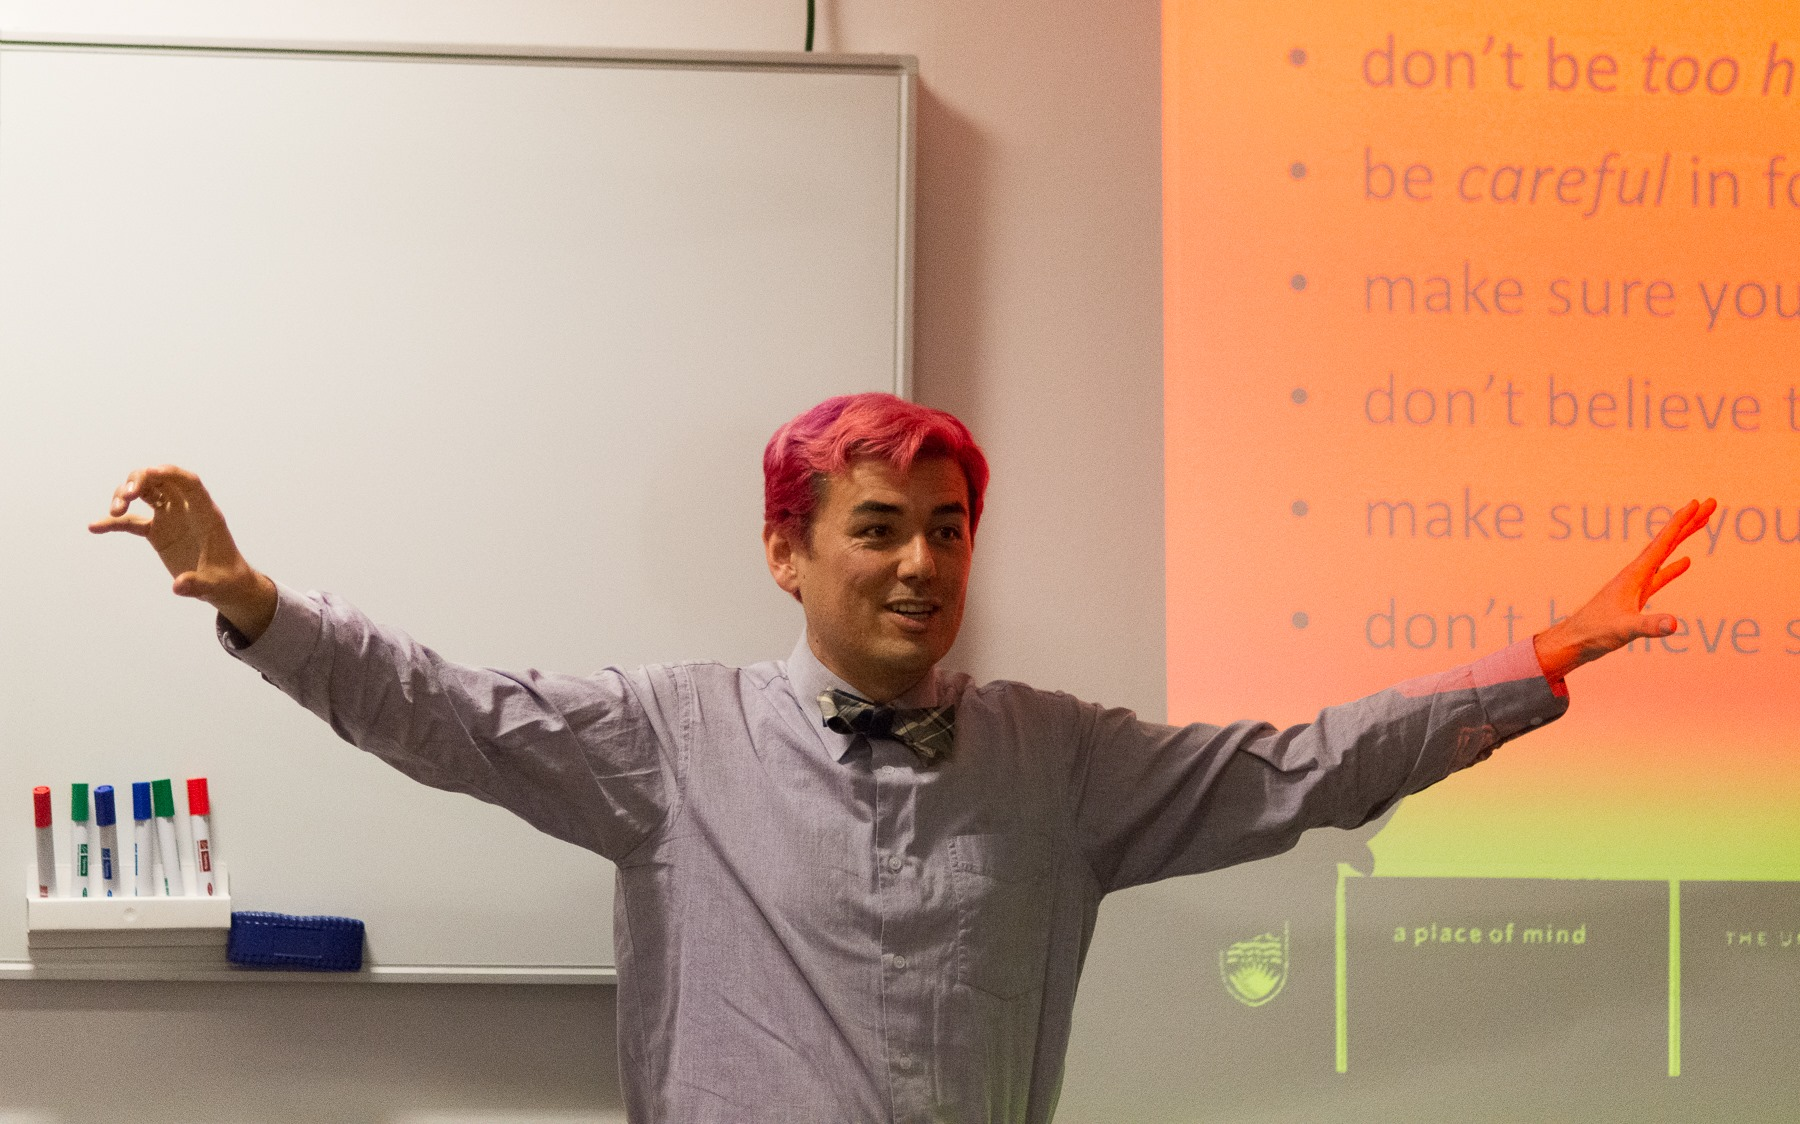
\includegraphics[width=\linewidth]{images/ichikawa.jpg}
  \centering
\end{figure}

{\sf
Jonathan Ichikawa, who modified the Magnus edition to create this version, would, first and foremost, like to thank P.D.\ Magnus. He is also grateful to Greg Restall, and his book \emph{Logic}, which is the first text he taught from and which is the model for the discussion of trees. He also thanks the many UBC students who test-drove drafts of the book. He's also grateful for helpful conversations with Roberta Ballarin, Roy Cook, Josh Dever, Dave Gilbert, Thony Gillies, and Jon Shaheen.

The original author, P.D.\ Magnus, would like to thank the people who made this project possible. Notable among these are Cristyn Magnus, who read many early drafts; Aaron Schiller, who was an early adopter and provided considerable, helpful feedback; {and} Bin Kang, Craig Erb, Nathan Carter, Wes McMichael, Selva Samuel, Dave Krueger, Brandon Lee, Toan Tran, and the students of Introduction to Logic, who detected various errors in previous versions of the book.
}

\vfill
{
\copyright\ \ifthenelse{\year=2005}{\number\year}{2005--\number\year} by P.D. Magnus and Jonathan Ichikawa. Some rights reserved.
}

{\footnotesize
You are free to copy this book, to distribute it, to display it, and to make derivative works, under the following conditions: (a) Attribution. You must give the original author credit. (b) Share Alike. If you alter, transform, or build upon this work, you may distribute the resulting work only under a license identical to this one. --- For any reuse or distribution, you must make clear to others the license terms of this work. Any of these conditions can be waived if you get permission from the copyright holder. Your fair use and other rights are in no way affected by the above. --- This is a human-readable summary of the full license, which is available on-line at \url{http://creativecommons.org/licenses/by-sa/3.0/}

Typesetting was carried out  in \LaTeX$2\varepsilon$. The style for natural deduction proofs is based on fitch.sty (v0.4) by Peter Selinger. Tree typesetting from prooftrees (v0.6) by Clea F. Rees. This copy of \forallx\ is current as of \today.
}
%!TEX root = forallx-ubc.tex
\chapter*{Preface to the UBC Edition}
\label{ch.preface}
\addcontentsline{toc}{chapter}{Preface to the UBC edition}


This preface outlines my approach to teaching logic, and explains the way this version of \emph{forall x} differs from Magnus's original. The preface is intended more for instructors than for students. 

I have been teaching logic at the University of British Columbia since 2011; starting in 2017, I decided to prepare this textbook, based on and incorporating much of P. D. Magnus's \emph{forall x}, which has been freely available for use and modification since 2005. Preparing this text had two main advantages for me: it allowed me to tailor the text precisely to my teaching preferences and emphasis, and, because it is available for free, it is saving money for students. (I encourage instructors to take this latter consideration pretty seriously. If you have a hundred students a year, requiring them each to buy a \$50 textbook takes \$5,000 out of students' pockets each year. If you teach with this or another free book instead, you'll save your students \$50,000 over ten years. It can be sort of annoying to switch textbooks if you're used to something already. But is staying the course worth \$50,000 of your students' money?)

This text was designed for a one-semester, thirteen-week course with no prerequisites. At UBC, the course has quite a mix of students with diverse academic backgrounds. For many it is their first philosophy course. As I teach Introduction to Formal Logic, the course has three central aims: (1) to help students think more clearly about arguments and argumentative structure, in a way applicable to informal arguments in philosophy and elsewhere; (2) to provide some familiarity and comfort with formal proof systems, including practice setting out formal proofs with each step justified by a syntactically-defined rule; and (3) to provide the conceptual groundwork for metatheoretical proofs, introducing the ideas of rigorous informal proofs about formal systems, preparing students for possible future courses focusing on metalogic and computability. I try to give those three elements roughly equal focus in my course, and in this book.

The book introduces two different kinds of formal proof systems --- analytic tableaux (`trees') and Fitch-style natural deduction. Unlike many logic texts, it puts its greater emphasis on trees. There are two reasons I have found this to be useful. One is that the algorithmic nature of tree proofs means that one can be assured to achieve successful proofs on the basis of patience and careful diligence, as opposed to requiring a difficult-to-quantify (and difficult-to-teach) `flash of insight'. The other is that the soundness and completeness theorems for tree methods are simpler and more intuitive than they are for natural deduction systems, and I find it valuable to expose students to proofs of significant metatheoretical results early in their logical studies. (I prove soundness and completeness for a sentential logic tree system in the fifth week of the semester.) As presented here, the soundness and completeness proofs emphasize contrasting the systems students learn with hypothetical alternative systems that modify the rules in various ways. A rule like this would undermine the soundness of the system, but not its completeness. If we changed the rules in this way, it would still be both sound and complete. Etc. This helps give intuitive substance to these theorems.

I also include a Fitch-style natural deduction system, both for sentential and quantified logic, both because its premise-conclusion form is particularly helpful for thinking about informal arguments, and because it is important to recognize and follow proofs laid out in that kind of format, for example in more advanced philosophical material. While students do learn to do Fitch-style proofs, I emphasize less of that puzzle-solving kind of skill here than in many textbooks.

The book begins with a systematic engagement with sentential logic in conventional ways: translations, sentential connectives, models, truth tables, and both proof systems, including soundness and completeness for the tree system. Students are thereby able to become familiar with all the central metalogical ideas, incorporating relatively simple logical symbolism, before introducing predicates, quantifiers, and identity. Once we enrich the language, we go through those previous ideas again, using our more complex vocabulary.

The first book I used for teaching was Greg Restall's \emph{Logic} (McGill--Queen's University Press, 2006), which I used for several years. My approach to teaching logic is heavily informed by that book; its influence in this text is particularly clear in the discussion of trees. (The natural deduction system I use is rather different from Restall's.)

In preparing this text, I began with Magnus's original and edited freely. There are sections where Magnus's prose has been retained entirely, and many of the exercises I have taken unchanged from the original. But I have also restructured many things and added quite a bit of new material. Unlike my version, which focuses on sentential logic before introducing predicates and quantification, Magnus's version integrated the discussion of sentential and quantificational systems, e.g.\ covering translation for both before discussing models and proofs for either. The original also did not include trees or soundness and completeness proofs. The two chapters on trees (\ref{ch.sl.trees} and \ref{ch.QLTrees}) and soundness and completeness (\ref{ch.SLsoundcomplete} and \ref{ch.QLsoundcomplete}) were written from scratch; my chapter on identity (\ref{ch.identity}) is also original. The other material in this edition incorporates Magnus's original material, some parts more heavily edited than others. I have slightly modified Magnus's natural deduction rules.

After a couple of years working with `beta' versions of the text online, I released the 1.0 version, along with the source code, in December 2018. The 2.0 version is new in summer 2020. The biggest changes in the latest round or revisions are in Chapter \ref{ch.ND.proofs}, where the order of presentation of the natural deduction rules has changed, and more examples have been added within the text. The rationale of the change was to start illustrating proofs earlier in the presentation of the rules. I've also put a bit more emphasis on the importance of exact matching of rule forms, and written a bit more precisely about the difference between SL proofs and proof schemas, when discussing derived rules. The other slightly substantive change I've made is to attend more precisely to how I'm using the term `interpretation' in the formal semantics for SL and QL. One of my aims is to emphasize the continuity between the two languages --- in my system, QL is literally a generalization of SL, and definitions of truth, entailment, etc., can be preserved. Various other smaller changes have been made as well, mostly stylistic changes and typo corrections.

Many thanks, first and foremost, to P.D.\ Magnus for providing this wonderful resource under a Creative Commons license, which made it freely available and gave me the right to modify and distribute it under the same licensing agreement. I hope other instructors will also feel free to either teach directly from this version, or to modify it to develop their own. The typesetting for trees is via Clea F.\ Rees's prooftrees package; thanks to her for making it available.

I'm grateful to the students in my 2017--20 PHIL 220 courses at UBC, who had an in-progress version of this book as their course textbook. They patiently and helpfully found and pointed out mistakes as I wrote them (incentivized, perhaps, by an offer of extra credit); this version has many fewer errors than it otherwise would have had. Thanks also to Cavell Chan and Joey Deeth, who did careful proofreading, and generated many solutions to exercises for the answer key, and to Laura Greenstreet for LaTeX and other technical help. These three assistants were supported by a UBC Library Open Access Grant in 2018--19.

I am maintaining a list of known issues and errors for this book, to be corrected in future editions, under `issues' at \url{https://github.com/jonathanichikawa/for-all-x}. If you see any mistakes, please feel free to add them there directly, or to email me with them. The most recent version of the book is also always available for download there too.

\begin{flushright}
Jonathan Ichikawa \\
University of British Columbia \\
July 2020 \\
ichikawa@gmail.com
\end{flushright}

{
\setlength{\parskip}{0em}
\setlength{\cftsecnumwidth}{3em}
\tableofcontents
}

%!TEX root = forallx-ubc.tex
\chapter{What is logic?}
\label{ch.intro}

Logic is the business of evaluating arguments, sorting good ones from bad ones. In everyday language, we sometimes use the word `argument' to refer to belligerent shouting matches. If you and a friend have an argument in this sense, things are not going well between the two of you. This is not the kind of `argument' that will concern us. Arguments in the logical sense aren't events that happen between people; a logical argument is structured to give someone a reason to believe some conclusion. Here are two examples of such arguments:

\label{argRaining}
\begin{earg}
\item[(1)] It is raining heavily.
\item[(2)] When it rains, everyone outside without an umbrella gets wet.
\item[\therefore] You should take an umbrella.
\end{earg}


\label{argSnowing}
\begin{earg}
\item[(1)] It is either raining or snowing.
\item[(2)] If it is colder than -10 degrees, it is not raining.
\item[(3)] It is -18 degrees.
\item[\therefore] It is snowing.
\end{earg}
 
The three dots on the last line of each argument mean `Therefore' and they indicate that the final sentence is the \textsl{conclusion} of the argument. The other sentences are \textsl{premises} of the argument. If you believe the premises, then the argument provides you with a reason to believe the conclusion.

This chapter discusses some basic logical notions that apply to arguments in a natural language like English. It is important to begin with a clear understanding of what arguments are and of what it means for an argument to be valid. Later we will translate arguments from English into a formal language. We want formal validity, as defined in the formal language, to have at least some of the important features of natural-language validity.

\section{Arguments}
A crucial part of analyzing an argument is identifying its conclusion. Every argument has a conclusion --- the conclusion is the claim the argument is trying to establish. Premises are starting-points, used to lend support to the conclusion. Often, the conclusion will be signified by words like `so' or `therefore'. Premises might be marked by words like `because'. These words can give a clue as to just what the argument is supposed to be.

\begin{description}
\item[premise indicators:] since, because, given that
\item[conclusion indicators:] therefore, hence, thus, then, so
\end{description}
\nix{could expand this list}

In a natural language like English, \emph{sometimes}, arguments start with their premises and end with their conclusions, but not always. For some purposes in this course, we will be working with \emph{idealizations} of natural language, where we work as if some generally applicable rules of thumb held without exception. Let's define (a slightly technical notion of) an \define{argument} as a series of sentences. The sentences at the beginning of the series are premises. The final sentence in the series is the conclusion.

Here is an example of an argument:

\begin{earg}
\item[] People get wet whenever it rains.
\item[] It often rains in Vancouver.
\item[\therefore] People often get wet in Vancouver.
\end{earg}

The idea of an argument is that the premises are supposed to give you reason to accept the conclusion. If I'm trying to convince you that people often get wet in Vancouver --- the conclusion of the argument above --- convincing you of the two premises might be a good way to get you there.

Notice that our definition of an argument is quite general. Consider this example:
\begin{earg}
\item[] Vancouver has more churches than any other Canadian city.
\item[] Two oboes are fighting a duel under the fireworks.
\item[\therefore] J.\ Edgar Hoover was an honest man.
\end{earg}

It may seem odd to call this an argument, but that is because it would be a {terrible} argument. The two premises have nothing at all to do with the conclusion. (Moreover, they aren't very plausible.) Nevertheless, given our definition, it still counts as an argument --- albeit a bad one. One of our central aims in formal logic is to provide rigorous, formal tests for evaluating arguments.


\section{Sentences and propositions}
\label{intro.sentences}

The premises and conclusions of arguments are sentences. But not just any English sentence is suitable for figuring into an argument. For example, questions count as grammatical sentences of English, but logical arguments never have questions as premises or conclusions. We are interested especially in sentences that can be true or false. Think of these as the sentences that purport to describe the way things are. Such sentences are sometimes described as expressing \emph{propositions}.

We will not be theorizing in terms of questions and other non-propositional sentences in formal logic. Since we are only interested in sentences that can figure as a premise or conclusion of an argument, we'll define a technical notion of a \define{sentence} as a sentence expressing a proposition, i.e., a sentence that can be true or false.

Don't confuse the idea of a sentence that can be true or false with the difference between fact and opinion. Often, sentences in logic will express things that would count as facts --- such as `Kierkegaard was a hunchback' or `Kierkegaard liked almonds.' They can also express things that you might think of as matters of opinion --- such as, `Almonds are yummy' or `the U.S.\ invasion of Iraq was unjustified'. These are all examples of things that are either true or false.

It is also important to keep clear the distinction between something's being \emph{true} and something's being \emph{known}. A sentence is the kind of thing that can be true or false; that doesn't mean you'll always be able to tell whether it is true or false. For example, `there are an even number of humans on Earth right now' is a sentence. It is either true or false, even though it is pretty much impossible to tell which. Similarly, there are controversial propositions, where people disagree about whether they are true or false, and where it seems very difficult to settle the debate. (I think that `Freedom of expression requires restricting oppressive speech' is an example.) This is either true or false, even if debates about which it is aren't likely to resolve the question. So it counts as a propositional sentence.

What are some examples of grammatical English sentences that do not express propositions? We've discussed one category already:

\paragraph{Questions} In a grammar class, `Are you sleepy yet?' would count as an interrogative sentence. Although you might be sleepy or you might be alert, the question itself is neither true nor false. So `Are you sleepy yet?' is not a sentence in our technical, propositional sense. Suppose you answer the question: `I am not sleepy.' This \emph{is} either true or false, and so it \emph{is} a sentence in the logical sense. Generally, \emph{questions} will not count as sentences, but \emph{answers} will. 

`What is this course about?' is not a sentence. `No one knows what this course is about' is a sentence.

\paragraph{Imperatives} Commands are often phrased as imperatives like `Wake up!', `Sit up straight', and so on. In a grammar class, these would count as imperative sentences. Although it might be good for you to sit up straight or it might not, the command is neither true nor false. Note, however, that commands are not always phrased as imperatives. `You will respect my authority' \emph{is} either true or false --- either you will or you will not --- and so it counts as a sentence in the logical sense.

\paragraph{Exclamations} Expressions like `Ouch!' or `Boo, Yankees!' are sometimes described as exclamatory sentences, but they are neither true nor false. We will treat `Ouch, I hurt my toe!' as meaning the same thing as `I hurt my toe.' The `ouch' does not add anything that could be true or false.

To recap: \emph{sentences}, in the technical sense we're interested in, are claims that can be true or false. One pretty good test you can run to see whether something is a sentence is to ask whether it makes sense to insert `it is true that' or `it is false that' in front of it. It's perfectly fine to say `it is true that Kierkegaard liked almonds' or `it is true that the U.S.\ invasion of Iraq was unjustified'. But it doesn't make sense to say `it is true that are you sleepy yet' or `it is true that sit up straight'.

We will call truth or falsity the \define{truth-value} of a sentence.



\section{Two ways that arguments can go wrong}
Consider the argument that you should take an umbrella (on p.~\pageref{argRaining}, above).

\begin{earg}
\item[(1)] It is raining heavily.
\item[(2)] When it rains, everyone outside without an umbrella gets wet.
\item[\therefore] You should take an umbrella.
\end{earg}

If premise (1) is false --- if it is sunny outside --- then the argument fails. It does not establish that you should take an umbrella. Or suppose that premise (2) is false. Maybe not everyone without an umbrella gets wet. (Maybe some people are able to stay under the awnings.) In this case, too, the argument does not establish its conclusion. Arguments only succeed when all their premises are true.

Suppose both premises \emph{are} true. It really is raining heavily, and we're talking about an area where there's no protection from the rain other than umbrellas, so that anyone outside without an umbrella will get wet when it rains. Now does the argument show you that you should take an umbrella? It certainly seems to lend some support in that direction. But notice that it's still not \emph{conclusive}. There are still \emph{possible} ways the conclusion might be false. For example, suppose you like getting wet. Then, even if it is raining heavily, and even if everyone who goes outside without an umbrella when it rains gets wet, maybe you have no reason to take the umbrella.

A good argument --- or at least, an argument that is good in one particularly interesting way --- \emph{compels} its conclusion.

So it seems that there are two ways an argument could be weak. First, one or more of the premises might be false. An argument gives you a reason to believe its conclusion only if you believe its premises. Second, the premises might fail to support the conclusion, or fail to support it sufficiently strongly. Even if the premises were true, the form of the argument might be weak. The example we just considered is weak in both ways.

Once again, we are working with a particular kind of idealization regarding arguments and what makes them good. Consider another example:
\begin{earg}
\item[] You are reading this book.
\item[] This is a logic book.
\item[\therefore] You are a logic student.
\end{earg}
In a straightforward and ordinary sense, this is not a terrible argument. The premises are true. And they do offer some support for the conclusion. Most people who read this book are logic students. Still, it is \emph{possible} for someone besides a logic student to read this book. If the deans carefully read this book in order to find out whether I'm criticizing the UBC administration, that wouldn't make them logic students. So the premises of this argument, even though they are true, do not guarantee the truth of the conclusion.

By contrast, the sample argument about snow \emph{is} valid. There's just no possible way for all three of its premises to be true without it snowing.

In logic, we are interested in arguments whose premises \emph{guarantee} their conclusions. We call such arguments `deductively valid' or just `valid.' Even though we might count the rain argument, or the logic book argument, as a good argument in some sense, they are not valid; that is, they are `invalid.' One important task of logic is to sort valid arguments from invalid arguments.

\section{Validity}
\label{sec:validity}
An argument is deductively \define{valid} if and only if it is impossible for all the premises to be true while the conclusion is false. (We'll say a bit more about just what we mean by `impossible' in \S\ref{sec.impossible} below.)

That's our official \emph{definition} of validity. Once again (get used to this pattern), our formal definition is related to, but not quite the same as, the ordinary colloquial notion with the same name. In ordinary English, to say something is `valid' means, somewhat vaguely, that it is good. (Think of a `valid point' or a `valid perspective'.) In logic, a valid argument is one that has this very specific feature: it's impossible for the premises to be true if the conclusion is false. (Side note: this is a good terminological distinction to keep in mind when writing essays in philosophy courses. Philosophy professors tend to wince and get annoyed when students use the word `valid' in its imprecise sense. You can help stay on their good sides by only saying something is `valid' when you mean that it is an argument whose premises are inconsistent with the falsity of its conclusion.)

Notice that validity does \emph{not} require that the premises be true. Consider this example:

\begin{earg}
\item[(1)] Oranges are either fruits or musical instruments.
\item[(2)] Oranges are not fruits.
\item[\therefore] Oranges are musical instruments.
\end{earg}

This is a valid argument. It is impossible for the premises to be true if the conclusion is false. Since it has a false premise --- premise (2) --- it does not actually establish its conclusion, but it does have a \emph{valid logical form}. \emph{If} both premises were true, \emph{then} the conclusion would necessarily be true.

Since this is a valid argument that is, in some important sense, a bad argument, this shows that validity isn't the only feature we care about in arguments. An argument is \define{sound} if and only if it is valid and all of its premises are true. For example, this variant argument on the above argument is sound:

\begin{earg}
\item[(1)] Oranges are either fruits or musical instruments.
\item[(2)] Oranges are not musical instruments.
\item[\therefore] Oranges are fruits.
\end{earg}

 For reasons that will emerge, logic tends to focus primarily on validity, rather than soundness.

We've seen that a valid argument does not need to have true premises or a true conclusion. Conversely, having true premises and a true conclusion is also not enough to make an argument valid. Consider this example:

\begin{earg}
\item[] Donald Trump is a U.S.\ citizen.
\item[] Justin Trudeau is a Canadian citizen.
\item[\therefore] UBC is the largest employer in Vancouver.
\end{earg}

The premises and conclusion of this argument are, as a matter of fact, all true. Nevertheless, this is quite a poor argument. This is related to the fact that the premises have nothing to do with the conclusion. More precisely, the definition of validity is not satisfied: it is possible for the premises to be true while the conclusion is false. Although the conclusion is \emph{actually} true, it is \emph{possible} for the premises of this argument to be true while the conclusion is false. We may imagine, for example, that Lululemon hired an additional 100,000 employees in Vancouver, while UBC remained the same size, and without any world leaders changing their citizenship statuses. In such a possible scenario, the premises would be true, while the conclusion is false.

The important thing to remember is that validity is not about the actual truth or falsity of the sentences in the argument. Instead, it is about the form of the argument: The truth of the premises is incompatible with the falsity of the conclusion.

Here are some more valid arguments. Can you see why each is valid?

\begin{earg}
\item Socrates is a man.
\item All men are carrots.
\item[\therefore] Socrates is a carrot.
\end{earg}


\begin{earg}
\item Abe Lincoln was either born in Illinois or he was once president.
\item Abe Lincoln was never president.
\item[\therefore] Abe Lincoln was born in Illinois.
\end{earg}

\begin{earg}
\item Justin Trudeau is either from France or from Luxembourg.
\item Justin Trudeau is not from Luxembourg.
\item[\therefore] Justin Trudeau is from France.
\end{earg}


\begin{earg}
\item If the world were to end today, then I would not need to get up tomorrow morning.
\item I will need to get up tomorrow morning.
\item[\therefore] The world will not end today.
\end{earg}


%\subsection{Inductive arguments}
%
%There can be good arguments which nevertheless fail to be deductively valid. Consider this one:
%
%\begin{earg}
%\item[] In January 1997, it rained in San Diego.
%\item[] In January 1998, it rained in San Diego.
%\item[] In January 1999, it rained in San Diego.
%\item[\therefore] It rains every January in San Diego.
%\end{earg}
%
%This is an \define{inductive} argument, because it generalizes from many cases to a conclusion about all cases.
%
%Certainly, the argument could be made stronger by adding additional premises: In January 2000, it rained in San Diego. In January 2001$\ldots$ and so on. Regardless of how many premises we add, however, the argument will still not be deductively valid. It is possible, although unlikely, that it will fail to rain next January in San Diego. Moreover, we know that the weather can be fickle. No amount of evidence should convince us that it rains there \emph{every} January. Who is to say that some year will not be a freakish year in which there is no rain in January in San Diego; even a single counter-example is enough to make the conclusion of the argument false.
%
%Inductive arguments, even good inductive arguments, are not deductively valid. We will not be interested in inductive arguments in this book.

\section{Impossibility}
\label{sec.impossible}

The definition of validity centrally invokes the notion of impossibility. What it means for a sentence to be \emph{impossible} is that there is no possible way for it to be true. Impossible sentences don't just \emph{happen} to be false; they \emph{must} be false. Consider the sentence, `The Whitecaps lost their last game.' As it happens, at the time I'm writing, that's false. They actually won. But it's not impossible; they might have lost, if a few things had gone differently. So that sentence is false, but not impossible.

By contrast, blatant contradictions like `the Whitecaps won the game and the Whitecaps lost the game' \emph{are} impossible. This sentence doesn't just \emph{happen} to be false. It couldn't \emph{possibly} be true.

Even falsehoods that are really obviously false, and for which it's hard to imagine how they could be true, might be \emph{possible}. It's not \emph{impossible} that pigs could fly. Someone might invent powerful wings for them. When we're interested in impossible sentences in logic, we really mean \emph{impossible}. The best examples are contradictions.

So to apply the definition of validity, we consider whether there is any possibility, no matter how far-fetched, where the premises are true and the conclusion is false.

\section{Other logical notions}

Here are a few more relevant terms we'll be working with.

\subsection{Logical truth}
\label{sec-tautologydef}
In considering arguments formally, we care about what would be true \emph{if} the premises were true. Generally, we are not concerned with the actual truth value of any particular sentences --- whether they are \emph{actually} true or false. (As indicated above, we will be more interested in validity than in soundness.) Yet there are some sentences that must be true, just as a matter of logic.

Compare these sentences:
\begin{earg}
\item[\ex{Acontingent}] It is raining.
\item[\ex{Atautology}] Either it is hot outside, or it is not hot outside.
\item[\ex{Acontradiction}] There is an earthquake happening here right now and there are never earthquakes here.
\end{earg}
Sentence \ref{Acontingent} could be true or it could be false. (As I'm typing these words on a sunny Vancouver summer day, it is false.) Sentences that could be true, or could be false, are called \emph{contingent} sentences.

Sentence \ref{Atautology} is different. Even though I don't know what the weather is like as you're reading this book, I still know that it's true. Sentence \ref{Atautology} \emph{must} be true. This sentence is \emph{logically true}; no matter how the weather or anything else happens to be, this sentence has to be true. We call a sentence like this a \define{logical truth} or a \define{tautology}.

You do not need to check the weather to know about sentence \ref{Acontradiction}, either. It must be false, simply as a matter of logic. There could be an earthquake now, but if so, it couldn't be the case that there are never earthquakes here. Or there might never be any earthquakes, but if so, there couldn't be one now. The third sentence is \define{logically false}; it is false regardless of what the world is like. A logically false sentence is called a \define{contradiction}.

I said above that a contingent sentence could be true and it also could be false. We can also define contingency in terms of tautologies and contradictions thus: a \define{contingent sentence} is a sentence that is neither a tautology nor a contradiction.

%A sentence might \emph{always} be true and still be contingent. For instance, if there never were a time when the universe contained fewer than seven things, then the sentence `At least seven things exist' would always be true. Yet the sentence is contingent; its truth is not a matter of logic. There is no contradiction in considering a possible world in which there are fewer than seven things. The important question is whether the sentence \emph{must} be true, just on account of logic.

\subsection{Logical equivalence}
We can also ask about the logical relations \emph{between} two sentences. For example:
\begin{earg}
\item[] Sunil went to the store after he washed the dishes.
\item[] Sunil washed the dishes before he went to the store.
\end{earg}
These two sentences are both contingent. (Do you see why?) Yet they must have the same truth-value. If either of the sentences is true, then they both are; if either of the sentences is false, then they both are. When two sentences necessarily have the same truth value, we say that they are \define{logically equivalent}.

Notice that both of these arguments are valid:

\begin{earg}
\item[] Sunil went to the store after he washed the dishes.
\item[\therefore] Sunil washed the dishes before he went to the store.
\end{earg}


\begin{earg}
\item[] Sunil washed the dishes before he went to the store.
\item[\therefore] Sunil went to the store after he washed the dishes.
\end{earg}

In general, if two sentences are equivalent, then an argument with either one as a premise, and the other as the conclusion, will be valid.

\subsection{Consistency}
Consider these two sentences:
\begin{ekey}
\item[B1] My only brother is taller than I am.
\item[B2] My only brother is shorter than I am.
\end{ekey}
Logic alone cannot tell us which, if either, of these sentences is true. Yet we can say that \emph{if} the first sentence (B1) is true, \emph{then} the second sentence (B2) must be false. And if B2 is true, then B1 must be false. It cannot be the case that both of these sentences are true.

If a set of sentences could not all be true at the same time, like B1--B2, they are said to be \define{inconsistent}. Otherwise, they are \define{consistent}.

We can ask about the consistency of any number of sentences. For example, consider the following list of sentences:
\label{MartianGiraffes}
\begin{ekey}
\item[G1] There are at least four giraffes at the wild animal park.
\item[G2] There are exactly seven gorillas at the wild animal park.
\item[G3] There are not more than two Martians at the wild animal park.
\item[G4] Every giraffe at the wild animal park is a Martian.
\end{ekey}
G1 and G4 together imply that there are at least four Martian giraffes at the park. This conflicts with G3, which implies that there are no more than two Martian giraffes there. So the set of sentences G1--G4 is inconsistent. (Notice that in this example the inconsistency has nothing at all to do with G2. G2 just happens to be part of an inconsistent set.)


\section{Formal languages}

%Here is a famous valid argument:
%\begin{earg}
%\item[] Socrates is a man.
%\item[] All men are mortal.
%\item[\therefore] Socrates is mortal.
%\end{earg}
%This is an iron-clad argument. The only way you could challenge the conclusion is by denying one of the premises --- the logical form is impeccable. What about this next argument?
%
%\begin{earg}
%\item[] Socrates is a man.
%\item[] All men are carrots.
%\item[\therefore] Socrates is a carrot.
%\end{earg}
%
%This argument might be less interesting than the first, because the second premise is obviously false. There is no clear sense in which all men are carrots. Yet the argument is valid. To see this, notice that both arguments have this form:
%
%\begin{earg}
%\item[] $S$ is $M$.
%\item[] All $M$s are $C$s.
%\item[\therefore] $S$ is $C$.
%\end{earg}
%
%In both arguments $S$ stands for Socrates and $M$ stands for man. In the first argument, $C$ stands for mortal; in the second, $C$ stands for carrot. Both arguments have this form, and every argument of this form is valid. So both arguments are valid.

%\subsection{Aristotelean logic}
%
%What we did here was replace words like `man' or `carrot' with symbols like `M' or `C' so as to make the logical form explicit. This is the central idea behind formal logic. We want to remove irrelevant or distracting features of the argument to make the logical form more perspicuous.
%
%Starting with an argument in a \emph{natural language} like English, we translate the argument into a \emph{formal language}. Parts of the English sentences are replaced with letters and symbols. The goal is to reveal the formal structure of the argument, as we did with these two.
%
%There are formal languages that work like the symbolization we gave for these two arguments. A logic like this was developed by Aristotle, a philosopher who lived in Greece during the 4th century BC. Aristotle was a student of Plato and the tutor of Alexander the Great. Aristotle's logic, with some revisions, was the dominant logic in the western world for more than two millennia.
%
%In Aristotelean logic, categories are replaced with capital letters. Every sentence of an argument is then represented as having one of four forms, which medieval logicians labeled in this way: (A) All $A$s are $B$s. (E) No $A$s are $B$s. (I) Some $A$ is $B$. (O) Some $A$ is not $B$.
%
%It is then possible to describe valid \emph{syllogisms}, three-line arguments like the two we considered above. Medieval logicians gave mnemonic names to all of the valid argument forms. The form of our two arguments, for instance, was called \emph{Barbara}. The vowels in the name, all As, represent the fact that the two premises and the conclusion are all (A) form sentences.
%
%There are many limitations to Aristotelean logic. One is that it makes no distinction between kinds and individuals. So the first premise might just as well be written `All $S$s are $M$s': All Socrateses are men. Despite its historical importance, Aristotelean logic has been superceded. The remainder of this book will develop two formal languages.

So far, we have been working with arguments expressed in English. But there are some general argumentative structures that transcend English or any other particular natural language. Consider, for example, the following simple argument:

\begin{earg}
\item[] Vancouver is in Canada.
\item[] Moscow is in Russia.
\item[\therefore] Vancouver is in Canada and Moscow is in Russia.
\end{earg}

Hopefully by now it is obvious to you that this argument is valid. (Not just that --- it is even sound.) That argument has something important in common with this one:

\begin{earg}
\item[] Vancouver is on Mars.
\item[] Moscow is on Venus.
\item[\therefore] Vancouver is on Mars and Moscow is on Venus.
\end{earg}

Although this one has false premises, and so can't be sound, it is also valid. It is impossible for the premises to be true if the conclusion is false. Not only that --- it seems that the argument is valid in, in a sense to be articulated, \emph{exactly the same way}. The validity of the first argument is very similar to that of the second. Even though they are expressed by different strings of English sentences, it is useful to develop a language that emphasizes the interesting respects in which they are the same. Over the course of this textbook, we'll be developing and working with such a language. We'll begin with a simple version of our logical language, called SL, for \emph{sentential logic}. Later on, we'll develop a more complicated logical language, QL, for \emph{quantified logic}. Both languages are \emph{formal} in the sense that there are precise rules that govern how we should evaluate sentences within them.

%\subsection{Why there are different formal languages}
%When we translate an argument into a formal language, we hope to make its logical structure clearer. We want to include enough of the structure of the English language argument so that we can judge whether the argument is valid or invalid. If we included every feature of the English language, all of the subtlety and nuance, then there would be no advantage in translating to a formal language. We might as well think about the argument in English.
%
%At the same time, we would like a formal language that allows us to represent many kinds of English language arguments. This is one reason to prefer QL to Aristotelean logic; QL can represent every valid argument of Aristotelean logic and more.

English is a natural language, not a formal one. Its rules are vague and messy, and constantly changing. We will spend some time translating between English and our formal languages, but the translations will not always be precise. There is a tension between wanting to capture as much of the structure of English as possible and wanting a simple formal language with tractable rules --- simpler formal languages will approximate natural languages less closely. There is no perfect formal language. Some will do a better job than others in translating particular English-language arguments.

In this book, we make the assumption that \emph{true} and \emph{false} are the only possible truth-values. Logical languages that make this assumption are called \emph{bivalent}, which means \emph{two-valued}. SL and QL are both bivalent, but some philosophers have emphasized limits to the power of bivalent logic. Some logics, beyond the scope of this book, allow for sentences that are neither true nor false. Others allow for sentences that are both true \emph{and} false. Our logical system, which is often called \emph{classical logic}, will give every sentence exactly one truth value: either true or false.


\section*{Summary of logical notions}
\begin{itemize}

\item An \define{argument} is a structured set of sentences, with \emph{premises} intended to offer support for a \emph{conclusion}.

\item A \define{sentence}, in our logical terminology, is a sentence that expresses a proposition, and can be either true or false.

\item An argument is (deductively) \define{valid} if it is impossible for the premises to be true and the conclusion false; it is \define{invalid} otherwise.

\item A \define{tautology} is a sentence that must be true, as a matter of logic.

\item A \define{contradiction} is a sentence that must be false, as a matter of logic.

\item A \define{contingent sentence} is neither a tautology nor a contradiction.

\item Two sentences are \define{logically equivalent} if they necessarily have the same truth value.

\item A set of sentences is \define{consistent} if it is logically possible for all the members of the set to be true at the same time; it is \define{inconsistent} otherwise.
\end{itemize}


\practiceproblems
At the end of each chapter, you will find a series of practice problems that review and explore the material covered in the chapter. There is no substitute for actually working through some problems, because logic is more about a way of thinking than it is about memorizing facts. The answers to some of the problems are provided at the end of the book in appendix \ref{app.solutions}; the problems that are solved in the appendix are marked with a \solutions.

\solutions
\problempart
\label{pr.Sentences1}
Which of the following are `sentences' in the logical sense?
\begin{earg}
\item England is smaller than China.
\item Greenland is south of Jerusalem.
\item Is New Jersey east of Wisconsin?
\item The atomic number of helium is 2.
\item The atomic number of helium is $\pi$.
\item I hate overcooked noodles.
\item Blech! Overcooked noodles!
\item Overcooked noodles are disgusting.
\item Take your time.
\item This is the last question.
\end{earg}

\problempart
\label{hw1.B}
Which of the following are `sentences' in the logical sense?
	\begin{earg}
		\item I would like a double cheeseburger with no onions.
		\item Thank you very much for that gracious reception.
		\item If you strike me down, I shall become more powerful than you could possibly imagine.
		\item There are more trees at UBC than there are flowers in my office and my Uncle Jack really seems to like drinking apple juice, or if that's not apple juice, then he really seems to like whatever it is that he's drinking, but anyway, what I'm really trying to say is, I'm hungry and I could really go for a burger or a bag of scorpions right about now.
		\item I did it.
		\item No invalid arguments have impossible premises.
	\end{earg}

\problempart
\label{pr.EnglishTautology}
For each of the following: Is it a tautology, a contradiction, or a contingent sentence?
\begin{earg}
\item Caesar crossed the Rubicon.
\item Someone once crossed the Rubicon.
\item No one has ever crossed the Rubicon.
\item If Caesar crossed the Rubicon, then someone has.
\item Even though Caesar crossed the Rubicon, no one has ever crossed the Rubicon.
\item If anyone has ever crossed the Rubicon, it was Caesar.
\end{earg}

\solutions
\problempart
\label{pr.MartianGiraffes}
Look back at the sentences G1--G4 on p.~\pageref{MartianGiraffes}, and consider each of the following sets of sentences. Which are consistent? Which are inconsistent?
\begin{earg}
\item G2, G3, and G4
\item G1, G3, and G4
\item G1, G2, and G4
\item G1, G2, and G3
\end{earg}

\solutions
\problempart
\label{pr.EnglishCombinations}
Which of the following is possible? If it is possible, give an example. If it is not possible, explain why.
\begin{earg}
\item A valid argument that has one false premise and one true premise
\item A valid argument that has a false conclusion
\item A valid argument, the conclusion of which is a contradiction
\item An invalid argument, the conclusion of which is a tautology
\item A tautology that is contingent
\item Two logically equivalent sentences, both of which are tautologies
\item Two logically equivalent sentences, one of which is a tautology and one of which is contingent
\item Two logically equivalent sentences that together are an inconsistent set
\item A consistent set of sentences that contains a contradiction
\item An inconsistent set of sentences that contains a tautology
\end{earg}


\problempart
\label{hw1.C}
For each, give an argument with the indicated features, or explain why it is impossible to do so:
	\begin{earg}
		\item Valid, but not sound.
		\item Valid, with an impossible conclusion.
		\item Sound, with an impossible premise.
		\item Sound, and an instance of this form:
			\begin{earg}
				\item[] if $P$ then Q
				\item[] R
				\item[\therefore] $Q$
			\end{earg}
	\end{earg}


\problempart
\label{pr.ImpossiblePremises}
Is this argument valid? Why or why not? (Hint: here and elsewhere in logic, read the definitions of our formal terms literally.)
\begin{earg}
\item[(1)] PHIL 220 is a course with a final exam.
\item[(2)] No courses ever have final exams.
\item[\therefore] Everyone is going to get an A+ in PHIL 220.
\end{earg}

\problempart
\label{hw1.A}
For each, indicate whether it is true or false.
	\begin{earg}
		\item All arguments with true premises and true conclusions are sound.
		\item Only valid arguments are sound.
		\item If an argument to the conclusion $A$ is sound, then an argument to the conclusion not $A$ is not sound.
		\item All arguments with at least one impossible premise are valid.
		\item All invalid arguments are instances of invalid argument forms.
		\item No invalid arguments have impossible premises.
	\end{earg}

%!TEX root = forallx-ubc.tex
\chapter{Sentential logic}
\label{ch.SL}




This chapter introduces a logical language called SL. It is a version of \emph{sentential logic}, because the basic units of the language will represent entire sentences. (Recall from \S\ref{intro.sentences} that we're only considering propositional sentences.)



\section{Sentence letters}
In SL, capital Roman letters ($A$, $B$, $C$, etc.) are used to represent basic sentences. Considered only as a symbol of SL, the letter $A$ could mean any sentence. So when translating from English into SL, it is important to provide a \emph{symbolization key}. The key provides an English language sentence for each sentence letter used in the symbolization.

For example, consider this argument:
\begin{earg}
\item[] Today is New Year's Day.
\item[] If today is New Year's Day, then people are swimming in English Bay.
\item[\therefore] People are swimming in English Bay.
\end{earg}

This is obviously a valid argument in English. In symbolizing it, we want to preserve the structure of the argument that makes it valid.
What happens if we replace each sentence with a letter? Our symbolization key would look like this:

\begin{ekey}
\item[A:]Today is New Year's Day.
\item[B:]If today is New Year's Day, then people are swimming in English Bay.
\item[C:]People are swimming in English Bay.
\end{ekey}

We could then symbolize the argument in this way:
\begin{earg}
\item[] $A$
\item[] $B$
\item[\therefore] $C$
\end{earg}
This is a possible way to symbolize this argument, but it's not a very interesting one. There is no necessary connection between some sentence $A$, which could be any sentence, and some other sentences $B$ and $C$, which could be any sentences. Something important about the argument has been lost in translation. The original argument was valid, but this translation of the argument does not reflect that validity. Given a different symbolization key, for example, the same argument form 

\begin{earg}
\item[] $A$
\item[] $B$
\item[\therefore] $C$
\end{earg}

could equally well stand in for this invalid argument:

\begin{ekey}
\item[]Today is Christmas Day.
\item[]Tiny Tim has difficulty walking without crutches.
\item[\therefore]We're all going to die tomorrow.
\end{ekey}

A more interesting translation of the valid New Year's argument will show how it is different from the invalid Christmas argument. The relevant thing about the New Year's argument is that the second premise is not just \emph{any} sentence. Notice that the second premise contains the first premise and the conclusion \emph{as parts}. Our symbolization key for the argument only needs to include meanings for $A$ and $C$, and we can build the second premise from those pieces. So we symbolize the argument this way:
\begin{earg}
\item[] $A$
\item[] If $A$, then $C$.
\item[\therefore] $C$
\end{earg}
This preserves the structure of the argument that makes it valid, but it still makes use of the English expression `If$\ldots$ then$\ldots$'. For our formal language, we ultimately want to replace all of the English expressions with logical notation, but this is a good start.

The sentences that can be symbolized with sentence letters are called \emph{atomic sentences}, because they are the basic building blocks out of which more complex sentences can be built. Whatever logical structure a sentence might have is lost when it is translated as an atomic sentence. From the point of view of SL, the sentence is just a letter. It can be used to build more complex sentences, but it cannot be taken apart.

%Atomic sentences go together to make complex sentences in much the same way that physical atoms go together to make molecules. Physical atoms were originally called `atoms' because chemists thought that they were irreducible. Chemists were wrong, and physical atoms can be split.

%It is important to remember that a symbolization key only gives the meaning of atomic sentences for purposes of translating a specific argument.

We use capital Roman alphabet letters to represent SL sentences. There are only twenty-six such letters. We don't want to impose this artificial limit onto our formal language; it's better to work with a language that allows an arbitrary number of atomic sentences. To achieve this, we allow atomic sentences that have a capital letter with a numeric subscript. So we could have a symbolization key that looks like this:

\begin{ekey}
\item[A$_1$:] Aang is from the Air Nation.
\item[A$_2$:] Aang is vegetarian.
\item[A$_3$:] Aang can bend water.
\item[T$_1$:] Toph is blind.
\item[T$_2$:] Toph likes badgers.
\item[T$_3$:] Toph invented metal bending.
\end{ekey}

Keep in mind that each of these is a different atomic sentence. Although it is often convenient, for making it easier to remember what each letter stands for, to use letters corresponding to the sentences' subject matters, as in the example above, no such requirement is built into the rules of SL. There is no special relationship between $A_{1}$ and $A_{2}$, as far as SL goes. It's just for our convenience that we might choose to make all the $A$ sentences about Aang.

\section{Connectives}
Logical connectives are used to build complex sentences from atomic components. There are five logical connectives in SL. This table summarizes them. They are explained below.

\begin{table}[h]
\center
\begin{tabular}{|c|c|c|}
\hline
symbol&what it is called&rough translation\\
\hline
\enot&negation&`It is not the case that$\ldots$'\\
\eand&conjunction&`Both$\ldots$\ and $\ldots$'\\
\eor&disjunction&`Either$\ldots$\ or $\ldots$'\\
\eif&conditional&`If $\ldots$\ then $\ldots$'\\
\eiff&biconditional&`$\ldots$ if and only if $\ldots$'\\
\hline
\end{tabular}
\end{table}

Natural languages like English are vague and imprecise, and carry many complex subtleties of meaning. Our formal language, SL, has none of these properties. It is defined by precise rigid rules. Consequently, the `translation' provided in the table is only an approximate one. We'll see some of the differences below.

\section{Negation}
Consider how we might symbolize these sentences:
\begin{earg}
\item[\ex{not1}] Logic is hard.
\item[\ex{not2}] It is false that logic is hard.
\item[\ex{not3}] Logic isn't hard.
\end{earg}

In order to symbolize sentence \ref{not1}, we will need one sentence letter. We can provide a symbolization key:

\begin{ekey}
\item[H:]Logic is hard.
\end{ekey}

Now, sentence \ref{not1} is simply $H$. 

Since sentence \ref{not2} is obviously related to sentence \ref{not1}, we do not want to introduce a different sentence letter. To put it partly in English, the sentence means `It is false that $H$.' In order to symbolize this, we need a symbol for logical negation. We will use `\enot.' Now we can translate `Not $H$' to $\enot H$. In general, `\enot' means `it is false that'.

A sentence of this type --- one that begins with a `\enot' symbol, is called a \define{negation}. The sentence it negates --- in this case, $H$, is called the \define{negand}. A negation says that its negand is false.

What of Sentence \ref{not3}? It looks like a more natural  way of saying the same thing as sentence \ref{not2}. It's saying that logic isn't hard, which is just another way of negating the proposition that logic is hard. So sentences \ref{not2} and \ref{not3} have the same truth conditions. In the terminology of Ch.\ \ref{ch.intro}, they are logically equivalent.
So we can translate both sentence \ref{not2} and sentence \ref{not3} as $\enot H$.

When translating from English into SL, the word `not' is usually a pretty good clue that `\enot' will be an appropriate symbol to use. But it's important to think about the actual meaning of the sentence, and not rely too much on which words appear in it.

\factoidbox{
For any sentence \metaA{}, a sentence can be symbolized as $\enot\metaA{}$ if it can be paraphrased in English as `It is not the case that \metaA{}.'}

(For more on the `\metaA{}' notation, see the `note about notation' on p.\ \pageref{notationnote}.)

Consider these further examples:
\begin{earg}
\item[\ex{not4}] Rodrigo is mortal.
\item[\ex{not5}] Rodrigo is immortal.
\item[\ex{not5b}] Rodrigo is not immortal.
\end{earg}

If we let $R$ mean `Rodrigo is mortal', then sentence \ref{not4} can be translated as $R$.

What about sentence \ref{not5}? Being immortal is pretty much the same as not being mortal. So it makes sense to treat \ref{not5} as the negation of \ref{not4}, symbolizing it as $\enot{R}$.

Sentence \ref{not5b} can be paraphrased as `It is not the case that Rodrigo is immortal.' Using negation twice, we translate this as $\enot\enot R$. The two negations in a row each work as negations, so the sentence means `It is not the case that$\ldots$ it is not the case that$\ldots$ $R$.' It is the negation of the negation of $R$. One can negate \emph{any} sentence of SL --- even a negation --- by putting the `\enot{}' symbol in front of it. It's not only for atomic sentences. In the case of $\enot\enot R$, this is a negation whose negand is $\enot R$. (That in turn is a negation whose negand is $R$.)

Here is an example that illustrates some of the complexities of translation.
\begin{earg}
\item[\ex{not6}] Elliott is happy.
\item[\ex{not7}] Elliott is unhappy.
\end{earg}

If we let $H$ mean `Elliot is happy', then we can symbolize sentence \ref{not6} as $H$.

We might be tempted to symbolize sentence \ref{not7} as $\enot{H}$. But is being unhappy the same thing as not being happy? This is perhaps debatable. One might think that it is possible to be neither happy nor unhappy. Maybe Elliot is in this in-between zone. If so, then we shouldn't treat \ref{not7} as the negation of \ref{not6}. If we're allowing that `unhappy' means something different from `not happy', then we will need to use a different atomic sentence to translate \ref{not7}.

What of the \emph{truth conditions} for negated sentences?

For any sentence \metaA{}: If \metaA{} is true, then \enot\metaA{} is false. If \metaA{} is false, then \enot\metaA{} is true. Using `1' for true and `0' for false, we can summarize this in a \emph{characteristic truth table} for negation:
\begin{center}
\begin{tabular}{c|c}
\metaA{} & \enot\metaA{}\\
\hline
1 & 0\\
0 & 1 
\end{tabular}
\end{center}
The left column shows the possible truth values for the negand; the right column shows the truth value of the negation.

We will discuss truth tables at greater length in Chapter \ref{ch.TruthTables}.



\section{Conjunction}
Consider these sentences:
\begin{earg}
\item[\ex{and1}]Jessica is strong.
\item[\ex{and2}]Luke is strong.
\item[\ex{and3}]Jessica is strong, and Luke is also strong.
\end{earg}

We will need separate sentence letters for \ref{and1} and \ref{and2}, so we define this symbolization key:
\begin{ekey}
\item[J:] Jessica is strong.
\item[L:] Luke is strong.
\end{ekey}

Sentence \ref{and1}, of course, is simply symbolized as $J$, and sentence \ref{and2} is symbolized as $L$.

Sentence \ref{and3} can be paraphrased as `$J$ and $L$.' In order to fully symbolize this sentence, we need another symbol. We will use `\eand'. We translate `$J$ and $L$' as ($J\eand L$). The logical connective `\eand' is called \define{conjunction}, and $J$ and $L$ are each called \define{conjuncts}.

Notice that we make no attempt to symbolize `also' in sentence \ref{and3}. Words like `both' and `also' function to draw our attention to the fact that two things are being conjoined. They are not doing any further logical work, so we do not need to represent them in SL. Note that Sentence \ref{and3} would have meant the same thing had it simply said `Jessica is strong, and Luke is strong.'

Here are some more examples:
\begin{earg}
\item[\ex{and4}]Jessica is strong and grumpy.
\item[\ex{and5}]Jessica and Matt are both strong.
\item[\ex{and6}]Although Luke is strong, he is not grumpy.
\item[\ex{and7}]Matt is strong, but Jessica is stronger than Matt.
\end{earg}

Sentence \ref{and4} is obviously a conjunction. The sentence says two things about Jessica, so in English it is permissible to use her name only once. It might be tempting to try this when translating the argument: Since $J$ means `Jessica is strong', one might attempt to paraphrase sentence \ref{and4} as `$J$ and grumpy.' But this would be a mistake. Once we translate part of a sentence as $J$, any further structure within the original sentence is lost. $J$ is an atomic sentence; SL doesn't keep track of the fact that it was intended to be about Jessica. Moreover, `grumpy' is not a sentence; on its own it is neither true nor false. So instead, we paraphrase sentence \ref{and4} as `$J$ and Jessica is grumpy.' Now we need to add a sentence letter to the symbolization key. Let $G_{1}$ mean `Jessica is grumpy.' Now the sentence can be translated as $J \eand G_{1}$.

\factoidbox{
A sentence can be symbolized as ($\metaA{}\eand\metaB{}$) if it can be paraphrased in English as `Both \metaA{}, and \metaB{}.' Each of the conjuncts must be a sentence.
}

Sentence \ref{and5} says one thing about two different subjects. It says of both Jessica and Matt that they are strong, and in English we use the word `strong' only once. In translating to SL, we want to make sure each conjunct is a sentence on its own, so once again, we'll paraphrase it by repeating the elements: `Jessica is strong, and Matt is strong.' Once we add a new atomic sentence $M$ for `Matt is strong', this translates as $J\eand M$.

Sentence \ref{and6} is a bit more complicated. The word `although' tends to suggest a kind of contrast between the first part of the sentence and the second part. Nevertheless, the sentence is still telling us two things: Luke is strong, and he's not grumpy. So we can paraphrase sentence \ref{and6} as, `\emph{Both} Luke is strong, \emph{and} Luke is not grumpy.' The second conjunct contains a negation, so we paraphrase further: `\emph{Both} Luke is strong \emph{and} \emph{it is not the case that} Luke is grumpy.' Let's let $G_{2}$ stand for `Luke is grumpy', and we can translate sentence \ref{and6} as $L\eand\enot G_{2}$.

Once again, this is an imperfect translation of the English sentence \ref{and6}. That sentence implicated that there was a contrast between Luke's two properties. Our translation merely says that he has both of them. Still, it is a translation that preserves some of the important features of the original. In particular, it says that Luke is strong, and it also says that he's not grumpy.

Sentence \ref{and7}'s use of the word `but' indicates a similar contrastive structure. It is irrelevant for the purpose of translating to SL, so we can paraphrase the sentence as `\emph{Both} Matt is strong, \emph{and} Jessica is stronger than Matt.' How should we translate the second conjunct? We already have the sentence letters $J$ and $M$, which each say that one of Jessica and Matt is strong, but neither of these says anything comparative. We need a new sentence letter. Let $S$ mean `Jessica is stronger than Matt.' Now the sentence translates as ($M \eand S$).

\factoidbox{Sentences that can be paraphrased `\metaA{}, but \metaB{}' or `Although \metaA{}, \metaB{}' are best symbolized using conjunction: (\metaA{}\eand\metaB{}).
}

It is important to keep in mind that the sentence letters $J$, $M$, $G_{1}$, $G_{2}$, and $S$ are atomic sentences. Considered as symbols of SL, they have no meaning beyond being true or false. We used $J$ and $M$ to symbolize different English language sentences that are about people being strong, but this similarity is completely lost when we translate to SL. Nor does SL recognize any particular similarity between $G_{1}$ and $G_{2}$. %No formal language can capture all the structure of the English language, but SL captures some features of language that are important to evaluating arguments.

For any two sentences \metaA{} and \metaB{}, the conjunction (\metaA{}\eand\metaB{}) is true if and only if the conjuncts --- \metaA{} and \metaB{} --- are both true. We can summarize this in the {characteristic truth table} for conjunction:
\begin{center}
\begin{tabular}{c|c|c}
\metaA{} & \metaB{} & (\metaA{}\eand\metaB{})\\
\hline
1 & 1 & 1\\
1 & 0 & 0\\
0 & 1 & 0\\
0 & 0 & 0
\end{tabular}
\end{center}

The two left columns indicate the truth values of the conjuncts. Since there are four possible combinations of truth values, there are four rows. The conjunction is true when both conjuncts are true, and false in all other cases.

% Conjunction is \emph{symmetrical} because we can swap the conjuncts without changing the truth-value of the sentence. Regardless of what \metaA{} and \metaB{} are, \metaA{}\eand\metaB{} is logically equivalent to \metaB{}\eand\metaA{}.

\subsection{A Note About Notation}
\label{notationnote}

In speaking generally about connectives, we've used the `\metaA{}' and `\metaB{}' symbols as variables to stand in for sentences of SL. We saw, for instance, that for any sentence \metaA{}, \enot\metaA{} is the negation of \metaA{}. This means:

\begin{itemize}
\item \enot $A$ is the negation of $A$
\item \enot $B_1$ is the negation of $B_1$
\item \enot $B_2$ is the negation of $B_2$
\item \enot \enot $C$ is the negation of \enot $C$
\item \enot $(A \eand B)$ is the negation of $(A\eand B)$
\item etc.
\end{itemize}

Note that \metaA{} and \metaB{} are \emph{not} sentences of SL. They are symbols we use to talk about SL sentences, but they're not themselves part of our formal language. (Compare the use of variables like $x$ in algebra. An `$x$' symbol is used to stand in for any number, but $x$ is not itself a number.) We'll return to this distinction in \S\ref{sec:sentencesofSL}, and again later on when we discuss proving generalities about SL.


\section{Disjunction}
Consider these sentences:
\begin{earg}
\item[\ex{or1}]Denison will golf with me or he will watch movies.
\item[\ex{or2}]Either Denison or Ellery will golf with me. 
\end{earg}

For these sentences we can use this symbolization key:

\begin{ekey}
\item[D:] Denison will golf with me.
\item[E:] Ellery will golf with me.
\item[M:] Denison will watch movies.
\end{ekey}

Sentence \ref{or1} is `Either $D$ or $M$.' To fully symbolize this, we introduce a new symbol. The sentence becomes $(D \eor M)$. The `\eor' connective is called \define{disjunction}, and $D$ and $M$ are called \define{disjuncts}.

Sentence \ref{or2} is only slightly more complicated. There are two subjects, but the English sentence only gives the verb once. In translating, we can paraphrase it as `Either Denison will golf with me, or Ellery will golf with me.' Now it obviously translates as $(D \eor E$).

\factoidbox{
A sentence can be symbolized as $(\metaA{}\eor\metaB{})$ if it can be paraphrased in English as `Either \metaA{}, or \metaB{}.' Each of the disjuncts must be a sentence.
}

What truth conditions should we offer for `\eor' sentences? If I say, `Denison will golf with me or he will watch movies', under what circumstances will that sentence be true? When will it be false? Well, suppose he doesn't do either activity. Suppose he goes swimming, and doesn't watch movies, and doesn't golf with me. Then my sentence is false.

Suppose Denison skips the movies and golfs with me instead. Then it seems pretty clear that my disjunctive claim was true. Likewise if he goes to the movies and leaves me without a golf partner. It's a little less obvious what to think about the English sentence if \emph{both} disjuncts end up true. Suppose that Denison comes golfing with me, \emph{and also} stays up late afterward to come with me to the movies. Then is it true that `he golfed with me or went to the movies'? This is not entirely clear. Certainly it would be strange to assert such a sentence if you know that both elements were true. On the other hand, it doesn't exactly seem \emph{false} that he'll golf with me or watch movies, if in fact he'll do both. In a study of the semantics of English, it would be appropriate to pursue this question much further. In this introduction to formal logic, we'll simply stipulate the features of our formal symbol. `\eor' stands for an \emph{inclusive or}, which means it is true if and only if \emph{at least one disjunct} is true.

So $(D \eor E)$ is true if $D$ is true, if $E$ is true, or if both $D$ and $E$ are true. It is false only if both $D$ and $E$ are false. We can summarize this with the {characteristic truth table} for disjunction:

\begin{center}
\begin{tabular}{c|c|c}
\metaA{} & \metaB{} & (\metaA{}\eor\metaB{}) \\
\hline
1 & 1 & 1\\
1 & 0 & 1\\
0 & 1 & 1\\
0 & 0 & 0
\end{tabular}
\end{center}

Note that both conjunction and disjunction are symmetrical. (\metaA{}\eand\metaB{}) is logically equivalent to (\metaB{}\eand\metaA{}), and (\metaA{}\eor\metaB{}) is logically equivalent to (\metaB{}\eor\metaA{}).

These sentences are somewhat more complicated:

\begin{earg}
\item[\ex{or3}] Either you will not have soup, or you will not have salad.
\item[\ex{or4}] You will have neither soup nor salad.
\item[\ex{or5}] You get soup or salad, but not both.
\end{earg}

Here's a symbolization key:

\begin{ekey}
\item[S$_1$:] You will get soup.
\item[S$_2$:] You will get salad.
\end{ekey}

Sentence \ref{or3} can be paraphrased in this way: `Either \emph{it is not the case that} you get soup, or \emph{it is not the case that} you get salad.' Translating this requires both disjunction and negation. It is a disjunction of two negations: $(\enot S_1 \eor \enot S_2)$.

Sentence \ref{or4} also requires negation. It can be paraphrased as, `\emph{It is not the case that} either that you get soup or that you get salad.' In other words, it is the negation of a disjunction. We need some way of indicating that the negation does not just negate the right or left disjunct; the entire disjunction is the negand. In order to do this, we put parentheses around the disjunction: `It is not the case that $(S_1 \eor S_2)$.' This becomes simply $\enot (S_1 \eor S_2)$. (A second, equivalent, way to translate this sentence is $(\enot S_1 \eand \enot S_2)$. We'll see why this is equivalent later on.)

Notice that the parentheses are doing important work here. The sentence $(\enot S_1 \eor S_2)$ would mean `Either you will not have soup, or you will have salad,' which is very different.

Sentence \ref{or5} has a more complex structure. We can break it into two parts. The first part says that you get one or the other. We translate this as $(S_1 \eor S_2)$. The second part says that you do not get both. We can paraphrase this as, `It is not the case that you both get soup and get salad.' Using both negation and conjunction, we translate this as $\enot(S_1 \eand S_2)$. Now we just need to put the two parts together. As we saw above, `but' can usually be translated as a conjunction. Sentence \ref{or5} can thus be translated as $((S_1 \eor S_2) \eand \enot(S_1 \eand S_2))$.

\section{Conditional}
For the following sentences, use this symbolization key:

\begin{ekey}
\item[R:] You will cut the red wire.
\item[B:] The bomb will explode.
\end{ekey}

\begin{earg}
\item[\ex{if1}] If you cut the red wire, then the bomb will explode.
\item[\ex{if2}] The bomb will explode only if you cut the red wire.
\end{earg}

Sentence \ref{if1} can be translated partially as `If $R$, then $B$.' We will use the symbol `\eif' to represent this conditional relationship. The sentence becomes $(R\eif B)$. The connective is called a \define{conditional}. The sentence on the left-hand side of the conditional ($R$ in this example) is called the \define{antecedent}. The sentence on the right-hand side ($B$) is called the \define{consequent}.

Sentence \ref{if2} is also a conditional. Since the word `if' appears in the second half of the sentence, it might be tempting to symbolize this in the same way as sentence \ref{if1}. That would be a mistake.

The conditional $(R\eif B)$ says that \emph{if} $R$ were true, \emph{then} $B$ would also be true. It does not say that your cutting the red wire is the \emph{only} way that the bomb could explode. Someone else might cut the wire, or the bomb might be on a timer. The sentence $(R\eif B)$ does not say anything about what to expect if $R$ is false. Sentence \ref{if2} is different. It says that the only conditions under which the bomb will explode are ones where you cut the red wire; i.e., if the bomb explodes, then you must have cut the wire. As such, sentence \ref{if2} should be symbolized as $(B \eif R)$.

It is important to remember that the connective `\eif' says only that, if the antecedent is true, then the consequent is true. It says nothing about the \emph{causal} connection between the two events. Translating sentence \ref{if2} as $(B \eif R)$ does not mean that the bomb exploding would somehow have caused your cutting the wire. Both sentence \ref{if1} and \ref{if2} suggest that, if you cut the red wire, your cutting the red wire would be the cause of the bomb exploding. They differ on the \emph{logical} connection. If sentence \ref{if2} were true, then an explosion would tell us --- those of us safely away from the bomb --- that you had cut the red wire. Without an explosion, sentence \ref{if2} tells us nothing about what you did with the wire.

\factoidbox{
The paraphrased sentence `\metaA{} only if \metaB{}' is logically equivalent to `If \metaA{}, then \metaB{}.'
}

% Could discuss necessary and sufficient conditions here.

`If \metaA{} then \metaB{}' means that if \metaA{} is true then so is \metaB{}. So we know that if the antecedent \metaA{} is true but the consequent \metaB{} is false, then the conditional `If \metaA{} then \metaB{}' is false. What is the truth value of `If \metaA{} then \metaB{}' under other circumstances? Suppose, for instance, that the antecedent \metaA{} happened to be false. `If \metaA{} then \metaB{}' would then not tell us anything about the actual truth value of the consequent \metaB{}, and it is unclear what the truth value of `If \metaA{} then \metaB{}' would be.

In English, the truth of conditionals often depends on what \emph{would} be the case if the antecedent \emph{were true} --- even if, as a matter of fact, the antecedent is false. This poses a serious challenge for translating conditionals into SL.  Considered as sentences of SL, $R$ and $B$ in the above examples have nothing intrinsic to do with each other. In order to consider what the world would be like if $R$ were true, we would need to analyze what $R$ says about the world. Since $R$ is an atomic symbol of SL, however, there is no further structure to be analyzed. When we replace a sentence with a sentence letter, we consider it merely as some atomic sentence that might be true or false.

In order to translate conditionals into SL, we will not try to capture all the subtleties of English's `if$\ldots$ then$\ldots$' construction. Instead, the symbol `\eif' will signify a \emph{material conditional}. This means that when \metaA{} is false, the conditional (\metaA{}\eif\metaB{}) is automatically true, regardless of the truth value of \metaB{}. If both \metaA{} and \metaB{} are true, then the conditional (\metaA{}\eif\metaB{}) is true.


In short, (\metaA{}\eif\metaB{}) is false if and only if \metaA{} is true and \metaB{} is false. We can summarize this with a characteristic truth table for the conditional.

\begin{center}
\begin{tabular}{c|c|c}
\metaA{} & \metaB{} & \metaA{}\eif\metaB{}\\
\hline
1 & 1 & 1\\
1 & 0 & 0\\
0 & 1 & 1\\
0 & 0 & 1
\end{tabular}
\end{center}

More than any other connective, the SL translation of the conditional is a rough approximation. It has some very counterintuitive consequences about the truth-values of conditionals. You can see from the truth table, for example, that an SL conditional is true any time the consequent is true, no matter what the antecedent is. (Look at lines 1 and 3 in the chart.) And it is also true any time the antecedent is false, no matter what the consequent is. (Look at lines 3 and 4.) This is an odd consequence. In English, some conditionals with true consequents and/or false antecedents seem clearly to be false. For example:

\begin{earg}
\item[\ex{pmc1}] If there are no philosophy courses at UBC, then PHIL 220 is a philosophy course at UBC.
\item[\ex{pmc2}] If this book has fewer than thirty pages, then it will win the 2018 Pulitzer prize for poetry.
\end{earg}

Both \ref{pmc1} and \ref{pmc2} seem clearly false. But each of them, translated into SL, would come out true. (If this isn't obvious, it's worth taking a moment to translate them and consider the truth table.) I told you before that English translations into SL are only approximate! Despite these odd results, the approach to conditionals offered here actually preserves many of the most important logical features of conditionals. We'll see this in more detail once we start working with proofs. For now, I'll just ask you to go along with this approach to conditionals, even though it will seem strange.

Note that unlike conjunction and disjunction, the conditional is \emph{asymmetrical}. You cannot swap the antecedent and consequent without changing the meaning of the sentence, because (\metaA{}\eif\metaB{}) and (\metaB{}\eif\metaA{}) are not logically equivalent.

%\begin{earg}
%\item[\ex{if3}] Everytime a bell rings, an angel earns its wings.
%\item[\ex{if4}] Bombs always explode when you cut the red wire.
%\end{earg}

%Not all sentences of the form `If$\ldots$ then$\ldots$' are conditionals. Consider this sentence:
%
%\begin{earg}
%\item[\ex{if5}] If anyone wants to see me, then I will be on the porch.
%\end{earg}
%
%If I say this, it means that I will be on the porch, regardless of whether anyone wants to see me or not --- but if someone did want to see me, then they should look for me there. If we let $P$ mean `I will be on the porch,' then sentence \ref{if5} can be translated simply as $P$.
%

\section{Biconditional}
Consider these sentences:
\begin{earg}
\item[\ex{iff1}] The figure on the board is a triangle only if it has exactly three sides.
\item[\ex{iff2}] The figure on the board is a triangle if it has exactly three sides.
\item[\ex{iff3}] The figure on the board is a triangle if and only if it has exactly three sides.
\end{earg}

\begin{ekey}
\item[T:] The figure is a triangle.
\item[S:] The figure has three sides.
\end{ekey}

Sentence \ref{iff1}, for reasons discussed above, can be translated as $(T\eif S)$.

Sentence \ref{iff2} is importantly different. It can be paraphrased as, `If the figure has three sides, then it is a triangle.' So it can be translated as $(S\eif T$).

Sentence \ref{iff3} says that $T$ is true \emph{if and only if} $S$ is true; we can infer $S$ from $T$, and we can infer $T$ from $S$. This is called a \define{biconditional}, because it entails the two conditionals $S\eif T$ and $T \eif S$. We will use `\eiff' to represent the biconditional; sentence \ref{iff3} can be translated as $(S \eiff T)$.

We could abide without a new symbol for the biconditional. Since sentence \ref{iff3} means `$(T \eif S)$ and $(S\eif T)$,' we could translate it as a conjunction of those two conditionals --- as $((T \eif S)\eand(S\eif T))$. Notice how the parentheses work: we need to add a new set of parentheses for the conjunction, in addition to the ones that were already there for the conditionals.

Because we could always write $((\metaA{}\eif\metaB{})\eand(\metaB{}\eif\metaA{}))$ instead of $(\metaA{}\eiff\metaB{})$, we do not strictly speaking \emph{need} to introduce a new symbol for the biconditional. Nevertheless, logical languages usually have such a symbol. SL will have one, which makes it easier to translate phrases like `if and only if.'

$(\metaA{}\eiff\metaB{})$ is true if and only if \metaA{} and \metaB{} have the same truth value: they're either both true, or they're both false. This is the characteristic truth table for the biconditional:

\begin{center}
\begin{tabular}{c|c|c}
\metaA{} & \metaB{} & \metaA{}\eiff\metaB{}\\
\hline
1 & 1 & 1\\
1 & 0 & 0\\
0 & 1 & 0\\
0 & 0 & 1
\end{tabular}
\end{center}


\section{Other symbolization}
We have now introduced all of the connectives of SL. We can use them together to translate many kinds of sentences. Consider these examples of sentences that use the English-language connective `unless', with an associated symbolization key:

\begin{earg}
\item[\ex{unless1}] Unless you wear a jacket, you will catch a cold. 
\item[\ex{unless2}] You will catch a cold unless you wear a jacket. 
\end{earg}


\begin{ekey}
\item[J:] You will wear a jacket.
\item[D:] You will catch a cold.
\end{ekey}

We can paraphrase sentence \ref{unless1} as `Unless $J$, $D$.' This means that if you do not wear a jacket, then you will catch a cold; with this in mind, we might translate it as $\enot J \eif D$. It also means that if you do not catch a cold, then you must have worn a jacket; with this in mind, we might translate it as $\enot D \eif J$.

Which of these is the correct translation of sentence \ref{unless1}? Both translations are correct, because the two translations are logically equivalent in SL.

Sentence \ref{unless2}, in English, is logically equivalent to sentence \ref{unless1}. It can be translated as either $\enot J \eif D$ or $\enot D \eif J$.

When symbolizing sentences like sentence \ref{unless1} and sentence \ref{unless2}, it is easy to get turned around. Since the conditional is not symmetric, it would be wrong to translate either sentence as $J \eif \enot D$. Fortunately, there are other logically equivalent expressions. Both sentences mean that you will wear a jacket or --- if you do not wear a jacket --- then you will catch a cold. So we can translate them as $J \eor D$.


\factoidbox{
If a sentence can be paraphrased as `Unless \metaA{}, \metaB{},' then it can be symbolized as $(\enot\metaA{}\eif\metaB{})$, $(\enot\metaB{}\eif\metaA{})$, or $(\metaA{}\eor\metaB{})$.
}

Symbolization of standard sentence types is summarized on p.~\pageref{app.notation}.





\section{Sentences of SL}
\label{sec:sentencesofSL}
The sentence `Apples are red, or berries are blue' is a sentence of English, and the sentence `$(A\eor B)$' is a sentence of SL. Although we can identify sentences of English when we encounter them, we do not have a formal definition of `sentence of English'. (Students used to learn grammarians' attempts to formalize some such rules, but contemporary linguists agree that this was a hopeless project. Natural languages like English are just not susceptible to such precisification.) In SL, it is possible to formally define what counts as a sentence. This is one respect in which a formal language like SL is more precise than a natural language like English.

It is important to distinguish between the logical language SL, which we are developing, and the language that we use to talk about SL. When we talk about a language, the language that we are talking about is called the \define{object language}. The language that we use to talk about the object language is called the \define{metalanguage}.
\label{def.metalanguage}

The object language in this chapter is SL. The metalanguage is English --- not conversational English, but English supplemented with some logical and mathematical vocabulary (including the `\metaA{}' and `\metaB{}' symbols). The sentence `$(A\eor B)$' is a sentence in the object language, because it uses only symbols of SL. The word `sentence' is not itself part of SL, however, so the sentence `This expression is a sentence of SL' is not a sentence of SL. It is a sentence in the metalanguage, a sentence that we use to talk \emph{about} SL.

In this section, we will give a formal definition for `sentence of SL.' The definition itself will be given in mathematical English, the metalanguage.

\subsection{Expressions}

There are three kinds of symbols in SL:

\begin{center}
\begin{tabular}{|c|c|}
\hline
sentence letters & $A,B,C,\ldots,Z$\\
with subscripts, as needed & $A_1, B_1,Z_1,A_2,A_{25},J_{375},\ldots$\\
\hline
connectives & \enot,\eand,\eor,\eif,\eiff\\
\hline
parentheses&( , )\\
\hline
\end{tabular}
\end{center}

We define an \define{expression of SL} as any string of symbols of SL. Take any of the symbols of SL and write them down, in any order, and you have an expression.


\subsection{Well-formed formulae}

Since any sequence of symbols is an expression, many expressions of SL will be gobbledegook. For example, these expressions don't mean anything:

\begin{earg}
\item[] \enot\enot\enot\enot
\item[] ))\eiff
\item[] $A_4$ \eor
\end{earg}

None of these are sentences in SL. A meaningful expression is called a \define{well-formed formula}. It is common to use the acronym \emph{wff}; the plural is wffs. (It is pronounced like the canine onomatopoeia.)

Individual sentence letters like $A$ and $G_{13}$ are certainly wffs. We can form further wffs out of these by using the various connectives. Using negation, we can get $\enot A$ and $\enot G_{13}$. Using conjunction, we can get $(A \eand G_{13})$, $(G_{13} \eand A)$, $(A \eand A)$, and $(G_{13} \eand G_{13})$. We could also apply negation repeatedly to get wffs like $\enot \enot A$ or apply negation along with conjunction to get wffs like $\enot(A \eand G_{13})$ and $\enot(G_{13} \eand \enot G_{13})$. The possible combinations are endless, even starting with just these two sentence letters, and there are infinitely many sentence letters. So there is no point in trying to list all the wffs.

Instead, we will describe the rules that govern how wffs can be constructed. Consider negation: Given any wff \metaA{} of SL, $\enot\metaA{}$ is a wff of SL. Remember, \metaA{} is not itself a sentence letter; it is a variable that stands in for any wff at all (atomic or not). Since the variable \metaA{} is not a symbol of SL, $\enot\metaA{}$ is not an expression of SL. Instead, it is an expression of the metalanguage that allows us to talk about infinitely many expressions of SL: all of the expressions that start with the negation symbol. Because \metaA{} is part of the metalanguage, it is called a \emph{metavariable}.

Another way of saying that given any wff \metaA{} of SL, $\enot\metaA{}$ is a wff of SL is to say that any time you have a wff of SL, you can make a new wff by adding a `\enot' symbol to the front of it.

We can say similar things for each of the other connectives. For instance, if \metaA{} and \metaB{} are wffs of SL, then $(\metaA{}\eand\metaB{})$ is a wff of SL. (That is to say, given any two wffs in SL, you can put a `\eand' symbol between them, a `(' in front of the first, and a `)' after the second, and the whole thing will add up to a new wff.)  Providing clauses like this for all of the connectives, we arrive at the following formal definition for a {well-formed formula of SL}:

\begin{enumerate}
\item Every atomic sentence is a wff.
\item For all expressions \metaA{} and \metaB{},
	\begin{enumerate}
		\item If \metaA{} is a wff, then $\enot\metaA{}$ is a wff.
		\item If \metaA{} and \metaB{} are wffs, then $(\metaA{}\eand\metaB{})$ is a wff.
		\item If \metaA{} and \metaB{} are wffs, then $(\metaA{}\eor\metaB{})$ is a wff.
		\item If \metaA{} and \metaB{} are wffs, then $(\metaA{}\eif\metaB{})$ is a wff.
		\item If \metaA{} and \metaB{} are wffs, then $(\metaA{}\eiff\metaB{})$ is a wff.
	\end{enumerate}
\item Nothing else is a wff.
\end{enumerate}

This is a \emph{recursive} definition of a wff, illustrating how one can, starting with the simplest cases (atomic sentences), build up more complicated sentences of SL. If you have a wff, you can stick a `\enot' in front of it to make a new wff. If you have two wffs, you can put a `(' in front of the first one, followed by a `\eand', followed by the second one, then finally a `)', and end up with a new wff. Etc.

Note that these are purely \emph{syntactic} rules. They tell you how to construct an admissible (`grammatical') sentence in SL. They do not tell you what the sentence will \emph{mean}. (We've touched on that already, in introducing characteristic truth tables. We'll return to this topic in much more detail in Ch. \ref{ch.TruthTables}.)

Suppose we want to know whether or not $\enot \enot \enot D$ is a wff of SL. Looking at the second clause of the definition, we know that $\enot \enot \enot D$ is a wff \emph{if} $\enot \enot D$ is a wff. So now we need to ask whether or not $\enot \enot D$ is a wff. Again looking at the second clause of the definition, $\enot \enot D$ is a wff \emph{if} $\enot D$ is. Again, $\enot D$ is a wff \emph{if} $D$ is a wff. Now $D$ is a sentence letter, an atomic sentence of SL, so we know that $D$ is a wff by the first clause of the definition. So for a compound formula like $\enot \enot \enot D$, we must apply the definition repeatedly. Eventually we arrive at the atomic sentences from which the wff is built up.

The connective that you look to first in decomposing a sentence is called the \define{main connective} (or \emph{main logical operator}) of that sentence. For example: The main connective of $\enot (E \eor (F \eif G))$ is negation, \enot. The main connective of $(\enot E \eor (F \eif G))$ is disjunction, \eor. Conversely, if you're building up a wff from simpler sentences, the connective introduced by the last rule you apply is the main connective. It is the connective that governs the interpretation of the entire sentence.


\subsection{Sentences}
Recall that a sentence is a meaningful expression that can be true or false. Since the meaningful expressions of SL are the wffs and since every wff of SL is either true or false, the definition for a sentence of SL is the same as the definition for a wff. (Not every formal language will have this nice feature. In the language QL, which is developed later in the book, there are wffs which are not sentences.)

The recursive structure of sentences in SL will be important when we consider the circumstances under which a particular sentence would be true or false. The sentence $\enot \enot \enot D$ is true if and only if the sentence $\enot \enot D$ is false, and so on through the structure of the sentence until we arrive at the atomic components: $\enot \enot \enot D$ is true if and only if the atomic sentence $D$ is false. We will return to this point in much more detail in Chapters \ref{ch.TruthTables} and \ref{ch.SLmodels}.



\subsection{Notational conventions}
\label{SLconventions}
A wff like $(Q \eand R)$ must be surrounded by parentheses, because we might apply the definition again to use this as part of a more complicated sentence. If we negate $(Q \eand R)$, we get $\enot(Q \eand R)$. If we just had $Q \eand R$ without the parentheses and put a negation in front of it, we would have $\enot Q \eand R$. It is most natural to read this as meaning the same thing as $(\enot Q \eand R)$, something very different than $\enot(Q\eand R)$. The sentence $\enot(Q \eand R)$ means that it is not the case that both $Q$ and $R$ are true; $Q$ might be false or $R$ might be false, but the sentence does not tell us which. The sentence $(\enot Q \eand R)$ means specifically that $Q$ is false and that $R$ is true. So parentheses are crucial to the meaning of the sentence.

Consequently, strictly speaking, $Q \eand R$ without parentheses is \emph{not} a sentence of SL. When using SL, however, we will sometimes be able to relax the precise definition so as to make things easier for ourselves. We will do this in several ways.

First,  we understand that $Q \eand R$ means the same thing as $(Q \eand R)$. As a matter of convention, we can leave off parentheses that occur \emph{around the entire sentence}. Think of this as a kind of shorthand; we don't always write out the parentheses that we know are really there.

Second, it can sometimes be confusing to look at long sentences with nested sets of parentheses. We adopt the convention of using square brackets `[' and `]' in place of parenthesis. There is no logical difference between $(P\eor Q)$ and $[P\eor Q]$, for example. The unwieldy sentence
$$(((H \eif I) \eor (I \eif H)) \eand (J \eor K))$$
could be written in this way, omitting the outer parentheses and using square brackets to make the inner structure easier to see:
$$\bigl[(H \eif I) \eor (I \eif H)\bigr] \eand (J \eor K)$$
Third, we will sometimes want to translate the conjunction of three or more sentences. For the sentence `Alice, Bob, and Candice all went to the party', suppose we let $A$ mean `Alice went', $B$ mean `Bob went', and $C$ mean `Candice went.' The definition only allows us to form a conjunction out of two sentences, so we can translate it as $(A \eand B) \eand C$ or as $A \eand (B \eand C)$. There is no reason to distinguish between these, since the two translations are logically equivalent. There is no logical difference between the first, in which $(A \eand B)$ is conjoined with $C$, and the second, in which $A$ is conjoined with $(B \eand C)$.  So we might as well just write $A \eand B \eand C$. As a matter of convention, we can leave out parentheses when we conjoin three or more sentences.

Fourth, a similar situation arises with multiple disjunctions. `Either Alice, Bob, or Candice went to the party' can be translated as $(A \eor B) \eor C$ or as $A \eor (B \eor C)$. Since these two translations are logically equivalent, we may write $A \eor B \eor C$.

These latter two conventions only apply to multiple conjunctions or multiple  disjunctions. If a series of connectives includes both disjunctions and conjunctions, then the parentheses are essential; as with $(A \eand B) \eor C$ and $A \eand (B \eor C)$. The parentheses are also required if there is a series of conditionals or biconditionals; as with $(A \eif B) \eif C$ and $A \eiff (B \eiff C)$.

We have adopted these four rules as \emph{notational conventions}, not as changes to the definition of a sentence. Strictly speaking, $A \eor B \eor C$ is still not a sentence. Instead, it is a kind of shorthand. We write it for the sake of convenience, but we really mean the sentence $(A \eor (B \eor C))$.

Unless and until you are very confident about wffs and the use of parentheses, it is probably good advice to stick to the formal rules. These notational conventions are a way to skip steps when writing things down; if you're unsure about whether it's OK to take the shortcut, the safest thing is to go by the formal definition.

If we had given a different definition for a wff, then these could count as wffs. We might have written rule 3 in this way: ``If \metaA{}, \metaB{}, $\ldots$ \script{Z} are wffs, then $(\metaA{}\eand\metaB{}\eand\ldots\eand\script{Z})$, is a wff.'' This would make it easier to translate some English sentences, but would have the cost of making our formal language more complicated. We would have to keep the complex definition in mind when we develop truth tables and a proof system. We want a logical language that is \emph{expressively simple} and allows us to translate easily from English, but we also want a \emph{formally simple} language. (As we'll see later, this is important if we want to be able to prove things \emph{about} our language.) Adopting notational conventions is a compromise between these two desires.



\practiceproblems

\solutions
\problempart Using the symbolization key given, translate each English-language sentence into SL.
\label{pr.monkeysuits}
\begin{ekey}
\item[M:] Those creatures are men in suits. 
\item[C:] Those creatures are chimpanzees. 
\item[G:] Those creatures are gorillas.
\end{ekey}
\begin{earg}
\item Those creatures are not men in suits.
\item Those creatures are men in suits, or they are not.
\item Those creatures are either gorillas or chimpanzees.
\item Those creatures are neither gorillas nor chimpanzees.
\item If those creatures are chimpanzees, then they are neither gorillas nor men in suits.
\item Unless those creatures are men in suits, they are either chimpanzees or they are gorillas.
\end{earg}


\problempart Using the symbolization key given, translate each English-language sentence into SL.
\begin{ekey}
\item[A:] Mister Ace was murdered.
\item[B:] The butler did it.
\item[C:] The cook did it.
\item[D:] The Duchess is lying.
\item[E:] Mister Edge was murdered.
\item[F:] The murder weapon was a frying pan.
\end{ekey}
\begin{earg}
\item Either Mister Ace or Mister Edge was murdered.
\item If Mister Ace was murdered, then the cook did it.
\item If Mister Edge was murdered, then the cook did not do it.
\item Either the butler did it, or the Duchess is lying.
\item The cook did it only if the Duchess is lying.
\item If the murder weapon was a frying pan, then the culprit must have been the cook.
\item If the murder weapon was not a frying pan, then the culprit was either the cook or the butler.
\item Mister Ace was murdered if and only if Mister Edge was not murdered.
\item The Duchess is lying, unless it was Mister Edge who was murdered.
\item If Mister Ace was murdered, he was done in with a frying pan.
\item Since the cook did it, the butler did not.
\item Of course the Duchess is lying!
\end{earg}



\solutions
\problempart Using the symbolization key given, translate each English-language sentence into SL.
\label{pr.avacareer}
\begin{ekey}
\item[E$_1$:] Ava is an electrician.
\item[E$_2$:] Harrison is an electrician.
\item[F$_1$:] Ava is a firefighter.
\item[F$_2$:] Harrison is a firefighter.
\item[S$_1$:] Ava is satisfied with her career.
\item[S$_2$:] Harrison is satisfied with his career.
\end{ekey}
\begin{earg}
\item Ava and Harrison are both electricians.
\item If Ava is a firefighter, then she is satisfied with her career.
\item Ava is a firefighter, unless she is an electrician.
\item Harrison is an unsatisfied electrician.
\item Neither Ava nor Harrison is an electrician.
\item Both Ava and Harrison are electricians, but neither of them find it satisfying.
\item Harrison is satisfied only if he is a firefighter.
\item If Ava is not an electrician, then neither is Harrison, but if she is, then he is too.
\item Ava is satisfied with her career if and only if Harrison is not satisfied with his.
\item If Harrison is both an electrician and a firefighter, then he must be satisfied with his work.
\item It cannot be that Harrison is both an electrician and a firefighter.
\item Harrison and Ava are both firefighters if and only if neither of them is an electrician.
\end{earg}




\solutions
\problempart
\label{pr.spies}
Give a symbolization key and symbolize the following sentences in SL.
\begin{earg}
\item Alice and Bob are both spies.
\item If either Alice or Bob is a spy, then the code has been broken.
\item If neither Alice nor Bob is a spy, then the code remains unbroken.
\item The German embassy will be in an uproar, unless someone has broken the code.
\item Either the code has been broken or it has not, but the German embassy will be in an uproar regardless.
\item Either Alice or Bob is a spy, but not both.
\end{earg}

\solutions
\problempart
\label{pr.gregorbaseball}
Give a symbolization key and symbolize the following sentences in SL.
\begin{earg}
\item If Gregor plays first base, then the team will lose.
\item The team will lose unless there is a miracle.
\item The team will either lose or it won't, but Gregor will play first base regardless.
\item Gregor's mom will bake cookies if and only if Gregor plays first base.
\item If there is a miracle, then Gregor's mom will not bake cookies.
\end{earg}


\problempart
\label{pr.choresSL}
For each argument, write a symbolization key and translate the argument as well as possible into SL.
\begin{earg}
\item If Dorothy plays the piano in the morning, then Roger wakes up cranky. Dorothy plays piano in the morning unless she is distracted. So if Roger does not wake up cranky, then Dorothy must be distracted.
\item It will either rain or snow on Tuesday. If it rains, Neville will be sad. If it snows, Neville will be cold. Therefore, Neville will either be sad or cold on Tuesday.
\item If Zoog remembered to do his chores, then things are clean but not neat. If he forgot, then things are neat but not clean. Therefore, things are either neat or clean --- but not both.
\end{earg}



\problempart
\label{HW2.A}
For each, indicate (yes/no) whether it is a sentence of SL.
\begin{earg}
		\item $P_{2}$
		\item if $P$, then $Q$
		\item $(P \eor Q \eand R)$
		\item $((P \eand (P \eand P)) \eif P)$
		\item $(p \eif q)$
		\item $(P \eor Q) \eor R)$
		\item $\enot \enot \enot \enot P$
		\item $(\Sigma \eand \Phi)$
	\end{earg}

\solutions
\problempart
\label{pr.wiffSL}
For each of the following: (a) Is it, by the strictest formal standards, a sentence of SL? (b) Is it an acceptable way to write down a sentence of SL, allowing for our notational conventions?
\begin{earg}
\item $(A)$
\item $J_{374} \eor \enot J_{374}$
\item $\enot \enot \enot \enot F$
\item $\enot \eand S$
\item $(G \eand \enot G)$
\item $\metaA{} \eif \metaA{}$
\item $(A \eif (A \eand \enot F)) \eor (D \eiff E)$
\item $[(Z \eiff S) \eif W] \eand [J \eor X]$
\item $(F \eiff \enot D \eif J) \eor (C \eand D)$
\end{earg}



\problempart
\begin{earg}
\item Are there any wffs of SL that contain no sentence letters? Why or why not?
%\item In the chapter, we symbolized an \emph{exclusive or} using \eor, \eand, and \enot. How could you translate an \emph{exclusive or} using only two connectives? Is there any way to translate an \emph{exclusive or} using only one connective?
\end{earg}

\problempart
\label{HW2.B}
For each, first, indicate whether it is a conjunction, disjunction, conditional, biconditional, negation, or none of these.

Second, unless the answer is ‘none of these,’ identify its relevant propositional components. (For example, if it is a conjunction, identify the conjuncts; etc.) In the case of complex propositions, you do not need to identify components of the components. (For example, if one of the conjuncts is itself a conjunction, you don’t need to identify the conjuncts of that conjunct.)

	\begin{earg}
		\item If your computer crashes and you don’t have a backup, then you’ll have to work all night or ask for an extension.
		\item If the blue team scores, the crowd will not cheer.
		\item I’m very hungry and if I have to wait any longer, I’m going to start getting angry.
		\item I did not tell Mother or Father.
	\end{earg}
	
\problempart
\label{HW2.C}
Translate these English sentences into SL, using this symbolization key:
\begin{ekey}
\item[P:] John will get a good grade
\item[Q:] John will get a good job
\item[R:] John's mother learns John's grade
\item[S:] John will be in trouble
\end{ekey}
	\begin{earg}
		\item If John doesn’t get a good grade, he won’t get a good job/
		\item If John doesn’t get a good grade, then if his mother learns his grade, he’ll be in
trouble.
		\item John will be in trouble, but he will get a good grade.
		\item If his grade isn't good, John won't be in trouble unless his mother learns his grade.
	\end{earg}

	
\problempart
\label{HW2.D}

Translate these SL sentences into English, using this symbolization key:
\begin{ekey}
\item[P:] logic is awesome
\item[Q:] opera is sexy
\item[R:] the moon is made of cheese
\item[S:] every PHIL 220 student will get an A
\end{ekey}
	\begin{earg}
		\item $(P \eif \enot Q)$
		\item $(S \eif (P \eor R))$
		\item $(Q \eand \enot S)$
		\item $\enot \enot Q$
		\item $(Q \eiff R)$
	\end{earg}
	

%!TEX root = forallx-ubc.tex
\chapter{Truth tables}
\label{ch.TruthTables}

This chapter introduces a way of evaluating sentences and arguments of SL. The truth table method is a purely mechanical procedure that requires no intuition or special insight. Given the (albeit imprecise) translatability between SL and natural languages, this also amounts to a formal way of evaluating some natural language arguments.

\section{Truth-functional connectives}

Any non-atomic sentence of SL is composed of atomic sentences with sentential connectives. In Ch. \ref{ch.SL}, we offered \emph{characteristic truth tables} for each connective. Although we didn't emphasize it at the time, the fact that it is possible to give truth tables like this is very significant. It means that our connectives are \define{truth-functional}. That is to say, the only thing that matters for determining the truth value of a given sentence of SL is the truth values of its constituent parts. To determine the truth value of a sentence \enot\metaA{}, the only thing that matters is the truth value of \metaA{}. You don't have to know what \metaA{} means, or where it came from, or what evidence there is for it and what that evidence might depend on. The truth-value of a negation is a \emph{function} of the truth-value of its negand. And so likewise for the other connectives.

We are using the same notion of a \define{function} that you have probably encountered in mathematics. A function from one set to another associates each member of the first set with exactly one member of the second set. Once the first element is fixed, the function uniquely selects an element of the second set. Any given numerical value of $x$ will unambiguously determine the value of $x^{2}$, for instance, so $f(x)=x^{2}$ is a function. In the same way, any given truth value of \metaA{} will unambiguously determine the value of \enot\metaA{}, which is why negation, too, is a function.

This is a very interesting feature of SL. It is not inevitable. The syntax of English, for example, permits one to make a new, more complex English declarative sentence by prefixing the phrase `Donald Trump cares whether' in front of any declarative English sentence. In this respect this phrase is syntactically similar to `\enot' in SL. But it is impossible to give a truth-functional characterization of the `Donald Trump cares whether' operator in English. If you want to know whether Donald Trump cares whether  the Canadian dollar is getting stronger, it's not enough to know whether the Canadian dollar is getting stronger. If it is, he might or might not care; if it isn't, he might or might not care. `Donald Trump cares whether' is not truth-functional. But all the connectives of SL are.

For this reason, we can construct truth tables to determine the logical features of SL sentences.

\section{Complete truth tables}
The truth-value of sentences which contain only one connective are given by the characteristic truth table for that connective. Truth tables list out all the possible combinations of truth values for the atomic wffs at play; each row corresponds to a possible way of assigning truth values to atomic sentences. (\{$P=1$, $Q=1$\} is one way truth values could be assigned; \{$P=1$, $Q=0$\} is another.)

In the previous chapter, we wrote the characteristic truth tables with `1' for true and `0' for false. It is important to note, however, that this is not about truth in any deep or cosmic sense. Philosophical investigation into the nature of truth is a worthy project in its own right, but the truth functions in SL are just rules which transform input values into output values. (This is part of the reason why, in this book, we usually write `1' and `0' instead of `T' and `F'.) Even though we interpret `1' as meaning `true' and `0' as meaning `false', computers can be programmed to fill out truth tables in a purely mechanical way. In a machine, `1' might mean that a register is switched on and `0' that the register is switched off. Mathematically, they are just the two possible values that a sentence of SL can have. The truth tables for the connectives of SL, written in terms of 1s and 0s, are given in table \ref{table.CharacteristicTTs}.

\begin{table}
\begin{center}
\begin{tabular}{c|c}
\metaA{} & \enot\metaA{}\\
\hline
1 & 0\\
0 & 1 
\end{tabular}
\ \ \ \ 
\begin{tabular}{c|c|c|c|c|c}
\metaA{} & \metaB{} & \metaA{}\eand\metaB{} & \metaA{}\eor\metaB{} & \metaA{}\eif\metaB{} & \metaA{}\eiff\metaB{}\\
\hline
1 & 1 & 1 & 1 & 1 & 1\\
1 & 0 & 0 & 1 & 0 & 0\\
0 & 1 & 0 & 1 & 1 & 0\\
0 & 0 & 0 & 0 & 1 & 1
\end{tabular}
\end{center}
\caption{The characteristic truth tables for the connectives of SL.}
\label{table.CharacteristicTTs}
\end{table}



The characteristic truth table for conjunction, for example, gives the truth conditions for any sentence of the form $(\metaA{}\eand\metaB{})$. Even if the conjuncts \metaA{} and \metaB{} are long, complicated sentences, the conjunction is true if and only if both \metaA{} and \metaB{} are true.


Let's construct a truth table for a more complicated sentence. Consider the sentence $(H\eand I)\eif H$. We consider all the possible combinations of true and false for $H$ and $I$, which gives us four rows. We then copy the truth-values for the sentence letters and write them underneath the letters in the sentence.
\begin{center}
\begin{tabular}{c|c|@{\TTon}*{5}{c}@{\TToff}}
$H$&$I$&$(H$&\eand&$I)$&\eif&$H$\\
\hline
 1 & 1 & \TTbf{1} && \TTbf{1} && \TTbf{1}\\
 1 & 0 & \TTbf{1} && \TTbf{0} && \TTbf{1}\\
 0 & 1 & \TTbf{0} && \TTbf{1} && \TTbf{0}\\
 0 & 0 & \TTbf{0} && \TTbf{0} && \TTbf{0}
\end{tabular}
\end{center}
So far all we've done is duplicate the first two columns. We've written the `H' column twice --- once under each `H', and the `I' column once, under the `I'.

Now consider the subsentence $H\eand I$. This is a conjunction \metaA{}\eand\metaB{} with $H$ as \metaA{} and with $I$ as \metaB{}. $H$ and $I$ are both true on the first row. Since a conjunction is true when both conjuncts are true, we write a 1 underneath the conjunction symbol. In the other three rows, at least one of the conjuncts is false, so the conjunction $(H \eand I)$ is false. So we write 0s under the conjunction symbol on those rows:
\begin{center}
\begin{tabular}{c|c|@{\TTon}*{5}{c}@{\TToff}}
$H$&$I$&$(H$&\eand&$I)$&\eif&$H$\\
\hline
 & & \metaA{} & \eand & \metaB{} & & \\
 1 & 1 & 1 & \TTbf{1} & 1 & & 1\\
 1 & 0 & 1 & \TTbf{0} & 0 & & 1\\
 0 & 1 & 0 & \TTbf{0} & 1 & & 0\\
 0 & 0 & 0 & \TTbf{0} & 0 & & 0
\end{tabular}
\end{center}
The entire sentence is a conditional \metaA{}\eif\metaB{} with $(H \eand I)$ as \metaA{} and with $H$ as \metaB{}. On the second row, for example, $(H\eand I)$ is false and $H$ is true. Since a conditional is true when the antecedent is false, we write a 1 in the second row underneath the conditional symbol. We continue for the other three rows and get this:
\begin{center}
\begin{tabular}{c|c|@{\TTon}*{5}{c}@{\TToff}}
$H$&$I$&$(H$&\eand&$I)$&\eif&$H$\\
\hline
 & &  & \metaA{} &  &\eif &\metaB{} \\
 1 & 1 &  & {1} &  &\TTbf{1} & 1\\
 1 & 0 &  & {0} &  &\TTbf{1} & 1\\
 0 & 1 &  & {0} &  &\TTbf{1} & 0\\
 0 & 0 &  & {0} &  &\TTbf{1} & 0
\end{tabular}
\end{center}
The column of 1s underneath the conditional tells us that the sentence \mbox{$(H \eand I)\eif H$} is true regardless of the truth-values of $H$ and $I$. They can be true or false in any combination, and the compound sentence still comes out true. It is crucial that we have considered all of the possible combinations. If we only had a two-line truth table, we could not be sure that the sentence was not false for some other combination of truth-values.

In this example, we have not repeated all of the entries in every successive table, so that it's easier for you to see which parts are new. When actually writing truth tables on paper, however, it is impractical to erase whole columns or rewrite the whole table for every step. Although it is more crowded, the truth table can be written in this way:
\begin{center}
\begin{tabular}{c|c|@{\TTon}*{5}{c}@{\TToff}}
$H$&$I$&$(H$&\eand&$I)$&\eif&$H$\\
\hline
 1 & 1 & 1 & {1} & 1 &\TTbf{1} & 1\\
 1 & 0 & 1 & {0} & 0 &\TTbf{1} & 1\\
 0 & 1 & 0 & {0} & 1 &\TTbf{1} & 0\\
 0 & 0 & 0 & {0} & 0 &\TTbf{1} & 0
\end{tabular}
\end{center}
Most of the columns underneath the sentence are only there for bookkeeping purposes. When you become more adept with truth tables, you will probably no longer need to copy over the columns for each of the sentence letters. In any case, the truth-value of the sentence on each row is just the column underneath the main logical operator of the sentence; in this case, the column underneath the conditional. We've marked it in bold.

A \define{complete truth table} has a row for all the possible combinations of 1 and 0 for all of the sentence letters. The size of the complete truth table depends on the number of different sentence letters in the table. A sentence that contains only one sentence letter requires only two rows, as in the characteristic truth table for negation. This is true even if the same letter is repeated many times, as in the sentence
$[(C\eiff C) \eif C] \eand \enot(C \eif C)$.
The complete truth table requires only two lines because there are only two possibilities: $C$ can be true or it can be false. A single sentence letter can never be marked both 1 and 0 on the same row. The truth table for this sentence looks like this:
\begin{center}
\begin{tabular}{c|@{\TTon}*{15}{c}@{\TToff}}
$C$&$[($&$C$&\eiff&$C$&$)$&\eif&$C$&$]$&\eand&\enot&$($&$C$&\eif&$C$&$)$\\
\hline
 1 &    & 1 &  1  & 1 &   & 1  & 1 & &\TTbf{0}&  0& &   1 &  1  & 1 &   \\
 0 &    & 0 &  1  & 0 &   & 0  & 0 & &\TTbf{0}&  0& &   0 &  1  & 0 &   \\
\end{tabular}
\end{center}
Looking at the column underneath the main connective, we see that the sentence is false on both rows of the table; i.e., it is false regardless of whether $C$ is true or false. So it is a contradiction. (See \S\ref{sec-tautologydef}.)

A sentence that contains two sentence letters requires four lines for a complete truth table, as in the other characteristic truth tables and the table for $(H \eand I)\eif H$ above.

A sentence that contains three sentence letters requires eight lines. For example:
\begin{center}
\begin{tabular}{c|c|c|@{\TTon}*{5}{c}@{\TToff}}
$M$&$N$&$P$&$M$&\eand&$(N$&\eor&$P)$\\
\hline
%           M        &     N   v   P
1 & 1 & 1 & 1 & \TTbf{1} & 1 & 1 & 1\\
1 & 1 & 0 & 1 & \TTbf{1} & 1 & 1 & 0\\
1 & 0 & 1 & 1 & \TTbf{1} & 0 & 1 & 1\\
1 & 0 & 0 & 1 & \TTbf{0} & 0 & 0 & 0\\
0 & 1 & 1 & 0 & \TTbf{0} & 1 & 1 & 1\\
0 & 1 & 0 & 0 & \TTbf{0} & 1 & 1 & 0\\
0 & 0 & 1 & 0 & \TTbf{0} & 0 & 1 & 1\\
0 & 0 & 0 & 0 & \TTbf{0} & 0 & 0 & 0
\end{tabular}
\end{center}
From this table, we know that the sentence $M\eand(N\eor P)$ might be true or false, depending on the truth-values of $M$, $N$, and $P$.

A complete truth table for a sentence that contains four different sentence letters requires 16 lines. In general, if a complete truth table has $n$ different sentence letters, then it must have $2^n$ rows.

In order to fill in the columns of a complete truth table, begin with the right-most sentence letter and alternate 1s and 0s. In the next column to the left, write two 1s, write two 0s, and repeat. For the third sentence letter, write four 1s followed by four 0s. This yields an eight line truth table like the one above. For a 16 line truth table, the next column of sentence letters should have eight 1s followed by eight 0s. For a 32 line table, the next column would have 16 1s followed by 16 0s. And so on.

\section{Using truth tables}
\label{sec.usingtruthtables}

\subsection{Tautologies, contradictions, and contingent sentences}
Recall from \S\ref{sec-tautologydef} that an English sentence is a tautology if it must be true as a matter of logic. With a complete truth table, we consider all of the ways that the world might be. If the sentence is true on every line of a complete truth table, then it is true as a matter of logic, regardless of what the world is like.

So a sentence is a \define{tautology in SL} if the column under its main connective is 1 on every row of a complete truth table.

Conversely, a sentence is a \define{contradiction in SL} if the column under its main connective is 0 on every row of a complete truth table.

A sentence is \define{contingent in SL} if it is neither a tautology nor a contradiction; i.e. if it is 1 on at least one row and 0 on at least one row.

From the truth tables in the previous section, we know that $(H\eand I)\eif H$ is a tautology, that $[(C\eiff C) \eif C] \eand \enot(C \eif C)$ is a contradiction, and that $M \eand (N \eor P)$ is contingent.


\subsection{Logical equivalence}
Two sentences are logically equivalent in English if they have the same truth value as a matter of logic. Once again, truth tables allow us to define an analogous concept for SL: Two sentences are \define{logically equivalent in SL} if they have the same truth-value on every row of a complete truth table under their main connective.

Consider the sentences $\enot(A \eor B)$ and $\enot A \eand \enot B$. Are they logically equivalent? To find out, we construct a truth table.
\begin{center}
\begin{tabular}{c|c|@{\TTon}*{4}{c}@{\TToff}|@{\TTon}*{5}{c}@{\TToff}}
$A$&$B$&\enot&$(A$&\eor&$B)$&\enot&$A$&\eand&\enot&$B$\\
\hline
 1 & 1 & \TTbf{0} & 1 & 1 & 1 & 0 & 1 & \TTbf{0} & 0 & 1\\
 1 & 0 & \TTbf{0} & 1 & 1 & 0 & 0 & 1 & \TTbf{0} & 1 & 0\\
 0 & 1 & \TTbf{0} & 0 & 1 & 1 & 1 & 0 & \TTbf{0} & 0 & 1\\
 0 & 0 & \TTbf{1} & 0 & 0 & 0 & 1 & 0 & \TTbf{1} & 1 & 0
\end{tabular}
\end{center}
Look at the columns for the main connectives; negation for the first sentence, conjunction for the second. On the first three rows, both are 0. On the final row, both are 1. Since they match on every row, the two sentences are logically equivalent.

\subsection{Consistency}
A set of sentences in English is consistent if it is logically possible for them all to be true at once.
A set of sentences is \define{logically consistent in SL} if there is at least one line of a complete truth table on which all of the sentences are true. It is \define{inconsistent} otherwise.

Look again at the truth table above. We can see that $\enot(A \eor B)$ and $\enot A \eand \enot B$ are consistent, because there is at least one row, namely the last one, where both are assigned true.

Are $A$, $B$, and $\enot A \eand \enot B$ logically consistent? No. If they were, there would have to be a row where all three sentences are assigned true. But examination of the truth table reveals that there is no such row.

\subsection{Validity}
An argument in English is valid if it is logically impossible for the premises to be true and for the conclusion to be false at the same time.
An argument is \define{valid in SL} if there is no row of a complete truth table on which the premises are all 1 and the conclusion is 0; an argument is \define{invalid in SL} if there is such a row.

Consider this argument:
\begin{earg}
\item[] $\enot L \eif (J \eor L)$
\item[] $\enot L$
\item[\therefore] $J$
\end{earg}
Is it valid? To find out, we construct a truth table.
\begin{center}
\begin{tabular}{c|c|@{\TTon}*{6}{c}@{\TToff}|@{\TTon}*{2}{c}@{\TToff}|@{\TTon}c@{\TToff}}
$J$&$L$&\enot&$L$&\eif&$(J$&\eor&$L)$&\enot&L&J\\
\hline
%J   L   -   L      ->     (J   v   L)
 1 & 1 & 0 & 1 & \TTbf{1} & 1 & 1 & 1 & \TTbf{0} & 1 & \TTbf{1}\\
 1 & 0 & 1 & 0 & \TTbf{1} & 1 & 1 & 0 & \TTbf{1} & 0 & \TTbf{1}\\
 0 & 1 & 0 & 1 & \TTbf{1} & 0 & 1 & 1 & \TTbf{0} & 1 & \TTbf{0}\\
 0 & 0 & 1 & 0 & \TTbf{0} & 0 & 0 & 0 & \TTbf{1} & 0 & \TTbf{0}
\end{tabular}
\end{center}
To determine whether the argument is valid, check to see whether there are any rows on which both premises are assigned 1, but where the conclusion is assigned 0. There are no such rows. The only row on which both the premises are 1 is the second row, and on that row the conclusion is also 1. So the argument form is valid in SL.

Here is another example. Is this argument valid?

\begin{earg}
\item[] $P \eif Q$
\item[] $\enot P$
\item[\therefore] $\enot Q$
\end{earg}

To evaluate it, construct a truth table and see whether there is a row that assigns 1 to the premises and 0 to the conclusion:

\begin{center}
\begin{tabular}{@{ }c@{ }@{ }c | c@{ }@{ }c@{ }@{ }c@{ }@{ }c@{ }@{ }c | c@{ }@{ }c | c@{ }@{ }c}
$P$ & $Q$ &  & $P$ & $\eif$ & $Q$ &  & $\enot$ & $P$ & $\enot$ & $Q$\\
\hline 
1 & 1 &  & 1 & \TTbf{1} & 1 &  & \TTbf{0} & 1 & \TTbf{0} & 1\\
1 & 0 &  & 1 & \TTbf{0} & 0 &  & \TTbf{0} & 1 & \TTbf{1} & 0\\
0 & 1 &  & 0 & \TTbf{1} & 1 &  & \TTbf{1} & 0 & \TTbf{0} & 1\\
0 & 0 &  & 0 & \TTbf{1} & 0 &  & \TTbf{1} & 0 & \TTbf{1} & 0\\
\end{tabular}
\end{center}

There is. On the third row, the premises are true and the conclusion is false. So the argument is invalid.

\section{Partial truth tables}
In order to show that a sentence is a tautology, we need to show that it is assigned 1 on every row. So we need a complete truth table. To show that a sentence is \emph{not} a tautology, however, we only need one line: a line on which the sentence is 0. Therefore, in order to show that something is not a tautology, it is enough to provide a one-line \emph{partial truth table} --- regardless of how many sentence letters the sentence might have in it.

Consider, for example, the sentence $(U \eand T) \eif (S \eand W)$. We want to show that it is \emph{not} a tautology by providing a partial truth table. We fill in 0 for the entire sentence. The main connective of the sentence is a conditional. In order for the conditional to be false, the antecedent must be true (1) and the consequent must be false (0). So we fill these in on the table:
\begin{center}
\begin{tabular}{c|c|c|c|@{\TTon}*{7}{c}@{\TToff}}
$S$&$T$&$U$&$W$&$(U$&\eand&$T)$&\eif    &$(S$&\eand&$W)$\\
\hline
   &   &   &   &    &  1  &    &\TTbf{0}&    &   0 &   
\end{tabular}
\end{center}
In order for the $(U\eand T)$ to be true, both $U$ and $T$ must be true. So we put a 1 under those letters:
\begin{center}
\begin{tabular}{c|c|c|c|@{\TTon}*{7}{c}@{\TToff}}
$S$&$T$&$U$&$W$&$(U$&\eand&$T)$&\eif    &$(S$&\eand&$W)$\\
\hline
   & 1 & 1 &   &  1 &  1  & 1  &\TTbf{0}&    &   0 &   
\end{tabular}
\end{center}
Remember that each instance of a given sentence letter must be assigned the same truth value in a given row of a truth table. You can't assign 1 to one instance of $U$ and 0 to another instance of $U$ in the same row. So here we put a 1 under \emph{each} instance of $U$ and $T$.

Now we just need to make $(S\eand W)$ false. To do this, we need to make at least one of $S$ and $W$ false. We can make both $S$ and $W$ false if we want. All that matters is that the whole sentence turns out false on this line. Making an arbitrary decision, we finish the table in this way:
\begin{center}
\begin{tabular}{c|c|c|c|@{\TTon}*{7}{c}@{\TToff}}
$S$&$T$&$U$&$W$&$(U$&\eand&$T)$&\eif    &$(S$&\eand&$W)$\\
\hline
 0 & 1 & 1 & 0 &  1 &  1  & 1  &\TTbf{0}&  0 &   0 & 0  
\end{tabular}
\end{center}

Showing that something is a tautology requires a complete truth table. Showing that something is \emph{not} a tautology requires only a one-line partial truth table, where the sentence is false on that one line. That's what we've just done. In the same way, to show that something is a contradiction, you must show that it is false on every row; to show that it is not a contradiction, you need only find one row where it is true.

A sentence is contingent if it is neither a tautology nor a contradiction. So showing that a sentence is contingent requires a \emph{two-line} partial truth table: The sentence must be true on one line and false on the other. For example, we can show that the sentence above is contingent with this truth table:
\begin{center}
\begin{tabular}{c|c|c|c|@{\TTon}*{7}{c}@{\TToff}}
$S$&$T$&$U$&$W$&$(U$&\eand&$T)$&\eif    &$(S$&\eand&$W)$\\
\hline
 0 & 1 & 1 & 0 &  1 &  1  & 1  &\TTbf{0}&  0 &   0 & 0 \\
 0 & 1 & 0 & 0 &  0 &  0  & 1  &\TTbf{1}&  0 &   0 & 0
\end{tabular}
\end{center}
Note that there are many combinations of truth values that would have made the sentence true, so there are many ways we could have written the second line.

Showing that a sentence is \emph{not} contingent requires providing a complete truth table, because it requires showing that the sentence is a tautology or that it is a contradiction.  If you do not know whether a particular sentence is contingent, then you do not know whether you will need a complete or partial truth table. You can always start working on a complete truth table. If you complete rows that show the sentence is contingent, then you can stop. If not, then complete the truth table. Even though two carefully selected rows will show that a contingent sentence is contingent, there is nothing wrong with filling in more rows.

Showing that two sentences are logically equivalent requires providing a complete truth table. Showing that two sentences are \emph{not} logically equivalent requires only a one-line partial truth table: Make the table so that one sentence is true and the other false.

Showing that a set of sentences is consistent requires providing one row of a truth table on which all of the sentences are true. The rest of the table is irrelevant, so a one-line partial truth table will do. Showing that a set of sentences is inconsistent, on the other hand, requires a complete truth table: You must show that on every row of the table at least one of the sentences is false.

Showing that an argument is valid requires a complete truth table. Showing that an argument is \emph{invalid} only requires providing a one-line truth table: If you can produce a line on which the premises are all true and the conclusion is false, then the argument is invalid.

\begin{table}
\begin{center}
\begin{tabular}{c|c|c|}
\cline{2-3}
 & YES & NO\\
\cline{2-3}
tautology? & complete truth table & one-line partial truth table\\
contradiction? &  complete truth table  & one-line partial truth table\\
contingent? & two-line partial truth table & complete truth table\\
equivalent? & complete truth table & one-line partial truth table\\
consistent? & one-line partial truth table & complete truth table\\
valid? & complete truth table & one-line partial truth table\\
\cline{2-3}
\end{tabular}
\end{center}
\caption{Do you need a complete truth table or a partial truth table? It depends on what you are trying to show.}
\label{table.CompleteVsPartial}
\end{table}

Table \ref{table.CompleteVsPartial} summarizes when a complete truth table is required and when a partial truth table will do. If you are trying to remember whether you need a complete truth table or not, the general rule is, if you're looking to establish a claim about \emph{every} interpretation, you need a complete table.

%\section{The material conditional}
%\label{MaterialConditional}

%The material conditional has some odd properties. For one thing, it does not require that the antecedent and consequent are related in any way.

%contradiction in the antecedent

%tautology in the consequent


%\fix{Summary of test conditions}

\section{Evaluating English arguments via SL}
\label{sec:forms}
Recall from \S\ref{sec:validity} that a natural language argument is valid if and only if it is impossible for the premises to be true while the conclusion is false. This notion is rather closely related to validity in SL, which obtains if and only if there is no assignment of truth values to atomic sentences on which the premises are assigned `1' and the conclusion is assigned `0'. This is of course by design. Validity of an SL argument form guarantees that an English argument that is well-translated into that form is valid. Consider for example this English argument:

\begin{earg}
\item Either the butler is the murderer or the gardener isn't who he says he is.
\item The gardener is who he says he is.
\item[\therefore] The butler is the murderer.
\end{earg}

This argument is valid. There's no way for the conclusion to be false if both premises are true. Let's translate this argument into SL, and evaluate the resulting formal argument for validity with a truth table. We begin with a symbolization key:

\begin{ekey}
\item[B:] The butler is the murderer.
\item[G:] The gardener is who he says he is.
\end{ekey}

With this key, the argument, rendered in SL, looks like this:

\begin{earg}
\item $(B\eor\enot G)$
\item $G$
\item[\therefore] $B$
\end{earg}

We can evaluate this formal argument for validity using a truth table. We'll set up a table with two atomic sentences, and check to see whether there is a row that assigns `1' to both premises and assigns `0' to the conclusion. The completed truth table looks like this:

\begin{center}
\begin{tabular}{c|c|@{\TTon}*{4}{c}@{\TToff}|@{\TTon}c@{\TToff}|@{\TTon}c@{\TToff}}
$B$&$G$&$(B$&\eor&\enot&$G$)&$G$&$B$\\
\hline
1 & 1 & 1 & \TTbf{1} & 0 & 1 & \TTbf{1} & \TTbf{1}\\
1 & 0 & 1 & \TTbf{1} & 1 & 0 & \TTbf{0} & \TTbf{1}\\
0 & 1 & 0 & \TTbf{0} & 0 & 1 & \TTbf{1} & \TTbf{0}\\
0 & 0 & 0 & \TTbf{1} & 1 & 0 & \TTbf{0} & \TTbf{0}\\
\end{tabular}
\end{center}

If the argument form were invalid, there'd be a line on which the first two bold values are `1' but the third is `0'. There is no such line, so the argument form is valid. This helps explain why the English version of the argument is also valid: it is an argument that has a valid form in SL.

There are at least two advantages to evaluating natural language argument for validity by translating it into SL. For one thing, using truth tables to evaluate arguments is a formal method that does not require any particular rational insight or intuition. It is often relatively easy to tell whether the informal definition of validity is met --- most of us have a good sense of what is and isn't possible. But it is an advantage to have an operationalized set of rules that a simple computer could apply. A second advantage, alluded to in Chapter \ref{ch.SL}, is that talking about valid SL forms provides a nice way to explain what various valid English arguments have in common with one another. The validity of the argument form

\begin{earg}
\item $(B\eor\enot G)$
\item $G$
\item[\therefore] $B$
\end{earg}

helps explain why the butler argument is valid, but the explanation does not depend on any of the specifics of what the individual letters stand for. It would be a perfectly good explanation for why \emph{any} argument of this form would have to be valid. For example, consider this argument:

\begin{earg}
\item Either Barney is a purple dinosaur or I don't have a really weird-looking cat.
\item I do have a really weird-looking cat.
\item[\therefore] Barney is a purple dinosaur.
\end{earg}

That argument can be translated into the same SL argument just evaluated, using this symbolization key:

\begin{ekey}
\item[B:] Barney is a purple dinosaur.
\item[G:] I have a really weird-looking cat.
\end{ekey}

Since it too has a valid form in SL, it too must be a valid argument. \emph{Any} argument with this form will be a valid argument.

\factoidbox{
If you have an argument form that is valid in SL, then \emph{any} English argument that is properly translatable into that argument form will be valid.
}

Note that this is even true for arguments that have a more complex internal structure, like this strange argument:

\begin{earg}
\item Either Canada is a democracy if and only if Poland is neither part of the European Union nor majority Catholic, or my dog is not not lazy.
\item My dog is not lazy.
\item[\therefore] Canada is a democracy if and only if Poland is neither part of the European Union nor majority Catholic.
\end{earg}

One could translate this argument in to a relatively complex argument in SL. (If you did, the first premise would probably be a disjunction with a complex biconditional as one disjunct, and a negated negation as the other; the conclusion would probably be a biconditional with an atom on one side, and a negated disjunction on the other.) In this instance, however, that extra structure isn't needed to explain the validity of the argument. For this argument too has the same valid form as the previous ones, as can be seen via this symbolization key:

\begin{ekey}
\item[B:] Canada is a democracy if and only if Poland is neither part of the European Union nor majority Catholic.
\item[G:] My dog is not lazy.
\end{ekey}

For many purposes, this would be a poor choice of symbolization keys. It ignores the internal structure of two central sentences. But if, as here, that structure is irrelevant, you can save yourself some work by engaging at a higher level of abstraction.

Note also that it's an implication of what we've just illustrated that there's not just one SL argument form that is \emph{the} argument form for a given argument in English. One can formalize arguments in various ways. If an argument has a valid argument form in SL, that's a guarantee that the argument is valid. But it is important not to invert this relationship --- it does \emph{not} follow from the fact that an argument has an \emph{invalid} form, that the argument is invalid. One reason this is so is that it is possible for arguments to have valid forms \emph{and} invalid forms.

\section{Common student mistakes}

Here are a couple of issues that often come up when I teach this material to students.

\subsection{Validity is not relative to particular valuations of atoms}

A sentence in SL is true on some interpretations, and false on others. (For current purposes, you can think of an \define{interpretation} as something that fixes a row of the truth table; it determines the truth values of the atomic sentences in use.) For example, $P \eiff Q$ is true on an interpretation where \{$P=1$, $Q=1$\}, and false when \{$P=1$, $Q=0$\}. So truth in SL is relative to an interpretation. 

But validity, unlike truth, is a claim about \emph{all} interpretations.

Let's use a truth table to evaluate whether $P\eor Q$, $\enot P$ \therefore\ $P \eiff Q$ is a valid argument form. To do this, we can draw the complete truth table for those three wffs:

\begin{center}
\begin{tabular}{@{ }c@{ }@{ }c | c@{ }@{ }c@{ }@{ }c@{ }@{ }c@{ }@{ }c | c@{ }@{ }c | c@{ }@{ }c@{ }@{ }c@{ }@{ }c@{ }@{ }c}
$P$ & $Q$ &  & $P$ & $\eor$ & $Q$ &  & $\enot$ & $P$ &  & $P$ & $\eiff$ & $Q$ & \\
\hline 
1 & 1 &  & 1 & \TTbf{1} & 1 &  & \TTbf{0} & 1 &  & 1 & \TTbf{1} & 1 & \\
1 & 0 &  & 1 & \TTbf{1} & 0 &  & \TTbf{0} & 1 &  & 1 & \TTbf{0} & 0 & \\
0 & 1 &  & 0 & \TTbf{1} & 1 &  & \TTbf{1} & 0 &  & 0 & \TTbf{0} & 1 & \\
0 & 0 &  & 0 & \TTbf{0} & 0 &  & \TTbf{1} & 0 &  & 0 & \TTbf{1} & 0 & \\
\end{tabular}
\end{center}

We then check to see whether there is any row where the disjunction and the negation are true and the biconditional is false. Row three, \{$P=0$, $Q=1$\}, is such a row, so the argument is invalid.

Here is a common mistake. Students sometimes draw the truth table accurately, and correctly note that line three is inconsistent with the argument's validity, but misdescribe the situation, saying something like this: \emph{`The argument is invalid when $P=0$, $Q=1$.'} This is a mistake because the argument isn't only invalid \emph{in that row} --- the argument is invalid, \emph{period}. That interpretation \emph{explains why} the argument is invalid, but validity and invalidity are claims about \emph{all} interpretations. So we shouldn't say the argument is invalid `when' $P=0$, $Q=1$; it's invalid always, because of the interpretation where $P=0$, $Q=1$.

This sounds like a small and fussy point about speaking precisely about logic. It is. But careful language here can help lead to careful thought. It is important, in thinking clearly about validity, to remember that validity, unlike truth, is a feature that SL argument forms have or lack \emph{intrinsically}. Validity is not something an argument form has in some interpretations and lacks in others.

The same goes for tautologies, contradictions, and contingent sentences. A sentence isn't a tautology on some interpretations and not on others; it either simply is, or it simply is not, a tautology.

\subsection{Valid arguments with invalid forms}

Here is a question students sometimes get wrong: \emph{Provide (in English) a valid argument of the form $P$ \therefore\ $P \eand Q$, or explain why it is impossible to do so.} Students often think this is impossible, because $P$ \therefore\ $P \eand Q$ is an invalid argument form.

Well,  $P$ \therefore\ $P \eand Q$ certainly is an invalid argument form. The premise is true, and the conclusion false, on an interpretation where $P=1$, $Q=0$. But that doesn't mean there can be no valid argument with this form.

A valid argument form is a form that guarantees that any argument of that form is valid. Since this form is invalid, it is going to be possible to find invalid arguments of that form. For example, we could interpret $P$ and $Q$ thus:

\begin{ekey}
\item[P:] Captain Hook is angry.
\item[Q:] Captain Hook has at least two daughters.
\end{ekey}

And of course the English argument, \emph{Captain Hook is angry, therefore Captain Hook is angry and he has at least two daughters} is obviously invalid. But that doesn't mean there couldn't be \emph{other} arguments of this form that \emph{are} valid. The form doesn't guarantee that they'll be valid, but they may be valid nevertheless. Consider this symbolization key:

\begin{ekey}
\item[P:] Captain Hook has three daughters.
\item[Q:] Captain Hook has at least two daughters.
\end{ekey}

The resulting argument is valid: \emph{Captain Hook has three daughters. Therefore, Captain Hook has three daughters and he has at least two daughters.} It is impossible for the premise to be true without the conclusion also being true, so it satisfies the definition of validity given in Chapter \ref{ch.intro}. This argument is valid, even though it has an SL argument form that is invalid. We will be particularly interested in arguments whose validity can be explained by their forms, but the definition of validity in English is more general.

\practiceproblems
If you want additional practice, you can construct truth tables for any of the sentences and arguments in the exercises for the previous chapter.



\problempart
\label{HW2.E}
Provide the truth table for the complex formula:
$$((P \eif (( P \eif Q) \eiff (P \eand \enot R))) \eor R)$$
Indicate whether the formula is tautological, contradictory, or contingent. If it is contingent, provide a model that satisfies it and one that falsifies it.


\begin{tabular}{@{ }c@{ }@{ }c@{ }@{ }c | c@{ }@{}c@{}@{ }c@{ }@{ }c@{ }@{}c@{}@{}c@{}@{ }c@{ }@{ }c@{ }@{ }c@{ }@{}c@{}@{ }c@{ }@{}c@{}@{ }c@{ }@{ }c@{ }@{ }c@{ }@{ }c@{ }@{}c@{}@{}c@{}@{}c@{}@{ }c@{ }@{ }c@{ }@{ }c}
$P$ & $Q$ & $R$ &  & ( & $P$ & $\eif $ & ( & ( & $P$ & $\eif $ & $Q$ & ) & $\eiff $ & ( & $P$ & $\&$ & $\enot$ & $R$ & ) & ) & ) & $\lor$ & $R$ & \\
\hline 
 &  &  &  &  &  &  &  &  &  &  &  &  &  &  &  &  &  &  &  &  &  &  & & \\
 &  &  &  &  &  &  &  &  &  &  &  &  &  &  &  &  &  &  &  &  &  &  & & \\
  &  &  &  &  &  &  &  &  &  &  &  &  &  &  &  &  &  &  &  &  &  &  & & \\
 &  &  &  &  &  &  &  &  &  &  &  &  &  &  &  &  &  &  &  &  &  &  & & \\
 &  &  &  &  &  &  &  &  &  &  &  &  &  &  &  &  &  &  &  &  &  &  & & \\
  &  &  &  &  &  &  &  &  &  &  &  &  &  &  &  &  &  &  &  &  &  &  & & \\
 &  &  &  &  &  &  &  &  &  &  &  &  &  &  &  &  &  &  &  &  &  &  & & \\
  &  &  &  &  &  &  &  &  &  &  &  &  &  &  &  &  &  &  &  &  &  &  & & \\
\end{tabular}




\problempart
\label{HW3.A}
Provide the complete truth table for this SL sentence:
$$((P \eor Q) \eand (\enot P \eor \enot Q)) \eiff R$$
Indicate whether it is tautological, contradictory, or contingent. If it is contingent, provide an assignment of truth values that satisfies it and one that falsifies it.



\solutions
\problempart
\label{pr.TT.TTorC}
Determine whether each sentence is a tautology, a contradiction, or a contingent sentence. Justify your answer with a complete or partial truth table where appropriate.
\begin{earg}
\item $A \eif A$ %taut
\item $\enot B \eand B$ %contra
\item $C \eif\enot C$ %contingent
\item $\enot D \eor D$ %taut
\item $(A \eiff B) \eiff \enot(A\eiff \enot B)$ %tautology
\item $(A\eand B) \eor (B\eand A)$ %contingent
\item $(A \eif B) \eor (B \eif A)$ % taut
\item $\enot[A \eif (B \eif A)]$ %contra
\item $(A \eand B) \eif (B \eor A)$  %taut
\item $A \eiff [A \eif (B \eand \enot B)]$ %contra
\item $\enot(A \eor B) \eiff (\enot A \eand \enot B)$ %taut
\item $\enot(A\eand B) \eiff A$ %contingent
\item $\bigl[(A\eand B) \eand\enot(A\eand B)\bigr] \eand C$ %contradiction
\item $A\eif(B\eor C)$ %contingent
\item $[(A \eand B) \eand C] \eif B$ %taut
\item $(A \eand\enot A) \eif (B \eor C)$ %tautology
\item $\enot\bigl[(C\eor A) \eor B\bigr]$ %contingent
\item $(B\eand D) \eiff [A \eiff(A \eor C)]$%contingent
\end{earg}


% Chapter 3 Part D
\solutions
\problempart
\label{pr.TT.equiv}
Determine whether each pair of sentences is logically equivalent. Justify your answer with a complete or partial truth table where appropriate.
\begin{earg}
\item $A$, $\enot A$ %No
\item $A$, $A \eor A$ %Yes
\item $A\eif A$, $A \eiff A$ %No
\item $A \eor \enot B$, $A\eif B$ %No
\item $A \eand \enot A$, $\enot B \eiff B$ %Yes
\item $\enot(A \eand B)$, $\enot A \eor \enot B$ %Yes
\item $\enot(A \eif B)$, $\enot A \eif \enot B$ %No
\item $(A \eif B)$, $(\enot B \eif \enot A)$ %Yes
\item $[(A \eor B) \eor C]$, $[A \eor (B \eor C)]$ %Yes
\item $[(A \eor B) \eand C]$, $[A \eor (B \eand C)]$ %No
\end{earg}

% Chapter 3 Part E
\solutions
\problempart
\label{pr.TT.consistent}
Determine whether each set of sentences is consistent or inconsistent. Justify your answer with a complete or partial truth table where appropriate.
\begin{earg}
\item $A\eif A$, $\enot A \eif \enot A$, $A\eand A$, $A\eor A$ %consistent
\item $A \eand B$, $C\eif \enot B$, $C$ %inconsistent
\item $A\eor B$, $A\eif C$, $B\eif C$ %consistent
\item $A\eif B$, $B\eif C$, $A$, $\enot C$ %inconsistent
\item $B\eand(C\eor A)$, $A\eif B$, $\enot(B\eor C)$  %inconsistent
\item $A \eor B$, $B\eor C$, $C\eif \enot A$ %consistent
\item $A\eiff(B\eor C)$, $C\eif \enot A$, $A\eif \enot B$ %consistent
\item $A$, $B$, $C$, $\enot D$, $\enot E$, $F$ %consistent
\end{earg}


\problempart
\label{HW3.B}

Use a complete truth table to evaluate this argument form for validity:

\begin{earg}
\item[] $(P \eif Q) \eor (Q \eif P)$
\item[] $P$
\item[\therefore] $P\eiff Q$
\end{earg}

Indicate whether it is valid or invalid. If it is invalid, provide an interpretation that satisfies the premises and falsifies the conclusion. 




\solutions
\problempart
\label{pr.TT.valid}
Determine whether each argument form is valid or invalid. Justify your answer with a complete or partial truth table where appropriate.
\begin{earg}
\item $A\eif A$ \therefore\ $A$ %invalid
\item $A\eor\bigl[A\eif(A\eiff A)\bigr]$ \therefore\ A %invalid
\item $A\eif(A\eand\enot A)$ \therefore\ $\enot A$ %valid
\item $A\eiff\enot(B\eiff A)$ \therefore\ $A$ %invalid
\item $A\eor(B\eif A)$ \therefore\ $\enot A \eif \enot B$ %valid
\item $A\eif B$, $B$ \therefore\ $A$ %invalid
\item $A\eor B$, $B\eor C$, $\enot A$ \therefore\ $B \eand C$ %invalid
\item $A\eor B$, $B\eor C$, $\enot B$ \therefore\ $A \eand C$ %valid
\item $(B\eand A)\eif C$, $(C\eand A)\eif B$ \therefore\ $(C\eand B)\eif A$ %invalid
\item $A\eiff B$, $B\eiff C$ \therefore\ $A\eiff C$ %valid
\end{earg}

\solutions
\problempart
\label{pr.TT.concepts}
Answer each of the questions below and justify your answer.
\begin{earg}
\item Suppose that \metaA{} and \metaB{} are logically equivalent. What can you say about $\metaA{}\eiff\metaB{}$?
%\metaA{} and \metaB{} have the same truth value on every line of a complete truth table, so $\metaA{}\eiff\metaB{}$ is true on every line. It is a tautology.
\item Suppose that $(\metaA{}\eand\metaB{})\eif\metaC{}$ is contingent. What can you say about the argument ``\metaA{}, \metaB{}, \therefore\metaC{}''?
%The sentence is false on some line of a complete truth table. On that line, \metaA{} and \metaB{} are true and \metaC{} is false. So the argument is invalid.
\item Suppose that $\{\metaA{},\metaB{}, \metaC{}\}$ is inconsistent. What can you say about $(\metaA{}\eand\metaB{}\eand\metaC{})$?
%Since there is no line of a complete truth table on which all three sentences are true, the conjunction is false on every line. So it is a contradiction.
\item Suppose that \metaA{} is a contradiction. What can you say about the argument ``\metaA{}, \metaB{}, \therefore\metaC{}''?
%Since \metaA{} is false on every line of a complete truth table, there is no line on which \metaA{} and \metaB{} are true and \metaC{} is false. So the argument is valid.
\item Suppose that \metaC{} is a tautology. What can you say about the argument ``\metaA{}, \metaB{}, \therefore\metaC{}''?
%Since \metaC{} is true on every line of a complete truth table, there is no line on which \metaA{} and \metaB{} are true and \metaC{} is false. So the argument is valid.
\item Suppose that \metaA{} and \metaB{} are logically equivalent. What can you say about $(\metaA{}\eor\metaB{})$?
%Not much. $(\metaA{}\eor\metaB{})$ is a tautology if \metaA{} and \metaB{} are tautologies; it is a contradiction if they are contradictions; it is contingent if they are contingent.
\item Suppose that \metaA{} and \metaB{} are \emph{not} logically equivalent. What can you say about $(\metaA{}\eor\metaB{})$?
%\metaA{} and \metaB{} have different truth values on at least one line of a complete truth table, and $(\metaA{}\eor\metaB{})$ will be true on that line. On other lines, it might be true or false. So $(\metaA{}\eor\metaB{})$ is either a tautology or it is contingent; it is \emph{not} a contradiction.
\end{earg}

\problempart
\phantomsection\label{pr.altConnectives}
We could leave the biconditional (\eiff) out of the language. If we did that, we could still write `$A\eiff B$' so as to make sentences easier to read, but that would be shorthand for $(A\eif B) \eand (B\eif A)$. The resulting language would be formally equivalent to SL, since $A\eiff B$ and $(A\eif B) \eand (B\eif A)$ are logically equivalent in SL. If we valued formal simplicity over expressive richness, we could replace more of the connectives with notational conventions and still have a language equivalent to SL. 

There are a number of equivalent languages with only two connectives. It would be enough to have only negation and the material conditional. Show this by writing sentences that are logically equivalent to each of the following using only parentheses, sentence letters, negation (\enot), and the material conditional (\eif).
\begin{earg}
\item\leftsolutions\ $A\eor B$
%$\enot A \eif B$
\item\leftsolutions\ $A\eand B$
%$\enot(A \eif \enot B)$
\item\leftsolutions\ $A\eiff B$
%$\enot [(A\eif B) \eif \enot(B\eif A)]$
\end{earg}
%...
% Break out of the {earg} environment to give new instructions. 

We could have a language that is equivalent to SL with only negation and disjunction as connectives. Show this: Using only parentheses, sentence letters, negation (\enot), and disjunction (\eor), write sentences that are logically equivalent to each of the following.
% Resume the {earg} environment and restore the counter.
%...
\begin{earg}
\setcounter{eargnum}{\arabic{OLDeargnum}}
\item $A \eand B$
%$\enot(\enot A \eor \enot B)$
\item $A \eif B$
%$\enot A \eor B$
\item $A \eiff B$
%$\enot(\enot A \eor \enot B) \eor \enot(A \eor B)$
\end{earg}
%...
\label{pr.sheffer}
The \emph{Sheffer stroke} is a logical connective with the following characteristic truthtable:
\begin{center}
\begin{tabular}{c|c|c}
\metaA{} & \metaB{} & \metaA{}$|$\metaB{}\\
\hline
1 & 1 & 0\\
1 & 0 & 1\\
0 & 1 & 1\\
0 & 0 & 1
\end{tabular}
\end{center}
%...
\begin{earg}
\setcounter{eargnum}{\arabic{OLDeargnum}}
\item Write a sentence using the connectives of SL that is logically equivalent to $(A|B)$.
\end{earg}
%...
Every sentence written using a connective of SL can be rewritten as a logically equivalent sentence using one or more Sheffer strokes. Using no connectives other than the Sheffer stroke, write sentences that are equivalent to each of the following. 
%...
\begin{earg}
\setcounter{eargnum}{\arabic{OLDeargnum}}
\item $\enot A$
\item $(A\eand B)$
\item $(A\eor B)$
\item $(A\eif B)$
\item $(A\eiff B)$
\end{earg}


\problempart
\label{HW2.F}


The connective `\eor' indicates \emph{inclusive disjunction}; it is true if either \emph{or both} of the disjuncts is true. One might be interested in \emph{exclusive disjunction}, which requires that exactly one of the disjuncts be true. Let us temporarily extend SL to include a connective for exclusive disjunction, allowing sentences of the form $(\metaA{} \oplus \metaB{})$, where \metaA{} and \metaB{} are sentences, meaning that exactly one of \metaA{} and \metaB{} are true.
	\begin{earg}
		\item Provide the truth table for $(\metaA{} \oplus \metaB{})$.
		
		
		\begin{tabular}{@{ }c@{ }@{ }c | c@{ }@{ }c@{ }@{ }c@{ }@{ }c@{ }@{ }c}
$\metaA{}$ & $\metaB{}$ &  & $\metaA{}$ & $\oplus$ & $\metaB{}$ & \\
\hline 
 &  &  &  &  & & \\
 &  &  &  &  &  & \\
 &  &  &  &  &  & \\
 &  &  &  &  &  & \\
\end{tabular}
		
		
%				\begin{tabular}{@{ }c@{ }@{ }c | c@{ }@{ }c@{ }@{ }c@{ }@{ }c@{ }@{ }c}
%$P$ & $Q$ &  & $P$ & $\oplus$ & $Q$ & \\
%\hline 
%1 & 1 &  &  & \textcolor{red}{1} & & \\
%1 & 0 &  &  & \textcolor{red}{1} &  & \\
%0 & 1 &  &  & \textcolor{red}{1} &  & \\
%0 & 0 &  &  & \textcolor{red}{0} &  & \\
%\end{tabular}
		
		
		\item $\oplus$ is \emph{definable} in terms of \eor, \eand, and \enot. This means that there is a formula using only these latter connectives that is equivalent to --- true in all the same models as --- $(P \oplus Q)$. Provide such a formula.
		\item Using truth tables, prove that the formula provided in the last question is equivalent to $(P \oplus Q)$.
	\end{earg}



%!TEX root = forallx-ubc.tex
\chapter{Entailment and Models for SL}
\label{ch.SLmodels}

This chapter offers a formal semantics for SL, allowing us to be more precise about the notion of truth in SL. We'll also highlight some important features of \emph{entailment}, a key concept in formal logic.

A formal, logical language is built from two kinds of elements: logical symbols and non-logical symbols. Connectives like `\eand' and `\eif' are logical symbols, because their meaning is specified within the formal language. When writing a symbolization key, you are not allowed to change the meaning of the logical symbols. You cannot say, for instance, that the `\enot' symbol will mean `not' in one argument and `perhaps' in another. The `\enot' symbol always means logical negation. It is used to translate the English language word `not', but it is a symbol of a formal language and is defined by its truth conditions.

The sentence letters in SL are non-logical symbols, because their meaning is not defined by the logical structure of SL. When we translate an argument from English to SL, for example, the sentence letter $M$ does not have its meaning fixed in advance; instead, we provide a symbolization key that says how $M$ should be interpreted in that argument.

In translating from English to a formal language, we provided symbolization keys which were interpretations of all the non-logical symbols we used in the translation. An \define{interpretation} gives a meaning to all the non-logical elements of the language. We'll also use the term `\define{model}' as another word for an interpretation. In our simple formal language SL, meaning is simply a matter of truth and falsity, relative to a given interpretation. These notions too need to be characterized in a formal way.

%
%
%When we gave definitions for a sentence of SL and for a sentence of QL, we distinguished between the \define{object language} and the \define{metalanguage}. The object language is the language that we are \emph{talking about}: either SL or QL. The metalanguage is the language that we use to talk about the object language: English, supplemented with some mathematical jargon. It will be important to keep this distinction in mind.


%\nix{box about Tarski? The logician Alfred Tarksi introduced this distinction ca.~1940. Tarski argued that the truth conditions for a language could never be expressed in the language itself --- the metalanguage needed to be more powerful than the object language. So it's simply not possible to give a definition of truth for SL that is itself a sentence of SL --- describing the semantics of SL requires a more powerful language.}


\section{Semantics for SL}
\label{sec.semanticsSL}

This section provides a rigorous, formal characterization of \emph{truth in SL} which builds on what we already know from doing truth tables. We were able to use truth tables to reliably test whether a sentence was a tautology in SL, whether two sentences were equivalent, whether an argument was valid, and so on. For instance: \metaA{} is a tautology in SL if and only if it is assigned `1' on every line of a complete truth table.

This worked because each line of a truth table corresponds to a way the world might be. We considered all the possible combinations of 1s and 0s for the sentence letters that made a difference to the sentences we cared about. The truth table allowed us to determine what would happen given these different combinations. An \emph{interpretation} in SL provides a truth value to each atomic sentence in use; and every combination of truth values is represented by an interpretation.

(Technical side note: one might be tempted to \emph{identify} interpretations with assignments of truth values to atomic sentences. (In past versions of this book, that's actually what I did.) For a variety of reasons, this is not (any longer) my preference. One reason is that there can be different ways to assign truth values to atomic sentences, corresponding to one and the same row of the truth table, if one includes values for atoms that are not mentioned in the truth table. In a truth table for a sentence that doesn't include an $R$, for instance, these two assignments of truth values to atoms are effectively equivalent, and correspond to the same row of the truth table: \{$P=1$, $Q=1$, $R=1$\}, \{$P=1$, $Q=1$, $R=0$\}. So there could be different interpretations corresponding to the same row of the truth table, but an interpretation \emph{determines} a row of a truth table.

A more complex motivation for my terminological choice here has to do with the relationship between SL and QL, a more complex language we'll learn later in the textbook. I'll return to this connection in \S\ref{sec.0PlaceModels}.)

Once we construct a truth table, the symbols `1' and `0' are divorced from their metalinguistic meaning of `true' and `false'. We interpret `1' as meaning `true', but the formal properties of 1 are defined by the characteristic truth tables for the various connectives.  The symbols in a truth table have a formal meaning that we can specify entirely in terms of how the connectives operate. For example, if $A$ is value 1, then $\enot A$ is value 0.

To formally define truth in SL, then, we want a function that assigns, for each interpretation, a 1 or 0 to each of the sentences of SL. We can interpret this function as a definition of truth for SL if it assigns 1 to all of the true sentences of SL and 0 to all of the false sentences of SL. Call this function `$v$' (for `valuation'). We want $v$ to be a function such that for any sentence \metaA{}, $v(\metaA{})=1$ if \metaA{} is true and $v(\metaA{})=0$ if \metaA{} is false.

Recall that the recursive definition of a wff for SL had two stages: The first step said that atomic sentences (solitary sentence letters) are wffs. The second stage allowed for wffs to be constructed out of more basic wffs. There were clauses of the definition for all of the sentential connectives. For example, if \metaA{} is a wff, then \enot\metaA{} is a wff.

Our strategy for defining the truth function, $v$, will also be in two steps. The first step will handle truth for atomic sentences; the second step will handle truth for compound sentences.


\section{Defining truth in SL}
How can we define truth for an atomic sentence of SL? Consider, for example, the sentence $M$. Without an interpretation, we cannot say whether $M$ is true or false. It might mean anything. If we use $M$ to symbolize `The moon orbits the Earth', then $M$ is true. If we use $M$ to symbolize `The moon is a giant turnip', then $M$ is false.

When we give a symbolization key for SL, we provide a translation into English of the sentence letters that we use. In this way, the symbolization key specifies what each of the sentence letters \emph{means}. However, this is not enough to determine whether or not that sentence is true. The sentences about the moon, for instance, require that you know some rudimentary astronomy. Imagine a small child who became convinced that the moon is a giant turnip. She could understand what the sentence `The moon is a giant turnip' means, but mistakenly think that it was true.

So a symbolization key alone does not determine whether a sentence is true or false. Truth or falsity depends also on what the world is like. If $M$ meant `The moon is a giant turnip' and the real moon were a giant turnip, then $M$ would be true. To get a truth value via the symbolization key, one has to first translate the sentence into English, and then rely on one's knowledge of what the world is like.

We want a logical system that can proceed without astronomical investigation. Moreover, we want to abstract away from the specific commitments of a given symbolization key. So our logical definition of truth will proceed in a different way. We ignore any proffered symbolization key, and take, from a given interpretation, a \emph{truth value assignment}. Formally, this is just a function that tells us the truth value of all the atomic sentences. Call this function `$a$' (for `assignment'). We define $a$ for all sentence letters \script{P}, such that
\begin{displaymath}
a(\script{P}) =
\left\{
	\begin{array}{ll}
	1 & \mbox{if \script{P} is true},\\
	0 & \mbox{otherwise.}
	\end{array}
\right.
\end{displaymath}
This means that $a$ takes any atomic sentence of SL and assigns it either a one or a zero; one if the sentence is true, zero if the sentence is false. 

You can think of $a$ as being like a row of a truth table. Whereas a truth table row assigns a truth value to a few atomic sentences, the truth value assignment assigns a value to every atomic sentence of SL. There are infinitely many sentence letters, and the truth value assignment gives a value to each of them. When constructing a truth table, we only care about sentence letters that affect the truth value of sentences that interest us. As such, we ignore the rest.

It is important to note that the truth value assignment, $a$, is not part of the language SL. Rather, it is part of the mathematical machinery that we are using to describe SL. It encodes which atomic sentences are true and which are false.


We now define the truth function, $v$, using the same recursive structure that we used to define a wff of SL.

\begin{enumerate}
\item If \metaA{} is a sentence letter, then $v(\metaA{})=a(\metaA{})$.
%\setcounter{Example}{\arabic{enumi}}\end{enumerate}
%...
% Break out of the {enumerate} environment to say something about what is
% going on. Using \setcounter in this way preserves the numbering, so
% that the list can resume after the comments.

%This is a mathematical equals sign, not the identity predicate we defined for QL.

% Resume the {enumerate} environment and restore the counter.
%...
%\begin{enumerate}\setcounter{enumi}{\arabic{Example}}
\item If \metaA{} is ${\enot}\metaB{}$ for some sentence \metaB{}, then
\begin{displaymath}v(\metaA{}) =
	\left\{\begin{array}{ll}
	1 & \mbox{if $v(\metaB{}) = 0$},\\
	0 & \mbox{otherwise.}
	\end{array}\right.
\end{displaymath}

\item If \metaA{} is $(\metaB{}\eand\metaC{})$ for some sentences \metaB{}, \metaC{}, then
\begin{displaymath}v(\metaA{}) =
	\left\{\begin{array}{ll}
	1 & \mbox{if $v(\metaB{}) = 1$ and $v(\metaC{}) = 1$,}\\
	0 & \mbox{otherwise.}
	\end{array}\right.
\end{displaymath}
\setcounter{Example}{\arabic{enumi}}\end{enumerate}
%...
\label{truthdefinition}
You may be tempted to worry that this definition is circular, because it uses the word `and' in trying to define `and.' But remember, we are not attempting to give a definition of the English word `and'; we are giving a definition of truth for sentences of SL containing the logical symbol `\eand.' We define truth for object language sentences containing the symbol `\eand' using the metalanguage word `and.' There is nothing circular about that.

%...
\begin{enumerate}\setcounter{enumi}{\arabic{Example}}
\item If \metaA{} is $(\metaB{}\eor\metaC{})$ for some sentences \metaB{}, \metaC{}, then
\begin{displaymath}v(\metaA{}) =
	\left\{\begin{array}{ll}
	0 & \mbox{if $v(\metaB{}) = 0$ and $v(\metaC{}) = 0$,}\\
	1 & \mbox{otherwise.}
	\end{array}\right.
\end{displaymath}
%\setcounter{Example}{\arabic{enumi}}\end{enumerate}
%...
%Notice that this defines truth for sentences containing the symbol `\eor' using the word `and.'
%...
%\begin{enumerate}\setcounter{enumi}{\arabic{Example}}
\item If \metaA{} is $(\metaB{}\eif\metaC{})$ for some sentences \metaB{}, \metaC{}, then
\begin{displaymath}v(\metaA{}) =
	\left\{\begin{array}{ll}
	0 & \mbox{if $v(\metaB{}) = 1$ and $v(\metaC{}) = 0$,}\\
	1 & \mbox{otherwise.}
	\end{array}\right.
\end{displaymath}

\item If \metaA{} is $(\metaB{}\eiff\metaC{})$ for some sentences \metaB{}, \metaC{}, then
\begin{displaymath}v(\metaA{}) =
	\left\{\begin{array}{ll}
	1 & \mbox{if $v(\metaB{}) = v(\metaC{})$},\\
	0 & \mbox{otherwise.}
	\end{array}\right.
\end{displaymath}
\end{enumerate}

Since the definition of $v$ has the same structure as the definition of a wff, we know that $v$ assigns a value to \emph{every} wff of SL. Since the sentences of SL and the wffs of SL are the same, this means that $v$ returns the truth value of every sentence of SL.

Truth in SL is always truth \emph{relative to} some interpretation, because the definition of truth for SL does not say whether a given sentence is true or false. Rather, it says how the truth of that sentence relates to a truth value assignment.

\section{Semantic entailment}

We are now in a position to give more precise definitions of terms like `tautology', `contradiction', and so on. Truth tables provided a way to \emph{check} whether a sentence was a tautology in SL, but they did not \emph{define} what it means to be a tautology in SL. We will give definitions of these concepts for SL in terms of \define{entailment}.

The relation of semantic entailment is about satisfiability --- that is, whether there is any possible interpretation that meets a certain set of conditions. `\metaA{} entails \metaB{}', means that there is no interpretation for which \metaA{} is true and \metaB{} is false. An interpretation provides a valuation function that gives truth values to atomic sentences; so \metaA{} entails \metaB{} if and only if every assignment of truth values to atomic sentences that makes \metaA{} true also makes \metaB{} true. (We could just as well say that  `\metaA{} entails \metaB{}', means that there is no \emph{valuation function} that makes \metaA{} true and \metaB{} false. Interpretations specify valuation functions.)

We abbreviate entailment with a symbol called the \emph{double turnstile}:
$\metaA{}\models\metaB{}$ means `\metaA{} semantically entails \metaB{}.'

The double turnstile, like `\metaA{}', etc., is part of the \emph{metalanguage} we use to discuss SL; it is not part of SL itself.

\section{Entailment, validity, and informally good arguments}

Entailment is a formal notion. It is connected in important ways to the informal notion of a good argument, but when considering entailment in SL, it is important to remember to apply the definitions rigorously and precisely, rather than relying on your sense of whether the argument is a good one. The notions can come apart in some surprising ways.

Let's start with a straightforward example. Consider whether this entailment claim is true: $$(P\eand Q) \models (P\eor Q)$$ This is true if and only if every interpretation that satisfies $(P\eand Q)$, also satisfies  $(P\eor Q)$. Hopefully it is obvious to you that this is true. Only an interpretation that assigns 1 to both $P$ and $Q$ will satisfy the left, and any such interpretation will certainly satisfy the right as well. (You could draw the truth table to verify this if you want the practice.) So, as one might naturally expect, $(P\eand Q) \models (P\eor Q)$.

Here is a less intuitive example. What should we make of this claim?

\begin{quote}
$(P\eand Q) \models (A\eiff\enot\enot A)$
\end{quote}

Notice that the sentence letters on the left-hand side here are completely different letters from those on the right-hand hand side. So there is a straightforward sense in which the two sides of the turnstile have \emph{nothing to do with one another}. Nevertheless, this \emph{is} a true entailment claim. This is because it satisfies the definition: every interpretation that satisfies the left (i.e., every interpretation with a valuation function assigns `1' to both $P$ and $Q$), also satisfies $(A\eiff\enot\enot A)$. This for the simple reason that every valuation \emph{whatsoever} satisfies $(A\eiff\enot\enot A)$; it is a tautology.

From this example we can see that a tautology will be entailed by anything whatsoever. If the right-hand side of the entailment claim is a tautology, it doesn't matter what's on the left --- you know it's going to be true.

So these are all true:

\begin{earg}
\item[] $P \models (P \eor \enot P)$
\item[] $Q \models (P \eor \enot P)$
\item[] $(P \eand \enot P) \models (P \eor \enot P)$
\end{earg}

\section{Tautologies are entailed by the empty set}

In the examples so far, we've been talking about one sentence entailing another. But we can also describe a set of several sentences as jointly entailing an SL sentence: $$\metaA{}_1,\metaA{}_2,\metaA{}_3,\cdots\models\metaB{}$$ means that there is no truth value assignment for which all of the sentences in the set $\{\metaA{}_1,\metaA{}_2,\metaA{}_3,\cdots\}$ are true and \metaB{} is false. It will sometimes be convenient to use a variable that can stand in for any set of sentences; just as `\metaA{}' can stand for any sentence of SL, we can let `\metaSetX{}' stand in for any set of sentences in SL. (In the case of `$\metaA{}\models\metaB{}$' above, `\metaSetX{}' is the singleton set containing just \metaA{}.)

In general, we may say that $$\metaSetX{}\models\metaB{}$$ means that there's no interpretation satisfying every member of set \metaSetX{} without also satisfying sentence \metaB{}.

We saw in the previous section that a tautology ---  an SL sentence that is true in every interpretation --- is entailed by any sentence. The reasoning applies more generally: a tautology will be entailed by any set of sentences. This includes the \emph{empty set}, which can be written `$\emptyset$'. In general `$\metaSetX{} \models \metaA{}$' says that every interpretation that satisfies everything in \metaSetX{}, satisfies \metaA{}; in the special case where \metaSetX{} is $\emptyset$, every interpretation trivially satisfies everything in \metaSetX{}. So `$\emptyset \models \metaA{}$' says that absolutely every interpretation satisfies \metaA{}. That is, it says that \metaA{} is a tautology.

By convention, we can leave the left side of an entailment claim blank, instead of writing in $\emptyset$. In other words, $$\models \metaA{} $$ is shorthand for $$ \emptyset \models \metaA{}.$$

So these entailment claims are true, because in each case the sentence on the right is a tautology:

\begin{earg}
\item[] $\models (P \eor \enot P)$
\item[] $\models (P \eiff P)$
\item[] $\models ((P \eand\enot P)\eif (A \eor B))$
\end{earg}

And these entailment claims are not true, because each sentence on the right is not a tautology:

\begin{earg}
\item[] $\models P$
\item[] $\models (P \eand \enot P)$
\item[] $\models \enot(P \eif \enot P)$
\end{earg}

(If you need help seeing why a given sentence is or is not a tautology, draw out the truth table and check to see whether it has a 1 on every row. See \S\ref{sec.usingtruthtables}.)

\section{Inconsistent sentences entail absurdities}

Consider this entailment claim: $$(P \eand \enot P) \models Q$$This statement is true. It says that every interpretation satisfying $(P \eand \enot P)$ also satisfies $Q$. But $(P \eand \enot P)$ is a contradiction --- no interpretations satisfy it. So trivially, `every' interpretation that satisfies it satisfies $Q$.

This explanation had nothing to do with the specifics of the sentence $Q$. Exactly the same considerations would demonstrate that, for any sentence \metaB{}, $(P \eand \enot P) \models \metaB{}$. And the same goes for any other contradictory sentence, or any set of sentences that are mutually inconsistent. These are all true:

\begin{earg}
\item[] $(P \eand \enot P) \models (\enot Q \eif R)$
\item[] $P, (\enot Q \eand \enot P) \models (Q \eiff P)$
\item[] $(P \eand\enot P) \models ((A_1 \eor A_2) \eif \enot (A_3 \eiff (A_4 \eand \enot A_2)))$
\end{earg}

You can think of evaluating an entailment claim as like checking to see whether a rule is being violated or not. If there's a rule that says every student with a dog has to have a permit, you check each student with a dog, and make sure they have a permit. If you find someone without a dog, it doesn't matter whether they have a permit or not. (If you don't have a dog, you're not breaking the rule.) Or if you find someone with a permit, it doesn't matter whether they have a dog. (Nobody with a permit can be breaking the rule.) An entailment claim is like a rule that says every interpretation that satisfies the left-hand side must also satisfy the right-hand side. To verify it, you can ignore any interpretation that falsifies the left, or that satisfies the right.

In each of the cases above, you don't even need to examine the sentence at the right to confirm that the entailment claim is true, since you already know that no interpretations satisfy the sentences on the left. (This is analogous to knowing that no students have a dog --- in this case you don't have to check to see whether anyone has a permit to confirm that the rule is being respected.) Any entailment claim with an unsatisfiable set of sentences on the left is true. Unsatisfiable sets of sentences entail \emph{every} sentence.

We have a special notation for describing this situation. We write: $$\metaSetX{} \models \bot$$ to indicate that the set \metaSetX{} entails an \emph{absurdity}; think of `$\bot$' as standing in for an arbitrary unsatisfiable SL wff. So you can think of `$\metaSetX{} \models \bot$' as saying that every interpretation that satisfies $\metaSetX{}$ satisfies the unsatisfiable. That's just another way of saying that \emph{no} interpretation satisfies $\metaSetX{}$. (Compare: `the only Klingons who hate honour are the Klingons who aren't Klingons at all.')

%By convention, we treat $$\metaSetX{} \models$$ as shorthand for $$\metaSetX{} \models \bot.$$ So if you see an entailment claim with nothing on the right, read it as saying that the left is unsatisfiable.
%\label{sec.botshorthand}

So these entailment claims are true, because the set of sentences on the left is not satisfiable:

\begin{earg}
\item[] $(P \eand \enot P) \models \bot$
\item[] $P, (\enot Q \eand \enot P) \models\bot$
\item[] $(P \eiff\enot P) \models\bot$
\end{earg}

And these entailment claims are not true, because the sentences on the left \emph{can} be satisfied:

\begin{earg}
\item[] $(P \eor \enot P) \models\bot$
\item[] $P, \enot Q, (R \eor Q) \models\bot$
\item[] $\enot P, \enot Q, (P \eif \enot\enot Q) \models\bot$
\end{earg}

(If you need help seeing why a given set of sentences can be satisfied, draw out the truth table and check to see if any row assigns a 1 to each sentence. See \S\ref{sec.usingtruthtables}.)




\section{Defining concepts in terms of entailment}


The double turnstile symbol allows us to give concise definitions for various concepts in SL:
\begin{quote}
A \define{tautology in SL} is a sentence \metaA{}  such that $\emptyset\models\metaA{}$.

A \define{contradiction in SL} is a sentence \metaA{} such that $\metaA{}\models\bot$.

A sentence is \define{contingent in SL} if and only if it is neither a tautology nor a contradiction.

An argument with premises \metaSetX{} and conclusion \metaA{} is \define{valid in SL} if and only if $\metaSetX{}\models\metaA{}$.

Two sentences \metaA{} and \metaB{} are \define{logically equivalent in SL} if and only if both $\metaA{}\models\metaB{}$ and $\metaB{}\models\metaA{}$.

A set of sentences $\metaSetX{}$ is \define{inconsistent in SL} if and only if $\metaSetX{}\models \bot$. Otherwise $\metaSetX{}$ is \define{consistent in SL}.\label{def.consistencySL}

 \end{quote}




\practiceproblems


\solutions
\problempart
\label{pr.treesetup}
Each of the following claims can be evaluated with truth tables. For each, what would you look for in a completed truth table to evaluate it? The Greek letters can stand for any arbitrary sentence of SL. The first claim has the answer filled out for you.

\begin{earg}
		\item[0.] $\Phi$ is a tautology.
		To evaluate this claim, check to see whether the main connective of $\Phi$ has a 1 under it in every row. If so, it is true. Otherwise, it is false.
		\item $\Phi \models \Psi$. 
		To evaluate this claim, check to see whether... 
		
		\item $\Phi$ is contingent.
\item $\Phi \models \bot$
		\item $\emptyset \models \Phi$
	\end{earg}

\solutions
\problempart
\label{pr.entailTF}
Determine whether each entailment claim is true. You may construct a truth table to test it if you like, but these examples are simple enough so that you may be able to just think it through and get the right answer.
\begin{earg}
\item $Q \models (P \eor Q)$
\item $P, Q \models (P \eor P)$
\item $P \eiff Q, P \models Q$
\item $S \models (Q \eif Q)$   
\item $(P \eand \enot P) \models (Q \eor \enot Q)$
\item $(P \eand \enot P) \models (Q \eand \enot Q)$
\item $(P \eor \enot P) \models \bot$
\item $(P \eor \enot P) \models Q$
\item $\models (P \eor \enot P)$
\item $\models (P \eand \enot P)$
\item $(A \eor B) \eif \enot P \models (P \eor \enot P)$
\item $(P \eiff Q) \models ((P \eand Q) \eor \enot (P \eor Q))$
\end{earg}


%!TEX root = forallx-ubc.tex
\chapter{SL Trees}
\label{ch.sl.trees}

So far we have learned one way to evaluate SL arguments for validity: an argument is valid just in case no interpretation satisfies the premises but falsifies the conclusion. We can check to see whether an argument is valid by constructing truth tables, representing all of the possible interpretations, and checking to see whether any of them do so. This method has two main advantages: one is that it can be done in a formal and formulaic way  --- it requires no particular rational insight, just a straightforward application of the rules of SL. Another is that, assuming you follow the rules correctly, it will always succeed in identifying whether the argument is valid or not.

The truth-table method also has a significant disadvantage, however: it rapidly becomes extremely cumbersome for evaluating arguments using more than two or three atomic sentence-letters. To evaluate an argument like this one, you'd need to consider four rows of a truth-table:

\begin{earg}
\item[] $P\eiff Q$
\item[] $\enot Q$
\item[] $\enot Q \eor (P \eif \enot Q)$
\item[\therefore] $\enot P \eif Q$
\end{earg}

But change just two of the atoms to new letters, and the required table will grow exponentially. For this argument, you'd need sixteen rows.

\begin{earg}
\item[] $P\eiff Q$
\item[] $\enot A$
\item[] $\enot Q \eor (A \eif \enot B)$
\item[\therefore] $\enot P \eif B$
\end{earg}

For this one, you'd need two hundred fifty-six!
\label{8letterargument}
\begin{earg}
\item[] $A\eiff B$
\item[] $\enot B \eif (C \eor D)$
\item[] $E \eif \enot C$
\item[] $(\enot D \eand F) \eor G$
\item[] $\enot A \eand E$
\item[\therefore] $H \eor G$
\end{earg}

So it is useful to have alternate ways of proving entailments. In this chapter we will introduce a \emph{proof system} for SL. The proofs we will construct in this chapter are called \define{analytic tableaux}. Another name for them is \define{trees}, because of the way they `branch' out to represent possibilities. In Ch.\ \ref{ch.ND.proofs} we will examine a different proof system.

\section{Satisfiability and entailment}

The method of trees is most directly a way to test for satisfiability of a set of SL sentences. Since validity is definable in terms of satisfiability, it also gives a way to test for validity.

Recall from \S\ref{sec.semanticsSL} the definition of entailment in SL: $\metaSetX{}\models\metaA{}$ means that there is no interpretation that satisfies every sentence in \metaSetX{} but falsifies \metaA{}. (Remember, `\metaSetX{}' can stand for any set of SL sentences.) This in turn is equivalent to the claim that there is no interpretation that satisfies $\{\metaSetX{},\enot\metaA{}\}$. Unsatisfiability can be represented with a double-turnstile with $\bot$ on the right-hand side.

\factoidbox{
In general, $\metaSetX{}\models\metaB{}$ is equivalent to $\metaSetX{},\enot\metaB{}\models\bot$.
}

So if you want to tell whether an argument in SL is valid, check to see whether the premises, along with the negation of the conclusion, are jointly satisfiable. If they are, the argument is invalid. If they're not, the argument is valid. This is the basic idea of the tree method. We'll write down the sentences we're attempting to satisfy, and then we'll work through their consequences, in order to see whether it's possible to complete the task.

Let's begin by working through an example that illustrates the general idea, then come back to give precise rules for the tree method.

\section{An example: proving validity}

Let's attempt to prove whether this is valid in SL:

\begin{earg}
\item[] $A\eand B$
\item[] $\enot(C\eor D)$
\item[] $(\enot B \eor C) \eor E$
\item[\therefore] $E$
\end{earg}

To evaluate this argument, we consider whether it's possible to satisfy the three premises along with the negation of the conclusion. We begin by writing down the sentences we're going to attempt to satisfy.

\begin{prooftree}
{ % begin tree preamble
single branches,
close with=\ensuremath{\times},
%to prove={\{A\eand B, \enot(C\eor D), (\enot B\eor C)\eor E\} \vdash{} E}
} % end tree preamble
[A\eand B
[\enot(C\eor D), grouped
[(\enot B \eor C) \eor E, grouped
[\enot E, grouped, name=negconc
%	[A
%	[B, grouped
%		[\enot C
%		[\enot D, grouped
%			[\enot B \eor C
%				[\enot B, close]
%				[C, close]
%			]
%			[E, close]					
%		]
%		]
%	]
%	]
]
]
]
]
\end{prooftree}

Notice that we're putting the \emph{negation} of the conclusion here in line (4), since we're looking to see whether it's possible to satisfy the premises and \emph{falsify} the conclusion. The sentences we write down at the beginning of the tree, we call the \define{root}. Trees are designed to show whether the root is satisfiable, and if so, how.

With proof trees, the idea is to continue writing down that which our previous lines \emph{already commit us to}. Consider the first line, $A \eand B$. For this conjunction to be true, both conjuncts must be true. So any interpretation that satisfies the top four lines must also satisfy both $A$ and $B$; the truth of those sentences is a commitment of what we already have. Each follow from what is already written down. We represent this by continuing the tree with those sentences:


\begin{prooftree}
{ % begin tree preamble
single branches,
close with=\ensuremath{\times},
%to prove={\{A\eand B, \enot(C\eor D), (\enot B\eor C)\eor E\} \vdash{} E}
} % end tree preamble
[A\eand B, checked
[\enot(C\eor D), grouped
[(\enot B \eor C) \eor E, grouped
[\enot E, grouped
	[A
	[B, grouped
%		[\enot C
%		[\enot D, grouped
%			[\enot B \eor C
%				[\enot B, close]
%				[C, close]
%			]
%			[E, close]					
%		]
%		]
	]
	]
]
]
]
]
\end{prooftree}

In addition to introducing lines (5) and (6), we also add a check mark on (1), to indicate that we've now considered it and represented its consequences. Think of the check mark as saying that we've extended the tree in a way that encodes the information from this line.

Now consider line (2). This is a negated disjunction. Disjunctions are true any time either disjunct is true, so this \emph{negated} disjunction can only be true if \emph{both} disjuncts are \emph{false}. So we include new lines for \enot $C$ and \enot $D$, adding a check mark on line (2):

\begin{prooftree}
{ % begin tree preamble
single branches,
close with=\ensuremath{\times},
%to prove={\{A\eand B, \enot(C\eor D), (\enot B\eor C)\eor E\} \vdash{} E}
} % end tree preamble
[A\eand B, checked
[\enot(C\eor D), grouped, checked
[(\enot B \eor C) \eor E, grouped
[\enot E, grouped
	[A
	[B, grouped
		[\enot C
		[\enot D, grouped
%			[\enot B \eor C
%				[\enot B, close]
%				[C, close]
%			]
%			[E, close]					
		]
		]
	]
	]
]
]
]
]
\end{prooftree}

Line (3) is a disjunction. Unlike the previous two cases, it doesn't tell us what categorically \emph{must} be the case; it says that one of two possibilities must be met. We represent this in our tree by \emph{branching} into two different columns:

\begin{prooftree}
{ % begin tree preamble
single branches,
close with=\ensuremath{\times},
%to prove={\{A\eand B, \enot(C\eor D), (\enot B\eor C)\eor E\} \vdash{} E}
} % end tree preamble
[A\eand B, checked
[\enot(C\eor D), grouped, checked
[(\enot B \eor C) \eor E, grouped, checked
[\enot E, grouped
	[A
	[B, grouped
		[\enot C
		[\enot D, grouped
			[\enot B \eor C
%				[\enot B, close]
%				[C, close]
			]
			[E]					
		]
		]
	]
	]
]
]
]
]
\end{prooftree}

Think of these two branches as representing the idea that the root implies that at least one of these ways of continuing the tree must be possible.

So now we have two branches to consider. Start by examining the right branch. It gives an atomic sentence, $E$. Notice, however, that line (4) was \enot $E$. So if we're looking for a way to satisfy (1)-(4), this right branch isn't a possible interpretation. It requires $E$ to be true, and it also requires \enot $E$ to be true. If a branch contains any sentence and also contains its negation, we know that branch doesn't correspond to a possible interpretation. We'll consider this branch \emph{closed}, and mark this with an `\ensuremath\times'.

The left branch is another disjunction. It too branches out into its two disjuncts:

\begin{prooftree}
{ % begin tree preamble
single branches,
close with=\ensuremath{\times},
%to prove={\{A\eand B, \enot(C\eor D), (\enot B\eor C)\eor E\} \vdash{} E}
} % end tree preamble
[A\eand B, checked
[\enot(C\eor D), grouped, checked
[(\enot B \eor C) \eor E, grouped, checked
[\enot E, grouped
	[A
	[B, grouped
		[\enot C
		[\enot D, grouped
			[\enot B \eor C, checked
				[\enot B, close]
				[C, close]
			]
			[E, close]					
		]
		]
	]
	]
]
]
]
]
\end{prooftree}

Both of these disjuncts also result in closed branches. The left branch at (10) is the negation of (6), and the right branch is the negation of (7). Now every branch in this tree is closed. This corresponds to the idea that every possible way there could be to satisfy (1)-(4) ended up requiring a contradiction. There is no interpretation that satisfies (1)-(4). In other words, the argument we began with was valid.

In the previous chapter we used the double turnstile, `$\models$', to represent entailment. In this chapter we will use a different but related symbol, the \define{single turnstile}, which looks like this: `$\vdash$'. Think of this symbol as representing \emph{provability}. So in proving that $E$ follows from the premises above, we're showing that {\{$A\eand B$, \enot$(C\eor D)$, $(\enot B\eor C)\eor E\} \vdash{} E$}.

Unsurprisingly, provability and entailment will turn out to be closely connected; we'll consider the connection in detail in Chapter \ref{ch.SLsoundcomplete}.

\section{An example: proving invalidity}
\label{sec.SLinvalidtree}

Let's work through another example to further illustrate the idea. In \S\ref{sec.SLtreerules} we'll learn the formal rules for trees in SL. Consider this argument form:

\begin{earg}
\item[] $(D\eor A) \eand \enot N$
\item[] $N \eor \enot A$
\item[\therefore] $\enot N \eand A$
\end{earg}

As before, we'll construct a tree that includes the premises and the negation of the conclusion at the top, and we'll attempt to find an interpretation satisfying those three lines. By convention, we write the claim we're attempting to prove at the top of the tree. We begin by processing line (1), which is a conjunction; its conjuncts are given in (4) and (5). Line (6) processes the disjunction in line (2), and the left branch closes.

\begin{prooftree}
{
to prove={\{(D\eor A) \eand \enot N, N \eor \enot A\} \vdash{} \enot N \eand A},
single branches,
close with=\ensuremath{\times},
}
[(D\eor A) \eand \enot N, checked
[N \eor \enot A, grouped, checked
[\enot (\enot N \eand A), grouped%, checked
	[D \eor A%, checked
	[\enot N, grouped
		[N, close
		]
		[\enot A
%			[\enot\enot N, close
%			]
%			[\enot A
%				[D]
%				[A, close]
%			]
		]
	]
	]
]
]
]
\end{prooftree}

Line (3) is a negated conjunction. A conjunction is true if and only if both conjuncts are true, so it is false if at least one conjunct is false. So to resolve (3), line (7) branches into the negation of each conjunct, \enot\enot$N$ and \enot$A$. The former closes because it's the negation of line (5). The final sentence requiring resolution is the disjunction on line (4); it branches, and one branch closes.

\begin{prooftree}
{
to prove={\{(D\eor A) \eand \enot N, N \eor \enot A\} \vdash{} \enot N \eand A},
single branches,
close with=\ensuremath{\times},
}
[(D\eor A) \eand \enot N, checked
[N \eor \enot A, grouped, checked
[\enot (\enot N \eand A), grouped, checked
	[D \eor A, checked
	[\enot N, grouped
		[N, close
		]
		[\enot A
			[\enot \enot N, close
			]
			[\enot A
				[D, open]
				[A, close]
			]
		]
	]
	]
]
]
]
\end{prooftree}

The $\uparrow$ indicates that the open branch ending in $D$ is a \emph{completed} branch. (We'll precisely define `completion' in \S\ref{sec.SL.tree.completion}.) What this means is that this branch represents a way to satisfy all three sentences at the root of the tree. In other words, this argument form is \emph{not} valid in SL. Furthermore, examining the open branch demonstrates an interpretation that satisfies the root. The branch includes three wffs that are either atoms or negated atoms: \enot $A$, $D$, and \enot $N$. So it suggests this interpretation:

\begin{displaymath}
\script{I} =
\left\{
	\begin{array}{ll}
	A = 0\\
	D = 1\\
	N = 0
	\end{array}
\right.
\end{displaymath}

You can verify this result by evaluating the premises and the conclusion of the argument we began with on this interpretation. Since there is an interpretation that satisfies the premises and falsifies the conclusion, our tree system proves the argument invalid.

\section{Resolution rules for SL trees}
\label{sec.SLtreerules}

Hopefully the examples we've worked through have given you a decent intuitive sense of the tree method for SL. Now let's get more precise about it, by giving formal rules for trees. You should be able to recognize the following rules as a generalization of the steps of the proofs given above.

We begin with \define{resolution} rules. These rules identify ways that tree branches can be extended, given sentences that are already in that branch. The rules depend on the main connective of the sentence in question. (If the main connective is negation, then they also depend on the main connective of the negand.)
\label{SL.treerules.start}
\subsection{Conjunction}

The rule for conjunction is that if you have a conjunction in a branch, you may make a linear extension of the branch that includes each conjunct, adding a check mark next to the conjunction. Using our Greek symbols once again as variables to stand in for any sentence of SL, any time you have this,

\begin{center}
\begin{prooftree}
{not line numbering,
single branches}
[\metaA{}\eand\metaB{}%, checked
%	[\metaA{}
%	[\metaB{}, grouped
%	]
%	]
]
\end{prooftree}
\end{center}

you may extend each open branch of the tree to this:

\begin{center}
\begin{prooftree}
{not line numbering,
single branches}
[\metaA{}\eand\metaB{}, checked
	[\metaA{}
	[\metaB{}, grouped
	]
	]
]
\end{prooftree}
\end{center}

It is important to remember once again that \metaA{} and \metaB{} here can stand for \emph{any} sentences of SL, including complex ones.

If you have extended a tree branch using the conjunction rule, we say that you have \emph{resolved} the conjunction. When sentences are resolved, they are marked with a check. In stating the resolution rules, we'll typically omit the check mark; here is the conjunction rule:

\factoidbox{
\begin{center}
\begin{prooftree}
{not line numbering}
[\metaA{}\eand\metaB{}
	[\metaA{}
	[\metaB{}, grouped
	]
	]
]
\end{prooftree}
\end{center}
}

\subsection{Negated conjunction}

If you have a negated conjunction, you may resolve it by branching into the negation of each conjunct. This makes sense because there are two ways for a negated conjunct to be true --- either conjunct can be false.

\factoidbox{
\begin{center}
\begin{prooftree}
{not line numbering,
single branches}
[\enot(\metaA{}\eand\metaB{})
	[\enot\metaA{}]
	[\enot\metaB{}]
]
\end{prooftree}
\end{center}
}

\subsection{Disjunction}
\label{subsec.DisjunctionTreeRule}
\begin{groupitems}
Disjunctions branch into each disjunct.

\factoidbox{
\begin{center}
\begin{prooftree}
{not line numbering,
single branches}
[\metaA{}\eor\metaB{}
	[\metaA{}]
	[\metaB{}]
]
\end{prooftree}
\end{center}
}
\end{groupitems}

\subsection{Negated disjunction}

Since disjunctions are true any time either disjunct is true, they are only false if both disjuncts are false. So negated disjunctions are resolved with a linear development containing the negation of each disjunct.

\factoidbox{
\begin{center}
\begin{prooftree}
{not line numbering,
single branches}
[\enot(\metaA{}\eor\metaB{})
	[\enot\metaA{}
	[\enot\metaB{}, grouped
	]
	]
]
\end{prooftree}
\end{center}
}

\subsection{Conditional}

Recall the characteristic truth table for the conditional in SL:

\begin{center}
\begin{tabular}{c|c|c}
\metaA{} & \metaB{} & \metaA{}\eif\metaB{}\\
\hline
1 & 1 & 1\\
1 & 0 & 0\\
0 & 1 & 1\\
0 & 0 & 1
\end{tabular}
\end{center}

Conditionals are true any time the antecedent is false, and also any time the consequent is true. We can represent this with a branching tree development, similar to a disjunction.

\factoidbox{
\begin{center}
\begin{prooftree}
{not line numbering,
single branches}
[\metaA{}\eif\metaB{}
	[\enot\metaA{}]
	[\metaB{}]
]
\end{prooftree}
\end{center}
}

\subsection{Negated conditional}

As in the case of disjunction, the negation of a conditional is a relatively strong claim --- the only way for a conditional to be false is for its antecedent to be true \emph{and} for its consequent to be false. We represent this with a linear development for negated conditionals:

\factoidbox{
\begin{center}
\begin{prooftree}
{not line numbering,
single branches}
[\enot(\metaA{}\eif\metaB{})
	[\metaA{}
	[\enot\metaB{}, grouped
	]
	]
]
\end{prooftree}
\end{center}
}

\subsection{Biconditional}

Biconditionals require a slightly different structure. A biconditional says that two sentences have the same truth value: either both are true, or both are false. Since these represent two different ways a biconditional can be true, our tree rules will develop biconditionals into two new branches. But unlike in the case of our other rules, each new branch will contain two sentences. One branch will have both sides of the biconditional; the other will have both sides' \emph{negations}:

\factoidbox{
\begin{center}
\begin{prooftree}
{not line numbering,
single branches}
[\metaA{}\eiff\metaB{}
	[\metaA{}
		[\metaB{}, grouped]
	]
	[\enot\metaA{}
		[\enot\metaB{}, grouped]
	]
]
\end{prooftree}
\end{center}
}

\subsection{Negated biconditional}
\begin{groupitems}
Negated biconditionals yield the same structure, but instead of new branches where each subsentence has the same truth value, they yield branches in which the subsentences have opposite values.

\factoidbox{
\begin{center}
\begin{prooftree}
{not line numbering,
single branches}
[\enot(\metaA{}\eiff\metaB{})
	[\metaA{}
		[\enot\metaB{}, grouped]
	]
	[\enot\metaA{}
		[\metaB{}, grouped]
	]
]
\end{prooftree}
\end{center}
}
\end{groupitems}

\subsection{Double negation}

There is one more resolution rule, for double-negated sentences. One resolves a double negation by developing a linear branch with the negand of the negand --- i.e., the wff obtained from removing both negations from the left of the double-negation.

\factoidbox{
\begin{center}
\begin{prooftree}
{not line numbering, single branches}
[\enot\enot\metaA{}
	[\metaA{}]
]
\end{prooftree}
\end{center}
}
\label{SL.treerules.end}
\subsection{Resolution rules summary}

These nine resolution rules describe, in purely formal terms, how to resolve most sentences of SL. The only exceptions are atomic sentences, and atomic sentences with a single negation sign in front of them. In our formal proof system, atoms and negated atoms have a special role to play; they are not resolved. In developing a tree proof, you may apply any of these rules to any unresolved sentence (other than an atom or negated atom) in the branch. Mark resolved sentences with a check.

Note that it is \emph{not} a rule that sentences must be resolved in the order in which they appear in the tree; one can save sentences and come back later to resolve them. However, if you are resolving a sentence after the tree has already done some branching, you must perform the resolution rule under \emph{each} open branch that includes that sentence. Here is a tree illustrating the issue.

\begin{prooftree}
{
}
[(D \eand \enot R) \eor Q, name={p1}, checked
[\enot Q \eor R, grouped, checked, name={p2}
	[D \eand \enot R, just={\eor}:p1, name={and}, checked
		[\enot Q, just={\eor}:p2
			[D, just={\eand}:and
				[\enot R, grouped, open]
			]
		]
		[R, name={R}
			[D, just={\eand}:and
				[\enot R, grouped, close={:R,!c}]
			]
		]
	]
	[Q
		[\enot Q, close={:!u,!c}
		]
		[R, open
		]
	]
]
]
\end{prooftree}

This tree has two disjunctions in the root, so it will involve branching multiple times. We could start with either one, but this tree resolved line (1) first, branching into the two disjuncts at line (3). The `1 \eor' to the right at that line is the explanation for what is happening there: it indicates that the disjunction rule was applied to line (1). When the second disjunction is processed at line (4), it needs to be done on both branches, since both branches include line (2). That's why our two branches split into four at line (4). One branch closes at that point. At line (5), the conjunction at line (3) is processed. This needs to be done on both branches that include that disjunction, but not the right-most branch, which does not include it. Resolving a sentence affects everything below it in the tree in its own descendent branches, but it doesn't affect branches that are off to the side.

Besides the tree resolution rules, there are two more rules to our proof system.

\section{Branch closure rules}

In the tree examples above, we \emph{closed} branches when they contained sentences along with their negations. Here is our general rule for tree closure:

\factoidbox{
If any branch contains some formula \metaA{}, and also contains \enot\metaA{}, that branch is \define{closed}. Any branch that is not closed is \define{open}. We mark closed branches with the `\ensuremath{\times}' symbol.

A tree is \define{closed} if and only if every branch in that tree is closed. A tree is \define{open} if and only if it is not closed.
}

If every branch is closed, the method proves that the root is unsatisfiable.

Note that `\metaA{}' stands in for \emph{any} sentence of SL; it is not part of the closure rule that one must have an atomic sentence and its negation. Consider for example this tree:

\begin{prooftree}
{
}
[(\enot\enot S \eand T) \eif (\enot P \eiff (Q \eor R)), checked
[\enot\enot S \eand T, grouped, name={p2}
[\enot (\enot P \eiff (Q\eor R)), grouped, name={p3}
	[\enot(\enot\enot S \eand T), close={:p2,!c}
	]
	[(\enot P \eiff (Q \eor R)), close={:p3,!c}
	]
]
]
]
\end{prooftree}

In this tree, we only resolved the first sentence, using the conditional rule, and the tree immediately closed. The line numbers under the closure symbols specify exactly why the branches close: the left branch developed into the negation of (2), and the right branch developed into the negation of (3). Notice that we \emph{could} have developed lines (2) and (3), using the conjunction or negated biconditional rules, respectively, but this would have resulted in a more complicated tree that ultimately yielded the same result. Similarly, if we hadn't noticed that both branches close at line (4), we could have continued processing the tree, developing the left branch using the negated conjunction rule on (4), and developing the right branch using the biconditionals rule. But this too would have involved needless complication for no benefit. (Eventually, the tree would have closed with simpler sentences too.) You can save yourself a lot of work by noticing when branches are ready to mark as closed, and by thinking a bit strategically about which sentences to resolve first.

\section{Branch completion rules}
\label{sec.SL.tree.completion}
Here is the final piece of our formal proof system. In our examples above we have used `$\uparrow$' to indicate that an open branch is complete. We need a formal characterization of branch completion.

In SL, a \define{resolvable} wff is a wff for which we have a resolution rule. That is, anything other than an atom or a negated atom.

\factoidbox{
A branch is \define{complete} if and only if either it is closed, or every resolvable sentence in that branch has been resolved.

A tree is complete if and only if every branch in that tree is complete.}

If there is at least one open branch in a completed tree, the tree method indicates that that branch corresponds to an interpretation that satisfies the root.

We use the `$\vdash{}$' symbol to indicate tree closure. `$\metaSetX{}\vdash{} \bot$' means that a tree with root \metaSetX{} closes. We use `$\nvdash{}\bot$' to indicate that a completed tree remains open.

We will also define our single turnstile symbol so that $\metaSetX{}\vdash{} \metaA{}$ is equivalent to $\metaSetX{}, \enot\metaA{}\vdash{}\bot$. So the latter is a way of saying that the tree method shows that the argument from $\metaSetX{}$ to $\metaA{}$ is valid.

This completes the introduction of the formal rules for the SL tree proof system. In the remainder of this chapter, we'll work through some more examples and provide some advice for working through trees more efficiently. In Chapter \ref{ch.SLsoundcomplete} we'll explain why the tree method works, and prove why it's a good one.

\section{Resolution order}

The resolution rules do not specify the order in which you should resolve sentences in a tree; you are free to resolve in any order you like. But some ways of processing trees are more efficient than others. Here is an example to illustrate. Suppose we want to consider whether $\{\enot (C \eand A), D \eiff C, A \eor B, \enot B\}\vdash{}\bot$. So we put those sentences in the root of a tree. Here's what happens if we resolve the sentences in the order in which they're given:

\begin{prooftree}
{
}
[\enot (C \eand A), checked, name=p1
[D \eiff C, checked, grouped, name=p2
[A \eor B, grouped, checked, name=p3
[\enot B, grouped, name=p4
	[\enot C, just={\enot\eand}:p1
		[D, just={\eiff}:p2
			[C, grouped, close]
		]
		[\enot D
			[\enot C, grouped
				[A, just={\eor}:p3, open]
				[B, close]
			]
		]
	]
	[\enot A
		[D
			[C, grouped
				[A, close]
				[B, close]
			]
		]
		[\enot D
			[\enot C, grouped
				[A, close]
				[B, close]
			]
		]
	]
]
]
]
]
\end{prooftree}

Again, the justifications for particular steps are added to the right of the tree for clarity. For example, `1\enot\eand{}' indicates that line (5) was produced by performing the negated conjunction resolution rule on line (1). This tree remains open, offering this interpretation that satisfies the root:

\begin{displaymath}
\script{I} =
\left\{
	\begin{array}{ll}
	A = 1\\
	B = 0\\
	C = 0\\
	D = 0
	\end{array}
\right.
\end{displaymath}

This tree reminds us again that if a sentence in a tree has multiple open branches below it, then resolving that sentence requires that the resolution be performed in \emph{each} open branch below. That's why, for example, resolving line (3) at line (8) requires three different new branchings. (We do not resolve under the left-most column, because it is already closed.) So when there are more open branches, resolving sentences requires more work on the tree. Consequently, it is sometimes a good idea to think a bit strategically, and close off parts of the tree earlier, to save yourself some work.

The example above is a perfectly fine instance of a completed tree, and it does yield the correct answer. However, it's possible to get there with less work, by choosing to resolve sentences that will close off branches right away. Here is another way of developing a tree with the same root as in the previous example. This version begins by resolving line (3), because doing so will close off one of its new branches immediately. It then continues to resolve in the most efficient order:

\begin{prooftree}
{
}
[\enot (C \eand A), checked, name=p1
[D \eiff C, checked, grouped, name=p2
[A \eor B, grouped, checked, name=p3
[\enot B, grouped, name=p4
	[A, just={\eor:p3}
		[\enot C, just={\enot\eand:p1}
			[D, just={\eiff:p2}
				[C, grouped, close]]
			[\enot D
				[\enot C, grouped, open]]
		]
		[\enot A, close]
	]
	[B, close]
]
]
]
]
\end{prooftree}

This tree gets us to the same result much more quickly, pointing to the same interpretation that satisfies the root. As a general rule of thumb, it's good advice to look a step ahead, and resolve sentences that won't lead to new open branches, before resolving ones that will. For just the same reason, it is usually more efficient to resolve those sentences that have linear rules before those that have branching rules.

\section{Choosing the right root}
\label{sec.sl.treeroots}

Trees are used to indicate whether the root is satisfiable. We test arguments for validity with a tree by putting their premises along with the negation of their conclusions in the root; if the tree remains open, indicating that the set is satisfiable, that means it's possible to satisfy the premises while falsifying the conclusion, which means the argument is invalid. If the tree closes, that suggests the argument is valid.

But trees can be used to evaluate many other kinds of questions, aside from validity. Any question that can be converted into a question about satisfiability can be answered with a tree. For example, if you want to find out whether a set of sentences is consistent, put that set of sentences into the tree. A set of sentences is consistent if and only if there is an interpretation satisfying it, so you can use a tree to find out.

What if you want to find out whether a sentence is a tautology? A tautology is a sentence that is satisfied by \emph{every} interpretation. To test this claim with a tree, we'll attempt to find an interpretation that falsifies it, by putting its \emph{negation} in the root. If this tree remains open, it shows us how to satisfy the negation, which means that the sentence is \emph{not} a tautology. If it closes, then the negation is unsatisfiable, which means the sentence \emph{is} a tautology.

To find out whether a sentence is a contradiction, check and see whether it is possible to satisfy it, by putting it in the root of the tree. If the tree remains open, the sentence is satisfiable, which means it's not a contradiction. If the tree closes, then it is a contradiction.

To use a tree to answer a question, the first step is always to convert the question into a question about whether some sentence, or set of sentences, is satisfiable. 


\practiceproblems
If you want additional practice, you can construct trees for any of the SL arguments and entailment claims in the exercises for the previous two chapters.

\solutions
\problempart 
\label{pr.sl.treeroot}
To evaluate each of the following claims with a tree, (a) what would you put in the root of the tree?, and (b) if the tree closes, does that show that the claim is true or false?
\begin{earg}
\item $\{P, P \eif Q, Q \eif \enot P\} \vdash{}\bot$
%(a) $\{P, P \eif Q, Q \eif \enot P\}$, (b) true
\item $(P \eif Q) \eiff (Q \eif P)$ is a tautology.
%(a) $\enot((P \eif Q) \eiff (Q \eif P))$, (b) true
\item The following argument is valid:
	\begin{ekey}
		\item[] $P \eand Q$
		\item[] $\enot R \eif \enot Q$
		\item[\therefore] $P \eand R$
	\end{ekey}
%(a) $\{P \eand Q, \enot R \eif \enot Q, \enot (P \eand R)\}$, (b) true
\item There is no interpretation that satisfies $A \eor B$, $B \eif C$, and $A \eiff C$ without also satisfying C.
%$\{A \eor B, B \eif C, A \eiff C, \enot C\}, (b) true
\item $A \eiff \enot A$ is a contradiction.
%(a) $A \eiff \enot A$, (b) false
\item Every interpretation satisfying $P$, $P \eif Q$, and $\enot Q$ also satisfies $A$.
%(a) $\{P, P \eif Q, \enot Q, \enot A\}$
\item There is at least one interpretation that satisfies $P \eif Q$, $\enot P \eor \enot Q$, and $Q \eif P$.
%(a) $\{P \eif Q, \enot P \eor \enot Q, Q \eif P\}, (b) false.
 \end{earg}

\solutions
\problempart 
\label{pr.sl.agtree}
Evaluate the argument given on p.\ \pageref{8letterargument} by constructing a tree. If it is invalid, give a model demonstrating it so.

\solutions
\problempart Evaluate each claim from Part \ref{pr.sl.treeroot} by constructing a tree. If applicable, give the interpretation that demonstrates the claim true or false.
\label{tree.examples}

\problempart Recall the discussion of the Sheffer stroke in Chapter \ref{ch.TruthTables}, page \pageref{pr.altConnectives}.  That connective, if added to SL, would have this characteristic truth table:

\begin{center}
\begin{tabular}{c|c|c}
\metaA{} & \metaB{} & \metaA{}$|$\metaB{}\\
\hline
1 & 1 & 0\\
1 & 0 & 1\\
0 & 1 & 1\\
0 & 0 & 1
\end{tabular}
\end{center}

What would be appropriate tree resolution rules for the Sheffer stroke, or the negated Sheffer stroke?

%!TEX root = forallx-ubc.tex
\chapter{Soundness and Completeness for SL Trees}
\label{ch.SLsoundcomplete}

In Chapter \ref{ch.sl.trees} we introduced a proof system for SL. Trees provide a method for answering the question of whether a given set of SL sentences is jointly satisfiable. Our focus last chapter was on \emph{using} trees to answer those questions; this chapter we turn to the study of the proof system itself. This chapter engages in a project of \emph{metalogic}. In particular, we aim to first precisify, then answer, this question: is the tree method a good method?

It might not be obvious at first that there is even a genuine question here. The tree method is a formal method, with precisely defined rules. You might be tempted to think that, \emph{by definition}, following the rules makes it a good method. There is one sense in which that is right--- the rules laid out last chapter \emph{tell you} to follow the rules laid out last chapter, so following the rules is doing what the system tells you to do. But there is also a deeper question to be asked. The rules were not selected at random. They were designed to do something in particular: namely, to tell whether a set of sentences is satisfiable. This isn't a question about trees. (Note that we were considering this question back in Chapter \ref{ch.SLmodels}, before we had even introduced the idea of trees.) So there is a question to be asked about whether the tree method actually does what it's supposed to do.

Recall the distinction between our two turnstiles: we use `$\metaSetX{}\models{}\bot$' to mean that no interpretation satisfies \metaSetX{}; `$\metaSetX{}\vdash{}\bot$' means that a tree with root \metaSetX{} closes. We interpret the latter as our proof system \emph{saying} that nothing satisfies the root. Our question now is, can our proof system be trusted? Is it reliable? The main project of this chapter is to prove in a rigorous way that it can, and is.

\section{Informal proof}

In Chapter \ref{ch.sl.trees} we learned a formal proof system. This chapter, we will prove important results \emph{about} that system. It is important to emphasize, however, that the formal proof system isn't the only way to `prove' things. In particular, the tree method is \emph{not} an appropriate methodology for the task of this chapter. When we say we wish to prove that the tree method is good, we don't mean that we will put the negation of that claim--- i.e., that the tree method is not good--- in the root of a tree. That would get us nowhere.

Instead, we will be engaging in an \emph{informal} proof \emph{about} the formal system. An informal proof needn't be any less conclusive or compelling than a formal proof is, but evaluating it makes use of our general ability to recognize what follows from what, rather than working through a list of syntactically-defined rules.

\section{Soundness}

If a tree with root \metaSetX{} closes, we interpret that as the system telling us that \metaSetX{} is unsatisfiable. If our system is a good one, then a tree will never mislead us in this respect. Tree closure should guarantee unsatisfiability. We call this property \define{soundness}. The soundness of our SL tree system is the first important metalogical theorem we will prove in this chapter. (A `metalogical' theorem is a theorem \emph{about} logic.)

\label{definesound}
\factoidbox{
\define{soundness}: If a tree closes, that guarantees that its root is unsatisfiable. In other words: $$\metaSetX{}\vdash{}\bot\Rightarrow\metaSetX{}\models\bot{}$$
}

Here is a way to illustrate that soundness is a substantive result, and to clarify what it is we're trying to prove. Recall the resolution rule for disjunction (see p.\ \pageref{subsec.DisjunctionTreeRule}):

\begin{center}
\begin{prooftree}
{not line numbering,
single branches}
[\metaA{}\eor\metaB{}
	[\metaA{}]
	[\metaB{}]
]
\end{prooftree}
\end{center}

Let's suppose for the purpose of argument that we had a different disjunction rule instead of this one. Suppose, for example, that our rule for disjunction had been this:
\label{unsoundrule}
\begin{center}
\begin{prooftree}
{not line numbering,
single branches}
[\metaA{}\eor\metaB{}
	[\metaA{}
	[\metaB{}, grouped]]
]
\end{prooftree}
\end{center}

If this had been our disjunction rule, and all the other rules remained the same, our tree system would have been unsound. It would have been possible for satisfiable roots to result in closed trees. That is to say, there would have been possible sets of sentences \metaSetX{} such that $\metaSetX{}\vdash{}\bot$, even though $\metaSetX{}\not\models{}\bot$. Consider for example these sentences:

\begin{earg}
	\item[] $P$
	\item[] $\enot P \eor Q$
\end{earg}

These sentences are obviously jointly satisfiable, by an interpretation that assigns 1 to $P$ and 1 to $Q$. But if we used the tree system with the alternate disjunction rule above, the tree would close:

\begin{prooftree}
{
}
[P, name={P1}
	[\enot P \eor Q, grouped, checked, name={disj}
		[\enot P, just={alt.\eor:disj}
			[Q, grouped, close={:P1, !u}]
		]
	]
]		
\end{prooftree}

This would be a counterexample to the soundness of the SL tree system. This explains what's wrong with the alternate disjunction rule--- it would allow trees to `prove' that a root is unsatisfiable, even if it really is satisfiable. In considering the soundness of our system, we are investigating whether our actual proof system is defective in the same way this hypothetical modification of the system would have been. We will prove that it is not.

\section{Recursive proofs}
Our proof of soundness will be a \emph{recursive} proof. A recursive proof is a proof that proceeds stepwise: one first demonstrates that the claim to be proven holds for some simple case, and then shows that, \emph{if} it holds for some case, then it also holds for some other, slightly more complicated case. More ways of complicating cases may also be discussed, each along with the assurance that if the claim holds for a simpler case, then it will also hold for each more complex one. Finally, if one can demonstrate that the ways of complicating cases considered are \emph{exhaustive}--- that is, if these represent the only possible cases--- then this has been shown for every possible case. You may be familiar with recursive proofs already in the form of \emph{mathematical induction}. (This is a topic that comes up in many high school algebra classes.)

Here is an example illustrating proof by induction. Suppose that Sir Roderic Murgatroyd has been cursed. The curse is subject to the following rules:

\begin{enumerate}
	\item The only way for someone to escape the curse is to transfer it to someone else.
	\item There are only three ways to transfer the curse to someone else:
		\begin{enumerate}
			\item One may transfer it to one's parent.
			\item One may transfer it to one's child.
			\item One may transfer it to one's sibling.
		\end{enumerate}
\end{enumerate}

Given these rules, it's not difficult to see that the Murgatroyd curse will never leave the family. We know that Sir Roderic has the curse. He could transfer it to a parent, a child, or a sibling, but none of those actions would remove the curse from the family, since one's parents, one's children, and one's siblings are all family members. And any of \emph{those} people, if \emph{they} had the curse, can only transfer it to someone else within the family. No curse transfer can get the curse outside the family. So someone in the family will remain cursed forever.

Slightly more precisely: we're attempting to prove that the curse will always be in the family. Roderic is in the family. And, for any person, if they are in the family, then they cannot get rid of the curse without transferring it to another member of the family. The proof is perfectly general; it applies to Roderic's great-great-great-grandchildren just as well as it applies to Sir Roderic himself. This is a simple example of a recursive proof. The proof of the soundness of the SL tree method is more complex, but it has the same basic structure.

\section{Proving soundness}

Soundness is the claim that any time a tree closes, the root must be unsatisfiable. This is equivalent to the claim that any time the root \emph{is} satisfiable, the tree \emph{won't} close. (Compare: if every new citizen swears loyalty to the Queen, then everyone who \emph{doesn't} swear loyalty to the Queen must \emph{not} be a new citizen.) So to prove soundness, we can assume that the root is satisfiable, and show that it follows that the tree doesn't close.

Suppose, then, we have some satisfiable set of sentences \metaSetX{} in the root of a tree. If the root is satisfiable, then there is some interpretation that satisfies it. (Recall that an interpretation in SL is an assignment of truth values to atomic sentences.) Call this interpretation $\mathcal{I}$. We will begin by proving that, if our tree follows the rules given in Chapter \ref{ch.sl.trees}, then $\mathcal{I}$ doesn't just satisfy the root--- it satisfies every sentence in some branch of the completed tree. Once we establish that claim, it's only a short step to demonstrate that this branch doesn't close. Branches only close when they contain some formula and its negation. But no interpretation can satisfy a formula and its negation; so if $\mathcal{I}$ satisfies every formula in the branch, that means that branch must not contain any formula along with its negation. So the tree will remain open.

This is the broad structure of our proof. The key step is in proving that $\mathcal{I}$ has the property mentioned above--- that it satisfies every sentence in an open branch. We will prove this recursively.

\subsection{Root}

Start with the root, \metaSetX{}. This is trivial. We are \emph{assuming} that our tree begins with a satisfiable root, because we are trying to prove what follows from that assumption. (Namely, that the tree won't close.) $\mathcal{I}$ is just our name for one of the interpretations we are assuming must exist. So $\mathcal{I}$ satisfies everything in the root. This is a reasonable thing to assume, when proving soundness, because soundness only tells us what happens when the root is satisfiable: namely, that the tree won't close. Soundness doesn't say anything about what happens if the root is unsatisfiable.

We want our proof to be perfectly general, so we don't want to make any particular assumptions about what the tree does beyond the root. But, given the resolution rules outlined in \S\ref{sec.SLtreerules}, there are only nine possible ways the tree might develop at each step. (Compare the three possible ways the curse might move in the Murgatroyd example.) We will prove, for each of these nine resolution rules, the following: if $\mathcal{I}$ satisfies all the sentences in the branch \emph{above}, then $\mathcal{I}$ also satisfies at least one branch of what comes \emph{below}. In other words, we'll prove, for each inference rule, that that rule cannot take you from a satisfiable branch to a tree with no satisfiable branches.

\subsection{Conjunction}
\label{sec.sl.soundnessproof.begin}
Suppose that a tree develops via the conjunction rule: 

\begin{center}
\begin{prooftree}
{not line numbering,
}
[\metaA{}\eand\metaB{}
	[\metaA{}
	[\metaB{}, grouped
	]
	]
]
\end{prooftree}
\end{center}

We assume that $\mathcal{I}$ satisfies the branch above the development. So in particular, $\mathcal{I}$ must satisfy \metaA{}\eand\metaB{}. We may write this as $$\mathcal{I}(\metaA{}\eand\metaB{})=1$$ We know from the definition of truth in SL that any interpretation that assigns 1 to a conjunction must assign 1 to each conjunct. (See page \pageref{truthdefinition}.) So: $$\mathcal{I}(\metaA{})=1$$ $$\mathcal{I}(\metaB{})=1$$

What we've just shown is that, if $\mathcal{I}$ satisfies the branch above this development, then it also satisfies everything in the new development. The conjunction rule will never take us from a satisfiable branch to an unsatisfiable one. We need to prove that \emph{every} possible way of developing the tree is like that.

\subsection{Negated conjunction}

Negated conjunctions develop in our system with a branching rule:

\begin{center}
\begin{prooftree}
{not line numbering,
single branches}
[\enot(\metaA{}\eand\metaB{})
	[\enot\metaA{}]
	[\enot\metaB{}]
]
\end{prooftree}
\end{center}

Once again, we are assuming for the purpose of argument that our interpretation $\mathcal{I}$ satisfies everything up until this development. So $\mathcal{I}(\enot(\metaA{}\eand\metaB{}))=1$. Since $\mathcal{I}$ satisfies that negation, $\mathcal{I}(\metaA{}\eand\metaB{})=0$. Given our definition of truth in SL, any interpretation that assigns 0 to this conjunction must assign 0 to at least one of its conjuncts. So \emph{either} $\mathcal{I}(\metaA{})=0$ \emph{or} $\mathcal{I}(\metaB{})=0$. (It might assign 0 to both, but what we know for sure is that it assigns 0 to at least one.) If $\mathcal{I}(\metaA{})=0$, then $\mathcal{I}(\enot\metaA{})=1$, and so the new left branch is satisfied. If $\mathcal{I}(\metaB{})=0$, then $\mathcal{I}(\enot\metaB{})=1$, and so the new right branch is satisfied. Since (at least) one of these must be the case, we know that $\mathcal{I}$ satisfies at least one branch of our extended tree, assuming it satisfied that which came before the extension. So the negated conjunction rule will never take us from a satisfiable branch to an unsatisfiable one.

\subsection{Disjunction}

Disjunctions branch according to this rule:

\begin{center}
\begin{prooftree}
{not line numbering}
[\metaA{}\eor\metaB{}
	[\metaA{}]
	[\metaB{}]
]
\end{prooftree}
\end{center}

Assume $\mathcal{I}(\metaA{}\eor\metaB{})=1$. Then either $\mathcal{I}(\metaA{})=1$ or $\mathcal{I}(\metaB{})=1$. If $\mathcal{I}(\metaA{})=1$, then $\mathcal{I}$ satisfies the left branch. If $\mathcal{I}(\metaB{})=1$, then $\mathcal{I}$ satisfies the right branch. So, assuming that $\mathcal{I}$ satisfies the sentences above this resolution rule, it must satisfy at least one branch below it. So the disjunction rule will never take us from a satisfiable branch to an unsatisfiable one.

Hopefully the pattern is becoming clear by now. We've proven, for three of our nine rules, that they cannot take us from a satisfiable branch to an unsatisfiable one. Six resolution rules remain to be considered.

Consider again the variant disjunction rule hypothesized above:

\begin{center}
\begin{prooftree}
{not line numbering}
[\metaA{}\eor\metaB{}
	[\metaA{}
	[\metaB{}, grouped]]
]
\end{prooftree}
\end{center}

If we attempted to go through the same reasoning we've been going through, we'd fail. Assume $\mathcal{I}(\metaA{}\eor\metaB{})=1$. By the definition of truth in SL, we know that $\mathcal{I}$ assigns 1 to at least one of \metaA{} and \metaB{}, but there is no guarantee that it will satisfy \emph{both}. So we have no assurance that, if one follows this rule, $\mathcal{I}$ will satisfy the development of the tree, even if we assume it satisfies the sentences above. We cannot prove that the use of this rule will never lead to an inappropriate tree closure. \label{soundprooffailure}

\subsection{Negated Disjunction}

Here is the rule for negated disjunctions:

\begin{center}
\begin{prooftree}
{not line numbering,
single branches}
[\enot(\metaA{}\eor\metaB{})
	[\enot\metaA{}
	[\enot\metaB{}, grouped
	]
	]
]
\end{prooftree}
\end{center}

Suppose that $\mathcal{I}(\enot(\metaA{}\eor\metaB{}))=1$. Given the definition of negation, this means that $\mathcal{I}(\metaA{}\eor\metaB{})=0$. This in turn means, given the definition of disjunction, that $\mathcal{I}$ must assign 0 to both \metaA{} and \metaB{}. And so of course, given the definition of negation again, we know that $\mathcal{I}$ assigns 1 to \enot\metaA{}, and also assigns 1 to \enot\metaB{}. Therefore, if we began with a satisfiable tree branch, invoking this rule, like the other good rules we've considered, will preserve satisfiability; the negated disjunction rule will never take one from a satisfiable branch to an unsatisfiable one.

\subsection{Conditional}

The conditional rule is:

\begin{center}
\begin{prooftree}
{not line numbering,
single branches}
[\metaA{}\eif\metaB{}
	[\enot\metaA{}]
	[\metaB{}]
]
\end{prooftree}
\end{center}

As before, assume that the material above the branch is satisfiable; so some interpretation $\mathcal{I}$ satisfies it. Any interpretation that satisfies a conditional must assign 0 to the antecedent, or 1 to the consequent (or both). If $\mathcal{I}$ assigns 0 to the antecedent, then it satisfies the left development of the tree. If $\mathcal{I}$ assigns 1 to the consequent, then it satisfies the right development of the tree. So, given that it satisfies the conditional, $\mathcal{I}$ is guaranteed to satisfy at least one branch of the tree as developed by the conditional rule.

\subsection{Negated Conditional}

The rule given in Chapter \ref{ch.sl.trees} for negated conditionals was this:

\begin{center}
\begin{prooftree}
{not line numbering,
single branches}
[\enot(\metaA{}\eif\metaB{})
	[\metaA{}
	[\enot\metaB{}, grouped
	]
	]
]
\end{prooftree}
\end{center}

I hope the procedure is feeling a bit tedious by now. As before, we assume that the negated conditional is satisfiable, and prove that the tree as developed by this rule will remain satisfiable. Since we're assuming that \enot(\metaA{}\eif\metaB{}) is satisfiable, it follows that some interpretation $\mathcal{I}$ satisfies it. But $\mathcal{I}(\enot(\metaA{}\eif\metaB{}))$ only if $\mathcal{I}(\metaA{})=1$ and $\mathcal{I}(\metaB{})=0$. So $\mathcal{I}$ will satisfy \metaA{} and \enot\metaB{}. That is to say, it will satisfy the continuation of the branch given this rule. The negated conditional rule can never take one from a satisfiable root to an unsatisfiable tree.

We have three more rules to consider.

\subsection{Biconditional}

Here is the biconditional rule:

\begin{center}
\begin{prooftree}
{not line numbering,
single branches}
[\metaA{}\eiff\metaB{}
	[\metaA{}
		[\metaB{}, grouped]
	]
	[\enot\metaA{}
		[\enot\metaB{}, grouped]
	]
]
\end{prooftree}
\end{center}

Assuming that $\mathcal{I}$ satisfies \metaA{}\eiff\metaB{}, it must either assign 1 to both \metaA{} and \metaB{}, or it must assign 0 to both \metaA{} and \metaB{}. If the former, $\mathcal{I}$ will satisfy the left branch of the new development from this rule. If the latter, it will satisfy the right branch, since any interpretation that assigns 0 to a sentence must assign 1 to its negation. So this rule too can never take one from a satisfiable root to an unsatisfiable tree.

\subsection{Negated biconditional}

\begin{center}
\begin{prooftree}
{not line numbering,
single branches}
[\enot(\metaA{}\eiff\metaB{})
	[\metaA{}
		[\enot\metaB{}, grouped]
	]
	[\enot\metaA{}
		[\metaB{}, grouped]
	]
]
\end{prooftree}
\end{center}

The reasoning is much as before. If our interpretation satisfies the negated biconditional, then it must assign opposite values to each side; i.e., either $\mathcal{I}(\metaA{})=1$ and $\mathcal{I}(\metaB{})=0$, or $\mathcal{I}(\metaA{})=0$ and $\mathcal{I}(\metaB{})=1$. If the former, $\mathcal{I}$ satisfies the left branch; if the latter, $\mathcal{I}$ satisfies the right branch. So if the negated biconditional is satisfiable, this rule will never result in an unsatisfiable tree.

\subsection{Double negation}

Here is our final tree resolution rule:

\begin{center}
\begin{prooftree}
{not line numbering, single branches}
[\enot\enot\metaA{}
	[\metaA{}]
]
\end{prooftree}
\end{center}

One last time, we assume that we begin with something satisfiable; so we allow that some interpretation $\mathcal{I}$ assigns 1 to \enot\enot\metaA{}. If it assigns 1 to this negation, then it must assign 0 to its negand, \enot\metaA{}. That is to say, $\mathcal{I}(\enot\metaA{})=0$. And since it assigns 0 to \emph{this} negation, it must assign 1 to \emph{its} negand: $\mathcal{I}(\metaA{})=1$. But this just is the new branch development. So if we began with something satisfiable, this rule will result in 
something satisfiable.
\label{sec.sl.soundnessproof.end}
\subsection{Taking stock}

We've shown, for the nine resolution rules in our tree system, that they each have the following important feature: if you begin with a satisfiable set of sentences, applying the rule will always result in at least one continuation of the tree that is also satisfiable. And since these nine rules are the only ways one can develop a tree, we've proven that there is no possible way, consistent with the tree rules, for a tree with a satisfiable root to develop into a tree with no satisfiable branches.

Branches can only be closed if they contain a sentence and its negation, which a satisfiable branch will never have. So, assuming we started with a satisfiable root, the rules will never result in a tree with all branches closed. Satisfiable roots will always result in open trees. The tree method will never erroneously ``prove" that a root is unsatisfiable. Equivalently, tree closure guarantees unsatisfiability of the root. The tree method is sound.

\factoidbox{
\define{soundness}: If a tree closes, that guarantees that its root is unsatisfiable. In other words: $$\metaSetX{}\vdash{}\bot\Rightarrow\metaSetX{}\models{}\bot$$
}

\section{Completeness}

Soundness is the first of two important metalogical theorems considered in this chapter. The second is \define{completeness}. One can think of soundness as a guarantee against a system proving \emph{too much}; in proving soundness, we were assuring ourselves that a tree would close \emph{only if} the root was unsatisfiable. Completeness, as the name suggests, concerns whether our system proves \emph{enough}. We want our system to be sure to close, if the root is unsatisfiable. Remember, we take open branches in completed trees as an indication that the root is satisfiable. Completeness is about ensuring that this is a warranted conclusion.

\label{definecomplete}
\factoidbox{
\define{completeness}: If a root is unsatisfiable, that guarantees that the tree will close. In other words: $$\metaSetX{}\models{}\bot\Rightarrow\metaSetX{}\vdash{}\bot$$
}

Consider the unsatisfiable set of sentences, $\{\enot Q, P \eand Q\}$. Given our conjunction rule, a tree with this root will close:

\begin{prooftree}
{
}
[\enot Q, name={q}
[P \eand Q, checked, grouped
	[P, just={\eand: !u}
	[Q, grouped, close={:q, !c}
	]
	]
]
]
\end{prooftree}

In proving completeness, we wish to demonstrate that this will always be the case: \emph{whenever} we begin with an unsatisfiable root, the entire tree will eventually close. Notice that if we had a different conjunction rule that called for a branching development instead of a linear one, completeness would fail. Suppose we had this rule:

\begin{center}
\begin{prooftree}
{not line numbering,
single branches}
[\metaA{}\eand\metaB{}
	[\metaA{}]
	[\metaB{}]
]
\end{prooftree}
\end{center}

Using this rule, the tree with root $\{\enot Q, P \eand Q\}$ would remain open:




\begin{prooftree}
{
}
[\enot Q, name={q}
[P \eand Q, checked, grouped
	[P, just={alt.\ \eand: !u}, open
	]
	[Q, close={:q, !c}
	]
]
]
\end{prooftree}

The right branch closes, but this tree has a left branch that remains open, even though the root is unsatisfiable. So if we modified our proof system by using this rule instead of the linear rule for conjunction, we would have a system that fails completeness. We wish to prove that, given the actual rules, our system is complete.

\section{Proving completeness}
\label{sec.completenessproof}
Completeness is the claim that any time a set of sentences is unsatisfiable, a completed tree with that set as its root will close. This is equivalent to the claim that if a completed tree has a branch that remains open, then the root is satisfiable. To prove completeness, we will assume that a completed tree has a branch that remains open, and prove that, on this assumption, the root is satisfiable. In fact, we will prove something stronger than that: we will prove that \emph{every} formula in a completed open branch is satisfiable, by demonstrating a recipe for constructing an interpretation that satisfies it. Since the root is part of every branch of the tree, this will suffice for proving completeness.

As in the case of our soundness proof, we will be giving an \emph{informal} proof \emph{about} our formal system.

Here is the broad shape of the proof. Suppose that a completed tree has at least one open branch. Then we can construct an interpretation, $\mathcal{I}$, based on that branch, as follows: if any atomic sentence \metaA{} is in the branch, then $\mathcal{I}(\metaA{})=1$. If any negated atomic sentence \enot\metaB{} is in the branch, then $\mathcal{I}(\metaB{})=0$. Let these assignments exhaust $\mathcal{I}$. We can guarantee that there will be a coherent interpretation like this. This recipe for constructing interpretations will fail only if some atomic sentence \emph{and} its negation are \emph{both} in the branch. But if a sentence and a negation are both in the branch, then that branch will close; by hypothesis, we're considering a completed branch that remains open. So we know it contains no explicit contradictions of this kind.

Now we want to prove that $\mathcal{I}$ satisfies every formula in the branch (including the root). We know it satisfies every atomic formula and every negated atomic formula in the branch, given the way it was constructed. We'll now show that it must satisfy every other formula too. We'll exploit the recursive rules for SL grammaticality: there are only a certain number of ways that sentences can be created from simpler sentences. We'll show, for every sentence form, that if $\mathcal{I}$ satisfies a branch downstream of a sentence of that form in a completed branch, then it satisfies that sentence too.

We begin with conjunction.

\subsection{Conjunction}
\label{conjunctionsound}
Suppose our completed, open branch contains a conjunction of the form \metaA{}\eand\metaB{}. Since it is a \emph{completed} branch, this means that the conjunction resolution rule must have been applied to this conjunction. (Remember, a branch isn't completed until every complex formula has a check mark next to it.) So, given the conjunction rule,

\begin{center}
\begin{prooftree}
{not line numbering}
[\metaA{}\eand\metaB{}
	[\metaA{}
	[\metaB{}, grouped
	]
	]
]
\end{prooftree}
\end{center}

we know that the branch must also contain \metaA{} and \metaB{}. If we assume that $\mathcal{I}$ satisfies both these sentences, then we know from the definition of the truth of a conjunction in SL that $\mathcal{I}$ satisfies (\metaA{}\eand\metaB{}) too. In other words, there's no way to satisfy the simpler sentences that come after this resolution rule, without also satisfying the conjunction.



\subsection{Negated conjunction}

Suppose a negated conjunction appears in the open branch. Since the branch is complete, you know that the negated conjunction rule has been applied:

\begin{center}
\begin{prooftree}
{not line numbering,
single branches}
[\enot(\metaA{}\eand\metaB{})
	[\enot\metaA{}]
	[\enot\metaB{}]
]
\end{prooftree}
\end{center}

We are assuming that the negated conjunction is in an open branch. This is consistent with either one of the branches below closing, but they cannot both close. If they did, the negated conjunction would not be in an open branch. So we know that at least one branch is open. So either $\mathcal{I}(\metaA{})=0$ (if the left branch is our open branch) or $\mathcal{I}(\metaB{})=0$ (if the right branch is the open branch). Since at least one of these sentences is assigned 0, their conjunction must also be assigned 0, which means the negated conjunction we're considering is assigned 1. So once again, if the material in at least one branch below the resolution rule is satisfied, then the negated conjunction is satisfied too.

\subsection{Disjunction}

Disjunctions are very similar to negated conjunctions. Since the tree is complete, any disjunction $\metaA{}\eor\metaB{}$ has a branch below it containing \metaA{}, and one containing \metaB{}. Whichever of these disjuncts is in the open branch, $\mathcal{I}$ satisfies that disjunct, and so satisfies the disjunction too.

\subsection{Negated disjunction}

Negated disjunctions are similar to conjunctions. If a negated disjunction is in an open branch, then the negation of each disjunct is also in that branch. So, suppose that $\mathcal{I}$ assigns 0 to each disjunct. Then it also assigns 0 to their disjunction. So once again, if the material below the negated disjunction is satisfied, then so is the negated disjunction itself.

\subsection{Conditional}

If a conditional is in a completed open branch, then it has been resolved by this branching rule:

\begin{center}
\begin{prooftree}
{not line numbering,
single branches}
[\metaA{}\eif\metaB{}
	[\enot\metaA{}]
	[\metaB{}]
]
\end{prooftree}
\end{center}

If the left development is the open branch, then we suppose that  $\mathcal{I}(\metaA{})=0$, which means that $\mathcal{I}(\metaA{}\eif\metaB{})=1$. If this right development is the open branch, then we suppose that $\mathcal{I}(\metaB{})=1$, which \emph{also} means that $\mathcal{I}(\metaA{}\eif\metaB{})=1$. So if the material below in at least one branch is satisfied, then the conditional is satisfied too.

\subsection{Negated conditional}

If a negated conditional \enot(\metaA{}\eif\metaB{}) is in the open branch, then so too are \metaA{} and \enot\metaB{}. So $\mathcal{I}(\metaA{})=1$ and $\mathcal{I}(\metaB{})=0$. So $\mathcal{I}$ falsifies the conditional, satisfying the negated conditional.

There are three more kinds of sentences that exist in SL.

\subsection{Biconditional}

Suppose a biconditional is in an open branch. If the branch is completed, then this rule has been performed:

\begin{center}
\begin{prooftree}
{not line numbering,
single branches}
[\metaA{}\eiff\metaB{}
	[\metaA{}
		[\metaB{}, grouped]
	]
	[\enot\metaA{}
		[\enot\metaB{}, grouped]
	]
]
\end{prooftree}
\end{center}

One of these developments is the open branch. If it's the left branch, then, supposing that $\mathcal{I}$ assigns 1 to both \metaA{} and \metaB{}, $\mathcal{I}$ must also assign 1 to the biconditional $\metaA{}\eiff\metaB{}$. If it's the right branch, then, supposing that $\mathcal{I}$ assigns 0 to both \metaA{} and \metaB{}, this also means that $\mathcal{I}$ must also assign 1 to the biconditional $\metaA{}\eiff\metaB{}$. So whichever branch is satisfied by $\mathcal{I}$, the biconditional is also satisfied.

\subsection{Negated biconditional}

Exactly the same reasoning as above applies to negated biconditionals, except this time, the branches each assign \emph{opposite} truth values to \metaA{} and \metaB{}. So for our interpretation to satisfy either branch, it must falsify the biconditional, thus satisfying the negated biconditional.

\subsection{Double negation}

Finally, suppose there is a double-negated sentence in our completed open branch. Then this rule has been performed:

\begin{center}
\begin{prooftree}
{not line numbering, single branches}
[\enot\enot\metaA{}
	[\metaA{}]
]
\end{prooftree}
\end{center}

If $\mathcal{I}(\metaA{})=1$, then, given the definition of truth in SL, $\mathcal{I}(\enot\metaA{})=0$, and $\mathcal{I}(\enot\enot\metaA{})=1$. So once again, if our interpretation satisfies what comes below, then it satisfies the double-negation above.

\subsection{Summarizing the completeness proof}

What we've just shown is that, for any sentence of SL, if it has one of the nine structures just canvassed--- if it's a conjunction, a negated conjunction, a disjunction, etc.--- then, if it is in a completed open branch where the sentences below it are satisfied by $\mathcal{I}$, then it too is satisfied by $\mathcal{I}$. Given the way that $\mathcal{I}$ was selected, we know that $\mathcal{I}$ must satisfy every atomic sentence, and every negated atomic sentence, in the open branch. And since the nine structures considered are the only ways to develop more complex sentences, this implies that \emph{every} SL sentence in the open branch is satisfied by $\mathcal{I}$. This includes the root. Since interpretation $\mathcal{I}$ satisfies the root, this of course means that the root is satisfiable. That is to say, if a completed branch remains open, this guarantees that the root is satisfiable. Equivalently, if the root is unsatisfiable, a completed tree is guaranteed to close. Completeness is proven.

\section{Testing alternate rules}

We can use the reasoning involved in the soundness and completeness proofs above to consider various alternative tree rules. We saw one example of this on p.\ \pageref{unsoundrule} above, when we observed that an alternate, linear rule for disjunctions would result in an unsound tree system. Here again was the rule we considered:

\begin{center}
\begin{prooftree}
{not line numbering,
single branches}
[\metaA{}\eor\metaB{}
	[\metaA{}
	[\metaB{}, grouped]]
]
\end{prooftree}
\end{center}

Note, however, that if we think through the \emph{completeness} reasoning, we'll find that the completeness proof would still hold. If we assume that some interpretation $\mathcal{I}$ satisfies both \metaA{} and \metaB{}, we can be assured that it also satisfies the disjunction $\metaA{}\eor\metaB{}$. So changing the disjunction rule to this linear one would \emph{not} interfere with the completeness of our tree system. Our trees would still close any time they began with unsatisfiable roots. But as we saw on p.\ \pageref{soundprooffailure}, the soundness proof would fail, which is why a system with this rule could start in a satisfiable root, and result in a closed tree.

When either the soundness or the completeness proof fails, you know you are working with an inappropriate rule. To conclusively demonstrate this, you can provide a counterexample to the failed metalogical theorem. A counterexample to soundness would be a tree with a satisfiable root that closes. A counterexample to completeness would be a a completed tree, with an unsatisfiable root, that remains open. The rule above violates soundness, so using that rule we can construct a tree with a satisfiable root, that closes. Constructing the right counterexample takes a bit of thought. The rule puts both disjuncts into a single branch below, and we want it to close, despite having a satisfiable root. So adding the negation of just one of the disjuncts to the root will close the tree, without making the root unsatisfiable:

\begin{center}
\begin{prooftree}
{not line numbering,
single branches}
[A \eor B
[\enot A, grouped
	[A
	[B, grouped, close]]
]
]
\end{prooftree}
\end{center}

This tree is a counterexample to soundness, using the hypothetical rule mentioned above. Note that a counterexample is a tree that uses SL sentences, not the Greek letters \metaA{} and \metaB{} that we use in the statements of the rules.

Let's work through one more example. Suppose we changed the conjunction rule to this one:

	\begin{center}
	\begin{prooftree}
	{not line numbering}
	[\metaA{}\eand\metaB{}
		[\metaA{}
		[\metaB{}, grouped
		]
		]
		[\metaB{}]
	]
\end{prooftree}
\end{center}

Would our system still be sound? To answer this, we assume that the conjunction $\metaA{}\eand\metaB{}$ is satisfiable, and ask whether this guarantees that at least one branch below is also satisfiable. It does. (In fact, both branches are guaranteed to be satisfiable.) So the system will still be sound.

Would the system still be complete? To answer this, we ask whether each branch is such that, if we assume that an interpretation satisfies the developments below, it is guaranteed to satisfy the conjunction above. Begin with the left branch. If some interpretation satisfies both \metaA{} and \metaB{}, then it will certainly satisfy the conjunction $\metaA{}\eand\metaB{}$. So that branch looks fine. (Indeed, that branch is exactly the same as the linear development of our actual conjunction rule, so this reasoning is the same as that on p.\ \pageref{conjunctionsound}.)

But what of the right branch? Assume that some interpretation satisfies \metaB{}; does that guarantee that it satisfies $\metaA{}\eand\metaB{}$? Certainly not. So if the right branch is our open branch, a completed tree using this rule may remain open, even if its root is satisfiable. Completeness will be violated. Let's construct a counterexample that form. We want a tree that includes a conjunction, whose root is unsatisfiable, but whose right branch remains open. Notice that the right branch `ignores' the first conjunct; this is a clue that a good way to construct a counterexample will be to locate the unsatisfiability within that first conjunct. Suppose, for example, that we let \metaA{} itself stand for a contradiction. If so, any conjunction with \metaA{} as a conjunct will be unsatisfiable. But if \metaB{} is not a contradiction, then a tree with root $\metaA{}\eand\metaB{}$ will remain open. Let's develop a tree with this root: $(P \eiff \enot P) \eand Q$. Note that this sentence has a contradictory first conjunct, and a contingent, atomic second conjunct.

\begin{center}
\begin{prooftree}
	{not line numbering}
	[(P \eiff \enot P) \eand Q, checked
		[(P \eiff \enot P), checked
		[Q, grouped
			[P
			[\enot P, grouped, close
			]
			]
			[\enot P
			[\enot\enot P, grouped, close
			]
			]
		]
		]
		[Q, open]
	]
\end{prooftree}
\end{center}

The left branch closes after we perform the unchanged biconditional rule on the contradictory first conjunct, but the right branch remains open. Since this is a completed tree with an open branch and an unsatisfiable root, it is a counterexample to completeness.

Remember that we are considering a modification to the tree system that uses a different conjunction rule. In this example I used $P \eiff \enot P$ as my \metaA{}, which let me use the unchanged biconditional rule. But if I had used a contradiction that used a conjunction, like $P \eand \enot P$, I would have had to used the revised rule within the left branch too.

It is also possible to construct counterexamples using simpler sentences if you add to the root. Instead of introducing a contradictory conjunct, we could have simply added to the root, in a way that makes the root unsatisfiable, but leaves the right branch open. Suppose for instance we put both $P \eand Q$ and $\enot P$ in the root. Then we'd have an unsatisfiable root, but the right branch would remain open:
	\begin{center}
	\begin{prooftree}
	{not line numbering}
	[P\eand Q
	[\enot P, grouped
		[P
		[Q, grouped, close
		]
		]
		[Q, open]
	]
	]
\end{prooftree}
\end{center}

This too is a counterexample to completeness, given the rule in question. So we see here two different kinds of strategies for generating counterexamples to completeness.

\practiceproblems

\solutions
\problempart
\label{pr.SL.soundness-resolutions}
Following are possible modifications to our SL tree system. For each, imagine a system that is like the system laid out in this chapter, except for the indicated change. Would the modified tree system be sound? If so, explain how the proof given in this chapter would extend to a system with this rule; if not, give a tree that is a counterexample to the soundness of the modified system.
\begin{earg}
\item Change the rule for conjunctions to this rule:
	\factoidbox{
	\begin{center}
	\begin{prooftree}
	{not line numbering}
	[\metaA{}\eand\metaB{}
		[\metaA{}]
		[\metaB{}]
	]
\end{prooftree}
\end{center}
}

\item Change the rule for conjunctions to this rule:
	\factoidbox{
	\begin{center}
	\begin{prooftree}
	{not line numbering}
	[\metaA{}\eand\metaB{}
		[\metaA{}]
	]
\end{prooftree}
\end{center}
}

\item Change the rule for conjunctions to this rule:
	\factoidbox{
	\begin{center}
	\begin{prooftree}
	{not line numbering}
	[\metaA{}\eand\metaB{}
		[\metaA{}
		[\enot\metaB{}, grouped
		]
		]
	]
\end{prooftree}
\end{center}
}

\item Change the rule for disjunctions to this rule:
	\factoidbox{
	\begin{center}
	\begin{prooftree}
	{not line numbering}
	[\metaA{}\eor\metaB{}
		[\metaA{}
		[\metaB{}, grouped
		]
		]
	]
\end{prooftree}
\end{center}
}

\item Change the rule for disjunctions to this rule:
	\factoidbox{
	\begin{center}
	\begin{prooftree}
	{not line numbering}
	[\metaA{}\eor\metaB{}
		[\metaA{}]
		[\metaB{}]
		[\metaA{} \eand \metaB{}]
	]
\end{prooftree}
\end{center}
}

\item Change the rule for conditionals to this rule:
	\factoidbox{
	\begin{center}
	\begin{prooftree}
	{not line numbering}
	[\metaA{}\eif\metaB{}
		[\enot\metaA{}]
		[\metaB{}\eor\metaA{}]
	]
\end{prooftree}
\end{center}
}

\item Change the rule for conditionals to this rule:
	\factoidbox{
	\begin{center}
	\begin{prooftree}
	{not line numbering}
	[\metaA{}\eif\metaB{}
		[\enot\metaA{}\eor\metaB{}]
	]
\end{prooftree}
\end{center}
}

\item Change the rule for biconditionals to this rule:
	\factoidbox{
	\begin{center}
	\begin{prooftree}
	{not line numbering}
	[\metaA{}\eiff\metaB{}
		[\metaA{}
		[\metaB{}, grouped
		]
		]
	]
\end{prooftree}
\end{center}
}

\item Change the rule for disjunction to this rule:
	\factoidbox{
	\begin{center}
	\begin{prooftree}
	{not line numbering}
	[\metaA{}\eor\metaB{}
		[\metaA{}]
		[\metaB{}]
		[\metaC{}]
	]
\end{prooftree}
\end{center}
(This would mean that one can put whatever SL sentence one likes in the rightmost branch.)
}

\end{earg}

\problempart
\label{pr.SL.completenessresolutions}
For each of the rule modifications given in Part \ref{pr.SL.soundness-resolutions}, would the modified tree system be complete? If so, explain how the proof given in this chapter would extend to a system with this rule; if not, give a tree that is a counterexample to the completeness of the modified system.

%!TEX root = forallx-ubc.tex
\chapter{Natural Deduction Proofs in SL}
\label{ch.ND.proofs}

This chapter introduces a different proof system in SL, separate from the tree method. The tree method has advantages and disadvantages. One advantage of trees is that, for the most part, they can be produced in a purely mechanical way --- one need rely only on a rigorous application of a well-defined procedure; no `flash of insight' is necessary. Another advantage is that, when a tree remains open, the tree method gives us a recipe for constructing an interpretation that satisfies the root. One disadvantage is that they do not always emphasize in an intuitive way \emph{why} a conclusion follows from a set of premises; they show that something \emph{must} be the case, on pain of contradiction, but they don't always demonstrate, in a way closely connected to natural reasoning, why some things follow from other things.

The \define{natural deduction} system of this chapter will differ from the tree method in all of these respects. It is intended to model human reasoning in a closer way, illustrating the connections between various claims; consequently, working through a natural deduction proof requires a bit more insight and inspiration than a tree proof does.

Natural deduction proofs can be used to prove that an argument is valid; if an argument is invalid, our natural deduction system will not necessarily make that obvious. We won't have the equivalent to a completed open tree --- a proof of invalidity. It will turn out that there is a natural deduction derivation corresponding to every valid argument in SL --- i.e., like the tree method, this method is complete. (It is also sound.) But we won't offer a way to prove that there is no proof, and so natural deduction can't be used by itself to prove invalidity.


\section{Natural deduction: the basic idea}

The general idea of a natural deduction proof is simple. You begin by writing down the premises you're beginning with, each on its own numbered line. Then you add a new numbered line, adding sentences that you can demonstrate to follow logically from what you have already written. (A formal list of rules gives the legal options for how to develop the proof.) If, following the rules, you manage to derive the conclusion from the premises, then you've shown that the argument form from those premises to that conclusion is valid.

Formally, a \define{proof} is a numbered sequence of sentences. The first sentences of the sequence are assumptions; these are the premises of the argument. Every sentence later in the sequence is derived from earlier sentences by one of the rules of proof. The final sentence of the sequence is the conclusion of the argument.

Consider these two SL argument forms:

\begin{multicols}{2}
\emph{Modus Ponens:}
\begin{earg}
\item[] $P \eif Q$
\item[] $P$
\item[\therefore] $Q$
\end{earg}

\emph{Disjunctive Syllogism:}
\begin{earg}
\item[] $P \eor Q$
\item[] $\enot P$
\item[\therefore] $Q$
\end{earg}

\end{multicols}

Both are valid; you could confirm this with a four-line truth table. Either would demonstrate that there is no interpretation satisfying both premises, while falsifying the conclusion. The truth table method does not distinguish between these argument forms; it simply shows that they are both valid. There is, however, an interesting and important difference between these two argument forms, gestured at by their labels. The first argument, \emph{Modus Ponens}, has a distinctive syntactic form: its premises are a conditional and the antecedent of that conditional, and the conclusion is the consequent; the second has a different form.

The natural deduction method is based in the recognition of particular kinds of valid forms. They also correspond reasonably well to familiar forms of informal reasoning. If you know a conditional, and you also know its antecedent, it is easy to infer its consequent. (Imagine being sure that if I ate the chilli, I'll get sick, and also being sure that I ate the chilli. You will surely infer that I will get sick.) \emph{Modus ponens} is the name of this kind of conditional reasoning, and there is a special rule for it in our natural deduction system.

\section{Our first rule: Conditional Elimination (\emph{modus ponens})}

Many different arguments demonstrate the \emph{modus ponens} pattern; all of them are valid:

\begin{multicols}{3}
\begin{earg}
\item[] $P \eif \enot Q$
\item[] $P$
\item[\therefore] $\enot Q$
\end{earg}

\begin{earg}
\item[] $\enot P \eif (A \eiff B)$
\item[] $\enot P$
\item[\therefore] $A \eiff B$
\end{earg}

\begin{earg}
\item[] $(P \eor Q) \eif A$
\item[] $P \eor Q$
\item[\therefore] $A$
\end{earg}

\end{multicols}

All of these arguments are similar in an important way to the \emph{modus ponens} argument above, and different from the \emph{disjunctive syllogism} one. But the truth table proof of the validity for each of these arguments will go the same way: it will simply produce a truth table, and show that there is no row where the premises are all true and the conclusion is false. The truth table method does not illuminate what the \emph{modus ponens} inferences all have in common.

Another way of making this point is to observe that the method of truth tables does not clearly show \emph{why} an argument is valid. If you were to do a 1024-line truth table for an argument that contains ten sentence letters, then you could check to see if there were any lines on which the premises were all true and the conclusion were false. If you did not see such a line, and you were sure that you made no mistakes in constructing the table, then you would know that the argument was valid. Yet you might not be able to say anything further about why this particular argument was a valid argument form.

The natural deduction system of this chapter will include an inference rule corresponding to \emph{modus ponens}. Natural deduction proofs of these validities, then, will all share something important in common: they will use that inference rule. Here, in its formal presentation, is the rule:

\begin{proof}
	\hypo[m]{ab}{\metaA{}\eif\metaB{}}
	\hypo[n]{a}\metaA{}
	\have[\ ]{b}\metaB{} \ce{ab,a}
\end{proof}

As has been the case throughout this book, the Greek letters \metaA{} and \metaB{} are variables that can represent any SL sentence. The $m$ and $n$ here are variables ranging over line numbers. What this rule says is that if you have a conditional $\metaA{}\eif\metaB{}$ on line $m$, and you also have \metaA{}, the antecedent of that conditional, on line $n$, you can write the consequent \metaB{} on a new line.

The notation off to the right in the new line, ``\eif E $m, n$,'' is the justification for the new line. ``\eif E'' stands for ``Conditional Elimination,'' which is our official name for the \emph{modus ponens} rule. (We call it an `elimination' rule because it begins with a conditional statement, and ends up deriving a statement that is not a conditional.)

With this rule, we can prove that any of the \emph{modus ponens} arguments mentioned above is valid. Here are proofs of two of them:


\begin{multicols}{2}

\begin{proof}
	\hypo{if}{P \eif \enot Q}
	\hypo{a}P
	\have{c}{\enot Q} \ce{if,a}
\end{proof}


\begin{proof}
	\hypo{if}{(P \eor Q) \eif A}
	\hypo{a}{P \eor Q}
	\have{c}A \ce{if,a}
\end{proof}

\end{multicols}

Notice that these two proofs share just the same structure. We start by listing the premises as lines 1 and 2. We include a horizontal line under those premises to indicate that subsequent lines will need to be derived via rules; so we apply the conditional elimination rule to get the conclusion. We justify that conclusion by citing Conditional Elimination, and lines 1 and 2.

One can produce more complicated proofs via the same rule. Let's prove that this SL argument form is valid:

\begin{earg}

\item[] $A \eif B$
\item[] $B \eif C$
\item[] $C \eif [\enot P \eiff (Q \eor R)]$
\item[] $A$
\item[\therefore] $\enot P \eiff (Q \eor R)$
\end{earg}

We begin by writing our four premises on numbered lines:

\begin{proof}
	\hypo{1}{A \eif B}
	\hypo{2}{B\eif C}
	\hypo{3}{C \eif [\enot P \eiff (Q \eor R)]}
	\hypo{4}{A} \want{\enot P \eiff (Q \eor R))}
%	\have{b} {B} \ce{1,4}
%	\have{c}{C} \ce{2,b}
%	\have{}{\enot P \eiff (Q \eor R))} \ce{3,c}
\end{proof}

We also include the `want' notation off to the right, indicating what conclusion we are attempting to establish. (This is not strictly required as part of our proof, but it is helpful in keeping things organized.) We will complete the proof when we derive $\enot P \eiff (Q \eor R)$ --- i.e., when, while following the rules for how proofs may be developed, we write that sentence down on its own line. We cannot use conditional elimination to get to that sentence directly from our premises. We do have, on line 3, a conditional with that sentence as a consequent, but we don't have $C$, the antecedent, on its own line. However, we can get there via two steps of our inference rule. From lines 1 and 4, we can get $B$, and then, from there and 2, we can get to $C$. Finally, a third instance of conditional elimination lets us derive the intended conclusion:

\begin{proof}
	\hypo{4}{A} 
	\hypo{1}{A \eif B}
	\hypo{2}{B\eif C}
	\hypo{3}{C \eif [\enot P \eiff (Q \eor R)]} \want{\enot P \eiff (Q \eor R))}
	\have{b} {B} \ce{4,1}
	\have{c}{C} \ce{2,b}
	\have{}{\enot P \eiff (Q \eor R))} \ce{3,c}
\end{proof}

Here are three things to notice about this proof.

First, every line after the premises needs to include a justification, citing a rule and the applicable previous line numbers. (So far Conditional Elimination is our only rule, but we will learn more very soon.) You can only write a new line if you have a rule that shows how it follows from previous lines.

Second, once you have derived something from the premises, that new line is available to help justify future lines. Once we derive line 5, for example, we're able to use it with line 2 to derive line 6.

Third, the Conditional Elimination rule requires that you have a conditional and its antecedent; it doesn't not matter what order they are listed in. (In other words, when the rule says you need to have a conditional on line $m$, and its antecedent on line $n$, it does not matter whether $m<n$.) It also does not matter whether they are on consecutive lines. They just have to be on \emph{some} some lines up above, before performing the rule. So it is fine, for instance, that in justifying line 5, we cite a conditional on line 2, and its antecedent on line 1.

\section{Exact matches}

Conditional Elimination, as well as all of our other natural deduction rules, are syntactically defined. That is to say, the application of the rules depends on the exact shape of the SL sentences in question. Here, again, is the formal statement of the rule:

\begin{proof}
	\hypo[m]{ab}{\metaA{}\eif\metaB{}}
	\hypo[n]{a}\metaA{}
	\have[\ ]{b}\metaB{} \ce{ab,a}
\end{proof}

It says that any time one has, on one line, a sentence made up of some sentence \metaA{}, followed by the `\eif' symbol, followed by some sentence \metaB{}, where one also has \metaA{} on another line, one may derive \metaB{}. This is the only pattern of inference that this rule permits. \metaA{} and \metaB{} can be any sentences of SL, but a line justified by Conditional Elimination must fit this pattern exactly. It is not enough that one can `just see' that a given sentence follows via a similar pattern of inference.

For example, this is \emph{not} a legal derivation in our system:

\begin{proof}
	\hypo{ab}{P \eif (A \eand B)}
	\hypo{a}{P}
	\have{b}{B}\ce{ab,a}
\end{proof}

The Conditional Elimination rule requires that the new sentence derived be the consequent of the conditional cited. But in this example, $B$ is not the consequent of $P\eif (A \eand B)$ --- $A \eand B$ is. It is true that $B$ obviously follows from $A \eand B$, but the Conditional Elimination rule doesn't allow you to derive things just because they obviously follow. (Neither does any other rule in our formal system.) To derive $B$ from these premises we'll need to use another rule. (In particular, we will want to use the Conjunction Elimination rule, given below.)

To check to make sure you are applying the rules correctly, one good heuristic is to think about whether you are relying on the rule itself, or on your intuitive understanding of the meanings of the symbols we use in SL. Your intuitive understanding is a good way to think about which rules to use, but to check to make sure you're using the rules properly, think about whether the rules' exact formulations could explain why it is permissible to extend the derivation in the exact way you're working with. Pretend, for instance, that you have no idea what the `\eif' symbol means, but you know only that if you have two sentences joined by it on one line, and the first of those two sentences on another line, then you are allowed to copy down the second sentence exactly on a new line. This --- and no more --- is what the Conditional Elimination rule permits you to do. (This is what we mean when we say the rule is syntactically defined.)

\section{Our second rule: \emph{modus tollens}}

Here is another rule one can use with conditionals:

\begin{proof}
	\hypo[m]{ab}{\metaA{}\eif\metaB{}}
	\hypo[n]{a}{\enot\metaB{}}
	\have[\ ]{b}{\enot\metaA{}} \by{MT}{ab,a}
\end{proof}

If you have a conditional on one numbered line, and the negation of its consequent on another line, you may derive the negation of its antecedent on a new line. We abbreviate the justification for this rule as `MT' for \emph{modus tollens}. If you know that if she found the treasure, she is happy, and you also know that she isn't happy, then you can very sensibly infer that she didn't find the treasure.

You may notice an asymmetry between the labels we use for \emph{modus ponens} and \emph{modus tollens}: in the former case, we use Conditional Elimination (\eif E) as its official name, but in the latter case, we call the rule Modus Tollens (MT). We'll explain in more detail why we use the labels in this way when we discuss `basic' and `derived' rules in \S\ref{sec:basic} below. For now, the important thing is to understand how to use the rule.

Here is an example employing \emph{Modus Tollens} several times over. We will prove that $\{A \eif B, B \eif C, C \eif D, \enot D\} \models \enot A$:

\begin{proof}
	\hypo{ab}{A \eif B}
	\hypo{bc}{B \eif C}
	\hypo{cd}{C \eif D}
	\hypo{nd}{\enot D} \want{\enot A}
	\have{c}{\enot C} \by{MT}{cd,nd}
	\have{b}{\enot B} \by{MT}{bc,c}
	\have{a}{\enot A} \by{MT}{ab,b}
\end{proof}

At each of lines 5--7, we cite a conditional and the negation of its consequent to infer the negation of its antecedent.

\section{Disjunction Elimination}

Recall this argument form from the Introduction:

\begin{earg}
\item[] $P \eor Q$
\item[] $\enot P$
\item[\therefore] $Q$
\end{earg}

We noted above that this is a different argument form from one that uses \emph{modus ponens}; instead, it uses a kind of derivation that is specific to disjunction. From a disjunction like $P \eor Q$ alone, you can't conclude either disjunct, but you can conclude that \emph{at least one} of the two disjuncts is true. So if you have also established that one of the disjuncts is false --- i.e., its negation is true --- then you can conclude the other disjunct, as in the argument above.

This inference form is sometimes called `Disjunctive Syllogism'. In our system, it will be our official Disjunction Elimination ({\eor}E) rule. If you have a disjunction and also the negation of one of its disjuncts, you may conclude the other disjunct.

\begin{multicols}{2}
\begin{proof}
	\hypo[m]{ab}{\metaA{}\eor\metaB{}}
	\hypo[n]{nb}{\enot\metaB{}}
	\have[\ ]{a}\metaA{} \oe{ab,nb}
\end{proof}

\begin{proof}
	\hypo[m]{ab}{\metaA{}\eor\metaB{}}
	\hypo[n]{na}{\enot\metaA{}}
	\have[\ ]{b}\metaB{} \oe{ab,nb}
\end{proof}

\end{multicols}

We represent two different inference patterns here, because the rule allows you to conclude \emph{either} disjunct from the negation of the other. If we'd only listed the left version of the rule above, then {\eor}E would've only permited one to conclude the \emph{first} disjunct from the negation of the \emph{second} one, along with the disjunction. Our rule lets us work with either disjunction. (If you want to be very fussy about it, you could think of these as two different rules with a strong conceptual similarity that happen to have the same name.)

Now that we have several rules, we are in a position to see how they can interact to construct more interesting proofs. Consider for example this argument form:

\begin{earg}
\item[] $\enot L \eif (J \eor L)$
\item[] $\enot L$
\item[\therefore] $J$
\end{earg}

The two premises match the requirements for Conditional Elimination (\emph{modus ponens}). And once that is done, we will be in a position to use Disjunction Elimination to derive the desired conclusion:

\begin{proof}
	\hypo{c}{\enot L \eif (J \eor L)}
	\hypo{a}{\enot L}  \want {J}
	\have{3}{J \eor L} \ce{c,a}
	\have{4}{J} \oe{a,3}
\end{proof}

Via Conditional Elimination, we can derive $J \eor L$ from lines 1 and 2. Then from $J \eor L$ and $\enot L$, we can derive $J$, by Disjunction Elimination.

In this example, unlike the others we've seen so far, we used the premise on line 2 twice --- notice that the 2 appears in the justification for both line 3 and line 4. There is no limit to how many times you can make use of a given line in a natural deduction proof; once something is established, you can make use of it as often as you like.

\section{Conjunction Introduction}

Here is another rule. It is our Conjunction Introduction rule, which we abbreviate `{\eand}I':

\begin{proof}
	\hypo[m]{a}\metaA{}
	\hypo[n]{b}\metaB{}
	\have[\ ]{c}{\metaA{}\eand\metaB{}} \ai{a, b}
\end{proof}

This rule says that if you have some sentence \metaA{}, and you also have some sentence \metaB{}, you may derive their conjunction, $(\metaA{} \eand \metaB{})$. It is called Conjunction \emph{Introduction} because it derives a conjunction from sentences that are not conjunctions.

Recall again that it is not a requirement either conjunct be an atom, or that $m$ and $n$ be consecutive lines, or that they appear in the order listed here. We require only that each line has been established somewhere above in the proof. If you have $K$ on line 15 and $L$ on line 8, you can prove $(K\eand L)$ at some later point in the proof with the justification `{\eand}I 8, 15.'

\section{Conjunction Elimination}

We have just seen that Conjunction Introduction allows you derive a conjunction from a non-conjunction; Conjunction Elimination lets you do the converse. From a conjunction, you may derive either of its conjuncts. From $(A \eand (P \eor Q))$, for instance, you may derive $A$, or you may derive $(P \eor Q)$. (Or you could even apply Conjunction Elimination twice and derive both.)

Because it lets you work on either conjunct, we formalize it twice over, much as we did with Disjunction Elimination. This will be our Conjunction Elimination rule, which we abbreviate `{\eand}E':

\begin{proof}
	\hypo[m]{ab}{\metaA{}\eand\metaB{}}
	\have[\ ]{a}\metaA{} \ae{ab}
	\have[\ ]{b}\metaB{} \ae{ab}
\end{proof}

The {\eand}E rule requires only one sentence, so we write one line number as the justification for applying it.

Here is an example illustrating our two conjunction rules working together. Consider this argument.
\begin{earg}
\item[] $[(A\eor B)\eif(C\eor D)] \eand [(E \eor F) \eif (G\eor H)]$
\item[\therefore] $[(E \eor F) \eif (G\eor H)] \eand [(A\eor B)\eif(C\eor D)]$
\end{earg}
The main logical operator in both the premise and conclusion is conjunction. Since conjunction is symmetric, the argument is obviously valid. The two conjunctions have the same two conjuncts, in the opposite order. In order to provide a proof, we begin by writing down the premise. After the premises, we draw a horizontal line --- everything below this line must be justified by a rule of proof. So the beginning of the proof looks like this:

\begin{proof}
	\hypo{ab}{{[}(A\eor B)\eif(C\eor D){]} \eand {[}(E \eor F) \eif (G\eor H){]}}
\end{proof}

From the premise, we can get each of the conjuncts by {\eand}E. The proof now looks like this:

\begin{proof}
	\hypo{ab}{{[}(A\eor B)\eif(C\eor D){]} \eand {[}(E \eor F) \eif (G\eor H){]}}
	\have{a}{{[}(A\eor B)\eif(C\eor D){]}} \ae{ab}
	\have{b}{{[}(E \eor F) \eif (G\eor H){]}} \ae{ab}
\end{proof}

The rule {\eand}I requires that we have each of the conjuncts available somewhere in the proof. They can be separated from one another, and they can appear in any order. So by applying the {\eand}I rule to lines 3 and 2, we arrive at the desired conclusion. The finished proof looks like this:

\begin{proof}
	\hypo{ab}{{[}(A\eor B)\eif(C\eor D){]} \eand {[}(E \eor F) \eif (G\eor H){]}}

	\have{a}{{[}(A\eor B)\eif(C\eor D){]}} \ae{ab}
	\have{b}{{[}(E \eor F) \eif (G\eor H){]}} \ae{ab}
	\have{ba}{{[}(E \eor F) \eif (G\eor H){]} \eand {[}(A\eor B)\eif(C\eor D){]}} \ai{a,b}
\end{proof}

This proof may not look terribly interesting or surprising, but it shows how we can use rules of proof together to demonstrate the validity of an argument form. Note also that using a truth table to show that this argument is valid would have required a staggering 256 lines, since there are eight sentence letters in the argument. A proof via trees would be less unwieldy than that, but it would be less simple and elegant than this one. (Constructing such a proof would be a good exercise for tree review.)


\section{Basic and derived rules}
\label{sec:basic}

We have so far introduced five rules: Conditional Elimination, \emph{modus tollens}, Disjunction Elimination, Conjunction Elimination, and Conjunction Introduction. There are still more rules still to learn, but it is helpful first to pause and draw a distinction between different kinds of rules.

Many of our rules, we have seen, carry the name `Elimination' or `Introduction', along with the name of one of our SL connectives. In fact, every rule except \emph{modus tollens} has had such a name. Such rules are the \emph{basic} rules in our natural deduction system. The basic rules comprise an Introduction and an Elimination rule for each connective, plus one more rule. \emph{Modus tollens} is not a basic rule; we will call it a \emph{derived} rule.

A derived rule is a non-basic rule whose validity we can derive using basic rules only. A useful fact about our natural deduction system is that the basic rules themselves are enough to derive every SL validity. Derived rules are helpful for making some proofs shorter or more intuitive, but one could prove anything provable without them.

We have already seen the Introduction and Elimination rules for conjunction, and the elimination rules for disjunction and conditionals. In the next several sections, we'll finish canvassing the basic rules, then say a bit more about \emph{modus tollens} and other derived rules.

\section{The remaining basic rules}

All of the rules introduced in this chapter are summarized in the Quick Reference guide at the end of this book.

\subsection{Disjunction Introduction}
If $M$ is true, then $M \eor N$ must also be true. In general, the Disjunction Introduction rule ({\eor}I) allows us to derive a disjunction if we already have one of its two disjuncts:

\begin{proof}
	\hypo[m]{a}\metaA{}
	\have[\ ]{ab}{\metaA{}\eor\metaB{}}\oi{a}
	\have[\ ]{ba}{\metaB{}\eor\metaA{}}\oi{a}
\end{proof}

One can introduce a disjunct in either position --- it can be the first disjunct or the second disjunct. Accordingly, both options are listed here. (One is not required to do both; you can just take whichever version you find most helpful.)

As always, \metaB{} can be \emph{any} sentence whatsoever. So the following is a legitimate proof:

\begin{proof}
	\hypo{m}{M}
	\have{mmm}{M \eor ([(A\eiff B) \eif (C \eand D)] \eiff [E \eand F])}\oi{m}
\end{proof}

It may seem odd that just by knowing $M$ we can derive a conclusion that includes sentences like $A$, $B$, and the rest --- sentences that have nothing to do with $M$. Yet the conclusion follows immediately by {\eor}I. This is as it should be: The truth conditions for the disjunction mean that, if \metaA{} is true, then $\metaA{}\eor \metaB{}$ is true regardless of what \metaB{} is. So the conclusion could not be false if the premise were true; the argument form is valid.

\subsection{Conditional Introduction}


Consider this argument:
\begin{earg}
\item[] $R \eor F$
\item[\therefore] $\enot R \eif F$
\end{earg}
The argument form seems like it should be valid. (You can confirm this by examining the truth tables.) The Conditional Introduction rule can demonstrate that this is so.

We begin the proof by writing down the premise of the argument, making a note of our intended conclusion, and drawing a horizontal line, like this:

\begin{proof}
	\hypo{rf}{R \eor F} \want{\enot R \eif F}
\end{proof}

If we had $\enot R$ as a further premise, we could derive $F$ by the {\eor}E rule. But we do not have $\enot R$ as a premise of this argument, nor can we derive it directly from the premise we do have --- so we cannot simply prove $F$. What we will do instead is start a \emph{subproof}, a proof within the main proof. When we start a subproof, we draw another vertical line to indicate that we are no longer in the main proof. Then we write in an assumption for the subproof. This can be anything we want. Here, it will be helpful to assume $\enot R$. We want to show that, if we did assume that, we would be able to derive $F$. So we make a new assumption that $\enot R$, and give ourselves a note that we wish to derive $F$. Our proof now looks like this:

\begin{proof}
	\hypo{rf}{R \eor F}  \want{\enot R \eif F}
	\open
		\hypo{nr}{\enot R} \want {F}
	\close
\end{proof}

It is important to emphasize that we are not claiming to have proven $\enot R$ from the premise on line 1. We do not need to write in any justification for the assumption line of a subproof. (The `want' is a note to ourself, not a justification.) The new vertical line indicates that an \emph{assumption} is being made. You can think of the subproof as posing the question: What could we show \emph{if} $\enot R$ were true? We are trying to show that we could derive $F$. And indeed, we can:

\begin{proof}
	\hypo{rf}{R \eor F}  \want{\enot R \eif F}
	\open
		\hypo{nr}{\enot R} \want {F}
		\hypo{f}{F}\oe{rf, nr}
	\close
\end{proof}

This has shown that \emph{if} we had $\enot R$ as a premise, \emph{then} we could prove $F$. In effect, we have proven that $F$ follows from $\enot R$. This is indeed very close to demonstrating the conditional, $\enot R \eif F$. This last step is just what the Conditional Introduction rule will allow us to perform. We close the subproof and derive $\enot R \eif F$ in the main proof. Our final proof looks like this:

\begin{proof}
	\hypo{rf}{R \eor F}
	\open
		\hypo{nr}{\enot R}\want {F}
		\hypo{f}{F}\oe{rf, nr}
	\close
	\have{nrf}{\enot R \eif F}\ci{nr-f}
\end{proof}

The {\eif}I lets us \define{discharge} the assumption we'd been making, ending that vertical line. During lines (2) and (3), we were \emph{assuming} that \enot $R$; by the time we get to line (4), we are no longer making that assumption.

Notice that the justification for applying the {\eif}I rule is the entire subproof. That's why we justify it by reference to a range of lines, instead of a comma-separated list. Usually that will be more than just two lines.

It may seem as if the ability to assume anything at all in a subproof would lead to chaos: Does it allow you to prove any conclusion from any premises? The answer is no, it does not. Consider this proof schema:

\begin{proof}
	\hypo{a}\metaA{}
	\open
		\hypo{b1}\metaB{}
		\hypo{b2}{\metaB{}\eand \metaA{}} \ai{a,b1}
	\close
\end{proof}

Does this show that one can conjoin any arbitrary sentence \metaB{} with premise \metaA{}? After all, we've written \metaB{}\eand\metaA{} on a line of a proof that began with \metaA{}, without violating any of the rules of our system. The reason this doesn't have that implication is the vertical line that still extends into line 3. That line indicates that the assumption made at line 2 is still in effect. When the vertical line for the subproof ends, the subproof is \emph{closed}. In order to complete a proof, you must close all of the subproofs. The conclusion to be proved must not be `blocked off' by a vertical line; it should be aligned with the premises.

In this example, there is no way to close the subproof and show that the conjunction follows from line 1 alone. One can only close a subproof via particular rules that allow you to do so; {\eif}I is one such rule; {\eand}I does not close subproofs. One can't just close a subproof willy-nilly. Closing a subproof is called \emph{discharging} the assumptions of that subproof. So we can put the point this way: You cannot complete a proof until you have discharged all of the assumptions other than the original premises of the argument.

Of course, it is legitimate to do this:

\begin{proof}
	\hypo{a}\metaA{}
	\open
		\hypo{b1}\metaB{}
		\hypo{b2}{\metaB{}\eand \metaA{}} \ai{a,b1}
	\close
	\have{c}{\metaB{} \eif (\metaB{}\eand\metaA{})} \ci{b1-b2}
\end{proof}

This should not seem so strange, though. The conclusion on line 4 really does follow from line 1. (Draw a truth table if you need convincing of this.) 

Once an assumption has been discharged, any lines that have been shown to follow from that assumption --- i.e., those lines that the vertical line of that assumption continues through --- cannot be cited as justification on further lines. So this development of the proof above, for instance, is not permitted:

\begin{proof}
	\hypo{rf}{R \eor F}
	\open
		\hypo{nr}{\enot R}\want {F}
		\hypo{f}{F}\oe{rf, nr}
	\close
	\have{nrf}{\enot R \eif F}\ci{nr-f}
	\have{bad}{F \eor A}\oi{f}
\end{proof}

Once the assumption made at line 2 has been discharged at line 4, the lines within that assumption --- 2 and 3 --- are unavailable for further justification. So one cannot perform Disjunction Elimination on line 3 at line 5.


Put in its general form, the {\eif}I rule looks like this:

\begin{proof}
	\open
		\hypo[m]{a}\metaA{} \by{(want \metaB{})}{}
		\hypo[n]{b}\metaB{}
	\close
	\have[\ ]{ab}{\metaA{}\eif\metaB{}}\ci{a-b}
\end{proof}

When we introduce a subproof, we typically write what we want to derive off to the right. This is just so that we do not forget why we started the subproof if it goes on for five or ten lines. There is no `want' rule. It is a note to ourselves, and not formally part of the proof.

Although it is always permissible to open a subproof with any assumption you please, there is some strategy involved in picking a useful assumption. Starting a subproof with a random assumption is a terrible strategy. It will just waste lines of the proof. In order to derive a conditional by the {\eif}I rule, for instance, you must assume the antecedent of the conditional.

The {\eif}I rule also requires that the consequent of the conditional be the last line of the subproof. It is always permissible to close a subproof and discharge its assumptions, but it will not be helpful to do so until you get what you want. This is an illustration of the observation made above, that unlike the tree method, the natural deduction method requires some strategy and thinking ahead.

\emph{Never} make an assumption without a plan for how to discharge it.

Here is another example of an argument form whose validity we can prove using the conditional rules.

\phantomsection\label{HSproof}
\begin{earg}
\item[] $P \eif Q$
\item[] $Q \eif R$
\item[\therefore] $P \eif R$
\end{earg}
We begin the proof by writing the two premises as assumptions. Since the main logical operator in the conclusion is a conditional, we can expect to use the {\eif}I rule. For that, we need a subproof --- so we write in the antecedent of the conditional as assumption of a subproof. We make a note that we are aiming for the consequent of that conditional:

\begin{proof}
	\hypo{pq}{P \eif Q}
	\hypo{qr}{Q \eif R}
	\open
		\hypo{p}{P} \want {R}
	\close
\end{proof}

We made $P$ available by assuming it in a subproof, allowing us to use {\eif}E on the first premise. This gives us $Q$, which allows us to use {\eif}E on the second premise. Having derived $R$, we close the subproof. By assuming $P$ we were able to prove $R$, so we apply the {\eif}I rule and finish the proof.

\begin{proof}
	\hypo{pq}{P \eif Q}
	\hypo{qr}{Q \eif R}
	\open
		\hypo{p}{P}\want {R}
		\hypo{q}{Q}\ce{pq,p}
		\hypo{r}{R}\ce{qr,q}
	\close
	\have{pr}{P \eif R}\ci{p-r}
\end{proof}




\subsection{Biconditional Introduction}
Biconditionals indicate that the two sides have the same truth value. One establishes a biconditional by establishing each direction of it as conditionals. To derive $W \eiff X$, for instance, you must establish both $W \eif X$ and $X \eif W$. Those conditionals may occur in either order; they need not be on consecutive lines. (Compare the shape of the {\eand}I rule.) Schematically, the Biconditional Introduction rule works like this:

\begin{proof}
	\hypo[m]{ab}{\metaA{}\eif\metaB{}}
	\hypo[n]{ba}{\metaB{}\eif\metaA{}}
	\have[\ ]{c}{\metaA{}\eiff\metaB{}} \bi{ab, ba}
\end{proof}


\subsection{Biconditional Elimination}

The Biconditional Elimination rule ({\eiff}E) is a generalized version of \emph{modus ponens} ({\eif}E). If you have the left-hand subsentence of the biconditional, you can derive the right-hand subsentence. If you have the right-hand subsentence, you can derive the left-hand subsentence. This is the rule:



\begin{multicols}{2}
\begin{proof}
	\hypo[m]{ab}{\metaA{}\eiff\metaB{}}
	\hypo[n]{a}\metaA{}
	\have[\ ]{b}\metaB{} \be{ab,a}
\end{proof}
\begin{proof}
	\hypo[m]{ab}{\metaA{}\eiff\metaB{}}
	\hypo[n]{a}\metaB{}
	\have[\ ]{b}\metaA{} \be{ab,a}
\end{proof}
\end{multicols}

As in the case of Disjunction Elimination, we include both versions under the same name, so that you don't need to worry about whether the side you already have is the left-hand side of the biconditional or the right-hand side. Whichever side it is, you may derive the other via Biconditional Elimination.


\subsection{\emph{Reductio} and the negation rules}
Here is a simple mathematical argument in English:
\begin{earg}
\item[] Assume there is some greatest natural number. Call it $A$.
\item[] That number plus one is also a natural number.
\item[] Obviously, $A+1 > A$.
\item[] So there is a natural number greater than $A$.
\item[] This is impossible, since $A$ is assumed to be the greatest natural number.
\item[\therefore] There is no greatest natural number.
\end{earg}

This kind of argument form is traditionally called a \emph{reductio}. Its full Latin name is \emph{reductio ad absurdum}, which means `reduction to absurdity.' (You will also sometimes see proofs of this form described as `indirect' proofs.) In a \emph{reductio}, we assume something for the sake of argument --- for example, that there is a greatest natural number. Then we show that the assumption leads to two contradictory sentences --- for example, that $A$ is the greatest natural number and that it is not. In this way, we show that the original assumption must have been false.

The basic rules for negation will allow for arguments like this. Like the Conditional Introduction rule, our negation rules allow us to make new assumptions with no justification --- we draw a new vertical line, and a note to ourselves as to what we are trying to do. If we assume something and show that it leads to contradictory sentences, then we have proven the negation of the assumption. This is the Negation Introduction ({\enot}I) rule:

\begin{proof}
\open
	\hypo[m]{na}\metaA{}\by{(for reductio)}{}
	\hypo[n]{b}\metaB{}
	\hypo[o]{nb}{\enot\metaB{}}
\close
\have[\ ]{a}[\ ]{\enot\metaA{}}\ni{na-b, na-nb}
\end{proof}

The {\enot}I rule discharges the assumption for \emph{reductio}, concluding its negation, when it's shown that some sentence and its negation each follow from the assumption. It cites two (overlapping) ranges: a subproof from the assumption to some sentence \metaB{}, and a subproof from that same assumption to \enot\metaB{}. We write `for reductio' to the right of the assumption, as a note to ourselves, a reminder of why we started the subproof. It is not formally part of the proof, but it is helpful for thinking clearly it and planning ahead.

To see how the rule works, suppose we want to prove an instance of the law of non-contradiction: $\enot(G \eand \enot G)$. We can prove this without any premises by immediately starting a subproof. We want to apply {\enot}I to the subproof, so we assume $(G \eand \enot G)$. We then get an explicit contradiction by {\eand}E. The proof looks like this:

\begin{proof}
	\open
		\hypo{gng}{G\eand \enot G}\by{for reductio}{}
		\hypo{g}{G}\ae{gng}
		\hypo{ng}{\enot G}\ae{gng}
	\close
	\have{ngng}{\enot(G \eand \enot G)}\ni{gng-g, gng-ng}
\end{proof}

The {\enot}E rule will work in much the same way. If we assume \enot\metaA{} and show that it leads to a sentence and its negation, we have effectively proven \metaA{}. So the rule looks like this:

\begin{proof}
\open
	\hypo[m]{na}{\enot\metaA{}}\by{for reductio}{}
	\hypo[n]{b}\metaB{}
	\hypo[o]{nb}{\enot\metaB{}}
\close
\have[p]{a}[\ ]\metaA{}\ne{na-b, na-nb}
\end{proof}

\subsection{Reiteration}
\label{sec:reiteration}

In addition to the Introduction and Elimination rules for each logical operator, we will also have one more basic rule: Reiteration (R). If you already have shown something in the course of a proof, the Reiteration rule allows you to repeat it on a new line. Put formally:

\begin{proof}
	\hypo[m]{a1}\metaA{}
	\have[\ ]{a2}\metaA{} \by{R}{a1}
\end{proof}

Obviously, the reiteration rule will not allow us to show anything \emph{new}. For that, we will need to use rules. Still, Reiteration is a handy rule to have available. Here, for instance, is a proof using Reiteration to help with a Negation Introduction:

\begin{proof}
	\hypo{p}{P}
	\hypo{qnp}{Q \eif \enot P} \want{\enot Q}
	\open
		\hypo{q}{Q} \by{for reductio}{}
		\hypo{np}{\enot P}\ce{qnp,q}
		\hypo{nnp}{P}\by{R}{p}
	\close
	\have{nq}{\enot Q}\ni{q-np, q-nnp}
\end{proof}

Negation Introduction requires that one show that some sentence and its negation are both derivable from the assumption for \emph{reductio}. In this case, we establish that $P$ and $\enot P$ both follow from the assumption that $Q$. In the case of $\enot P$, we can get it directly via Conditional Elimination; the easiest way to get the $P$ that we need is simply to reiterate it from line 1.

You may have noticed that there is another way to prove $\enot Q$ from these premises --- one may do it in a single step via \emph{modus tollens}. Recall that \emph{modus tollens} is not one of our \emph{basic} rules. It is a \emph{derived} rule that lets us take certain shortcuts. But anything that can be proven with \emph{modus tollens} can be proven with the basic rules listed above. In fact, the proof we have just seen, using Negation Introduction and Reiteration, provides a template. Anything you could get to with one step via \emph{modus tollens}, you could also get to in four steps via Negation Introduction, Conditional Elimination, and Reiteration.

\section{Derived rules}

A \define{derived rule} is a rule of proof that does not make any new proofs possible. Anything that can be proven with a derived rule can be proven without it. You can think of a short proof using a derived rule as shorthand for a longer proof that uses only the basic rules. 

\subsection{Modus tollens}

We have been discussing \emph{modus tollens} throughout this chapter, and in \S\ref{sec:reiteration} we showed how, in the case of one simple proof using \emph{modus tollens}, we can instead give a slightly longer proof using only basic rules. In fact, we can prove this much more generally, via this proof schema:



\begin{proof}
	\hypo{p}{\metaA{}}
	\hypo{qnp}{\metaB{} \eif \enot \metaA{}} \want{\enot \metaB{}}
	\open
		\hypo{q}{\metaB{}} \by{for reductio}{}
		\hypo{np}{\enot \metaA{}}\ce{qnp,q}
		\hypo{nnp}{\metaA{}}\by{R}{p}
	\close
	\have{nq}{\enot \metaB{}}\ni{q-np, q-nnp}
\end{proof}

As always,  \metaA{} and \metaB{} meta-variables. They are not symbols of SL, but stand-ins for arbitrary sentences of SL. So this is not, strictly speaking, a proof in SL. It is more like a recipe; no matter what sentences you want to use \emph{modus tollens} on, if that rule would allow it, this pattern of proof will get you to the same place using basic rules only. This means that \emph{modus tollens}is not really necessary; we could prove everything we want to prove without it.

Nevertheless, it is a convenient shortcut. We add it to our list of derived rules.

\subsection{Dilemma}


Here is the Dilemma rule:

\begin{proof}
	\hypo[m]{ab}{\metaA{}\eor\metaB{}} 
	\hypo[n]{ac}{\metaA{}\eif\metaC{}}
	\hypo[o]{bc}{\metaB{}\eif\metaC{}}
	\have[\ ]{c}{\metaC{}} \by{DIL}{ab,ac,bc}
\end{proof}

It might not be immediately obvious that this is a valid inference rule, but if you think about it a minute, you may be able to see why it is a good rule. If you know that two conditionals are true, and they have the same consequent, and you also know that one of the two antecedents is true, then whichever of those two disjunct is true, will license a \emph{modus ponens} inference to the conclusion.

For example, suppose you know all of the following:

\begin{earg}
\item[] If it is raining, the car is wet.
\item[] If it is snowing, the car is wet.
\item[] It is raining or it is snowing.
\end{earg}

From these premises, you can definitely establish that the car is wet. This is the form that the Dilemma rule captures. We use the label `dilemma' to convey the idea that, whichever way you pick, you'll be stuck with the same conclusion. (``You're damned if you do, and you're damned if you don't. You do or don't. Therefore you are damned.'')

The Dilemma rule is also derivable from the basic rules. The proof is a bit more complicated, but here it is in schematic form:

\begin{proof}
	\hypo{ab}{\metaA{}\eor\metaB{}}
	\hypo{ac}{\metaA{}\eif\metaC{}}
	\hypo{bc}{\metaB{}\eif\metaC{}}\by{want \metaC{}}{}
	\open
		\have{nc}{\enot \metaC{}}\by{for reductio}{}
		\open
			\hypo{a1}\metaA{}\by{for reductio}{}
			\hypo{c1}{\metaC{}}\ce{ac, a1}
			\hypo{nc1}{\enot\metaC{}}\by{R}{nc}
		\close
		\have{na}{\enot\metaA{}}\ni{a1-c1, a1-nc1}
		\open
			\hypo{b2}\metaB{}\by{for reductio}{}
			\hypo{c2}{\metaC{}}\ce{bc, b2}
			\hypo{nc2}{\enot\metaC{}}\by{R}{nc}
		\close
		\have{b}\metaB{}\oe{ab, na}
		\hypo{nb}{\enot\metaB{}}\ni{b2-c2, b2-nc2}
	\close
	\have{c}{\metaC{}} \ne{nc-b, nc-nb}
\end{proof}

To understand this proof, think about the broad outline of it. Ultimately, we derive \metaC{} via Negation Elimination; that's why we assumed \enot\metaC{} on line 4, and worked our way to a contradiction on lines 12--13. The internal lines are subproofs to the intermediate conclusions \metaB{} and \enot\metaB{}.

So as in the case of \emph{modus tollens}, Dilemma doesn't allow us to prove anything we couldn't prove via basic rules. Anytime you wanted to use the Dilemma rule, you could always take ten extra lines and prove the same thing in basic rules. But it's a useful shorthand to include on our list of derived rules.

\subsection{Hypothetical Syllogism}



We also add hypothetical syllogism (HS) as a derived rule:

\begin{proof}
	\have[m]{ab}{\metaA{}\eif\metaB{}}
	\have[n]{bc}{\metaB{}\eif\metaC{}}
	\have[\ ]{ac}{\metaA{}\eif\metaC{}}\by{HS}{ab,bc}
\end{proof}

We have already given a proof of one instance of Hypothetical Syllogism it on p.~\pageref{HSproof}. The general proof schema is just the same, but with that $P$, $Q$, and $R$ replaced with \metaA{}, \metaB{}, and \metaC{}, respectively.





\section{Rules of replacement}

Consider how you would prove this argument form valid: $F\eif(G\eand H)$ \therefore\ $F\eif G$

Perhaps it is tempting to write down the premise and apply the {\eand}E rule to the conjunction $(G \eand H)$. This is impermissible, however, because the basic rules of proof can only be applied to whole sentences. In order to use {\eand}E, we need to get the conjunction $(G \eand H)$ on a line by itself. Here is a proof:

\begin{proof}
	\hypo{fgh}{F\eif(G\eand H)}
	\open
		\hypo{f}{F}\by{want $G$}{}
		\hypo{gh}{G \eand H}\ce{fgh,f}
		\hypo{g}{G}\ae{gh}
	\close
	\have{fg}{F \eif G}\ci{f-g}
\end{proof}

The rules we have seen so far must apply to wffs that are on a proof line by themselves. We will now introduce some derived rules that may be applied to wffs that are parts of more complex sentences. These are called \define{rules of replacement}, because they can be used to replace part of a sentence with a logically equivalent expression. One simple rule of replacement is Commutativity (abbreviated Comm), which says that we can swap the order of conjuncts in a conjunction or the order of disjuncts in a disjunction. We define the rule this way:

\begin{center}
\begin{tabular}{rl}
$(\metaA{}\eand\metaB{}) \Longleftrightarrow (\metaB{}\eand\metaA{})$\\
$(\metaA{}\eor\metaB{}) \Longleftrightarrow (\metaB{}\eor\metaA{})$\\
$(\metaA{}\eiff\metaB{}) \Longleftrightarrow (\metaB{}\eiff\metaA{})$
& Comm
\end{tabular}
\end{center}

The double arrow means that you can take a subformula on one side of the arrow and replace it with the subformula on the other side. The arrow is double-headed because rules of replacement work in both directions. And replacement rules --- unlike all the rules we've seen so far --- can be applied to wffs that are part of more complex sentences. They don't need to be on their own line.

Consider this argument: $(M \eor P) \eif (P \eand M)$ \therefore\ $(P \eor M) \eif (M \eand P)$

It is possible to give a proof of this using only the basic rules, but it will be long and inconvenient. With the Comm rule, we can provide a proof easily:

\begin{proof}
	\hypo{1}{(M \eor P) \eif (P \eand M)}
	\have{2}{(P \eor M) \eif (P \eand M)}\by{Comm}{1}
	\have{n}{(P \eor M) \eif (M \eand P)}\by{Comm}{2}
\end{proof}

(We need to apply the rule twice, because each application allows one transformation. We transformed the antecedent first, then the consequent. The opposite order would also have been fine.)

Another rule of replacement is Double Negation (DN). With the DN rule, you can remove or insert a pair of negations for any wff in a line, even if it isn't the whole line. This is the rule:

\begin{center}
\begin{tabular}{rl}
$\enot\enot\metaA{} \Longleftrightarrow \metaA{}$ & DN
\end{tabular}
\end{center}

Two more replacement rules  are called De Morgan's Laws, named for the 19th-century British logician August De Morgan. (Although De Morgan did formalize and publish these laws, many others discussed them before him.) The rules capture useful relations between negation, conjunction, and disjunction. Here are the rules, which we abbreviate DeM:

\begin{center}
\begin{tabular}{rl}
$\enot(\metaA{}\eor\metaB{}) \Longleftrightarrow (\enot\metaA{}\eand\enot\metaB{})$\\
$\enot(\metaA{}\eand\metaB{}) \Longleftrightarrow (\enot\metaA{}\eor\enot\metaB{})$
& DeM
\end{tabular}
\end{center}

As we have seen, $\metaA{}\eif\metaB{}$ is equivalent to $\enot\metaA{}\eor\metaB{}$. A further replacement rule captures this equivalence. We abbreviate the rule MC, for `material conditional.' It takes two forms:

\begin{center}
\begin{tabular}{rl}
$(\metaA{}\eif\metaB{}) \Longleftrightarrow (\enot\metaA{}\eor\metaB{})$ &\\
$(\metaA{}\eor\metaB{}) \Longleftrightarrow (\enot\metaA{}\eif\metaB{})$ & MC
\end{tabular}
\end{center}

Now consider this argument: $\enot(P \eif Q)$ \therefore\ $P \eand \enot Q$

As always, we could prove this argument valid using only the basic rules. With rules of replacement, though, the proof is much simpler:

\begin{proof}
	\hypo{1}{\enot(P \eif Q)}
	\have{2}{\enot(\enot P \eor Q)}\by{MC}{1}
	\have{3}{\enot\enot P \eand \enot Q}\by{DeM}{2}
	\have{4}{P \eand \enot Q}\by{DN}{3}
\end{proof}

A final replacement rule captures the relation between conditionals and biconditionals. We will call this rule biconditional exchange and abbreviate it {\eiff}{ex}.

\begin{center}
\begin{tabular}{rl}
$[(\metaA{}\eif\metaB{})\eand(\metaB{}\eif\metaA{})] \Longleftrightarrow (\metaA{}\eiff\metaB{})$
& {\eiff}{ex}
\end{tabular}
\end{center}



%
%Although they don't do it in the book, I've been in the habit of writing $(\metaA{}\eand\metaB{}\eand\metaC{})$ and dropping the inner pair of parentheses. This is fine. If we'd wanted to, we could have defined the basic rules in a more general way:
%
%\begin{proof}
%	\have[n]{a1}{\metaA{}_1}
%	\have{2}{\metaA{}_2}
%	\have[\vdots]{1}{\vdots}
%	\have[n]{an}{\metaA{}_n}
%	\have[\ ]{aaa}{\metaA{}_1~\eand\ldots\eand~\metaA{}_n} \ai{}
%\end{proof}
%
%\bigskip
%\begin{proof}
%	\have{3}{\metaA{}_1~\eand\ldots\eand~\metaA{}_n}
%	\have{1}{\metaA{}_i} \ae{}
%\end{proof}
%
%\bigskip
%\begin{proof}
%	\have{1}\metaA{}
%	\have{3}{\metaA{}\eor\metaB{}_1\eor\metaB{}_2\ldots\eor\metaB{}_n} \ai{}
%\end{proof}
%
%We don't need these extended versions, since for any given n we could prove them as a derived rule.
%
%
%The basic rules for conjunction can be valuable in a proof even if there are no conjunctions in any of the assumptions; the basic rules for disjunction can be used even if there are no disjunctions in any assumptions; and similarly for the other basic rules. The rules for identity are different, in that there must be an identity claim in some assumption in order for the rules to do any work. Other than the trivial identity that we can introduce with the {=}I rule
%
%
%do not apply we can now prove that identity is \emph{transitive}: If $a=b$ and $b=c$, then $a=c$. The proof proceeds in this way:
%\begin{proof}
%	\open
%		\hypo{p}{a=b \eand b=c}\by{want $a=c$}{}
%		\have{ab}{a=b}\ae{p}
%		\have{bc}{b=c}\ae{p}
%		\have{ac}{a=c}\by{{=}E}{ab,bc}
%	\close
%	\have{conc}{(a=b \eand b=c)\eif a=c} \ci{p-ac}
%\end{proof}
%
%
%As an example, consider this argument:
%\begin{quote}
%There is only one button in my pocket. There is a blue button in my pocket. Therefore, there is no button in my pocket that is not blue.
%\end{quote}
%We begin by defining a symbolization key:
%\begin{ekey}
%\item{UD:} buttons in my pocket
%\item{Bx:} $x$ is blue.
%\end{ekey}
%\begin{proof}
%	\hypo{one}{\forall x\forall y\ x=y}
%	\hypo{eb}{\exists x Bx} \by{want $\enot\exists x \enot Bx$}{}
%	\open
%		\hypo{be1}{Be}
%		\have{ef1}{e=f}\Ae{one}
%		\have{bf1}{Bf}\by{{=}E}{ef1,be1}
%	\close
%	\have{bf}{Bf}\Ee{eb,be1-bf1}
%	\have{ab}{\forall x Bx}\Ai{bf}
%	\have{nnab}{\enot\enot\forall x Bx}\by{DN}{ab}
%	\have{nenb}{\enot\exists x\enot Bx}\by{QN}{nnab}
%\end{proof}



\section{Proof strategy}
\label{sec.SL.ND.strategy}





There is no simple recipe for proofs, and there is no substitute for practice. Here, though, are some rules of thumb and strategies to keep in mind.

\paragraph{Work backwards from what you want.}
The ultimate goal is to derive the conclusion. Look at the conclusion and ask what the introduction rule is for its main logical operator. This gives you an idea of what should happen \emph{just before} the last line of the proof. Then you can treat this line as if it were your goal. Ask what you could do to derive this new goal.

For example: If your conclusion is a conditional $\metaA{}\eif\metaB{}$, plan to use the {\eif}I rule. This requires starting a subproof in which you assume \metaA{}. In the subproof, you want to derive \metaB{}.

\paragraph{Work forwards from what you have.}
When you are starting a proof, look at the premises; later, look at the sentences that you have derived so far. Think about the elimination rules for the main operators of these sentences. These will tell you what your options are.

For example: If you have a conditional \metaA{}\eif\metaB{}, and you also have \metaA{}, {\eif}E is a pretty natural choice.

For a short proof, you might be able to eliminate the premises and introduce the conclusion. A long proof is formally just a number of short proofs linked together, so you can fill the gap by alternately working back from the conclusion and forward from the premises.


\paragraph{Change what you are looking at.}
Replacement rules can often make your life easier. If a proof seems impossible, try out some different substitutions.

For example: It is often difficult to prove a disjunction using the basic rules. If you want to show $\metaA{}\eor\metaB{}$, it is often easier to show $\enot\metaA{}\eif\metaB{}$ and use the MC rule.

Some replacement rules should become second nature. If you see a negated disjunction, for instance, you should immediately think of DeMorgan's rule.

\paragraph{Do not forget indirect proof.}
If you cannot find a way to show something directly, try assuming its negation.

Remember that most proofs can be done either indirectly or directly. One way might be easier --- or perhaps one sparks your imagination more than the other --- but either one is formally legitimate.

\paragraph{Repeat as necessary.} Once you have decided how you might be able to get to the conclusion, ask what you might be able to do with the premises. Then consider the target sentences again and ask how you might reach them.

\paragraph{Persist.}
Try different things. If one approach fails, then try something else.




\section{Proof-theoretic concepts}

As we did in our discussion of trees, we will again use the symbol `$\vdash$' to indicate provability. Provability is relative to a proof system, so the meaning of the `$\vdash$' symbol featured in this chapter should be distinguished from the one we used for trees. When necessary, we can specify the single turnstile with reference to the proof system in question, letting `$\vdash_{T}$' stand for provability in the tree system, and `$\vdash_{ND}$' stand for provability in this natural deduction system. For the most part in this chapter, though, we'll be interested in natural deduction, so unless it is specified otherwise, you can understand `$\vdash$' to mean `$\vdash_{ND}$'.

The {double turnstile} symbol `$\models$', remains unchanged. It stands for semantic entailment, as described in ch.~\ref{ch.SLmodels}.

When we write $\{\metaA{}_1,\metaA{}_2,\ldots\}\vdash_{ND}\metaB{}$, this means that it is possible to give a natural deduction derivation of \metaB{} from premises $\metaA{}_1$,$\metaA{}_2$,$\ldots$. With just one premise, we leave out the curly brackets, so $\metaA{}\vdash\metaB{}$ means that there is a proof of \metaB{} with \metaA{} as a premise. Naturally, $\vdash\metaA{}$ means that there is a proof of \metaA{} that has no premises. You can think of it as shorthand for $\emptyset\vdash\metaA{}$. 

For notational completeness, we can understand $\metaSetX{}\vdash\bot$ to mean that from \metaSetX{}, we could prove an arbitrary contradiction. In other words, $\metaSetX{}$ is an inconsistent set.

Logical proofs are sometimes called \emph{derivations}. So $\metaA{}\vdash\metaB{}$ can be read as `\metaB{} is derivable from \metaA{}.'

A \define{theorem} is a sentence that is derivable without any premises; i.e., \metaA{} is a theorem if and only if $\vdash\metaA{}$.

It is not too hard to show that something is a theorem --- you just have to give a proof of it. How could you show that something is \emph{not} a theorem? If its negation is a theorem, then you could provide a proof. For example, it is easy to prove $\enot(P \eand \enot P)$, which shows that $(P \eand \enot P)$ cannot be a theorem. For a sentence that is neither a theorem nor the negation of a theorem, however, there is no easy way to show this. You would have to demonstrate not just that certain proof strategies fail, but that no proof is possible. Even if you fail in trying to prove a sentence in a thousand different ways, perhaps the proof is just too long and complex for you to make out. As we've emphasized already, this is a difference between our natural deduction system and the tree method. (For just the same reason, the natural deduction system doesn't provide a straightforward way to demonstrate that an argument form is invalid.)

Two sentences \metaA{} and \metaB{} are \define{provably equivalent} if and only if each can be derived from the other; i.e., $\metaA{}\vdash\metaB{}$ and $\metaB{}\vdash\metaA{}$.

It is relatively easy to show that two sentences are provably equivalent --- it just requires a pair of proofs. Showing that sentences are \emph{not} provably equivalent would be much harder. It would be just as hard as showing that a sentence is not a theorem. (In fact, these problems are interchangeable. Can you think of a sentence that would be a theorem if and only if \metaA{} and \metaB{} were provably equivalent?)

The set of sentences $\{\metaA{}_1,\metaA{}_2,\ldots\}$ is \define{provably inconsistent} if and only if contradictory sentences are derivable from it; i.e., for some sentence \metaB{}, $\{\metaA{}_1,\metaA{}_2,\ldots\}\vdash\metaB{}$ and $\{\metaA{}_1,\metaA{}_2,\ldots\}\vdash\enot \metaB{}$. This is equivalent to $\{\metaA{}_1,\metaA{}_2,\ldots\}\vdash\bot$.

It is easy to show that a set is provably inconsistent: You just need to assume the sentences in the set and prove a contradiction. Showing that a set is \emph{not} provably inconsistent will be much harder. It would require more than just providing a proof or two; it would require showing that proofs of a certain kind are \emph{impossible}.


\section{Proofs and models}
As you might already suspect, there is a connection between \emph{theorems} and \emph{tautologies}.

There is a formal way of showing that a sentence is a theorem: Prove it. For each line, we can check to see if that line follows by the cited rule. It may be hard to produce a twenty line proof, but it is not so hard to check each line of the proof and confirm that it is legitimate --- and if each line of the proof individually is legitimate, then the whole proof is legitimate. Showing that a sentence is a tautology, though, requires reasoning in English about all possible models. There is no formal way of checking to see if the reasoning is sound. Given a choice between showing that a sentence is a theorem and showing that it is a tautology, it would be easier to show that it is a theorem.

By contrast, there is no formal way of showing that a sentence is \emph{not} a theorem. We would need to reason in English about all possible proofs. Yet there is a formal method for showing that a sentence is not a tautology. We need only construct a model in which the sentence is false. Given a choice between showing that a sentence is not a theorem and showing that it is not a tautology, it would be easier to show that it is not a tautology.

Fortunately, a sentence is a theorem if and only if it is a tautology. If we provide a proof of $\vdash\metaA{}$ and thus show that it is a theorem, it follows that \metaA{} is a tautology; i.e., $\models\metaA{}$. Similarly, if we construct a model in which \metaA{} is false and thus show that it is not a tautology, it follows that \metaA{} is not a theorem.

In general, $\metaA{}\vdash\metaB{}$ if and only if $\metaA{}\models\metaB{}$. As such:
\begin{itemize}
\item An argument is \emph{valid} if and only if \emph{the conclusion is derivable from the premises}.
\item Two sentences are \emph{logically equivalent} if and only if they are \emph{provably equivalent}.
\item A set of sentences is \emph{consistent} if and only if it is \emph{not provably inconsistent}.
\end{itemize}
You can pick and choose when to think in terms of proofs and when to think in terms of models, doing whichever is easier for a given task. Table \ref{table.ProofOrModel} summarizes when it is best to give proofs and when it is best to give models.

In this way, proofs and models give us a versatile toolkit for working with arguments. If we can translate an argument into SL, then we can measure its logical weight in a purely formal way. If it is deductively valid, we can give a formal proof; if it is invalid, we can provide a formal counterexample.

\begin{table}
\begin{center}
\begin{tabular*}{\textwidth}{p{10em}|p{10em}|p{10em}|}
\cline{2-3}

 & \multicolumn{1}{|c|}{YES} & \multicolumn{1}{|c|}{NO}\\
\cline{2-3}

Is \metaA{} a tautology? & prove $\vdash\metaA{}$ & give a model in which \metaA{} is false\\
\cline{2-3}

Is \metaA{} a contradiction? &  prove $\vdash\enot\metaA{}$ & give a model in which \metaA{} is true\\
\cline{2-3}

Is \metaA{} contingent? & give a model in which \metaA{} is true and another in which \metaA{} is false & prove $\vdash\metaA{}$ or $\vdash\enot\metaA{}$\\
\cline{2-3}

Are \metaA{} and \metaB{} equivalent? & prove \mbox{$\metaA{}\vdash\metaB{}$} and \mbox{$\metaB{}\vdash\metaA{}$}  & give a model in which \metaA{} and \metaB{} have different truth values\\
\cline{2-3}

Is the set \model{A} consistent? & give a model in which all the sentences in \model{A} are true & taking the sentences in \model{A}, prove \metaB{} and \enot\metaB{}\\
\cline{2-3}

Is the argument `\metaA{}, \metaB{}, \ldots \mbox{\therefore\ \metaC{}'} valid? & prove $\metaA{}, \metaB{}, \ldots \vdash\metaC{}$ & give a model in which \{\metaA{}, \metaB{}, \ldots \} is satisfied and \metaC{} is falsified\\
\cline{2-3}
\end{tabular*}
\end{center}
\caption{Sometimes it is easier to show something by providing proofs than it is by providing models. Sometimes it is the other way round.  It depends on what you are trying to show.}
\label{table.ProofOrModel}
\end{table}

\FloatBarrier

\section{Soundness and completeness}

Chapter \ref{ch.SLsoundcomplete} considered the soundness and completeness of the tree method at length; it proved that this method was both sound ($\metaSetX{}\vdash_{T}\metaA{}$ only if $\metaSetX{}\models{}$\metaA{}) and complete ($\metaSetX{}\models{}$\metaA{} only if $\metaSetX{}\vdash_{T}\metaA{}$). We said in the last section that $\metaA{}\vdash_{ND}\metaB{}$ if and only if $\metaA{}\models\metaB{}$; this is equivalent to saying that our natural deduction system, too, is sound and complete. Given the soundness and completeness of the tree method, this also means that our two proof systems are equivalent in the sense that anything provable in one is also provable in the other ($\metaSetX{}\vdash_{T}\metaA{})$ iff ($\metaSetX{}\vdash_{ND}\metaA{}$).

How can we know that our natural deduction method is sound? A proof system is \define{sound} if there are no derivations corresponding to invalid arguments. Demonstrating that the proof system is sound would require showing that any possible proof in our system is the proof of a valid argument. There is a fairly simple way of approaching this in a step-wise fashion. If using the {\eand}E rule on the last line of a proof could never change a valid argument into an invalid one, then using the rule many times could not make an argument invalid. Similarly, if using the {\eand}E and {\eor}E rules individually on the last line of a proof could never change a valid argument into an invalid one, then using them in combination could not either.

The strategy is to show for every rule of inference that it alone could not make a valid argument into an invalid one. It follows that the rules used in combination would not make a valid argument invalid. Since a proof is just a series of lines, each justified by a rule of inference, this would show that every provable argument is valid.

Consider, for example, the {\eand}I rule. Suppose we use it to add \metaA{}\eand\metaB{} to a valid argument. In order for the rule to apply, \metaA{} and \metaB{} must already be available in the proof. Since the argument so far is valid, \metaA{} and \metaB{} are either premises of the argument or valid consequences of the premises. As such, any model in which the premises are true must be a model in which \metaA{} and \metaB{} are true. According to the definition of \define{truth in SL}, this means that \metaA{}\eand\metaB{} is also true in such a model. Therefore, \metaA{}\eand\metaB{} validly follows from the premises. This means that using the {\eand}I rule to extend a valid proof produces another valid proof.

In order to show that the proof system is sound, we would need to show this for the other inference rules. Since the derived rules are consequences of the basic rules, it would suffice to provide similar arguments for the 16 other basic rules. The reasoning is extremely similar to that given in the soundness proof for trees in the previous chapter. We will not go through it in detail here.

What of completeness? Why think that \emph{every} valid argument is an argument that can be proven in our natural deduction system? That is, why think that $\metaA{}\models\metaB{}$ implies $\metaA{}\vdash\metaB{}$? Our system \emph{is} also complete, but the completeness proof for natural deduction is a bit more complex than the completeness proof for trees. (In the case of trees, we had a mechanical method that was guaranteed to find proofs if they exist; we have seen no such method here, which makes proving these general results harder.) This proof is beyond the scope of this book.

The important point is that, happily, the proof system for SL is both sound and complete. Consequently, we may freely use this natural deduction method to draw conclusions about models in SL.


\section*{Summary of definitions}
\begin{itemize}
\item A sentence \metaA{} is a \define{theorem} if and only if $\vdash\metaA{}$.

\item Two sentences \metaA{} and \metaB{} are \define{provably equivalent} if and only if $\metaA{}\vdash\metaB{}$ and $\metaB{}\vdash\metaA{}$.

\item $\{\metaA{}_1,\metaA{}_2,\ldots\}$ is \define{provably inconsistent} if and only if, for some sentence \metaB{}, $\{\metaA{}_1,\metaA{}_2,\ldots\}\vdash(\metaB{} \eand \enot \metaB{})$.
\end{itemize}



\practiceproblems

\solutions
\problempart
\label{pr.justifySLproof}
Provide a justification (rule and line numbers) for each line of proof that requires one.
\begin{multicols}{2}
\begin{proof}
\hypo{1}{W \eif \enot B}
\hypo{2}{A \eand W}
\hypo{2b}{B \eor (J \eand K)}
\have{3}{W}{}
\have{4}{\enot B} {}
\have{5}{J \eand K} {}
\have{6}{K}{}
\end{proof}

\begin{proof}
\hypo{1}{L \eiff \enot O}
\hypo{2}{L \eor \enot O}
\open
	\hypo{a1}{\enot L}
	\have{a2}{\enot O}{}
	\have{a3}{L}{}
	\have{a4}{\enot L}{}
\close
\have{3}{L}{}
\end{proof}

\begin{proof}
\hypo{1}{Z \eif (C \eand \enot N)}
\hypo{2}{\enot Z \eif (N \eand \enot C)}
\open
	\hypo{a1}{\enot(N \eor  C)}
	\have{a2}{\enot N \eand \enot C} {}
	\open
		\hypo{b1}{Z}
		\have{b2}{C \eand \enot N}{}
		\have{b3}{C}{}
		\have{b4}{\enot C}{}
	\close
	\have{a3}{\enot Z}{}
	\have{a4}{N \eand \enot C}{}
	\have{a5}{N}{}
	\have{a6}{\enot N}{}
\close
\have{3}{N \eor C}{}
\end{proof}
\end{multicols}

\solutions
\problempart
\label{pr.solvedSLproofs}
Give a proof for each argument in SL.
\begin{earg}
\item $K\eand L$, \therefore $K\eiff L$
\item $A\eif (B\eif C)$, \therefore $(A\eand B)\eif C$
\item $P \eand (Q\eor R)$, $P\eif \enot R$, \therefore $Q\eor E$
\item $(C\eand D)\eor E$, \therefore $E\eor D$
\item $\enot F\eif G$, $F\eif H$, \therefore $G\eor H$
\item $(X\eand Y)\eor(X\eand Z)$, $\enot(X\eand D)$, $D\eor M$ \therefore $M$
\end{earg}

\problempart
Give a proof for each argument in SL.
\begin{earg}
\item $Q\eif(Q\eand\enot Q)$, \therefore\ $\enot Q$
\item $J\eif\enot J$, \therefore\ $\enot J$
\item $E\eor F$, $F\eor G$, $\enot F$, \therefore\ $E \eand G$
\item $A\eiff B$, $B\eiff C$, \therefore\ $A\eiff C$
\item $M\eor(N\eif M)$, \therefore\ $\enot M \eif \enot N$
\item $S\eiff T$, \therefore\ $S\eiff (T\eor S)$
\item $(M \eor N) \eand (O \eor P)$, $N \eif P$, $\enot P$, \therefore\ $M\eand O$
\item $(Z\eand K) \eor (K\eand M)$, $K \eif D$, \therefore\ $D$
\end{earg}


\solutions
\problempart
\label{pr.SLND.theorems}
Show that each of the following sentences is a theorem in SL.
\begin{earg}
\item $O \eif O$
\item $N \eor \enot N$
\item $\enot(P\eand \enot P)$
\item $\enot(A \eif \enot C) \eif (A \eif C)$
\item $J \eiff [J\eor (L\eand\enot L)]$
\end{earg}

\problempart
Show that each of the following pairs of sentences are provably equivalent in SL.
\begin{earg}
\item $\enot\enot\enot\enot G$, $G$
\item $T\eif S$, $\enot S \eif \enot T$
\item $R \eiff E$, $E \eiff R$
\item $\enot G \eiff H$, $\enot(G \eiff H)$
\item $U \eif I$, $\enot(U \eand \enot I)$
\end{earg}

\solutions
\problempart
\label{pr.solvedSLproofs2}
Provide proofs to show each of the following.
\begin{earg}
\item $M \eand (\enot N \eif \enot M) \vdash (N \eand M) \eor \enot M$
\item \{$C\eif(E\eand G)$, $\enot C \eif G$\} $\vdash$ $G$
\item \{$(Z\eand K)\eiff(Y\eand M)$, $D\eand(D\eif M)$\} $\vdash$ $Y\eif Z$
\item \{$(W \eor X) \eor (Y \eor Z)$, $X\eif Y$, $\enot Z$\} $\vdash$ $W\eor Y$
\end{earg}



\problempart
For the following, provide proofs using only the basic rules. The proofs will be longer than proofs of the same claims would be using the derived rules.
\begin{earg}
\item Show that MT is a legitimate derived rule. Using only the basic rules, prove the following: \metaA{}\eif\metaB{}, \enot\metaB{}, \therefore\ \enot\metaA{}
\item Show that Comm is a legitimate rule for the biconditional. Using only the basic rules, prove that $\metaA{}\eiff\metaB{}$ and $\metaB{}\eiff\metaA{}$ are equivalent.
\item Using only the basic rules, prove the following instance of DeMorgan's Laws: $(\enot A \eand \enot B)$, \therefore\ $\enot(A \eor B)$
\item Show that {\eiff}{ex} is a legitimate derived rule. Using only the basic rules, prove that $D\eiff E$ and $(D\eif E)\eand(E\eif D)$ are equivalent.
\end{earg}




\problempart
\begin{earg}
\item If you know that $\metaA{}\vdash\metaB{}$, what can you say about $(\metaA{}\eand\metaC{})\vdash\metaB{}$? Explain your answer.
\item If you know that $\metaA{}\vdash\metaB{}$, what can you say about $(\metaA{}\eor\metaC{})\vdash\metaB{}$? Explain your answer.
\end{earg}





%!TEX root = forallx-ubc.tex
\chapter{Quantified logic}
\label{ch.QL}

This chapter introduces a logical language called QL. It is a version of \emph{quantified logic}, because it allows for quantifiers like \emph{all} and \emph{some}. Quantified logic is also sometimes called \emph{predicate logic}, because the basic units of the language are predicates and terms.

\section{From sentences to predicates}
Consider the following argument, which is valid in English:
\begin{quote}
If everyone knows logic, then either no one will be confused or everyone will. Everyone will be confused only if we try to believe a contradiction. Everyone knows logic.\\
\therefore\ If we don't try to believe a contradiction, then no one will be confused.
\end{quote}
In order to symbolize this in SL, we will need a symbolization key. 
\begin{ekey}
\item[L:] Everyone knows logic.
\item[N:] No one will be confused.
\item[E:] Everyone will be confused.
\item[B:] We try to believe a contradiction.
\end{ekey}
Notice that $N$ and $E$ are both about people being confused, but they are two separate sentence letters. We can't replace $E$ with $\enot N$. Why not? $\enot N$ means `It is not the case that no one will be confused.' This would be the case if even one person were confused, so it is a long way from saying that \emph{everyone} will be confused.

Because we have separate sentence letters for $N$ and $E$, however, our formalization does not encode any connection between the two. They are just two atomic sentences which might be true or false independently. It is impossible for it to be the case that both no one and everyone was confused. As sentences of SL, however, there is a truth-value assignment for which $N$ and $E$ are both true. This is a limitation of the descriptive power of SL. Some features of English sentences are not preserved in SL. Our new language, QL, will preserve more of this structure.

Expressions like `no one', `everyone', and `anyone' are called \emph{quantifiers}. By translating $N$ and $E$ as separate atomic sentences, we leave out the \emph{quantifier structure} of the sentences. In the example we've been discussing, the quantifier structure is not terribly important. The argument is valid without reference to it. As such, we can safely ignore it. To see this, we translate the argument to SL:
\begin{earg}
\item[]$L \eif (N \eor E)$
\item[]$E \eif B$
\item[]$L$
\item[\therefore]$\enot B \eif N$
\end{earg}
This is a valid argument form in SL. (You can construct a truth table, a tree, or a natural deduction proof to confirm this.) 

Now consider another argument. This one is also valid in English.

\begin{quote}
\label{willard1}
Willard is a logician. All logicians wear funny hats.\\
\therefore\ Willard wears a funny hat.
\end{quote}

To symbolize it in SL, we define a symbolization key:
\begin{ekey}
\item[L:] Willard is a logician.
\item[A:] All logicians wear funny hats.
\item[F:] Willard wears a funny hat.
\end{ekey}

Now we symbolize the argument:
\begin{earg}
\item[]$L$
\item[]$A$
\item[\therefore] $F$
\end{earg}

This is pretty obviously an \emph{invalid} SL form. Nevertheless, this is clearly a valid argument in English. It's impossible for the premises to be true without the conclusion also being true. But the SL symbolization leaves out all quantificational structure in virtue of which it is valid. The sentence `All logicians wear funny hats' says something specific about both logicians and hat-wearing. By not translating this structure, treating the whole sentence as an atom, we lose the connection between Willard's being a logician and Willard's wearing a hat.

Some arguments with quantifier structure can be captured in SL, like the first example, even though SL ignores the quantifier structure. Other arguments' validity cannot be captured in SL, like the second example. Notice that the problem is not that we have made a mistake while symbolizing the second argument. We gave a perfectly appropriate translation; indeed, these are the best symbolizations we can give for these arguments \emph{in SL}.

If an English argument is properly translated into a form that is valid in SL, that argument is valid, even if it involves quantifiers. But if it does not have a valid SL form, that doesn't mean the English argument is invalid; valid arguments can have invalid forms. It just means that SL doesn't \emph{show} that the argument is valid. This will be the case when the argument's quantifier structure plays an important role in its validity.

Similarly, if a sentence with quantifiers comes out as a \emph{tautology in SL}, then the English sentence is logically true. If it comes out as \emph{contingent in SL}, then this might be because of the structure of the quantifiers that gets removed when we translate into the formal language.

In order to symbolize arguments that rely on quantifier structure, we need to develop a different, richer, logical language. We will call this language `quantified logic', or QL.

\section{Building blocks of QL}

Our first key notion in QL will be \define{predicates}. A predicate is analogous to an English description--- an expression like `is a dog' or `has black fur'. Such descriptions are not sentences on their own. They are neither true nor false. They are descriptions that apply to some objects, but not to others. In order to be true or false, we need to specify an object: Who or what is it that is said to be a dog, or to have black fur? In SL, we have no way to give meaningful translations to English terms that are not full sentences. In QL, we will.

The details of this will be explained in the rest of the chapter, but here is the basic idea: In QL, we will represent predicates with capital letters. For instance, we might let $D$ stand for `\blank\ is a dog.' We will use lower-case letters as the names of specific things. For instance, we might let $b$ stand for Bertie. The expression $Db$ will be a sentence in QL. Given this symbolization, $Db$ is a translation of the sentence `Bertie is a dog.'

In order to represent quantifier structure, we will also have symbols that represent quantifiers. For instance, `$\exists$' will mean `There is some\blank.' So to say that there is a dog, we can write $\exists x Dx$; that is: There is some $x$ such that $x$ is a dog.

That will come later. We start by defining singular terms and predicates.


\section{Singular terms}
In English, a \define{singular term} is a word or phrase that refers to a \emph{specific} person, place, or thing. The word `dog' is not a singular term, because it is a general term that could apply to many individual animals. The phrase `Jonathan's dog Mezzo' is a singular term, because it refers to a specific little poodle mix. She is black, and soft, and wonderful.

A \define{proper name} is a singular term that picks out an individual directly. The name `Emerson' is a proper name, and the name alone does not tell you anything about Emerson. Of course, some names are traditionally given to boys, and others are traditionally given to girls. If `Jack Hathaway' is used as a singular term, you might guess that it refers to a man. However, the name does not necessarily mean that the person referred to is a man--- or even that the creature referred to is a person. Jack might be a giraffe for all you could tell just from the name. There is a great deal of philosophical action surrounding this issue, but the important point here is that a name is a singular term because it picks out a single, specific individual.

Other singular terms more obviously convey information about the thing to which they refer. For instance, you can tell without being told anything further that `Jonathan's dog Mezzo' is a singular term that refers to a dog. A \define{definite description} picks out an individual by means of a unique description. In English, definite descriptions are often phrases of the form `the such-and-so.' They refer to \emph{the} specific thing that matches the given description. For example, `the tallest member of Monty Python' and `the first emperor of China' are definite descriptions. A description that does not pick out a specific individual is not a definite description. `A member of Monty Python' and `an emperor of China' are not definite descriptions. We'll discuss definite descriptions in more detail in Chapter \ref{ch.identity}.

In English, the specification of a singular term may depend on context; `Willard' means a specific person and not just someone named Willard; `P.D. Magnus' as a logical singular term means the original author of this textbook, not the other person who has the same name. We live with this kind of ambiguity in English, but it is important to keep in mind that singular terms in QL must refer to just one specific thing.

In QL, we will symbolize singular terms with lower-case letters $a$ through $w$. We can add subscripts if we want to use some letter more than once. So $a,b,c,\ldots w, a_1, f_{32}, j_{390}$, and $m_{12}$ are all terms in QL.

Singular terms are called \define{constants} because they pick out specific individuals. Note that $x, y$, and $z$ are not constants in QL. They will be \define{variables}, letters which do not stand for any specific thing. We will need them when we introduce quantifiers.

\section{Predicates}
Simple one-place predicates are properties of individuals. They are things you can say about an object. Here are some one-place predicates:

\begin{earg}
\item[] `\blank\ is a dog'
\item[] `\blank\ is a member of Monty Python'
\item[] `\blank\ 's favourite ramen place is in Gastown'
\item[] `An anvil was dropped from a very high height onto \blank\ 's head'
\end{earg}

Predicates like these are called \define{one-place} or \define{monadic}, because there is only one blank to fill in. A one-place predicate and a singular term combine to make a sentence.

Other predicates are about the \emph{relation} between two things. For instance:

\begin{earg}
\item[] `\blank\ is bigger than \blank'
\item[] `\blank\ is to the left of \blank'
\item[] `\blank\ owes money to \blank'
\end{earg}

These are \define{two-place} or \define{dyadic} predicates, because they need to be filled in with two terms in order to make a sentence. 

In general, you can think about predicates as schematic sentences that need to be filled out with some number of terms. Conversely, you can start with sentences and make predicates out of them by removing terms. Consider the sentence, `Buchanan Tower is North of Barber but South of Buchanan E.' By removing a singular term, we can recognize this sentence as using any of three different monadic predicates:
\begin{earg}
\item[] \blank is North of Barber but South of Buchanan E.\\
\item[] Buchanan Tower is North of \blank but South of Buchanan E.\\
\item[] Buchanan Tower is North of Barber but South of \blank.
\end{earg}

By removing two singular terms, we can recognize three different dyadic predicates:
\begin{earg}
\item[] Buchanan Tower is North of \blank but South of \blank.\\
\item[] \blank is North of Barber but South of \blank.\\
\item[] \blank is North of \blank but South of Buchanan E.\\
\end{earg}

By removing all three singular terms, we can recognize one \define{three-place} or \define{triadic} predicate:
\begin{center}
\item[] \blank is North of \blank but South of \blank.\\
\end{center}

If we are translating this sentence into QL, should we translate it with a one-, two-, or three-place predicate? It depends on what we want to be able to say. If we're only interested in discussing the location of buildings relative to Barber, then the generality of the three-place predicate is unnecessary. If we only want to discuss whether buildings are North of Barber and South of BUCH E, a one-place predicate will be enough.

In general, we can have predicates with as many places as we need. Predicates with more than one place are called \define{polyadic}. Predicates with $n$ places, for some number $n$, are called \define{n-place} or \define{n-adic}. You can make an $n$-adic predicate by replacing $n$ names in any sentence with blanks. You can even have a 0-place predicate--- this would be the result of replacing $0$ names in a sentence with blanks. In other words, a 0-place predicate is just a sentence.

In QL, we symbolize predicates with capital letters $A$ through $Z$, with or without subscripts. When we give a symbolization key for predicates, we will not use blanks; instead, we will use variables. By convention, constants are listed at the end of the key. So we might write a key that looks like this:
\begin{ekey}
\item[Ax:] $x$ is angry.
\item[Hx:] $x$ is happy.
\item[T$_1$xy:] $x$ is at least as tall as $y$.
\item[T$_2$xy:] $x$ is at least as tough as $y$.
\item[Bxyz:] $y$ is between $x$ and $z$.
\item[d:] Donald
\item[g:] Gregor
\item[m:] Marybeth
\end{ekey}

We can symbolize sentences that use any combination of these predicates and terms. For example:
\begin{earg}
\nix{I am inclined to change these to Cordelia, Hamlet, and Macbeth}
\item[\ex{terms1}] Donald is angry.
\item[\ex{terms2}] If Donald is angry, then so are Gregor and Marybeth.
\item[\ex{terms3}] Marybeth is at least as tall and as tough as Gregor.
\item[\ex{terms4}] Donald is shorter than Gregor.
\item[\ex{terms5}] Gregor is between Donald and Marybeth.
\end{earg}

Sentence \ref{terms1} is straightforward: $Ad$. The `$x$' in the key entry `$Ax$' is just a placeholder; we replace it with other terms when translating.

Sentence \ref{terms2} can be paraphrased as, `If $Ad$, then $Ag$ and $Am$.' QL has all the truth-functional connectives of SL, so we translate this as $Ad \eif (Ag \eand Am)$.

Sentence \ref{terms3} can be translated as $T_1mg \eand T_2mg$.

Sentence \ref{terms4} might seem as if it requires a new predicate. If we only needed to symbolize this sentence, we could define a predicate like $Sxy$ to mean `$x$ is shorter than $y$.' However, this would ignore the logical connection between `shorter' and `taller.' Considered only as symbols of QL, there is no connection between $S$ and $T_1$. They might mean anything at all. Instead of introducing a new predicate, we paraphrase sentence \ref{terms4} using predicates already in our key: `It is not the case that Donald is as tall or taller than Gregor.' We can translate it as $\enot T_1dg$.

Sentence \ref{terms5} requires that we pay careful attention to the order of terms in the key. It becomes $Bdgm$.






\section{Quantifiers}
We are now ready to introduce quantifiers. Consider these sentences:
\begin{earg}
\item[\ex{q.a}] Everyone is happy.
\item[\ex{q.ac}] Everyone is at least as tough as Donald.
\item[\ex{q.e}] Someone is angry.
\end{earg}

It might be tempting to translate sentence \ref{q.a} as $Hd \eand Hg \eand Hm$. Yet this would only say that Donald, Gregor, and Marybeth are happy. We want to say that \emph{everyone} is happy, even if we have not defined a constant to name them. In order to do this, we introduce the `$\forall$' symbol. This is called the \define{universal quantifier}.

A quantifier is placed in front of the formula that it binds. It always comes along with an associated variable. Typically that formula will include the same variable. We can translate sentence \ref{q.a} as $\forall x Hx$. Paraphrased partially into English, this means `For all $x$, $x$ is happy.'
%\nix{This may be too soon:}
We call $\forall x$ an \emph{x-quantifier}. The formula that follows the quantifier is called the \emph{scope} of the quantifier. We will give a formal definition of scope later, but intuitively it is the part of the sentence that the quantifier quantifies over. In $\forall x Hx$, the scope of the universal quantifier is $Hx$.

Sentence \ref{q.ac} can be paraphrased as, `For all $x$, $x$ is at least as tough as Donald.' This translates as $\forall x T_2xd$.

In these quantified sentences, the variable $x$ is serving as a kind of placeholder. The expression $\forall x$ means that you can pick anyone and put them in as $x$. There is no special reason to use $x$ rather than some other variable. The sentence $\forall x Hx$ means exactly the same thing as $\forall y Hy$, $\forall z Hz$, and $\forall x_5 Hx_5$.

To translate sentence \ref{q.e}, we introduce another new symbol: the \define{existential quantifier}, $\exists$. Like the universal quantifier, the existential quantifier requires a variable. Sentence \ref{q.e} can be translated as $\exists x Ax$. This means that there is some $x$ which is angry. More precisely, it means that there is \emph{at least one} angry person. Once again, the variable is a kind of placeholder; we could just as easily have translated sentence \ref{q.e} as $\exists z Az$.

Consider these further sentences:
\begin{earg}
\item[\ex{q.ne}] No one is angry.
\item[\ex{q.en}] There is someone who is not happy.
\item[\ex{q.na}] Not everyone is happy.
\end{earg}

Sentence \ref{q.ne} can be paraphrased as, `It is not the case that someone is angry.' This can be translated using negation and an existential quantifier: $\enot \exists x Ax$. Yet sentence \ref{q.ne} could also be paraphrased as, `Everyone is not angry.' With this in mind, it can be translated using negation and a universal quantifier: $\forall x \enot Ax$. Both of these are acceptable translations, because they are logically equivalent. The critical thing is whether the negation comes before or after the quantifier.

In general, $\forall x\metaA{}$ is logically equivalent to $\enot\exists x\enot\metaA{}$. This means that any sentence which can be symbolized with a universal quantifier can be symbolized with an existential quantifier, and vice versa. One translation might seem more natural than the other, but there is no logical difference in translating with one quantifier rather than the other. For some sentences, it will simply be a matter of taste.

Sentence \ref{q.en} is most naturally paraphrased as, `There is some $x$ such that $x$ is not happy.' This becomes $\exists x \enot Hx$. Equivalently, we could write $\enot\forall x Hx$.

Sentence \ref{q.na} is most naturally translated as $\enot\forall x Hx$. This is logically equivalent to sentence \ref{q.en} and so could also be translated as $\exists x \enot Hx$.

%Although we have two quantifiers in QL, we could have an equivalent formal language with only one quantifier. We could proceed with only the universal quantifier, for instance, and treat the existential quantifier as a notational convention. We use square brackets [ ] to make some sentences more readable, but we know that these are really just parentheses ( ). In the same way, we could write `$\exists x$' knowing that this is just shorthand for `$\enot \forall x \enot$.' There is a choice between making logic formally simple and making it expressively simple. With QL, we opt for expressive simplicity. Both $\forall$ and $\exists$ will be symbols of QL.


\section{Universe of discourse}
Given the symbolization key we have been using, $\forall xHx$ means `Everyone is happy.' Who is included in this \emph{everyone}? When we use sentences like this in English, we usually do not mean everyone now alive on the Earth. We certainly do not mean everyone who was ever alive or who will ever live. We mean something more modest: everyone in the building, everyone in the class, or everyone in the room.

In order to eliminate this ambiguity, we will need to specify a \define{universe of discourse}--- abbreviated UD. The UD is the set of things that we are talking about. So if we want to talk about people in Chicago, we define the UD to be people in Chicago. We write this at the beginning of the symbolization key, like this:
\begin{ekey}
\item[UD:] people in Chicago
\end{ekey}
The quantifiers \emph{range over} the universe of discourse. Given this UD, $\forall x$ means `Everyone in Chicago' and $\exists x$ means `Someone in Chicago.' Each constant names some member of the UD, so we can only use this UD with the symbolization key above if Donald, Gregor, and Marybeth are all in Chicago. If we want to talk about people in places besides Chicago, then we need to include those people in the UD.

In QL, the UD must be \emph{non-empty}; that is, it must include at least one thing. It is possible to construct formal languages that allow for empty UDs, but this introduces complications; such languages are beyond the scope of this book.

Even allowing for a UD with just one member can produce some strange results. Suppose we have this as a symbolization key:
\begin{ekey}
\item[UD:] the Eiffel Tower
\item[Px:] $x$ is in Paris.
\end{ekey}
The sentence $\forall x Px$ might be paraphrased in English as `Everything is in Paris.' Yet that would be misleading. It means that everything \emph{in the UD} is in Paris. This UD contains only the Eiffel Tower, so with this symbolization key $\forall x Px$ just means that the Eiffel Tower is in Paris. We will rarely work with such bizarre domains as this.

It is a rule in QL that each constant will pick out exactly one member of the UD. (There is no rule prohibiting multiple different constants from referring to the same member of the UD.)

%\subsection{Non-referring terms}
%In QL, each constant must pick out exactly one member of the UD. A constant cannot refer to more than one thing--- it is a \emph{singular} term. Each constant must still pick out \emph{something}. This is connected to a classic philosophical problem: the so-called problem of non-referring terms.
%
%Medieval philosophers typically used sentences about the \emph{chimera} to exemplify this problem. Chimera is a mythological creature; it does not really exist. Consider these two sentences:
%\begin{earg}
%\item[\ex{chimera1}] Chimera is angry.
%\item[\ex{chimera2}] Chimera is not angry.
%\end{earg}
%It is tempting just to define a constant to mean `chimera.' The symbolization key would look like this:
%\begin{ekey}
%\item[UD:] creatures on Earth
%\item[Ax:] $x$ is angry.
%\item[c:] chimera
%\end{ekey}
%We could then translate sentence \ref{chimera1} as $Ac$ and sentence \ref{chimera2} as $\enot Ac$.
%
%Problems will arise when we ask whether these sentences are true or false.
%
%One option is to say that sentence \ref{chimera1} is not true, because there is no chimera. If sentence \ref{chimera1} is false because it talks about a non-existent thing, then sentence \ref{chimera2} is false for the same reason. Yet this would mean that $Ac$ and $\enot Ac$ would both be false. Given the truth conditions for negation, this cannot be the case.
%
%Since we cannot say that they are both false, what should we do? Another option is to say that sentence \ref{chimera1} is \emph{meaningless} because it talks about a non-existent thing. So $Ac$ would be a meaningful expression in QL for some interpretations but not for others. Yet this would make our formal language hostage to particular interpretations. Since we are interested in logical form, we want to consider the logical force of a sentence like $Ac$ apart from any particular interpretation. If $Ac$ were sometimes meaningful and sometimes meaningless, we could not do that.
%
%This is the \emph{problem of non-referring terms}, and we will return to it later (see p.~\pageref{subsec.defdesc}.) The important point for now is that each constant of QL \emph{must} refer to something in the UD, although the UD can be any set of things that we like. If we want to symbolize arguments about mythological creatures, then we must define a UD that includes them. This option is important if we want to consider the logic of stories. We can translate a sentence like `Sherlock Holmes lived at 221B Baker Street' by including fictional characters like Sherlock Holmes in our UD.
%


\section{Translating to QL}
We now have the basic pieces of QL. Translating more complicated sentences will only be a matter of knowing the right way to combine predicates, constants, quantifiers, variables, and sentential connectives. Consider these sentences:
\begin{earg}
\item[\ex{quan1}] Every coin in my pocket is a loonie.
\item[\ex{quan2}] Some coin on the table is a dime.
\item[\ex{quan3}] Not all the coins on the table are loonies.
\item[\ex{quan4}] None of the coins in my pocket are dimes.
\end{earg}
In providing a symbolization key, we need to specify a UD. Since we are talking about coins in my pocket and on the table, the UD must at least contain all of those coins. Since we are not talking about anything besides coins, we let the UD be all coins. Since we are not talking about any specific coins, we do not need to define any constants. So we define this key:
\begin{ekey}
\item[UD:] all coins
\item[Px:] $x$ is in my pocket.
\item[Tx:] $x$ is on the table.
\item[Lx:] $x$ is a loonie.
\item[Dx:] $x$ is a dime.
\end{ekey}
Sentence \ref{quan1} is most naturally translated with a universal quantifier. The universal quantifier says something about everything in the UD, not just about the coins in my pocket. Sentence \ref{quan1} means that, for any coin, \emph{if} that coin is in my pocket, \emph{then} it is a loonie. So we can translate it as $\forall x(Px \eif Lx)$.

Since sentence \ref{quan1} is about coins that are both in my pocket \emph{and} that are loonies, it might be tempting to translate it using a conjunction. However, the sentence $\forall x(Px \eand Lx)$ would mean that everything in the UD is both in my pocket and a loonie: All the coins that exist are loonies in my pocket. This would be nice, but it means something very different than sentence \ref{quan1}.

Sentence \ref{quan2} is most naturally translated with an existential quantifier. It says that there is some coin which is both on the table and which is a dime. So we can translate it as $\exists x(Tx \eand Dx)$.

Notice that we needed to use a conditional with the universal quantifier, but we used a conjunction with the existential quantifier. This is a common pattern. What would it mean to write $\exists x(Tx \eif Dx)$? Probably not what you think. It means that there is some member of the UD which would satisfy the subformula; roughly speaking, there is some name $\alpha$ such that $(T\alpha \eif D\alpha)$ is true. In SL, $\metaA{} \eif \metaB{}$ is logically equivalent to $\enot\metaA{} \eor \metaB{}$, and this will also hold in QL. So $\exists x(Tx \eif Dx)$ is true if there is some $\alpha$ such that $(\enot T\alpha \eor D\alpha)$; i.e., it is true if some coin is \emph{either} not on the table \emph{or} is a dime. Of course there is a coin that is not on the table--- there are coins in lots of other places. So $\exists x(Tx \eif Dx)$ makes an extremely weak claim. A conditional will usually be the natural connective to use with a universal quantifier, but a conditional within the scope of an existential quantifier can do very strange things. It's a pretty good rule of thumb that you shouldn't be putting conditionals in the scope of existential quantifiers. This is pretty much never a good translation of any natural English sentence.

Sentence \ref{quan3} can be paraphrased as, `It is not the case that every coin on the table is a loonie.' So we can translate it as $\enot \forall x(Tx \eif Lx)$. You might look at sentence \ref{quan3} and paraphrase it instead as, `Some coin on the table is not a loonie.' You would then translate it as $\exists x(Tx \eand \enot Lx)$. Although it is probably not obvious, these two translations are logically equivalent. (This is due to the logical equivalence between $\enot\forall x\metaA{}$ and $\exists x\enot\metaA{}$, along with the equivalence between $\enot(\metaA{}\eif\metaB{})$ and $\metaA{}\eand\enot\metaB{}$. We'll be able to prove this later.)

Sentence \ref{quan4} can be paraphrased as, `It is not the case that there is some dime in my pocket.' This can be translated as $\enot\exists x(Px \eand Dx)$. It might also be paraphrased as, `Everything in my pocket is a non-dime,' and then could be translated as $\forall x(Px \eif \enot Dx)$. Again the two translations are logically equivalent. Both are correct translations of sentence \ref{quan4}.

We can now translate the argument from p.~\pageref{willard1}, the one that motivated the need for quantifiers:
\begin{quote}
Willard is a logician. All logicians wear funny hats.\\
\therefore\ Willard wears a funny hat.
\end{quote}
\begin{ekey}
\item[UD:] people
\item[Lx:] $x$ is a logician.
\item[Fx:] $x$ wears a funny hat.
\item[w:] Willard
\end{ekey}
Translating, we get:
\begin{earg}
\item[] $Lw$
\item[] $\forall x(Lx \eif Fx)$
\item[\therefore] $Fw$
\end{earg}

This captures the structure that was left out of the SL translation of this argument, and this is a valid argument in QL.








\section{Empty predicates}
A predicate need not apply to anything in the UD. A predicate that applies to nothing in the UD is called an \define{empty} predicate.

Suppose we want to symbolize these two sentences:
\begin{earg}
\item[\ex{monkey1}]Every monkey knows sign language.
\item[\ex{monkey2}]Some monkey knows sign language.
\end{earg}
It is possible to write the symbolization key for these sentences in this way:
\begin{ekey}
\item[UD:] animals
\item[Mx:] $x$ is a monkey.
\item[Sx:] $x$ knows sign language.
\end{ekey}

Sentence \ref{monkey1} can now be translated as $\forall x(Mx \eif Sx)$.

Sentence \ref{monkey2} becomes $\exists x(Mx \eand Sx)$.

It is tempting to say that sentence \ref{monkey1} entails sentence \ref{monkey2}; that is: if every monkey knows sign language, then it must be that some monkey knows sign language. However, the entailment does not hold in QL. It is possible for the sentence $\forall x(Mx \eif Sx)$ to be true even though the sentence $\exists x(Mx \eand Sx)$ is false.

How can this be? The answer comes from considering whether these sentences would be true or false \emph{if there were no monkeys}.

We have defined $\forall$ and $\exists$ in such a way that $\forall\metaA{}$ is equivalent to $\enot \exists\enot \metaA{}$. As such, the universal quantifier doesn't involve the existence of anything--- only non-existence. If sentence \ref{monkey1} is true, then there are \emph{no} monkeys who don't know sign language. If there were no monkeys, then $\forall x(Mx \eif Sx)$ would be true and $\exists x(Mx \eand Sx)$ would be false.

A second reason to allow empty predicates is that we want to be able to say things like, `I do not know if there are any monkeys, but any monkeys that there are know sign language.' That is, we want to be able to have predicates that do not (or might not) refer to anything.

Third, consider: $\forall x (Px \eif Px)$. This should be a tautology. But if sentence \ref{monkey1} implied sentence \ref{monkey2}, then this would imply $\exists x (Px \eand Px)$. It would become a logical truth that for any predicate there is something that satisfies that predicate.

What happens if we add an empty predicate $R$ to the interpretation above? For example, we might define $Rx$ to mean `$x$ is a refrigerator.' Now the sentence $\forall x(Rx \eif Mx)$ will be true. This is counterintuitive, since we do not want to say that there are a whole bunch of refrigerator monkeys. It is important to remember, though, that $\forall x(Rx \eif Mx)$ means that any member of the UD which is a refrigerator is a monkey. Since the UD is animals, there are no refrigerators in the UD and so the sentence is trivially true.

If you were actually translating the sentence `All refrigerators are monkeys', then you would want to include appliances in the UD. Then the predicate $R$ would not be empty and the sentence $\forall x(Rx \eif Mx)$ would be false.

\begin{table}[t]
\factoidbox{
\begin{itemize}
\item A UD must have \emph{at least} one member.
\item A predicate may apply to some, all, or no members of the UD.
\item A constant must pick out \emph{exactly} one member of the UD.

 A member of the UD may be picked out by one constant, many constants, or none at all.
\end{itemize}
}
\end{table}

\section{Picking a universe of discourse}
The appropriate symbolization of an English language sentence in QL will depend on the symbolization key. In some ways, this is obvious: It matters whether $Dx$ means `$x$ is dainty' or `$x$ is dangerous.' The meaning of sentences in QL also depends on the UD.

Let $Rx$ mean `$x$ is a rose,' let $Tx$ mean `$x$ has a thorn,' and consider this sentence:
\begin{earg}
\item[\ex{pickUDrose}] Every rose has a thorn.
\end{earg}

It is tempting to say that sentence \ref{pickUDrose} should be translated as $\forall x(Rx \eif Tx)$. If the UD contains all roses, that would be correct. Yet if the UD is merely \emph{things on my kitchen table}, then $\forall x(Rx \eif Tx)$ would only mean that every rose on my kitchen table has a thorn. If there are no roses on my kitchen table, the sentence would be trivially true.

The universal quantifier only ranges over members of the UD, so we need to include all roses in the UD in order to translate sentence \ref{pickUDrose}. We have two options. First, we can restrict the UD to include all roses but \emph{only} roses. Then sentence \ref{pickUDrose} becomes $\forall x Tx$. This means that everything in the UD has a thorn; since the UD just is the set of roses, this means that every rose has a thorn. This option can save us trouble if every sentence that we want to translate using the symbolization key is about roses.

Second, we can let the UD contain things besides roses: rhododendrons, rats, rifles, and whatall else. Then sentence \ref{pickUDrose} must be $\forall x(Rx \eif Tx)$.

If we wanted the universal quantifier to mean \emph{every} thing, without restriction, then we might try to specify a UD that contains everything. But this notion is somewhat obscure. Does `everything' include things that have only been imagined, like fictional characters? On the one hand, we want to be able to symbolize arguments about Hamlet or Sherlock Holmes. So we need to have the option of including fictional characters in the UD. On the other hand, we never need to talk about every thing that does not exist. That might not even make sense. There are philosophical issues here that we will not try to address. We can avoid these difficulties by always specifying the UD. For example, if we mean to talk about plants, people, and cities, then the UD might be `living things and places.'

Suppose that we want to translate sentence \ref{pickUDrose} and, with the same symbolization key, translate these sentences:

\begin{earg}
\item[\ex{pickUDhair}] Esmerelda has a rose in her hair.
\item[\ex{pickUDcross}] Everyone is cross with Esmerelda.
\end{earg}

We need a UD that includes roses (so that we can symbolize sentence \ref{pickUDrose}) and a UD that includes people (so we can translate sentence \ref{pickUDhair}--\ref{pickUDcross}.) Here is a suitable key:
\begin{ekey}
\item[UD:] people and plants
\item[Px:] $x$ is a person.
\item[Rx:] $x$ is a rose.
\item[Tx:] $x$ has a thorn.
\item[Cxy:] $x$ is cross with $y$.
\item[Hxy:] $x$ has $y$ in their hair.
\item[e:] Esmerelda
\end{ekey}

Since we do not have a predicate that means `$\ldots$ has a rose in her hair', translating sentence \ref{pickUDhair} will require paraphrasing. The sentence says that there is a rose in Esmerelda's hair; that is, there is something which is both a rose and is in Esmerelda's hair. So we get: $\exists x(Rx \eand Hex)$.

It is tempting to translate sentence \ref{pickUDcross} as $\forall x Cxe$. Unfortunately, this would mean that every member of the UD is cross with Esmerelda--- both people and plants. It would mean, for instance, that the rose in Esmerelda's hair is cross with her. Of course, sentence \ref{pickUDcross} does not mean that.

`Everyone' means every person, not every member of the UD. So we can paraphrase sentence \ref{pickUDcross} as, `Every person is cross with Esmerelda.' We know how to translate sentences like this: $\forall x(Px \eif Cxe)$.

In general, the universal quantifier can be used to mean `everyone' if the UD contains only people. If there are people and other things in the UD, then `everyone' must be treated as `every person'.





\section{Translating pronouns}
When translating to QL, it is important to understand the structure of the sentences you want to translate. What matters is the final translation in QL, and sometimes you will be able to move from an English language sentence directly to a sentence of QL. Other times, it helps to paraphrase the sentence one or more times. Each successive paraphrase should move from the original sentence closer to something that you can translate directly into QL.

For the next several examples, we will use this symbolization key:

\begin{ekey}
\item[UD:] people
\item[Gx:] $x$ can play guitar.
\item[Rx:] $x$ is a rock star.
\item[c:] Chris
\item[l:] Lemmy
\end{ekey}

Now consider these sentences:

\begin{earg}
\item[\ex{pronoun1}] If Chris can play guitar, then they are a rock star.
\item[\ex{pronoun2}] If a person can play guitar, then they are a rock star.
\end{earg}

Sentence \ref{pronoun1} and sentence \ref{pronoun2} have the same words in the consequent (`$\ldots$ they are a rock star'), but they cannot be translated in the same way. It helps to paraphrase the original sentences, replacing pronouns with explicit references.

Sentence \ref{pronoun1} can be paraphrased as, `If Chris can play guitar, then \emph{Chris} is a rockstar.' The word `they' in sentence \ref{pronoun1} is being used to refer to a specific individual, Chris. This can obviously be translated as $Gc \eif Rc$.

Sentence \ref{pronoun2} must be paraphrased differently: `If a person can play guitar, then \emph{that person} is a rock star.' The pronoun `they' here is not about any particular person, so we need a variable. Translating halfway, we can paraphrase the sentence as, `For any person $x$, if $x$ can play guitar, then $x$ is a rock star.' Now this can be translated as $\forall x (Gx \eif Rx)$. This is the same as, `Everyone who can play guitar is a rock star.'


Consider these further sentences:

\begin{earg}
\item[\ex{anyone1}] If anyone can play guitar, then Lemmy can.
\item[\ex{anyone2}] If anyone can play guitar, then they are a rock star.
\end{earg}

These two sentences have the same antecedent (`If anyone can play guitar$\ldots$'), but they have different logical structures.

Sentence \ref{anyone1} can be paraphrased, `If someone can play guitar, then Lemmy can play guitar.' The antecedent and consequent are separate sentences, so it can be symbolized with a conditional as the main logical operator: $\exists x Gx \eif Gl$.

Sentence \ref{anyone2} can be paraphrased, `For anyone, if that one can play guitar, then that one is a rock star.' It would be a mistake to symbolize this with an existential quantifier, because it is talking about everybody. The sentence is equivalent to `All guitar players are rock stars.' It is best translated as $\forall x(Gx \eif Rx)$.

The English words `any' and `anyone' should typically be translated using quantifiers. As these two examples show, they sometimes call for an existential quantifier (as in sentence \ref{anyone1}) and sometimes for a universal quantifier (as in sentence \ref{anyone2}). If you have a hard time determining which is required, paraphrase the sentence with an English language sentence that uses words besides `any' or `anyone.'


\section{Quantifiers and scope}

In the sentence $\exists x Gx \eif Gl$, the scope of the existential quantifier is the expression $Gx$. Would it matter if the scope of the quantifier were the whole sentence? That is, does the sentence $\exists x (Gx \eif Gl)$ mean something different?

With the key given above, $\exists x Gx \eif Gl$ means that if there is some guitarist, then Lemmy is a guitarist. $\exists x (Gx \eif Gl)$ would mean that there is some person such that if that person were a guitarist, then Lemmy would be a guitarist. Recall that the conditional here is a material conditional; the conditional is true any time the antecedent is false. Let the constant $p$ denote the author of this book, someone who is certainly not a guitarist. The sentence $Gp \eif Gl$ is true because $Gp$ is false. Since someone (namely $p$) satisfies the sentence, then $\exists x (Gx \eif Gl)$ is true. The sentence is true because there is a non-guitarist, regardless of Lemmy's skill with the guitar.

Something strange happened when we changed the scope of the quantifier, because the conditional in QL is a material conditional. In order to keep the meaning the same, we would have to change the quantifier: $\exists x Gx \eif Gl$ means the same thing as $\forall x (Gx \eif Gl)$, and $\exists x (Gx \eif Gl)$ means the same thing as $\forall x Gx \eif Gl$.

%This oddity does not arise with other connectives or if the variable is in the consequent of the conditional. For example, $\exists x Gx \eand Gl$ means the same thing as $\exists x (Gx \eand Gl)$, and $Gl \eif \exists x Gx$ means the same things as $\exists x(Gl \eif Gx)$.


\section{Ambiguous predicates}

Suppose we just want to translate this sentence:
\begin{earg}
\item[\ex{surgeon1}] Adina is a skilled surgeon.
\end{earg}
Let the UD be people, let $Kx$ mean `$x$ is a skilled surgeon', and let $a$ mean Adina. Sentence \ref{surgeon1} is simply $Ka$.


Suppose instead that we want to translate this argument:
\begin{quote}
The hospital will only hire a skilled surgeon. All surgeons are greedy. Billy is a surgeon, but is not skilled. Therefore, Billy is greedy, but the hospital will not hire him.
\end{quote}
We need to distinguish being a \emph{skilled surgeon} from merely being a \emph{surgeon}. So we define this symbolization key:
\begin{ekey}
\item[UD:] people
\item[Gx:] $x$ is greedy.
\item[Hx:] The hospital will hire $x$.
\item[Rx:] $x$ is a surgeon.
\item[Kx:] $x$ is skilled.
\item[b:] Billy
\end{ekey}

Now the argument can be translated in this way:
\begin{earg}
\label{surgeon2}
\item[] $\forall x\bigl[\enot (Rx \eand Kx) \eif \enot Hx\bigr]$
\item[] $\forall x(Rx \eif Gx)$
\item[] $Rb \eand \enot Kb$
\item[\therefore] $Gb \eand \enot Hb$
\end{earg}

Next suppose that we want to translate this argument:
\begin{quote}
\label{surgeon3}
Carol is a skilled surgeon and a tennis player. Therefore, Carol is a skilled tennis player.
\end{quote}
If we start with the symbolization key we used for the previous argument, we could add a predicate (let $Tx$ mean `$x$ is a tennis player') and a constant (let $c$ mean Carol). Then the argument becomes:
\begin{earg}
\item[] $(Rc \eand Kc) \eand Tc$
\item[\therefore] $Tc \eand Kc$
\end{earg}
This translation is a disaster! It takes what in English is a terrible argument and translates it as a valid argument in QL. The problem is that there is a difference between being \emph{skilled as a surgeon} and \emph{skilled as a tennis player}. Translating this argument correctly requires two separate predicates, one for each type of skill. If we let $K_1x$ mean `$x$ is skilled as a surgeon' and $K_2x$ mean `$x$ is skilled as a tennis player,' then we can symbolize the argument in this way:
\begin{earg}
\label{surgeon3correct}
\item[] $(Rc \eand K_1c) \eand Tc$
\item[\therefore] $Tc \eand K_2c$
\end{earg}
Like the English language argument it translates, this is invalid. %\nix{Notice that there is no logical connection between $K_1c$ and $Rc$. As symbols of QL, they might be any one-place predicates. In English there is a connection between being a \emph{surgeon} and being a \emph{skilled surgeon}: Every skilled surgeon is a surgeon. In order to capture this connection, we symbolize `Carol is a skilled surgeon' as $Rc \eand K_1c$. This means: `Carol is a surgeon and is skilled as a surgeon.'}

The moral of these examples is that you need to be careful of symbolizing predicates in an ambiguous way. Similar problems can arise with predicates like \emph{good}, \emph{bad}, \emph{big}, and \emph{small}. Just as skilled surgeons and skilled tennis players have different skills, big dogs, big mice, and big problems are big in different ways.

Is it enough to have a predicate that means `$x$ is a skilled surgeon', rather than two predicates `$x$ is skilled' and `$x$ is a surgeon'? Sometimes. As sentence \ref{surgeon1} shows, sometimes we do not need to distinguish between skilled surgeons and other surgeons.

Must we always distinguish between different ways of being skilled, good, bad, or big? No. As the argument about Billy shows, sometimes we only need to talk about one kind of skill. If you are translating an argument that is just about dogs, it is fine to define a predicate that means `$x$ is big.' If the UD includes dogs and mice, however, it is probably best to make the predicate mean `$x$ is big for a dog.'


\section{Multiple quantifiers}
Consider this following symbolization key and the sentences that follow it:
\begin{ekey}
\item{UD:} People and dogs
\item{Dx:} $x$ is a dog.
\item{Fxy:} $x$ is a friend of $y$.
\item{Oxy:} $x$ owns $y$.
\item{f:} Fifi
\item{g:} Gerald
\end{ekey}

\begin{earg}
\item[\ex{dog1}] Fifi is a dog.
\item[\ex{dog2}] Gerald is a dog owner.
\item[\ex{dog3}] Someone is a dog owner.
\item[\ex{dog4}] All of Gerald's friends are dog owners.
\item[\ex{dog5}] Every dog owner is the friend of a dog owner.
\end{earg}

Sentence \ref{dog1} is easy: $Df$.

Sentence \ref{dog2} can be paraphrased as, `There is a dog that Gerald owns.' This can be translated as $\exists x(Dx \eand Ogx)$.

Sentence \ref{dog3} can be paraphrased as, `There is some $y$ such that $y$ is a dog owner.' The subsentence `$y$ is a dog owner' is just like sentence \ref{dog2}, except that it is about $y$ rather than being about Gerald. So we can translate sentence \ref{dog3} as $\exists y \exists x(Dx \eand Oyx)$. 
%(Although we could swap the $x$s and $y$s, it is important that we use two different variables here.)

Sentence \ref{dog4} can be paraphrased as, `Every friend of Gerald is a dog owner.' Translating part of this sentence, we get $\forall x(Fxg \eif\mbox{`$x$ is a dog owner'})$. Again, it is important to recognize that `$x$ is a dog owner' is structurally just like sentence \ref{dog2}. Since we already have an x-quantifier, we will need a different variable for the existential quantifier. Any other variable will do. Using $z$, sentence \ref{dog4} can be translated as $\forall x\bigl[Fxg \eif\exists z(Dz \eand Oxz)\bigr]$.

Sentence \ref{dog5} can be paraphrased as `For any $x$ that is a dog owner, there is a dog owner who is $x$'s friend.' Partially translated, this becomes $$\forall x\bigl[\mbox{$x$ is a dog owner}\eif\exists y(\mbox{$y$ is a dog owner}\eand Fxy)\bigr].$$ Completing the translation, sentence \ref{dog5} becomes $$\forall x\bigl[\exists z(Dz \eand Oxz)\eif\exists y\bigl(\exists z(Dz \eand Oyz)\eand Fxy\bigr)\bigr].$$

Consider this symbolization key and these sentences:
\begin{ekey}
\item[UD:] people
\item[Lxy:] $x$ likes $y$.
\item[i:] Imre.
\item[k:] Karl.
\end{ekey}
\begin{earg}
\item[\ex{likes1}]Imre likes everyone that Karl likes.
\item[\ex{likes2}]There is someone who likes everyone who likes everyone that he likes.
\end{earg}

Sentence \ref{likes1} can be partially translated as $\forall x(\mbox{Karl likes $x$}\eif\mbox{Imre likes $x$})$. This becomes $\forall x(Lkx\eif Lix)$.


Sentence \ref{likes2} is complex. There is little hope of writing down the whole translation immediately, but we can proceed by small steps. An initial, partial translation might look like this: $$\exists x\ \mbox{everyone who likes everyone that $x$ likes is liked by $x$}$$
The part that remains in English is a universal sentence, so we translate further: $$\exists x\forall y(\mbox{$y$ likes everyone that $x$ likes}\eif\mbox{$x$ likes $y$}).$$
The antecedent of the conditional is structurally just like sentence \ref{likes1}, with $y$ and $x$ in place of Imre and Karl. So sentence \ref{likes2} can be completely translated in this way $$\exists x\forall y\bigl[\forall z(Lxz \eif Lyz) \eif Lxy\bigr]$$

When symbolizing sentences with multiple quantifiers, it is best to proceed by small steps. Paraphrase the English sentence so that the logical structure is readily symbolized in QL. Then translate piecemeal, replacing the daunting task of translating a long sentence with the simpler task of translating shorter formulae.




\section{Grammaticality rules for QL}

In this section, we provide a formal definition for a \emph{well-formed formula} (wff) and \emph{sentence} of QL.

\subsection{Expressions}
There are six kinds of symbols in QL:

\begin{center}
\begin{tabular}{|c|c|}
\hline
predicates & $A,B,C,\ldots,Z$\\
with subscripts, as needed & $A_1, B_1,Z_1,A_2,A_{25},J_{375},\ldots$\\
\hline
constants & $a,b,c,\ldots,w$\\
with subscripts, as needed & $a_1, w_4, h_7, m_{32},\ldots$\\
\hline
variables & $x,y,z$\\
with subscripts, as needed & $x_1, y_1, z_1, x_2,\ldots$\\
\hline
sentential connectives & \enot,\eand,\eor,\eif,\eiff\\
\hline
parentheses&( , )\\
\hline
quantifiers& $\forall, \exists$\\
\hline
\end{tabular}
\end{center}


%copied from the definition for SL
We define an \define{expression of QL} as any string of symbols of QL. Take any of the symbols of QL and write them down, in any order, and you have an expression.

\subsection{Well-formed formulae}

By definition, a \define{term of QL} is either a constant or a variable.

An \define{atomic formula of QL} is an n-place predicate followed by $n$ terms. $n$ here can be any non-negative integer, including 0. (A 0-place predicate is a an atomic formula of QL just on its own. It does not require the addition of a term for meaningfulness or a truth value. In fact, you could think of atoms in SL as 0-place QL predicates.)

Just as we did for SL, we will give a \emph{recursive} definition for a wff of QL. In fact, most of the definition will look like the definition of a wff of SL: Every atomic formula is a wff, and you can build new wffs by applying the sentential connectives.

We could just add a rule for each of the quantifiers and be done with it. For instance: If \metaA{} is a wff, then $\forall x\metaA{}$ and $\exists x\metaA{}$ are wffs. However, this would allow for some confusing sentences like $\forall x\exists x Dx$. What could these possibly mean? There are possible ways to give interpretations of such sentences, but instead we will write the definition of a wff so that such abominations do not even count as well-formed. QL will include the rule that in order for $\forall x\metaA{}$ or $\exists x\metaA{}$ to be a wff, \metaA{} must not already contain an x-quantifier. So $\forall x \exists x Dx$ will not count as a wff because $\exists x Dx$ already contains an x-quantifier.

\begin{enumerate}
\item Every atomic formula is a wff.
\item If \metaA{} is a wff, then $\enot\metaA{}$ is a wff.
\item If \metaA{} and \metaB{} are wffs, then $(\metaA{}\eand\metaB{})$, is a wff.
\item If \metaA{} and \metaB{} are wffs, $(\metaA{}\eor\metaB{})$ is a wff.
\item If \metaA{} and \metaB{} are wffs, then $(\metaA{}\eif\metaB{})$ is a wff.
\item If \metaA{} and \metaB{} are wffs, then $(\metaA{}\eiff\metaB{})$ is a wff.
\item If \metaA{} is a wff, \script{x} is a variable, and \metaA{} contains no \script{x}-quantifiers, then $\forall\script{x}\metaA{}$ is a wff.
\item If \metaA{} is a wff, \script{x} is a variable, and \metaA{} contains no \script{x}-quantifiers, then $\exists\script{x}\metaA{}$ is a wff.
\item All and only wffs of QL can be generated by applications of these rules.
\end {enumerate}

Notice that the `\script{x}' that appears in the definition above is not the variable $x$. It is a \emph{meta-variable} that stands in for any variable of QL. So $\forall xAx$ is a wff, but so are $\forall yAy$, $\forall zAz$, $\forall x_4Ax_4$, and $\forall z_9Az_9$.

We can now give a formal definition for scope: The \define{scope} of a quantifier is the subformula for which the quantifier is the main logical operator. 

%\nix{
%Consider the expression $\forall x(\exists y(Dy \eif Ex) \eand \exists y Ey)$. Is it a wff?

%The main logical operator of this expression is the universal quantifier $\forall x$. The scope of the universal quantifier is the subformula $(\exists y(Dy \eif Ex) \eand \enot\exists y Ey)$. It contains one occurrence of $x$ and no x-quantifier, so by rule 7 the entire thing is a wff if this subformula is.

%The main logical operator of the subformula is conjunction. By rule 3, it is a wff if both $\exists y(Dy \eif Ex)$ and $\exists y Ey$ are wffs.

%Consider just $\exists y Ey$. The main logical operator is the existential quantifier $\exists y$, and its scope is $Ey$. Since $Ey$ contains at least one occurrence of $y$ and no y-quantifier, $\exists y Ey$ is a wff by rule 8 if $Ey$ is a wff. Assuming that E is a one-place predicate, $Ey$ is a wff by rule 1.

%We have shown that $\exists y Ey$ is a wff. By similarly reasoning, we can show that $\exists y(Dy \eif Ex)$ is a wff. So, the whole expression is a wff. 
%}




\subsection{Sentences}

A {sentence} is something that can be either true or false. In SL, every wff was a sentence. This will not be the case in QL. Consider the following symbolization key:
\begin{ekey}
\item[UD:] people
\item[Lxy:] $x$ loves $y$
\item[b:] Boris
\end{ekey}
Consider the expression $Lzz$. It is an atomic formula: a two-place predicate followed by two terms. All atomic formula are wffs, so $Lzz$ is a wff. Does it mean anything? You might think that it means that $z$ loves himself, in the same way that $Lbb$ means that Boris loves himself. Yet $z$ is a variable; it does not name some person the way a constant would. The wff $Lzz$ does not tell us how to interpret $z$. Does it mean everyone? anyone? someone? If we had a z-quantifier, it would tell us how to interpret $z$. For instance, $\exists zLzz$ would mean that someone loves themselves.

Some formal languages treat a wff like $Lzz$ as implicitly having a universal quantifier in front. We will not do this for QL. If you mean to say that everyone loves themself, then you need to write the quantifier: $\forall zLzz$

In order to make sense of a variable, we need a quantifier to tell us how to interpret that variable. The scope of an x-quantifier, for instance, is the part of the formula where the quantifier tells how to interpret $x$.

In order to be precise about this, we define a \define{bound variable} to be an occurrence of a variable \script{x} that is within the scope of an \script{x}-quantifier. A \define{free variable} is an occurrence of a variable that is not bound.

For example, consider the wff $\forall x(Ex \eor Dy) \eif \exists z(Rzx \eif Lzx)$. The scope of the universal quantifier $\forall x$ is $(Ex \eor Dy)$, so the first $x$ is bound by the universal quantifier but the second and third $x$s are free. There is no y-quantifier, so the $y$ is free. The scope of the existential quantifier $\exists z$ is $(Rzx \eif Lzx)$, so both occurrences of $z$ are bound by it.

We define a \define{sentence} of QL as a wff of QL that contains no free variables.

\subsection{Notational conventions}

We will adopt the same notational conventions that we did for SL (p.~\pageref{SLconventions}). First, we may leave off the outermost parentheses of a formula. Second, we will sometimes use square brackets `[' and `]' in place of parentheses to increase the readability of formulae. Third, we give ourselves permission to leave out parentheses between each pair of conjuncts when writing long series of conjunctions. Fourth, we may similarly leave out parentheses between each pair of disjuncts when writing long series of disjunctions.

\section{Common student errors}

A sentence that says everything with one property also has another property should be translated as a universal governing a conditional. Using the obvious interpretation key:

\begin{itemize}
\item `Every student is working': $\forall x (Sx \eif Wx)$
\item `Every student has a friend': $\forall x (Sx \eif \exists y Fxy)$
\item `Only students with friends are working': $\forall x [(Sx \eand Wx) \eif \exists y Fxy]$
\end{itemize}

One common error is to translate sentences of this form with a different kind of shape--- for example, as a universal governing a conjunction, or as an existential governing a conditional. These are very inaccurate translations of these English sentences:

\begin{itemize}
\item $\forall x (Sx \eand Wx)$
\item $\forall x (Sx \eand \exists y Fxy)$
\item $\forall x [(Sx \eand Wx) \eand \exists y Fxy]$
\end{itemize}

These say that \emph{every} object in the UD is a student with the properties in question. Everyone is a student that is working; everyone is a student with a friend; everyone is a working student who has a friend. Any time you have a universal governing a conjunction, you are making a very strong claim--- you're not just talking about objects with a particular property, you're saying that multiple things are true about every single object in the domain. Be very careful if you find yourself offering a universal over a conjunction, and make sure you don't mean to use a conditional instead.

It is also a serious mistake to use an existential instead of a universal for sentences like these:

\begin{itemize}
\item $\exists x (Sx \eif Wx)$
\item $\exists x (Sx \eif \exists y Fxy)$
\item $\exists x [(Sx \eand Wx) \eif \exists y Fxy]$
\end{itemize}

These are very weak claims. They say that there is some object in the domain that satisfies a certain conditional. For example, $\exists x (Sx \eif Wx)$ says there is something in the domain such that, if it is a student, it is working. Given the truth conditions for the material conditional, this will be true if there is even one object in the domain that is not a student, regardless of who is and isn't working; it will also be true if there is even one object in the domain that is working, regardless of who is and isn't a student.

If you find yourself offering, as a translation of some English sentence, an existential governing a conditional, you are almost certainly making a mistake. This is not a reasonable translation of any ordinary English sentence. You probably want either a universal over a conditional (everything with one property has another property) or an existential over a conjunction (there is something with the following properties). 

\practiceproblems

\problempart
\label{pr.QLbojackall}
Using the symbolization key given, translate each English-language sentence into QL. Hint: all of these sentences are well-translated as universals governing conditionals.
\begin{ekey}
\item[UD:] all humans and animals in the world of \emph{Bojack Horseman}
\item[Dx:] $x$ is a dog.
\item[Cx:] $x$ is a cat.
\item[Hx:] $x$ is a horse.
\item[Bx:] $x$ is a human being.
\item[Mx:] $x$ is a movie star.
\item[Lxy:] $x$ lives with $y$.
\item[Rxy:] $x$ represents $y$ (as $y$'s agent).
\item[Wxy:] $x$ worked on a movie with $y$.
\item[b:] Bojack
\item[c:] Princess Caroline
\item[d:] Dianne
\item[p:] Mr.\ Peanutbutter
\end{ekey}
\begin{earg}
\item Every movie star is a dog.
\item Every movie star is a dog or a cat.
\item All dog movie stars live with a human being.
\item Everyone who lives with Dianne is a movie star.
\item Princess Caroline represents every dog movie star.
\item Anyone who worked on a movie with Bojack lives with a movie star.
\item Only humans live with Mr.\ Peanutbutter.
\item Everyone who has ever worked on a movie with Bojack is either a dog, a cat, or someone who lives with a movie star.
\end{earg}

\solutions
\problempart
\label{pr.QLbojacksome}
Using the same symbolization key, translate each English-language sentence into QL. Hint: all of these sentences are well-translated as existentials governing conjunctions.
\begin{earg}
\item Mr.\ Peanutbutter lives with a human.
\item Dianne lives with a dog who worked on a movie with Bojack.
\item Princess Caroline represents a horse who lives with a human being.
\item Some human being who worked on a movie with Mr.\ Peanutbutter lives with a dog or a cat.
\item Bojack worked on a movie with a human movie star.
\item Bojack worked on a movie with a nonhuman movie star who lives with Dianne.
\end{earg}

\problempart
\label{pr.QLbojackother}
Using the same symbolization key, translate each English-language sentence into QL. Hint: these should have different forms than the cases above.
\begin{earg}
\item If Mr.\ Peanutbutter is a movie star, then all dogs are movie stars.
\item A dog lives with Dianne and Princess Caroline represents a horse.
\item Princess Caroline represents a horse and a dog.
\item Princess Caroline represents everyone.
\item Dianne doesn't live with anyone.
\item No movie star has ever worked with both Bojack and a cat on a movie.
\item Princess Caroline is a cat, but she doesn't represent any cats.
\end{earg}



\solutions
\problempart
\label{pr.QLalligators}
Using the symbolization key given, translate each English-language sentence into QL.
\begin{ekey}
\item[UD:] all animals
\item[Ax:] $x$ is an alligator.
\item[Mx:] $x$ is a monkey.
\item[Rx:] $x$ is a reptile.
\item[Zx:] $x$ lives at the zoo.
\item[Lxy:] $x$ loves $y$.
\item[a:] Amos
\item[b:] Bouncer
\item[c:] Cleo
\end{ekey}
\begin{earg}
\item Amos, Bouncer, and Cleo all live at the zoo. 
\item Bouncer is a reptile, but not an alligator. 
\item If Cleo loves Bouncer, then Bouncer is a monkey. 
\item If both Bouncer and Cleo are alligators, then Amos loves them both.
\item Some reptile lives at the zoo. 
\item Every alligator is a reptile. 
\item Any animal that lives at the zoo is either a monkey or an alligator. 
\item There are reptiles which are not alligators.
\item Cleo loves a reptile.
\item Bouncer loves all the monkeys that live at the zoo.
\item All the monkeys that Amos loves love him back.
\item If any animal is a reptile, then Amos is.
\item If any animal is an alligator, then it is a reptile.
\item Every monkey that Cleo loves is also loved by Amos.
\item There is a monkey that loves Bouncer, but Bouncer does not reciprocate this love.
\end{earg}



\problempart
\label{pr.BarbaraEtc}
These are syllogistic figures identified by Aristotle and his successors, along with their medieval names. Translate each argument into QL.
\begin{description}
\item[Barbara] All $B$s are $C$s. All $A$s are $B$s.
	\therefore\  All $A$s are $C$s.
\item[Baroco] All $C$s are $B$s. Some $A$ is not $B$.
	\therefore\  Some $A$ is not $C$.
\item[Bocardo] Some $B$ is not $C$. All $A$s are $B$s.
	\therefore\  Some $A$ is not $C$.
\item[Celantes] No $B$s are $C$s. All $A$s are $B$s.
	\therefore\  No $C$s are $A$s.
\item[Celarent] No $B$s are $C$s. All $A$s are $B$s.
	\therefore\  No $A$s are $C$s.
\item[Cemestres] No $C$s are $B$s. No $A$s are $B$s.
	\therefore\  No $A$s are $C$s.
\item[Cesare] No $C$s are $B$s. All $A$s are $B$s.
	\therefore\  No $A$s are $C$s.
\item[Dabitis] All $B$s are $C$s. Some $A$ is $B$.
	\therefore\  Some $C$ is $A$.
\item[Darii] All $B$s are $C$s. Some $A$ is $B$.
	\therefore\  Some $A$ is $C$.
\item[Datisi] All $B$s are $C$s. Some $A$ is $B$.
	\therefore\  Some $A$ is $C$.
\item[Disamis] Some $B$ is $C$. All $A$s are $B$s.
	\therefore\  Some $A$ is $C$.
\item[Ferison] No $B$s are $C$s. Some $A$ is $B$.
	\therefore\  Some $A$ is not $C$.
\item[Ferio] No $B$s are $C$s. Some $A$ is $B$.
	\therefore\  Some $A$ is not $C$.
\item[Festino] No $C$s are $B$s. Some $A$ is $B$.
	\therefore\  Some $A$ is not $C$.
\item[Baralipton] All $B$s are $C$s. All $A$s are $B$s.
	\therefore\  Some $C$ is $A$.
\item[Frisesomorum] Some $B$ is $C$. No $A$s are $B$s.
	\therefore\  Some $C$ is not $A$.
\end{description}


\solutions
\problempart Using the symbolization key given, translate each English-language sentence into QL.
\label{pr.QLdogtrans}
\begin{ekey}
\item[UD:] all animals
\item[Dx:] $x$ is a dog.
\item[Sx:] $x$ likes samurai movies.
\item[Lxy:] $x$ is larger than $y$.
\item[b:] Bertie
\item[e:] Emerson
\item[f:] Fergis
\end{ekey}
\begin{earg}
\item Bertie is a dog who likes samurai movies.
\item Bertie, Emerson, and Fergis are all dogs.
\item Emerson is larger than Bertie, and Fergis is larger than Emerson.
\item All dogs like samurai movies.
\item Only dogs like samurai movies.
\item There is a dog that is larger than Emerson.
\item If there is a dog larger than Fergis, then there is a dog larger than Emerson.
\item No animal that likes samurai movies is larger than Emerson.
\item No dog is larger than Fergis.
\item Any animal that dislikes samurai movies is larger than Bertie.
\item There is an animal that is between Bertie and Emerson in size.
\item There is no dog that is between Bertie and Emerson in size.
\item No dog is larger than itself.
\item For every dog, there is some dog larger than it.
\item There is an animal that is smaller than every dog.
\end{earg}


\problempart
\label{pr.QLarguments}
For each argument, write a symbolization key and translate the argument into QL.
\begin{earg}
\item Nothing on my desk escapes my attention. There is a computer on my desk. As such, there is a computer that does not escape my attention.
\item All my dreams are black and white. Old TV shows are in black and white. Therefore, some of my dreams are old TV shows.
\item Neither Holmes nor Watson has been to Australia. A person could see a kangaroo only if they had been to Australia or to a zoo. Although Watson has not seen a kangaroo, Holmes has. Therefore, Holmes has been to a zoo.
\item No one expects the Spanish Inquisition. No one knows the troubles I've seen. Therefore, anyone who expects the Spanish Inquisition knows the troubles I've seen.
\item An antelope is bigger than a bread box. I am thinking of something that is no bigger than a bread box, and it is either an antelope or a cantaloupe. As such, I am thinking of a cantaloupe.
\item All babies are illogical. Nobody who is illogical can manage a crocodile. Berthold is a baby. Therefore, Berthold is unable to manage a crocodile.
\end{earg}

\solutions
\problempart
\label{pr.QLcandies}
Using the symbolization key given, translate each English-language sentence into QL.
\begin{ekey}
\item[UD:] candies
\item[Cx:] $x$ has chocolate in it.
\item[Mx:] $x$ has marzipan in it.
\item[Sx:] $x$ has sugar in it.
\item[Tx:] Boris has tried $x$.
\item[Bxy:] $x$ is better than $y$.
\end{ekey}
\begin{earg}
\item Boris has never tried any candy.
\item Marzipan is always made with sugar.
\item Some candy is sugar-free.
\item The very best candy is chocolate.
\item No candy is better than itself.
\item Boris has never tried sugar-free chocolate.
\item Boris has tried marzipan and chocolate, but never together.
\item Any candy with chocolate is better than any candy without it.
\item Any candy with chocolate and marzipan is better than any candy that lacks both.
\end{earg}


\solutions
\problempart
\label{pr.QLpotluck}
Using the symbolization key given, translate each English-language sentence into QL.
\begin{ekey}
\item[UD:] people and dishes at a potluck
\item[Rx:] $x$ has run out.
\item[Tx:] $x$ is on the table.
\item[Fx:] $x$ is food.
\item[Px:] $x$ is a person.
\item[Lxy:] $x$ likes $y$.
\item[e:] Eli
\item[f:] Francesca
\item[g:] the guacamole
\end{ekey}
\begin{earg}
\item All the food is on the table.
\item If the guacamole has not run out, then it is on the table.
\item Everyone likes the guacamole.
\item If anyone likes the guacamole, then Eli does.
\item Francesca only likes the dishes that have run out.
\item Francesca likes no one, and no one likes Francesca.
\item Eli likes anyone who likes the guacamole.
\item Eli likes everyone who likes anyone that he likes.
\item If there is a person on the table already, then all of the food must have run out.
\end{earg}


\solutions
\problempart
\label{pr.QLballet}
Using the symbolization key given, translate each English-language sentence into QL.
\begin{ekey}
\item[UD:] people
\item[Dx:] $x$ dances ballet.
\item[Fx:] $x$ is female.
\item[Mx:] $x$ is male.
\item[Cxy:] $x$ is a child of $y$.
\item[Sxy:] $x$ is a sibling of $y$.
\item[e:] Elmer
\item[j:] Jane
\item[p:] Patrick
\end{ekey}
\begin{earg}
\item All of Patrick's children are ballet dancers.
\item Jane is Patrick's daughter.
\item Patrick has a daughter.
\item Jane is an only child.
\item All of Patrick's daughters dance ballet.
\item Patrick has no sons.
\item Jane is Elmer's niece.
\item Patrick is Elmer's brother.
\item Patrick's brothers have no children.
\item Jane is an aunt.
\item Everyone who dances ballet has a sister who also dances ballet.
\item Every man who dances ballet is the child of someone who dances ballet.
\end{earg}

\problempart
\label{pr.freeQL}
Identify which variables are bound and which are free.
\begin{earg}
\item $\exists x Lxy \eand \forall y Lyx$
\item $\forall x Ax \eand Bx$
\item $\forall x (Ax \eand Bx) \eand \forall y(Cx \eand Dy)$
\item $\forall x\exists y[Rxy \eif (Jz \eand Kx)] \eor Ryx$
\item $\forall x_1(Mx_2 \eiff Lx_2x_1) \eand \exists x_2 Lx_3x_2$
\end{earg}

\solutions
\problempart
\label{pr.subinstanceQL}
\begin{earg}
\item Identify which of the following are substitution instances of $\forall x Rcx$: $Rac$, $Rca$, $Raa$, $Rcb$, $Rbc$, $Rcc$, $Rcd$, $Rcx$
\item Identify which of the following are substitution instances of $\exists x\forall y Lxy$:
$\forall y Lby$, $\forall x Lbx$, $Lab$, $\exists x Lxa$
\end{earg}




%!TEX root = forallx-ubc.tex
\chapter{A formal semantics for QL}
\label{ch.QL.models}

In this chapter, we describe a \emph{formal semantics} for QL. This corresponds to the discussion of interpretations and truth in SL given in Chapter \ref{ch.SLmodels}. Like truth in SL, truth in QL is defined relative to a particular interpretation; entailment is a matter of truth in all interpretations. In SL, we emphasized the partial valuation functions provided by interpretations, limiting the domain to the atomic sentences involved in a given set of sentences. These corresponded to rows of the truth table. For example, a model \script{I} might have provided these assignments:

\begin{displaymath}
\script{I} :
\left\{
	\begin{array}{ll}
	P = 0\\
	Q = 1\\
	R = 0
	\end{array}
\right.
\end{displaymath}

Interpretation \script{I} settles the truth value of any SL sentence one can construct from $P$, $Q$, and $R$. All the elements of SL, beyond the atoms, were truth-functional. Because QL involves richer notions and a more complex vocabulary than SL, it requires correspondingly richer information from its models.

\section{Interpretations in QL}

What is an interpretation in QL? Like a symbolization key for QL, an interpretation requires a universe of discourse, a schematic meaning for each of the predicates, and an object that is picked out by each constant. For example:

\begin{ekey}
\item[UD:] Marvel characters
\item[Hx:] $x$ is a hero.
\item[Sx:] $x$ has spider powers.
\item[m:] Miles Morales
\item[p:] Peter Parker
\item[r:] The Red Skull
\item[s:] Susan Storm
\item[u:] Ultimate Spider-Man
\end{ekey}

This interpretation is given in terms of English descriptions. To apply it, you need to know some details about the characters in question. For example, $Sm$ is true on this interpretation, because Miles Morales does have spider powers. But the interpretation itself doesn't tell us that --- to get that information from this way of setting out the interpretation, you need to know some details about what happens in the story. You need to know, for example, that Miles Morales, like his more famous mentor Peter Parker, also has spider powers. If you do know a bit about Marvel comics, you may know that Miles Morales is actually the Ultimate Spider-Man. So $u$ and $m$ in this interpretation are two different names for the same member of the UD. There is no rule against having multiple names for the same member. (We'll discuss this issue in much more detail in Chapter \ref{ch.identity}.)

We want our QL models to encode this kind of information too. Like a good SL model, a QL model shouldn't require prior knowledge of comic books. One way we could try to do this would be to just give a truth value assignment, as we did for SL. The truth value assignment would assign 0 or 1 to each atomic wff: $Sm=1$, $Sp=1$, $Sr=0$, and so on. If we were to do that, however, we might just as well translate the sentences from QL to SL by replacing $Sp$ and $Sm$ with sentence letters. We could then rely on the definition of truth for SL, but at the cost of ignoring all the logical structure of predicates and terms. In writing a symbolization key for QL, we do not give separate definitions for $Sp$ and $Sm$. Instead, we give meanings to the components $S$, $p$, and $m$. This is essential because we want to be able to reflect the logical relationships between e.g.\ $Sp$ and $\exists x Sx$.

Our interpretations should include explanations for predicates and names, not just for sentences. We cannot use a truth value assignment for this, because a predicate by itself (except a 0-place predicate) is neither true nor false. In the interpretation given above, $H$ is true \emph{of} Peter Parker (i.e., $Hp$ is true), but it makes no sense at all to ask whether $H$ on its own is true. It would be like asking whether the English language fragment `$\ldots$is a hero' is true.

What does an interpretation do for a predicate, if it does not make it true or false? An interpretation helps to pick out the objects to which the predicate applies. Interpreting $Hx$ to mean `$x$ is a hero' picks out some characters as the things that are $H$s. Formally, this is a set of members of the UD to which the predicate applies; this set is called the \define{extension} of the predicate.

Some predicates have indefinitely large extensions. It would be impractical to try and write down all of the Marvel characters individually, so instead we use an English language expression to interpret the predicate. This is somewhat imprecise, because the interpretation alone does not tell you which members of the UD are in the extension of the predicate. In order to figure out whether a particular member of the UD is in the extension of the predicate (to figure out whether The Red Skull is a hero, for instance), you need to know about comic books. (As you might guess from his name, he's not.) In general, the extension of a predicate is the result of an interpretation \emph{along with} some facts.

Sometimes it is possible to list all of the things that are in the extension of a predicate. Instead of writing a schematic English sentence, we can write down the extension as a set of things. Suppose we wanted to add a one-place predicate $F$ to the key above, meaning `$x$ is a founding member of the Fantastic Four', so we write the extension as a set of characters:
\begin{partialmodel}
	\extension{F} & \{Reed Richards, Susan Storm, Johnny Storm, Ben Grimm\}
\end{partialmodel}

You do not need to know anything about comic books to be able to determine that, on this interpretation, $Fs$ is true: Susan Storm, whose name is given as $s$, is just specified to be one of the things that is $F$. Similarly, $\exists x Fx$ is obviously true on this interpretation: There is at least one member of the UD that is an $F$ --- in fact, there are four of them.

What about the sentence $\forall x Fx$? The sentence is false, because it is not true that all members of the UD are $F$. It requires the barest minimum of knowledge about comic books to know that there are other characters besides just these four. Although we specified the extension of $F$ in a formally precise way, we still specified the UD with an English language description. Formally speaking, a UD is just a set of members.

The formal significance of a predicate is determined by its extension, but what should we say about constants like $m$ and $s$? The meaning of a constant determines which member of the UD is picked out by the constant. The individual that the constant picks out is called the \define{referent} of the constant. Both $m$ and $u$ have the same referent, since they both refer to the same comic book character. You can think of a constant letter as a name and the referent as the thing named. In English, we can use the different names `Miles' and `Ultimate Spider-Man' to refer to the same comic book character. In this interpretation, we also use the different constants `$m$' and `$u$' to refer to the same member of the UD.

\section{Sets}

We use curly brackets `\{' and `\}' to denote sets. The members of the set can be listed in any order, separated by commas. This means that \{foo, bar\} and \{bar, foo\} are the same set.

It is possible to have a set with no members in it. This is called the \define{empty set}. The empty set is sometimes written as \{\}, but usually it is written as the single symbol $\emptyset$.

\section{Extensions of predicates}
As we have seen, an interpretation in QL is only formally significant insofar as it determines a UD, an extension for each predicate, and a referent for each constant. We call this formal structure a \define{model} for QL.

To see how this works, consider this symbolization key:
\begin{ekey}
\item{UD:} The first ten natural numbers
\item{$Px$:} $x$ is prime.
\item{$n_{4}$}: 4
\end{ekey}

Given some basic mathematical knowledge, it is obvious that $Pn_{4}$ is false. Let's consider the model this key suggests, to show why it makes this wff false. Instead of just giving a description in the UD, we can list the members as a set. We also define the extension of the predicate $P$, and the referent of the constant $n_{4}$:

\begin{partialmodel}
	UD & $\{1, 2, 3, 4, 5, 6, 7, 8, 9, 10\}$\\
	\extension{P} & \{2, 3, 5, 7\}\\
	\referent{n_{4}} & 4
\end{partialmodel}

This is not a full model for this interpretation, but it is a detailed enough partial model to show that $Pn_{4}$ is false. You do not need to know anything about mathematics to see that this sentence is false in this model. The UD member named by $n_{4}$ is not in the extension of $P$. In this way, the model captures all of the formal significance of the interpretation.

Suppose we enrich this symbolization key with more predicates:
\label{10UD}
\begin{ekey}
\item{UD:} The first ten natural numbers
\item{$Ex$:} $x$ is even.
\item{$Nx$:} $x$ is negative.
\item{$Lxy$:} $x$ is less than $y$.
\item{$Txyz$:} $x$ times $y$ equals $z$.
\end{ekey}
What do we need to add to the model for our new predicates?

The extension of $E$ in our model should be the subset $\{2, 4, 6, 8, 10\}$. There are no negative numbers in the UD, so $N$ has an empty extension; i.e. $\extension{N}=\emptyset$.

Sometimes it will be convenient to represent extensions graphically, similar to the way we did with truth tables. We can represent the extensions just described for $P$, $E$, and $N$ thus:

\begin{table}[h!]
\centering
\begin{tabular}{l|l|l|l}
            & $P$ & $E$ & $N$ \\ \hline
\textbf{1}  & 0  & 0          & 0          \\
\textbf{2}  & 1  & 1          & 0          \\
\textbf{3}  & 1  & 0          & 0          \\
\textbf{4}  & 0  & 1          & 0          \\
\textbf{5}  & 1  & 0          & 0          \\
\textbf{6}  & 0  & 1          & 0          \\
\textbf{7}  & 1  & 0          & 0          \\
\textbf{8}  & 0  & 1          & 0          \\
\textbf{9}  & 0  & 0          & 0          \\
\textbf{10} & 0 & 1          & 0         
\end{tabular}
\end{table}

The members of the UD are listed as rows; the one-place predicates are given as columns. The 0s and 1s indicate whether each member satisfies each predicate. Notice that the same information is conveyed in this chart as in the three sets of integers described above. Either is an acceptable way of indicating the extension of the predicates.

The extension of a two-place predicate like $L$ is more complicated. No individual number falls under the extension of this predicate; it is about the relation between members. Note also that sets of pairs of numbers aren't suitable for the extension of $L$ either, because 1 is less than 8, but 8 is not less than 1. (Remember, the set \{1,8\} is the very same set as the set \{8,1\}.) The solution is to have the extension of $L$ consist in a set of \define{ordered pairs} of numbers. An ordered pair is like a set with two members, except that the order \emph{does} matter. We write ordered pairs with angle brackets `$\openntuple$' and `$\closentuple$'. The ordered pair \mbox{\ntuple{foo, bar}} is different than the ordered pair \mbox{\ntuple{bar, foo}}. The extension of $L$ is a set of ordered pairs --- all of the pairs of numbers in the UD such that the first number is less than the second. Writing this out completely:


$\extension{L}=$ \{\ntuple{1, 2}, \ntuple{1, 3}, \ntuple{1, 4}, \ntuple{1, 5}, \ntuple{1, 6}, \ntuple{1, 7}, \ntuple{1, 8}, \ntuple{1, 9}, \ntuple{1, 10},
\ntuple{2, 3}, \ntuple{2, 4}, \ntuple{2, 5}, \ntuple{2, 6}, \ntuple{2, 7}, \ntuple{2, 8}, \ntuple{2, 9}, \ntuple{2, 10},
\ntuple{3, 4}, \ntuple{3, 5}, \ntuple{3, 6}, \ntuple{3, 7}, \ntuple{3, 8}, \ntuple{3, 9}, \ntuple{3, 10},
\ntuple{4, 5}, \ntuple{4, 6}, \ntuple{4, 7}, \ntuple{4, 8}, \ntuple{4, 9}, \ntuple{4, 10},
\ntuple{5, 6}, \ntuple{5, 7}, \ntuple{5, 8}, \ntuple{5, 9}, \ntuple{5, 10},
\ntuple{6, 7}, \ntuple{6, 8}, \ntuple{6, 9}, \ntuple{6, 10}, 
\ntuple{7, 8}, \ntuple{7, 9}, \ntuple{7, 10},
\ntuple{8, 9}, \ntuple{8, 10}
\ntuple{9, 10}%
\}

Formally, the extension of a two-place predicate is a set of ordered pairs. Sometimes we will find it easier to represent extensions in a chart, with the two variable positions represented on the two axes. For example, the extension above could be expressed via a table like the one below. The `0' in the first cell of the table says that \ntuple{1, 1} is not in the extension of $L$; the next cell in the first row says that \ntuple{1, 2} is. Etc. Sometimes drawing out a chart like this will be the easiest way to represent models for the extensions of two-place predicates.


\begin{table}[h!]
\centering
\begin{tabular}{l|llllllllll}
$Lxy$         & \textbf{1} & \textbf{2} & \textbf{3} & \textbf{4} & \textbf{5} & \textbf{6} & \textbf{7} & \textbf{8} & \textbf{9} & \textbf{10} \\ \hline
\textbf{1}  & 0          & 1          & 1          & 1          & 1          & 1          & 1          & 1          & 1          & 1           \\
\textbf{2}  & 0          & 0          & 1          & 1          & 1          & 1          & 1          & 1          & 1          & 1           \\
\textbf{3}  & 0          & 0          & 0          & 1          & 1          & 1          & 1          & 1          & 1          & 1           \\
\textbf{4}  & 0          & 0          & 0          & 0          & 1          & 1          & 1          & 1          & 1          & 1           \\
\textbf{5}  & 0          & 0          & 0          & 0          & 0          & 1          & 1          & 1          & 1          & 1           \\
\textbf{6}  & 0          & 0          & 0          & 0          & 0          & 0          & 1          & 1          & 1          & 1           \\
\textbf{7}  & 0          & 0          & 0          & 0          & 0          & 0          & 0          & 1          & 1          & 1           \\
\textbf{8}  & 0          & 0          & 0          & 0          & 0          & 0          & 0          & 0          & 1          & 1           \\
\textbf{9}  & 0          & 0          & 0          & 0          & 0          & 0          & 0          & 0          & 0          & 1           \\
\textbf{10} & 0          & 0          & 0          & 0          & 0          & 0          & 0          & 0          & 0          & 0          
\end{tabular}
\end{table}


The extension of a three-place predicate is a set of ordered triples where the predicate is true of those three things \emph{in that order}. So the extension of $T$ in this model will contain ordered triples like \ntuple{2, 4, 8}, because $2\times 4 = 8$. Because the surface of a sheet of paper is for all intents and purposes two-dimensional, it is usually not convenient to represent 3-or-more place predicates with tables.

Generally, the extension of an $n$-place predicate is a set of ordered $n$-tuples ${\langle}a_1, a_2,\ldots, a_n{\rangle}$ such that $a_1$--$a_n$ are members of the UD and the predicate is true of $a_1$--$a_n$ in that order.


\section{Extensions of 0-place predicates}
\label{sec.0PlaceModels}

What of a 0-place predicate? Recall from Chapter \ref{ch.QL} that a 0-place predicate corresponds to an SL sentence letter --- it will take a truth value in an interpretation without reference to any particular objects. So a QL model will provide truth values to 0-place predicates directly, just like an SL valuation function did.

This actually follows from the general description of $n$-place predicates given in the previous section: the extension of an $n$-place predicate is a set of ordered $n$-tuples. In the special case where $n=0$, the extension of the predicate will be a set of 0-tuples. But there is only one possible 0-tuple: the empty set, $\emptyset$. So there are only two possible extensions of a 0-place predicate, corresponding to the choice of whether $\emptyset$ is included in the extension or not. (Formally, the extension will either be the set containing the empty set --- \{$\emptyset$\} --- or it will be the empty set $\emptyset$ itself.)

For clarity and convenience, when indicating the extension of 0-place predicates in QL models, we'll simply indicate the truth values for the sentences themselves, like we did in SL. So we might indicate the extensions of 0-place predicates, for instance, by writing

\begin{ekey}
\item{$P$} = 1
\item{$Q$} = 0
\end{ekey}

instead of the more confusing

\begin{partialmodel}
	\extension{P} & \{$\emptyset$\}\\
	\extension{Q} & $\emptyset$. \\
\end{partialmodel}

So in the special case where we are \emph{only} working with 0-place predicates, QL models directly provide SL valuation functions. This is another respect in which QL is simply a generalization of SL. If you ignore the UD and the extensions of higher-place predicates, a QL model provides the same information we were using to discuss SL models in Chapter \ref{ch.SLmodels}.

\section{Working with models}
\label{sec.UsingModels}


We will use the double turnstile symbol for QL much as we did for SL. `$\metaA{}\models\metaB{}$' means that `\metaA{} entails \metaB{}': When \metaA{} and \metaB{} are two sentences of QL, $\metaA{}\models\metaB{}$ means that there is no model in which \metaA{} is true and \metaB{} is false. $\models\metaA{}$ is shorthand for $\emptyset\models\metaA{}$, which means that \metaA{} is true in every model. This allows us to give definitions for various concepts in QL. In fact, we can use the same definitions offered in Chapter \ref{ch.SLmodels}.

\begin{quote}
A \define{tautology in QL} is a sentence \metaA{} that is true in every model; i.e.,  $\models\metaA{}$.

A \define{contradiction in QL} is a sentence \metaA{} that is false in every model; i.e., $\models\enot\metaA{}$.

A sentence is \define{contingent in QL} if and only if it is neither a tautology nor a contradiction.

An argument `` $\script{P}_1, \script{P}_2, \cdots$, \therefore\ \metaC{} '' is \define{valid in QL} if and only if there is no model in which all of the premises are true and the conclusion is false; i.e., $\{\script{P}_1,\script{P}_2,\cdots\}\models\metaC{}$. It is \define{invalid in QL} otherwise.

Two sentences \metaA{} and \metaB{} are \define{logically equivalent in QL} if and only if both $\metaA{}\models\metaB{}$ and $\metaB{}\models\metaA{}$.

The set $\{\metaA{}_1,\metaA{}_2,\metaA{}_3,\cdots\}$ is \define{consistent in QL} if and only if there is at least one model in which all of the sentences are true. The set is \define{inconsistent in QL} if and only if there is no such model.

\end{quote}


\section{Constructing models}

Suppose we want to show that $\forall xAxx \eif Bd$ is \emph{not} a tautology. This requires showing that the sentence is not true in every model. If we can provide an example of a model in which the sentence is false, then we will have shown that the sentence is not a tautology.

What would such a model look like? In order for $\forall xAxx \eif Bd$ to be false, the antecedent ($\forall x Axx$) must be true, and the consequent ($Bd$) must be false.

To construct such a model, we start with a UD. It will be easier to specify extensions for predicates if we have a small UD, so start with a UD that has just one member. Formally, this single member might be anything. Let's say it is Miles Morales.

We want $\forall x Axx$ to be true, so we want all members of the UD to be paired with themself in the extension of $A$; this means that the extension of $A$ must be \{\ntuple{Miles Morales, Miles Morales}\}.

We want $Bd$ to be false, so the referent of $d$ must not be in the extension of $B$. We give $B$ an empty extension.

Since Miles is the only member of the UD, it must be the referent of $d$. The model we have constructed looks like this:
\begin{partialmodel}
	UD			& \{Miles Morales\}\\
	\extension{A} 	& \{\ntuple{Miles Morales, Miles Morales}\}\\
	\extension{B}	& $\emptyset$\\
	\referent{d}	& Miles Morales
\end{partialmodel}

Strictly speaking, a model specifies an extension for \emph{every} predicate of QL and a referent for \emph{every} constant. As such, it is generally impossible to write down a complete model. That would require writing down infinitely many extensions and infinitely many referents. However, we do not need to consider every predicate in order to show that there are models in which $\forall xAxx \eif Bd$ is false. Predicates like $H$ and constants like $f_{13}$ make no difference to the truth or falsity of this sentence. It is enough to specify extensions for $A$ and $B$ and a referent for $d$, as we have done. This provides a \emph{partial model} in which the sentence is false.

Perhaps you are wondering: What does the predicate $A$ mean in English? It doesn't really matter. For formal purposes, the existence of models like the ones described above are enough to show that $\forall x Axx \eif Bd$ is not a tautology. But we can offer an interpretation in English if we like. How about this one?

\begin{ekey}
\item[UD:] Miles Morales
\item[$Axy$:] $x$ knows $y$'s biggest secret.
\item[$Bx$:] $x$'s powers derive from gamma radiation.
\item[$d$:] Miles Morales
\end{ekey}

This is one way we can interpret the model above. $Add$ is true, because Miles does know Miles's biggest secret. (It's that he's the Ultimate Spider-Man. Now you know it too!) $Bd$ is false: Miles's powers came from a genetically enhanced spider, not from gamma radiation. But the partial model constructed above includes none of these interpretative details. All it says is that $A$ is a predicate which is true of Miles and Miles, and that $B$ is a predicate which does not apply to Miles. There are indefinitely many predicates in English that have this extension. $Axy$ might instead translate `$x$ is the same size as $y$' or `$x$ and $y$ live in the same city'; $Bx$ might  translate `$x$ is a billionaire' or `$x$'s uncle was killed by a robber' or `Donald Trump has written a tweet about $x$'. In constructing a model and giving extensions for $A$ and $B$, we do not specify what English predicates $A$ and $B$ should be used to translate. We are concerned with whether the $\forall xAxx \eif Bd$ comes out true or false, and all that matters for truth and falsity in QL is the information in the model: the UD, the extensions of predicates, and the referents of constants.

We can just as easily show that $\forall xAxx \eif Bd$ is not a contradiction. We need only specify a model in which $\forall xAxx \eif Bd$ is true; i.e., a model in which either $\forall x Axx$ is false or $Bd$ is true. Here is one such partial model:

\begin{partialmodel}
	UD			& \{The Red Skull\}\\
	\extension{A} 	& \{\ntuple{The Red Skull, The Red Skull}\}\\
	\extension{B}	& \{The Red Skull\}\\
	\referent{d}	& The Red Skull
\end{partialmodel}

I've switched our object from Miles Morales to The Red Skull to emphasize that it doesn't matter what object you pick. (Changing the examples all back to Miles would make no difference.) On this model, $\forall xAxx \eif Bd$ is true, because it is a conditional with a true consequent (as well as a true antecedent). We have now shown that $\forall xAxx \eif Bd$ is neither a tautology nor a contradiction. By the definition of `contingent in QL,' this means that 
$\forall xAxx \eif Bd$ is contingent. In general, showing that a sentence is contingent will require two models: one in which the sentence is true and another in which the sentence is false.

Suppose we want to show that $\forall x Sx$ and $\exists x Sx$ are not logically equivalent. We need to construct a model in which the two sentences have different truth values; we want one of them to be true and the other to be false. We start by specifying a UD. Again, we make the UD reasonably small so that we can specify extensions easily. But this time we will need at least two members. If we only had one member of the domain, we wouldn't be able to illustrate the difference between \emph{all} and \emph{some}. Let's let our UD be \{The Red Skull, Miles Morales\}.

We can make $\exists x Sx$ true by including something in the extension of $S$, and we can make $\forall x Sx$ false by leaving something out of the extension of $S$. It does not matter which one we include and which one we leave out. Making Miles the only $S$, we get a partial model that looks like this:
\begin{partialmodel}
	UD			& \{Miles, The Red Skull\}\\
	\extension{S}	& \{Miles\}
\end{partialmodel}
This partial model shows that the two sentences are \emph{not} logically equivalent. $\exists x Sx$ is assigned 1 on this model, but $\forall x Sx$ is assigned 0.

Back on p.~\pageref{surgeon3correct}, we said that this argument would be invalid in QL:
\begin{earg}
\item[] $(Rc \eand K_1c) \eand Tc$
\item[\therefore] $Tc \eand K_2c$
\end{earg}
Now we can prove that this is so. To show that this argument is invalid, we need to show that there is some model in which the premise is true and the conclusion is false. We can construct such a model deliberately. Here is one way to do it:
\begin{partialmodel}
	UD			& \{Reed Richards\}\\
	\extension{T}	& \{Reed Richards\}\\
	\extension{K_1}	& \{Reed Richards\}\\
	\extension{K_2}	& $\emptyset$\\
	\extension{R}	& \{Reed Richards\}\\
	\referent{c}	& Reed Richards
\end{partialmodel}

Similarly, we can show that a set of sentences is consistent by constructing a model in which all of the sentences are true.




\begin{table}[t]
\caption{It is relatively easy to answer a question if you can do it by constructing a model or two. It is much harder if you need to reason about all possible models. This table shows when constructing models is enough.}
\label{table.ModelOrArgument}
\begin{center}
\begin{tabular*}{\textwidth}[t]{p{10em}p{10em}p{10em}}
& {\centerline{YES}} & {\centerline{NO}}\\
\cline{3-3}

Is \metaA{} a tautology? & {show that \metaA{} must be true in any model} & \tablefbox{\emph{construct a model} in which \metaA{} is false}\\
\cline{3-3}

Is \metaA{} a contradiction? &  {show that \metaA{} must be false in any model} & \tablefbox{\emph{construct a model} in which \metaA{} is true}\\
\cline{2-3}

Is \metaA{} contingent? & \tablefbox{\emph{construct two models}, one in which \metaA{} is true and another in which \metaA{} is false}\vline & {either show that \metaA{} is a tautology or show that \metaA{} is a contradiction}\\
\cline{2-3}

Are \metaA{} and \metaB{} equivalent? & {show that \metaA{} and \metaB{} must have the same truth value in any model} & \tablefbox{\emph{construct a model} in which \metaA{} and \metaB{} have different truth values}\\
\cline{2-3}

Is the set \model{A} consistent? & \tablefbox{\emph{construct a model} in which all the sentences in \model{A} are true} & {show that the sentences in \model{A} could not all be true in any model}\\
\cline{2-3}

Is the argument \mbox{`\script{P}, \therefore\ \metaC{}'} valid? & {show that any model in which \script{P} is true must be a model in which \metaC{} is true} & \tablefbox{\emph{construct a model} in which \script{P} is true and \metaC{} is false}\\
\cline{3-3}
\end{tabular*}
\end{center}
\end{table}






\section{Reasoning about all models}
\label{sec.allmodelreasoning}
We can show that a sentence is \emph{not} a tautology just by providing one carefully specified model: a model in which the sentence is false. To show that something is a tautology, on the other hand, it would not be enough to construct ten, one hundred, or even a thousand models in which the sentence is true. It is only a tautology if it is true in \emph{every} model, and there are infinitely many models. This cannot be avoided just by constructing partial models, because there are infinitely many partial models.

Consider, for example, the sentence $Raa\eiff Raa$. There are two logically distinct partial models of this sentence that have a 1-member UD. There are 32 distinct partial models that have a 2-member UD. There are 1526 distinct partial models that have a 3-member UD. There are 262,144 distinct partial models that have a 4-member UD. And so on to infinity. In order to show that this sentence is a tautology, we need to show something about all of these models. There is no hope of doing so by dealing with them one at a time.

Nevertheless, $Raa\eiff Raa$ is obviously a tautology. We can prove it with a simple argument:
\begin{quote}
\label{allmodels1}
There are two kinds of models: those in which $\langle$referent(a), referent(a)$\rangle$ is in the extension of $R$ and those in which it is not. In the first kind of model, $Raa$ is true; by the truth table for the biconditional, $Raa\eiff Raa$ is also true. In the second kind of model, $Raa$ is false; this makes $Raa\eiff Raa$ true. Since the sentence is true in both kinds of model, and since every model is one of the two kinds, $Raa\eiff Raa$ is true in every model. Therefore, it is a tautology.
\end{quote}
This is a sound argument; it should convince us of its conclusion. But note that it is not an argument in QL. Rather, it is an argument in English \emph{about} QL; it is an argument in the metalanguage. There is no formal procedure for evaluating or constructing natural language arguments like this one. The imprecision of natural language is the very reason we began thinking about formal languages.

There are further difficulties with this approach.

Consider the sentence $\forall x(Rxx\eif Rxx)$, another obvious tautology. It might be tempting to reason in this way: `$Rxx\eif Rxx$ is true in every model, so $\forall x(Rxx\eif Rxx)$ must be true.' The problem is that $Rxx\eif Rxx$ is \emph{not} true in every model. It is not a sentence, and so it is \emph{neither} true \emph{nor} false. We do not yet have the vocabulary to say what we want to say about $Rxx\eif Rxx$. In the next section, we introduce the concept of \emph{satisfaction}; after doing so, we will be better able to provide an argument that $\forall x(Rxx\eif Rxx)$ is a tautology.

It is necessary to reason about an infinity of models to show that a sentence is a tautology. Similarly, it is necessary to reason about an infinity of models to show that a sentence is a contradiction, that two sentences are equivalent, that a set of sentences is inconsistent, or that an argument is valid. There are other things we can show by carefully constructing a model or two. Table \ref{table.ModelOrArgument} summarizes which things are which.






\section{Truth in QL}
\label{sec.TruthInQL}
In our discussion of SL, we split the definition of truth into two parts: a truth value assignment ($a$) for sentence letters and a truth function ($v$) for all sentences. The truth function covered the way that complex sentences could be built out of sentence letters and connectives.

Just as for SL, truth for QL is relative: it is \emph{truth in a model}. The atomic sentences, again, are $n$-place predicates followed by $n$ constants, like $Pj$. It is true in a model \model{M} if and only if the referent of $j$ is in the extension of $P$ in \model{M}.

We could go on in this way to define truth for all atomic sentences that contain only predicates and constants: Consider any sentence of the form $\script{R}\script{a}_1\ldots\script{a}_n$ where \script{R} is an n-place predicate and the \script{a}s are constants. It is true in \model{M} if and only if ${\langle}\referent{\script{a}_1},\ldots,\referent{\script{a}_n}{\rangle}$ is in \extension{\script{R}} in \model{M}.

We could then define truth for sentences built up with sentential connectives in the same way we did for SL. For example, the sentence $(Pj \eif Mda)$ is true in \model{M} if either $Pj$ is false in \model{M} or $Mda$ is true in \model{M}.

Unfortunately, this approach will fail when we consider sentences containing quantifiers. Consider $\forall x Px$. When is it true in a model \model{M}? The answer cannot depend on whether $Px$ is true or false in \model{M}, because the $x$ in $Px$ is a free variable. $Px$ is not a sentence. It is neither true nor false.

We were able to give a recursive definition of truth for SL because every well-formed formula of SL has a truth value. This is not true in QL, so we cannot define truth by starting with the truth of atomic sentences and building up. We also need to consider the atomic formulae which are not sentences. In order to do this we will define \emph{satisfaction}; every well-formed formula of QL will be satisfied or not satisfied, even if it does not have a truth value. We will then be able to define \emph{truth} for sentences of QL in terms of satisfaction.


\section{Satisfaction}

The formula $Px$ says, roughly, that $x$ is one of the $P$s. This cannot be quite right, however, because $x$ is a variable and not a constant. It does not name any particular member of the UD. Instead, its meaning in a sentence is determined by the quantifier that binds it. The variable $x$ must stand-in for every member of the UD in the sentence $\forall xPx$, but it only needs to stand-in for one member in $\exists xPx$. Since we want the definition of satisfaction to cover $Px$ without any quantifier whatsoever, we will start by saying how to interpret a free variable like the $x$ in $Px$.

We do this by introducing a \emph{variable assignment}. Formally, this is a function that matches up each variable with a member of the UD. Call this function `a'. (The `a' is for `assignment', but this is not the same as the truth value assignment that we used in defining truth for SL.)

The formula $Px$ is satisfied in a model \model{M} by a variable assignment $a$ if and only if $a(x)$, the object that $a$ assigns to $x$, is in the  extension of P in \model{M}.

When is $\forall x Px$ satisfied? It is not enough if $Px$ is satisfied in \model{M} by $a$, because that just means that $a(x)$ is in \extension{P}. $\forall x Px$ requires that every other member of the UD be in \extension{P} as well.

So we need another bit of technical notation: For any member $\pi$ of the UD and any variable \script{x}, let $a[\pi|\script{x}]$ be the variable assignment that assigns $\pi$ to \script{x} but agrees with $a$ in all other respects. We have used $\pi$, the Greek letter \emph{pi}, to underscore the fact that it is some member of the UD and not some symbol of QL. Suppose, for example, that the UD is presidents of the United States. The function $a[\mbox{Grover Cleveland}|x]$ assigns Grover Cleveland to the variable $x$, regardless of what $a$ assigns to $x$; for any other variable, $a[\mbox{Grover Cleveland}|x]$ agrees with $a$.

We can now say concisely that $\forall x Px$ is satisfied in a model \model{M} by a variable assignment $a$ if and only if, for every object $\pi$ in the UD of \model{M}, $Px$ is satisfied in \model{M} by $a[\pi|x]$.

The intuitive thought here is that wff satisfaction is relative to a variable assignment. A variable assignment is a way of treating each variable as if it were a name for some object or other; a wff is satisfied by $a$ in a given model iff, in that model, treating the variables the way $a$ suggests would yield a true wff.

You may worry that our statement of satisfaction by a variable assignment in a model is circular, because it gives the satisfaction conditions for the sentence $\forall x Px$ using the phrase `for every object.' However, it is important to remember the difference between a logical symbol like `$\forall$' and an English language word like `every.' The word is part of the metalanguage that we use in defining satisfaction conditions for object language sentences that contain the symbol. (Recall the parallel discussion of sentential connectives on p.\ \pageref{truthdefinition}.)

We can now give a general definition of satisfaction, extending from the cases we have already discussed. We define a function $s$ (for `satisfaction') in a model \model{M} such that for any wff \metaA{} and variable assignment $a$, $s(\metaA{}, a)=1$ if \metaA{} is satisfied in \model{M} by $a$; otherwise $s(\metaA{}, a)=0$.

\begin{enumerate}
\item If \metaA{} is an atomic wff of the form $\script{P}\script{t}_1\ldots\script{t}_n$ and $\pi_i$ is the object picked out by $t_i$, then
\begin{displaymath}s(\metaA{}, a) =
	\left\{\begin{array}{ll}
	1 & \mbox{if ${\langle}\pi_1\ldots\pi_n{\rangle}$ is in \extension{\script{P}} in \model{M}},\\
	0 & \mbox{otherwise.}
	\end{array}\right.
\end{displaymath}

For each term $t_i$: If $t_i$ is a constant, then $\pi_i = \referent{t_i}$. If $t_i$ is a variable, then $\pi_i = a(t_i)$.

\item If \metaA{} is ${\enot}\metaB{}$ for some wff \metaB{}, then
\begin{displaymath}s(\metaA{}, a) =
	\left\{\begin{array}{ll}
	1 & \mbox{if $s(\metaB{}, a) = 0$},\\
	0 & \mbox{otherwise.}
	\end{array}\right.
\end{displaymath}

\item If \metaA{} is $(\metaB{}\eand\metaC{})$ for some wffs \metaA{}, \metaB{}, then
\begin{displaymath}s(\metaA{}, a) =
	\left\{\begin{array}{ll}
	1 & \mbox{if $s(\metaB{}, a) = 1$ and $s(\metaC{}, a) = 1$,}\\
	0 & \mbox{otherwise.}
	\end{array}\right.
\end{displaymath}

\item If \metaA{} is $(\metaB{}\eor\metaC{})$ for some wffs \metaA{}, \metaB{}, then
\begin{displaymath}s(\metaA{}, a) =
	\left\{\begin{array}{ll}
	0 & \mbox{if $s(\metaB{}, a) = 0$  and $s(\metaC{}, a) = 0$,}\\
	1 & \mbox{otherwise.}
	\end{array}\right.
\end{displaymath}

\item If \metaA{} is $(\metaB{}\eif\metaC{})$ for some wffs \metaA{}, \metaB{}, then
\begin{displaymath}s(\metaA{}, a) =
	\left\{\begin{array}{ll}
	0 & \mbox{if $s(\metaB{}, a) = 1$ and $s(\metaC{}, a) = 0$,}\\
	1 & \mbox{otherwise.}
	\end{array}\right.
\end{displaymath}

\item If \metaA{} is $(\metaB{}\eiff\metaC{})$ for some wffs \metaA{}, \metaB{}, then
\begin{displaymath}s(\metaA{}, a) =
	\left\{\begin{array}{ll}
	1 & \mbox{if $s(\metaB{}, a) = s(\metaC{}, a)$},\\
	0 & \mbox{otherwise.}
	\end{array}\right.
\end{displaymath}

\item If \metaA{} is $\forall\script{x} \metaB{}$ for some wff \metaB{} and some variable \script{x}, then
\begin{displaymath}s(\metaA{}, a) =
	\left\{\begin{array}{ll}
	1 & \mbox{if $s(\metaB{}, a[\pi|\script{x}])=1$ for every member $\pi$ of the UD},\\
	0 & \mbox{otherwise.}
	\end{array}\right.
\end{displaymath}

\item If \metaA{} is $\exists\script{x} \metaB{}$ for some wff \metaB{} and some variable \script{x}, then
\begin{displaymath}s(\metaA{}, a) =
	\left\{\begin{array}{ll}
	1 & \mbox{if $s(\metaB{}, a[\pi|\script{x}])=1$ for at least one member $\pi$ of the UD},\\
	0 & \mbox{otherwise.}
	\end{array}\right.
\end{displaymath}
\end{enumerate}
 
This definition follows the same structure as the definition of a wff for QL, so we know that every wff of QL will be covered by this definition. For a model \model{M} and a variable assignment $a$, any wff will either be satisfied or not. No wffs are left out or assigned conflicting values.




\section{Truth in QL}

Consider a simple quantified sentence like $\forall xPx$. By part 7 in the definition of satisfaction, this sentence is satisfied if $a[\pi|x]$ satisfies $Px$ in \model{M} for every $\pi$ in the UD. In other words, assign that $x$ to any object in the UD you like, and the resultant wff will come out true. By part 1 of the definition, this will be the case if every $\pi$ is in the extension of $P$. Whether $\forall xPx$ is satisfied does not depend on the particular variable assignment $a$. If this sentence is satisfied, then it is true. This is a formalization of what we have said all along: $\forall xPx$ is true if everything in the UD is in the extension of $P$.

The same thing holds for any sentence of QL. Because all of the variables are bound, a sentence is satisfied or not regardless of the details of the variable assignment. So we can define truth in this way: A sentence \metaA{} is \define{true in} \model{M} if and only if some variable assignment satisfies \metaA{} in $M$; \metaA{} is \define{false in} \model{M} otherwise.

Truth in QL is \emph{truth in a model}. Sentences of QL are not flat-footedly true or false as mere symbols, but only relative to a model. A model provides the meaning of the symbols, insofar as it makes any difference to truth and falsity.


\section{Reasoning about all models (reprise)}
At the end of section \ref{sec.allmodelreasoning}, we were stymied when we tried to show that $\forall x(Rxx\eif Rxx)$ is a tautology. Having defined satisfaction, we can now reason in this way:
\begin{quote}
Consider some arbitrary model \model{M}. Now consider an arbitrary member of the UD; for the sake of convenience, call it $\pi$. It must be the case either that $\langle\pi,\pi\rangle$ is in the extension of $R$ or that it is not. If $\langle\pi,\pi\rangle$ is in the extension of $R$, then $Rxx$ is satisfied by a variable assignment that assigns $\pi$ to $x$ (by part 1 of the definition of  {satisfaction}); since the consequent of $Rxx\eif Rxx$ is satisfied, the conditional is satisfied (by part 5). If $\langle\pi,\pi\rangle$ is not in the extension of $R$, then $Rxx$ is not satisfied by a variable assignment that assigns $\pi$ to $x$ (by part 1); since antecedent of $Rxx\eif Rxx$ is not satisfied, the conditional is satisfied (by part 5). In either case, $Rxx\eif Rxx$ is satisfied. This is true for any member of the UD, so $\forall x(Rxx \eif Rxx)$ is satisfied by any truth value assignment (by part 7). So $\forall x(Rxx \eif Rxx)$ is true in \model{M} (by the definition of {truth}). This argument holds regardless of the exact UD and regardless of the exact extension of $R$, so $\forall x(Rxx \eif Rxx)$ is true in any model. Therefore, it is a tautology.
\end{quote}

Giving arguments about all possible models typically requires clever combination of two strategies:

1. Divide cases between two possible kinds, such that every case must be one kind or the other.  In the argument on p.~\pageref{allmodels1}, for example, we distinguished two kinds of models based on whether or not a specific ordered pair was in \extension{R}. In the argument above, we distinguished cases in which an ordered pair was in \extension{R} and cases in which it was not.

2. Consider an arbitrary object as a way of showing something more general. In the argument above, it was crucial that $\pi$ was just some arbitrary member of the UD. We did not assume anything special about it. As such, whatever we could show to hold of $\pi$ must hold of every member of the UD --- if we could show it for $\pi$, we could show it for anything. In the same way, we did not assume anything special about \model{M}, and so whatever we could show about \model{M} must hold for all models.

Consider one more example. The argument $\forall x(Hx \eand Jx)$ \therefore  $\forall x Hx$ is obviously valid. We can only show that the argument is valid by considering what must be true in every model in which the premise is true.
\begin{quote}
Consider an arbitrary model \model{M} in which the premise $\forall x(Hx \eand Jx)$ is true. The conjunction $Hx \eand Jx$ is satisfied regardless of what is assigned to $x$, so $Hx$ must be also (by part 3 of the definition of {satisfaction}). As such, $\forall x Hx$ is satisfied by any variable assignment (by part 7 of the definition of {satisfaction}) and true in \model{M} (by the definition of {truth}).
Since we did not assume anything about \model{M} besides $\forall x(Hx \eand Jx)$ being true, $\forall x Hx$ must be true in any model in which $\forall x(Hx \eand Jx)$ is true. So $\forall x(Hx \eand Jx) \models \forall x Hx$.
\end{quote}
Even for a simple argument like this one, the reasoning is somewhat complicated. For longer arguments, the reasoning can be insufferable. The problem arises because talking about an infinity of models requires reasoning things out in English. What are we to do? The answer won't surprise readers of the first half of the book: we'll make use of some formal proof systems. We have seen two kinds of proof systems for SL: the tree method, and natural deduction proofs. In the coming chapters, we'll extend both kinds of systems to QL as well.


\practiceproblems

\solutions
\problempart
\label{pr.TorF1}
Determine whether each sentence is true or false in the model given.
\begin{partialmodel}
UD & \{Corwin, Benedict\}\\
\extension{A} & \{Corwin, Benedict\}\\
\extension{B} & \{Benedict\}\\
\extension{N} & $\emptyset$\\
\referent{c} & Corwin
\end{partialmodel}
\begin{earg}
\item $Bc$
\item $Ac \eiff \enot Nc$
\item $Nc \eif (Ac \eor Bc)$
\item $\forall x Ax$
\item $\forall x \enot Bx$
\item $\exists x(Ax \eand Bx)$
\item $\exists x(Ax \eif Nx)$
\item $\forall x(Nx \eor \enot Nx)$
\item $\exists x Bx \eif \forall x Ax$
\end{earg}




\solutions
\problempart
\label{pr.TorF2}
Determine whether each sentence is true or false in the model given.
\begin{partialmodel}
UD & \{Waylan, Willy, Johnny\}\\
\extension{H} & \{Waylan, Willy, Johnny\}\\
\extension{W} & \{Waylan, Willy\}\\
\extension{R} & \{\ntuple{Waylan, Willy},\ntuple{Willy, Johnny},\ntuple{Johnny, Waylan}\}\\
\referent{m} & Johnny
\end{partialmodel}
\begin{earg}
\item $\exists x(Rxm \eand Rmx)$
\item $\forall x(Rxm \eor Rmx)$
\item $\forall x(Hx \eiff Wx)$
\item $\forall x(Rxm \eif Wx)$
\item $\forall x\bigl[Wx \eif(Hx \eand Wx)\bigr]$
\item $\exists x Rxx$
\item $\exists x\exists y Rxy$
\item $\forall x \forall y Rxy$
\item $\forall x \forall y (Rxy \eor Ryx)$
\item $\forall x \forall y \forall z\bigl[(Rxy \eand Ryz) \eif Rxz\bigr]$
\end{earg}

\solutions
\problempart
\label{pr.TorF3}
Determine whether each sentence is true or false in the model given.
\begin{partialmodel}
	UD			& \{Lemmy, Courtney, Eddy\}\\
	\extension{G}	& \{Lemmy, Courtney, Eddy\}\\
	\extension{H}	& \{Courtney\}\\
	\extension{M}	& \{Lemmy, Eddy\}\\
	\referent{c}	& Courtney\\
	\referent{e}	& Eddy
\end{partialmodel}
\begin{earg}
\item $Hc$
\item $He$
\item $Mc \eor Me$
\item $Gc \eor \enot Gc$
\item $Mc \eif Gc$
\item $\exists x Hx$
\item $\forall x Hx$
\item $\exists x \enot Mx$
\item $\exists x(Hx \eand Gx)$
\item $\exists x(Mx \eand Gx)$
\item $\forall x(Hx \eor Mx)$
\item $\exists x Hx \eand \exists x Mx$
\item $\forall x(Hx \eiff \enot Mx)$
\item $\exists x Gx \eand \exists x \enot Gx$
\item $\forall x\exists y(Gx \eand Hy)$
\end{earg}

\solutions
\problempart
\label{pr.InterpretationToModel}
Write out the model that corresponds to the interpretation given.
\begin{ekey}
\item{UD:} natural numbers from 10 to 13
\item{Ox:} $x$ is odd. 
\item{Sx:} $x$ is less than 7.
\item{Tx:} $x$ is a two-digit number.
\item{Ux:} $x$ is thought to be unlucky.
\item{Nxy:} $x$ is the next number after $y$.
\end{ekey}


\problempart
\label{pr.Contingent}
Show that each of the following is contingent.
\begin{earg}
\item \leftsolutions\ $Da \eand Db$
\item \leftsolutions\ $\exists x Txh$
\item \leftsolutions\ $Pm \eand \enot\forall x Px$
\item $\forall z Jz \eiff \exists y Jy$
\item $\forall x (Wxmn \eor \exists yLxy)$
\item $\exists x (Gx \eif \forall y My)$
\end{earg}

\solutions
\problempart
\label{pr.NotEquiv}
Show that the following pairs of sentences are not logically equivalent.
\begin{earg}
\item $Ja$, $Ka$
\item $\exists x Jx$, $Jm$
\item $\forall x Rxx$, $\exists x Rxx$
\item $\exists x Px \eif Qc$, $\exists x (Px \eif Qc)$
\item $\forall x(Px \eif \enot Qx)$, $\exists x(Px \eand \enot Qx)$
\item $\exists x(Px \eand Qx)$, $\exists x(Px \eif Qx)$
\item $\forall x(Px\eif Qx)$, $\forall x(Px \eand Qx)$
\item $\forall x\exists y Rxy$, $\exists x\forall y Rxy$
\item $\forall x\exists y Rxy$, $\forall x\exists y Ryx$
\end{earg}



\problempart
Show that the following sets of sentences are consistent.
\begin{earg}
\item \{Ma, \enot Na, Pa, \enot Qa\}
\item \{$Lee$, $Lef$, $\enot Lfe$, $\enot Lff$\}
\item \{$\enot (Ma \eand \exists x Ax)$, $Ma \eor Fa$, $\forall x(Fx \eif Ax)$\}
\item \{$Ma \eor Mb$, $Ma \eif \forall x \enot Mx$\}
\item \{$\forall y Gy$, $\forall x (Gx \eif Hx)$, $\exists y \enot Iy$\}
\item \{$\exists x(Bx \eor Ax)$, $\forall x \enot Cx$, $\forall x\bigl[(Ax \eand Bx) \eif Cx\bigr]$\}
\item \{$\exists x Xx$, $\exists x Yx$, $\forall x(Xx \eiff \enot Yx)$\}
\item \{$\forall x(Px \eor Qx)$, $\exists x\enot(Qx \eand Px)$\}
\item \{$\exists z(Nz \eand Ozz)$, $\forall x\forall y(Oxy \eif Oyx)$\}
\item \{$\enot \exists x \forall y Rxy$, $\forall x \exists y Rxy$\}
\end{earg}


\problempart
Construct models to show that the following arguments are invalid.
\begin{earg}
\item $\forall x(Ax \eif Bx)$, \therefore\ $\exists x Bx$
\item $\forall x(Rx \eif Dx)$, $\forall x(Rx \eif Fx)$, \therefore\ $\exists x(Dx \eand Fx)$
\item $\exists x(Px\eif Qx)$, \therefore $\exists x Px$
\item $Na \eand Nb \eand Nc$, \therefore\ $\forall x Nx$
\item $Rde$, $\exists x Rxd$, \therefore\ $Red$
\item $\exists x(Ex \eand Fx)$, $\exists x Fx \eif \exists x Gx$, \therefore\ $\exists x(Ex \eand Gx)$
\item $\forall x Oxc$, $\forall x Ocx$, \therefore\ $\forall x Oxx$
\item $\exists x(Jx \eand Kx)$, $\exists x \enot Kx$, $\exists x \enot Jx$, \therefore\ $\exists x(\enot Jx \eand \enot Kx)$
\item $Lab \eif \forall x Lxb$, $\exists x Lxb$, \therefore\ $Lbb$
\end{earg}





\problempart
\label{pr.SemanticsEssay}
\begin{earg}
\item Many logic books define consistency and inconsistency in this way:
`` A set $\{\metaA{}_1,\metaA{}_2,\metaA{}_3,\cdots\}$ is inconsistent if and only if $\{\metaA{}_1,\metaA{}_2,\metaA{}_3,\cdots\}\models(\metaB{}\eand\enot\metaB{})$ for some sentence \metaB{}. A set is consistent if it is not inconsistent.''

Does this definition lead to any different sets being consistent than the definition on  p.~\pageref{def.consistencySL}? Explain your answer.

\item\leftsolutions\ Our definition of truth says that a sentence \metaA{} is \define{true in} \model{M} if and only if some variable assignment satisfies \metaA{} in $M$. Would it make any difference if we said instead that \metaA{} is \define{true in} \model{M} if and only if \emph{every} variable assignment satisfies \metaA{} in $M$? Explain your answer.
\end{earg}

%!TEX root = forallx-ubc.tex
\chapter{QL Trees}
\label{ch.QLTrees}

In Chapter \ref{ch.QL.models} we saw that the more structured models of QL make reasoning about all possible models rather complex. In SL, where a model was just an assignment of truth values to atomic sentences, reasoning about all models was relatively straightforward: we could simply survey them via truth tables. In QL there isn't really as simple a method for considering claims about validity or satisfiability as the truth table method. So we must rely more heavily on proof systems.

This chapter considers a tree method for QL. Like the tree method for SL discussed in Chapter \ref{ch.sl.trees}, the QL tree method is a method that attempts to generate an interpretation satisfying a given set of sentences. When it succeeds, it shows a way to satisfy them; when it fails, it shows that they are unsatisfiable. As we did in the initial presentation of trees in Chapter \ref{ch.sl.trees}, we'll begin by working through a couple of examples at an intuitive level, before laying out the formal tree rules.

\section{Trees with fixed domains}
\label{sec.fixedrules}

Let's begin with a simplifying assumption. Let's suppose that we're only interested in models with particular fixed domain sizes. (By the time we get to the formal tree rules later in this chapter, we'll dispense with this assumption, but it's helpful for introducing the general idea.) Let's confine our attention to models that have two members in the UD. Consider whether there are any such models that satisfy the following QL sentences: $\{\forall x (Fx \eif Gx), \enot\exists x Gx, \exists x (Fx \eor Gx)\}$. To evaluate this question, we put those sentences in the root of a tree.

\begin{prooftree}
{
}
[\forall x (Fx \eif Gx), name=p1, %checked
[\enot\exists x Gx, grouped, name=p2, %checked
[\exists x (Fx \eor Gx), grouped, name=p3, %checked
%	[Fa \eif Ga, checked
%	[Fb \eif Gb, grouped, checked
%		[\enot Ga
%		[\enot Gb, grouped
%			[\enot Fa
%				[\enot Fb
%					[Fa \eor Ga
%						[Fa, close]
%						[Ga, close]
%					]
%					[Fb \eor Gb
%						[Fb, close]
%						[Gb, close]
%					]
%				]
%				[Gb, close]
%			]
%			[Ga, close
%			]
%		]
%		]
%	]
%	]
]
]
]
\end{prooftree}

Let's start by considering the universal claim on line 1. A universal says that each of its instances are true. Since at the moment we are assuming that there are two objects in our UD, let's also assume we have just two names, $a$ and $b$, corresponding to our two objects. So we can just write down the two instances as a linear development. We also put a check at line 1 to indicate that we've resolved that sentence.


\begin{prooftree}
{
}
[\forall x (Fx \eif Gx), name=p1, checked
[\enot\exists x Gx, grouped, name=p2, %checked
[\exists x (Fx \eor Gx), grouped, name=p3, %checked
	[Fa \eif Ga, %checked
	[Fb \eif Gb, grouped, %checked
%		[\enot Ga
%		[\enot Gb, grouped
%			[\enot Fa
%				[\enot Fb
%					[Fa \eor Ga
%						[Fa, close]
%						[Ga, close]
%					]
%					[Fb \eor Gb
%						[Fb, close]
%						[Gb, close]
%					]
%				]
%				[Gb, close]
%			]
%			[Ga, close
%			]
%		]
%		]
	]
	]
]
]
]
\end{prooftree}


Next let's consider the negated existential at line 2. It says that each instance is false. So it develops into the negation of both instances, and we add a check mark at line 2.

\begin{prooftree}
{
}
[\forall x (Fx \eif Gx), name=p1, checked
[\enot\exists x Gx, grouped, name=p2, checked
[\exists x (Fx \eor Gx), grouped, name=p3, %checked
	[Fa \eif Ga, %checked
	[Fb \eif Gb, grouped, %checked
		[\enot Ga
		[\enot Gb, grouped
%			[\enot Fa
%				[\enot Fb
%					[Fa \eor Ga
%						[Fa, close]
%						[Ga, close]
%					]
%					[Fb \eor Gb
%						[Fb, close]
%						[Gb, close]
%					]
%				]
%				[Gb, close]
%			]
%			[Ga, close
%			]
		]
		]
	]
	]
]
]
]
\end{prooftree}

There is one more quantified sentence to resolve, on line 3, but before we do that, let's handle the conditionals on lines 4 and 5. We do these exactly the same way we handled conditionals in SL trees. They each branch into the negation of the antecedent and the consequent; the latter branch closes each time.

\begin{prooftree}
{
}
[\forall x (Fx \eif Gx), name=p1, checked
[\enot\exists x Gx, grouped, name=p2, checked
[\exists x (Fx \eor Gx), grouped, name=p3, %checked
	[Fa \eif Ga, checked
	[Fb \eif Gb, grouped, checked
		[\enot Ga, name=Ga
		[\enot Gb, grouped, name=Gb
			[\enot Fa
				[\enot Fb
%					[Fa \eor Ga
%						[Fa, close]
%						[Ga, close]
%					]
%					[Fb \eor Gb
%						[Fb, close]
%						[Gb, close]
%					]
				]
				[Gb, close={:Gb, !c}]
			]
			[Ga, close={:Ga, !c}
			]
		]
		]
	]
	]
]
]
]
\end{prooftree}


Now let's look at line 3. It is an existential claim, so it says that at least one of its instances are true. Again, we're assuming for now that there are only two instances. So we branch into them those two disjunctions at line 10. After that, we apply the approach to disjunctions from SL trees, and the tree closes.

\begin{prooftree}
{
}
[\forall x (Fx \eif Gx), name=p1, checked
[\enot\exists x Gx, grouped, name=p2, checked
[\exists x (Fx \eor Gx), grouped, name=p3, %checked
	[Fa \eif Ga, checked
	[Fb \eif Gb, grouped, checked
		[\enot Ga, name=Ga
		[\enot Gb, grouped, name=Gb
			[\enot Fa, name=Fa
				[\enot Fb, name=Fb
					[Fa \eor Ga
						[Fa, close={:Fa, !c}]
						[Ga, close={:Ga, !c}]
					]
					[Fb \eor Gb
						[Fb, close={:Fb, !c}]
						[Gb, close={:Gb, !c}]
					]
				]
				[Gb, close={:Gb, !c}]
			]
			[Ga, close={:Ga, !c}
			]
		]
		]
	]
	]
]
]
]
\end{prooftree}

The closed tree indicates that our attempt to find a model satisfying the root has failed. We're not quite in a position to say that we've proven the root entirely unsatisfiable, because we've been assuming for simplicity that we're only interested in models that have two members of the UD. But we've shown at least that it's impossible to satisfy the root with any model with a two-object domain. We'll consider a more generalized procedure soon. 

Before moving on to the official tree rules, let's look at one more  example that assumes a two-object domain.

Is there any model with a two-object UD that satisfies $\{\forall x Fxa, \forall y (Gy \eif \enot Fya)\}$? To find out, we put both sentences in the root of a tree, and continue as before. We start by taking both instances of each universal claim, then process the two conditionals. This tree remains open.

\begin{prooftree}
{
}
[\forall x Fxa, name=p1, checked
[\forall y (Gy \eif \enot Fya), grouped, name=p2, checked
	[Faa, name=Faa
	[Fba, name=Fba, grouped
		[Ga \eif \enot Faa, checked
		[Gb \eif \enot Fba, grouped, checked
			[\enot Ga
				[\enot Gb, open]
				[\enot Fba, close={:Fba, !c}]
			]
    			[\enot Faa, close={:Faa, !c}]
		]
		]
	]
	]
]
]
\end{prooftree}

As in SL trees, a completed QL tree with an open branch describes a way of satisfying the root. We're assuming a two-object UD; for simplicity, let's let our objects be the letters `a' and `b', and have `a' be the referent of the QL name $a$, and `b' be the referent of the QL name $b$. We look to the two QL atoms and two negated QL atoms in the branch; they indicate what needs to be included in the extension of each predicate in our model. Since $Faa$ is in the branch, we need to include \ntuple{a, a} in the extension of $F$. Since \enot $Ga$ is in the branch, we need for a \emph{not} to be in the extension of $G$.

Here is a partial model that suffices to satisfy the root of the above tree:

\begin{partialmodel}
	UD & $\{a, b\}$\\
	\extension{G} & \begin{tabular}{l|l}
	           & $G$ \\ \hline
		\textbf{a} & 0          \\
		\textbf{b} & 0         
		\end{tabular}\\
	\extension{F} & \begin{tabular}{l|ll} $Fxy$        & \textbf{a} & \textbf{b} \\ \hline
		\textbf{a} & 1          & -  \\
		\textbf{b} & 1          &  -
		\end{tabular}

\end{partialmodel}

Notice that we've put blanks for two of the cells in the extension of $Fxy$. That is to indicate that it doesn't matter whether or not \ntuple{a, b} or \ntuple{b, b} are included in the extension of $Fxy$. (This is also why neither $Fab$, $Fbb$, \enot $Fab$, nor \enot $Fbb$ appeared in the open branch.) So the tree method for QL is similar to that for SL in this respect as well. An open branch in a completed tree describes a way to satisfy the root.

\section{Generalizing the tree method}

Trees are supposed to show something about \emph{all} possible models, not only those with two-object UDs. So we don't want our official tree rules to build in the idea that there are just two objects. For a three-object UD, we'd want our universal statements to develop into all three instances, and we'd want our existentials to branch into the three instances. For a ten-object UD like the one described on page \pageref{10UD}, we'd need to give ten instances. For an infinite UD like the set of all natural numbers, we'd need an \emph{infinite} number of developments. Obviously such rules would be impractical, to say the least. Worse than that, we often won't know at the start of the process what size domain we should be thinking of. So we need a version of the tree rules that is flexible as to domain size.

In order to state our rule formally, we need one new bit of formalism. For any QL wff \metaA{}, a constant \script{c}, and variable \script{x}, define \metaA{}\substitute{\script{x}}{\script{c}} to mean the wff that we get by replacing every occurrence of \script{x} in \metaA{} with \script{c}. So for example, $$Fx\substitute{x}{a} = Fa$$

For any quantified QL sentence $\forall \script{x} \metaA{}$ or $\exists \script{x} \metaA{}$, we call \metaA{}\substitute{\script{x}}{\script{c}} a \define{substitution instance} of $\forall x\metaA{}$ and $\exists x\metaA{}$, and $c$ is called the \define{instantiating constant}.

This, more formally, is the same notion we were working with in our discussion of trees for models with two-object UDs. For example:

\begin{itemize}
\item $Aa \eif Ba$, $Af \eif Bf$, and $Ak \eif Bk$ are all substitution instances of $\forall x(Ax \eif Bx)$; the instantiating constants are $a$, $f$, and $k$, respectively.
\item $Raj$, $Rdj$, and $Rjj$ are substitution instances of $\exists zRzj$; the instantiating constants are $a$, $d$, and $j$, respectively.
\end{itemize}

With this terminology in hand, we can begin with our official tree rules.

\section{Existentials}

This will be our official tree rule for existentials:

\factoidbox{
\begin{center}
\begin{prooftree}
{not line numbering}
[\exists\script{x}\metaA{}, checked={\script{a}}
	[\metaA{}\substitute{\script{x}}{\script{a}}, just=where \script{a} is new]
]
\end{prooftree}
\end{center}
}

Just as \metaA{} stands in for any sentence of QL, the \script{x} is meant to stand in for any variable, and \script{a} stands in for any name. The requirement that the name be \emph{new} means that the name chosen for the substitution instance must be a name that has not appeared anywhere in the tree so far. 

What is the rationale for this restriction? The existential claim says that some substitution instance is true, but it doesn't say which one it is. If we knew how many objects we were looking at in the UD, we could make a new branch for each object--- that's what we did in the examples above--- but here we see a different way to model this kind of flexibility. Remember, there is no prohibition in QL of two different names referring to the very same object. So by using an instance involving a new name, we are remaining open-minded about whether it is also a name for some object we've already been discussing.

For example, consider this tree:

\begin{prooftree}
{
}
[Fa
[\exists x \enot Fx, grouped, name=p2, checked=b
	[\enot Fb, just=$\exists$:p2]
]
]
\end{prooftree}

The appropriate substitution instance of the existential on line 2 is $Fb$, not $Fa$, because $a$ is a name that is already in use. We want to say that \emph{something} is $F$, not necessarily that $a$ is. Had we taken the $a$ instance, the tree would have closed, even though the root is satisfiable. Note also that in marking the existential as having been processed, we also make a note of the instantiating constant. That's why there is a $b$ next to the check mark in line 2.

\section{Universals}

Here is the tree rule for universals.

\factoidbox{
\begin{center}
\begin{prooftree}
{not line numbering}
[\forall\script{x}\metaA{}, subs=\script{a} 
	[\metaA{}\substitute{\script{x}}{\script{a}}, just=for any \script{a}
	]
]
\end{prooftree}
\end{center}
}

The universal rule, like the existential rule, invites you to take an instance. But unlike the existential rule, we don't limit ourselves to instances with new names. The other major difference is that one can use this rule multiple times. That makes this rule different from all the other tree rules we've seen so far. You're not necessarily finished processing a universal sentence after you've performed the rule once. We mark this by indicating a $\backslash$ instead of a \checkmark next to the universal sentence.

Here is an example illustrating the importance of taking multiple instances. Here is a partially completed tree.

\begin{prooftree}
{
}
[\forall x (Fx \eand Gx), name=p1, subs={a}
[\enot Fa \eor \enot Gb, grouped, name=p2, checked
	[Fa \eand Ga, name=p3, just=$\forall$:p1, checked
		[Fa, just=$\eand$:p3
		[Ga, grouped
			[\enot Fa, just=\eor:p2, close]
			[\enot Gb
%				[Fb \eand Gb, just=$\forall$:p1, checked, name=con
%					[Fb, just=\eand:con
%					[Gb, grouped, close
%					]
%					]
%				]
			]
		]
		]
	]
]
]
\end{prooftree}

The root of this tree is pretty obviously unsatisfiable, but so far, the tree hasn't closed. On line 3 we take the $a$ instance of the universal at line 1, but the tree won't close until we take the $b$ instance as well. We can do so at any time. In this way of developing the tree, we take that instance at line 7, and then the tree will close:


\begin{prooftree}
{
}
[\forall x (Fx \eand Gx), name=p1, subs={a,b}
[\enot Fa \eor \enot Gb, grouped, name=p2, checked
	[Fa \eand Ga, name=p3, just=$\forall$:p1, checked
		[Fa, just=$\eand$:p3
		[Ga, grouped
			[\enot Fa, just=\eor:p2, close]
			[\enot Gb
				[Fb \eand Gb, just=$\forall$:p1, checked, name=con
					[Fb, just=\eand:con
					[Gb, grouped, close
					]
					]
				]
			]
		]
		]
	]
]
]
\end{prooftree}

Of course, we could also have taken the $b$ instance at the same time as we took the $a$ instance on line 3, and the tree would have worked just as well. But taking things in this order illustrates that sometimes we can go back to universal claims that have already been considered, to take an additional instance. (Later on, we will see some examples of trees that \emph{require} this kind of backtracking.)

\section{Negated existentials}

Negated existential claims are quite similar to universals. They say that no instance is true, which is another way of saying that every instance is false. So like the universal rule, the negated existential rule will allow us to take as many instances as we like; this time, we take the instances of the \emph{negation} of the wff in the scope of the quantifier.

\factoidbox{
\begin{center}
\begin{prooftree}
{not line numbering}
[\enot\exists\script{x}\metaA{}, subs=\script{a} 
	[\enot\metaA{}\substitute{\script{x}}{\script{a}}, just=for any \script{a}
	]
]
\end{prooftree}
\end{center}
}

For example, if $\enot\exists x Fx$ is in the tree, one can use the negated existential rule to develop a tree branch with \enot $Fa$, \enot $Fb$, etc.

\section{Negated universals}

Conversely, a negated universal is similar to an existential. It says that not all instances are true, so at least one instance is false. So like the existential rule, we only perform it once (marking it with a check), and ensuring that we use a new name, so as not to assume anything in particular about the instance chosen.

\label{negunrule}
\factoidbox{
\begin{center}
\begin{prooftree}
{not line numbering}
[\enot\forall\script{x}\metaA{}, checked={\script{a}}
	[\enot\metaA{}\substitute{\script{x}}{\script{a}}, just=where \script{a} is \emph{new}
	]
]
\end{prooftree}
\end{center}
}

\section{Whither branching?}

When we learned the tree rules for sentential connectives, there was an important distinction between \emph{linear} rules and \emph{branching} rules. We retained this when we assumed two-object domains in \S\ref{sec.fixedrules}, where universal quantifiers had linear rules, and existentials had branching rules. Our new quantifier rules, however, all have the same linear shape. Nothing branches. Why not?

In SL, and for QL models where finite domains were specified in advance, we used branching to represent the particular possible ways one could satisfy the formula above. For some interpretation \script{I} to satisfy $P \eor Q$, either $\script{I}(P)=1$ or $\script{I}(Q)=1$. If we assume there are only two objects, $a$ and $b$, then in order for \script{I} to satisfy $\exists x Fx$, \script{I} must either have $a$ in the extension of $F$ or have $b$ in the extension of $F$. So we can branch the tree to represent those two possibilities.

But if we do not assume anything in particular about the UD, we can't just list all the possible ways to satisfy an existential (or a negated universal). We'd need as many branches as there are objects in the UD. So instead we just take one instance, but give it a new name, which may or may not be co-referential with another name we've already considered. The novelty of the name is playing the functional role of branching.

\section{The other development rules}

So far this chapter we've introduced four tree development rules for QL: we have rules for universals, existentials, negated universals, and negated existentials. There are nine more resolution rules, but they are all familiar: they are the same nine resolution rules given in Chapter \ref{ch.sl.trees}. We'll use all the same resolution rules for conjunction, negated conjunction, disjunction, negated disjunction, conditional, negated conditional, biconditional, negated biconditional, and double negation as we did before. They were introduced on pp.\ \pageref{SL.treerules.start}--\pageref{SL.treerules.end}.

\section{Branch closure rules}
\label{branchclosure.defined}
Our branch closure rules also remain unchanged. A branch closes if and only if it contains some sentence \metaA{} along with its negation, \enot\metaA{}. We mark closed branches with an `\ensuremath\times'.

\section{Tree completion rules}

The completion rules, however, require a modification. The SL tree completion rule, given in \S\ref{sec.SL.tree.completion}, said that a branch was complete if every sentence, other than atoms and negated atoms, has been resolved. In the QL tree system we need for our tree completion rules to take account of the fact that some sentences need to be acted on multiple times. The universal rule, for example, lets one take whatever instance one likes; we need our completion rules to ensure that we've taken \emph{enough} instances.

For example, this should not count as a completed tree:

\begin{prooftree}
{
}
[\forall x (Fx \eif Ga), name=p1, subs=a
[\enot Ga, grouped
[Fb, grouped
	[Fa \eif Ga, checked
		[\enot Fa]
		[Ga, close]
	]
]
]
]
\end{prooftree}

Our universal rule can be processed multiple times. This tree has only taken the $a$ instance of $(Fx \eif Ga)$; if it also took the $b$ instance, the tree would close:

\begin{prooftree}
{
}
[\forall x (Fx \eif Ga), name=p1, subs={a,b}
[\enot Ga, grouped
[Fb, grouped
	[Fa \eif Ga, checked
		[\enot Fa
			[Fb \eif Ga, checked
				[\enot Fb, close]
				[Ga, close]
			]
		]
		[Ga, close]
	]
]
]
]
\end{prooftree}

We don't want this tree to count as complete until it's taken both the $a$ and the $b$ instance. The universal says that every instance must be true; we don't ensure that this is satisfied if only some instances have been taken.

If we knew how many names our model used, we could simply require that every instance be taken. But we don't know in advance how many names our models are going to use. QL trees construct their interpretations as they go. (Remember that resolving existentials and negated universals involves introducing new names.) Here is the requirement we want: we require that we've taken the instance corresponding to \emph{every name in the branch}. If, after taking an instance or two, we go on to introduce a new name within the same branch, that branch isn't complete until we've taken that instance as well. Once again, this is why we use the  $\backslash$ instead of a \checkmark. We can't be sure that we're finished with that line until we've done the rest of the tree.

A wff is \define{resolvable} if it is the kind of wff that gets a check mark upon processing it. (That's everything except for atoms, negated atoms, universals, and negated existentials.) A wff is \define{general} if it is a universal or a negated existential. Here is our new tree completion rule:

\label{branchcompletion.defined}
\factoidbox{
A branch is \define{complete} if and only if either (i) it is closed, or (ii) every resolvable sentence in the branch has been resolved, and for every general sentence and every name \script{a} in the branch, the \script{a} instance of that general sentence has been taken.

A tree is complete if and only if every branch in that tree is complete.
}


\section{Resolution order}

As in the SL tree system, the rules do not indicate any particular resolution order. But--- also as in the SL system--- some strategies are going to be more efficient than others. In fact, given the increased complexity of our rules and the fact that some resolutions introduce new names, it is even more important, from an efficiency perspective, than it used to be to employ sensible strategies. It is still a good idea to do linear rules before branching rules, and when possible, to perform a branching rule when you can see that one branch will close right away. Now, we can use similar strategies to take instances from general sentences in a strategic way. If you're not sure which instance to take first, look a step ahead and see if one of the instances will close a branch.

Here is a simple tree illustrating the point. Let's consider whether $Gb \eif \forall x \enot Fx$ and $\exists x Fx$ entail \enot $Gb$. We begin by putting the first two sentences and the negation of the third in the root of a tree:

\begin{prooftree}
{
}
[Gb \eif \forall x \enot Fx, name=p1%, checked
[\exists x Fx, grouped, name=p2%, checked=a
[\enot \enot Gb, grouped, name=p3
%	[\enot Gb, close={:p3, !c}, just=\eif:{p1}
%	]
%	[\forall x \enot Fx, subs={a}, name=all
%		[Fa, just=$\exists$:{p2}, name=fa
%			[\enot Fa, just=$\forall$:{all}, close={:fa, !c}
%			]
%		]
%	]
]
]
]
\end{prooftree}

Ordinarily, it is efficient not to branch too early. But in this case, if we look ahead a step, we can see that resolving the conditional on line 1 will close one branch immediately. So that's a good place to start.

\begin{prooftree}
{
}
[Gb \eif \forall x \enot Fx, name=p1, checked
[\exists x Fx, grouped, name=p2%, checked=a
[\enot \enot Gb, grouped, name=p3
	[\enot Gb, close={:p3, !c}, just=\eif:{p1}
	]
	[\forall x \enot Fx%, subs={a}, name=all
%		[Fa, just=$\exists$:{p2}, name=fa
%			[\enot Fa, just=$\forall$:{all}, close={:fa, !c}
%			]
%		]
	]
]
]
]
\end{prooftree}

From here we have three choices to consider: lines 2, 3, and 4. Line 3 pretty obviously won't get us anywhere interesting, so let's consider either the existential at line 2 or the universal at line 4. It's usually a good rule of thumb to do the new instances first--- that way we'll have more information when we make decisions about which instances to take for the general rules. So let's take the $a$ instance of line 2.

\begin{prooftree}
{
}
[Gb \eif \forall x \enot Fx, name=p1, checked
[\exists x Fx, grouped, name=p2, checked=a
[\enot \enot Gb, grouped, name=p3
	[\enot Gb, close={:p3, !c}, just=\eif:{p1}
	]
	[\forall x \enot Fx%, subs={a}, name=all
		[Fa, just=$\exists$:{p2}, name=fa
%			[\enot Fa, just=$\forall$:{all}, close={:fa, !c}
%			]
		]
	]
]
]
]
\end{prooftree}

Now we turn our attention to the universal at line 4. We can take whatever instance we want. Let's be intelligent about it. The $b$ instance wouldn't do anything interesting; $Fb$ won't interact with that \enot\enot $Gb$ in any helpful way. But the $a$ instance will close the tree. So we take that one.

\begin{prooftree}
{
}
[Gb \eif \forall x \enot Fx, name=p1, checked
[\exists x Fx, grouped, name=p2, checked=a
[\enot \enot Gb, grouped, name=p3
	[\enot Gb, close={:p3, !c}, just=\eif:{p1}
	]
	[\forall x \enot Fx, subs={a}, name=all
		[Fa, just=$\exists$:{p2}, name=fa
			[\enot Fa, just=$\forall$:{all}, close={:fa, !c}
			]
		]
	]
]
]
]
\end{prooftree}

Planning ahead can help make your trees more efficient. The general principle you should keep in mind is, if you have a choice for what resolvable sentence to resolve, or what instance of a general sentence to take, make a choice that will allow you to close branches more quickly.

\section{Infinite trees}

In the SL tree system, every development of the tree took us closer to a completed tree, because we checked sentences above as resolved, and wrote simpler sentences in one or two branches below. SL trees are guaranteed to be completed in a finite number of steps--- they will either close, or they will reach a point where everything resolvable has been resolved.

Because of the way our QL system works, it is possible for trees to continue indefinitely without closing. General sentences require that instances be taken for all names in the branch; but the rules for existentials and negated universals require that new names be introduced. Often, we can introduce the new names before dealing with the general instances, as in this completed tree:

\begin{prooftree}
{
}
[\exists x Fx, name=p1, checked=a
[\forall x Gx, grouped, name=p2, subs={a}
	[Fa, just=$\exists$:{p1}
	[Ga, just=$\forall$:{p2}
	]
	]
]
]
\end{prooftree}

In this tree, we introduce the name $a$ for the existential, then take the instance for the one and only name in the branch for the universal, and the tree is complete. But things won't always be so simple. Consider a tree with this single sentence in its root: $\forall x \exists y Rxy$. In this case, we must begin by performing the universal rule, as our one and only sentence is a universal. This rule allows us to take an instance with any name. Ordinarily, we use the names that already exist in the branch, but since there are no names, we'll just take the $a$ instance from the start, putting that instance--- an existential--- on line 2.

To resolve that existential, we must use a new name. So on line 3, we take the $b$ instance from line 2.

\begin{prooftree}
{
}
[\forall x \exists y Rxy, name=p1, subs={a}
	[\exists y Ray, just=1 $\forall$, checked=b
		[Rab, just=2 $\exists$
		]
	]
]
\end{prooftree}

This tree has not closed, but note that it is not complete. We haven't taken the $b$ instance of the universal on line 1. When we do so, we will find ourselves with another existential on line 4; it in turn requires an instance involving a new name, and the process will continue indefinitely.

\begin{prooftree}
{
}
[\forall x \exists y Rxy, name=p1, subs={a,b,c}
	[\exists y Ray, just=1 $\forall$, checked=b
		[Rab, just=2 $\exists$
			[\exists y Rby, just=1 $\forall$, checked=c
				[Rbc, just=4 $\exists$
					[\exists y Rcy, just=1 $\forall$, checked=d
						[Rcd, just=5 $\exists$
							[\vdots]
						]
					]
				]
			]
		]
	]
]
\end{prooftree}

As the pattern makes clear, this tree will never close, but it will also never be complete. It will just keep taking instances of an existential with new names, then taking those instances of the universal, which in turn require a new existential, and so on. (Eventually we will run out of letters, but we have subscripts available too, so we'll never run out of names.) Because the tree will never close, its open branch is describing a model that satisfies the root, but the model suggested is an infinite one. Line 3 tells us that \ntuple{a, b} should be in the extension of $R$; line 5 says that \ntuple{b, c} should too. There is a clear pattern that tells us what $R$'s extension must be like:

\begin{partialmodel}
	\extension{R} & $ \{\ntuple{a, b}, \ntuple{b, c}, \ntuple{c, d}, \ntuple{d, e}, \ldots\}$
\end{partialmodel}

Or we can represent it graphically, thus: 

\begin{partialmodel}
	\extension{R} & \begin{tabular}{l|lllll}
$Rxy$   & a & b & c & d & \ldots \\ \hline
a   & - & 1 & - & - & -   \\
b   & - & - & 1 & - & -   \\
c   & - & - & - & 1 & -   \\
d   & - & - & - & - & 1   \\
\vdots & - & - & - & - & -
\end{tabular}
\end{partialmodel}



The blanks indicate that it doesn't matter whether those pairs fall under the extension of $R$ or not.

What this suggests is that if one had a UD comprising an infinite list of objects, with each object related via $R$ to the next item in the list, this model would satisfy the root of the tree. For example, suppose that our UD were the set of all natural numbers, and that we interpreted $Rxy$ as $x+1=y$. For every number $x$, there is a number $y$ that is equal to $x+1$.

Note, however, that this is only one of many possible ways to construct a model meeting the constraint described. In fact, we don't necessarily require that our UD be infinite. Our tree ended up using an infinite number of names, but there's no rule requiring that each name be assigned to a unique object.

The extension of $R$ requires that certain pairs be included. Note that it doesn't require that any pairs be excluded. There are no 0s in the chart above. The blanks mean it doesn't matter whether you include them. A model that included every ordered pair in the extension of $R$ would be an example of the kind of model indicated:

\begin{table}[h!]
\centering
\begin{tabular}{l|lllll}
$Rxy$   & a & b & c & d & \ldots \\ \hline
a   & 1 & 1 & 1 & 1 & 1  \\
b   & 1 & 1 & 1 & 1 & 1  \\
c   & 1 & 1 & 1 & 1 & 1   \\
d   & 1 & 1 & 1 & 1 & 1   \\
\vdots & 1 & 1 & 1 & 1 & 1
\end{tabular}
\end{table}

Once we put it this way, we can see that the $R$ predicate needn't draw any distinctions between the various objects in the domain. Each object could be the same, as far as $R$ is concerned. So we could even offer a simpler model, with a UD comprising a simple object that is $R$-related to itself.

\begin{partialmodel}
	UD & \{a\}\\
	\extension{R} & \{\ntuple{a, a}\}
\end{partialmodel}


When a tree continues indefinitely, the root is satisfiable; you can describe a model for it using an infinite domain, taking advantage of the pattern indicated by the infinite branch; or you can often find a way to simplify it into a model with a finite UD.

Let's consider another example of an infinite tree. This time, we'll use names with subscripts. Everything is straightforward up until line 6; at line 7, we need to go back and take a second instance of line 2, and the infinite cycle begins.

\begin{prooftree}
{
}
[\exists x \forall y \exists z (\enot Rxy \eand Rzx), checked={a_{1}}
	[\forall y \exists z (\enot Ra_{1}y \eand Rza_{1}), just=1 $\exists$, subs={a_{1}, a_{2}, a_{3}}
		[\exists z (\enot Ra_{1}a_{1} \eand Rza_{1}), just=2 $\forall$, checked={a_{2}}
			[\enot Ra_{1}a_{1} \eand Ra_{2}a_{1}, just=3 $\exists$, checked
				[\enot Ra_{1}a_{1}, just=4 \eand
				[Ra_{2}a_{1}, grouped
					[\exists z (\enot Ra_{1}a_{2} \eand Rza_{1}), just=2 $\forall$, checked={a_{3}}
						[\enot Ra_{1}a_{2} \eand Ra_{3}a_{1}, just=8 $\exists$, checked
							[\enot Ra_{1}a_{2}, just=9 \eand
							[Ra_{3}a_{1}, grouped
								[\exists z (\enot Ra_{1}a_{3} \eand Rza_{1}), just=2 $\forall$, checked={a_{4}}
									[\enot Ra_{1}a_{3} \eand Ra_{4}a_{1}, just=11 $\exists$, checked
										[\enot Ra_{1}a_{3}, just=9 \eand
										[Ra_{4}a_{1}, grouped
											[\vdots]	
										]
										]
									]
								]
							]
							]
						]
					]
				]
				]
			]
		]
	]
]
\end{prooftree}

If we continued drawing the tree, we'd take the $a_{4}$ instance of the universal at line 2 on line 15, then introduce a new name by resolving that universal. The tree will continue forever, again with a clear pattern. Lines 5, 9, 13, etc.\ tell us that for every integer $i$, $Ra_{1}a_{i}$=0. Lines 6, 10, 14, etc.\ tell us that for every $i > 1$, $Ra_{i}a_{1}$=1. Or in chart form:

\begin{table}[h!]
\centering
\begin{tabular}{l|lllll}
$Rxy$   & $a_{1}$ & $a_{2}$ & $a_{3}$ & $a_{4}$ & \ldots \\ \hline
$a_{1}$   & 0 & 0 & 0 & 0 & 0  \\
$a_{2}$   & 1 & - & - & - & -  \\
$a_{3}$  & 1 & - & - & - & -   \\
$a_{4}$   & 1 & - & - & - & -   \\
\vdots & 1 & - & - & - & -
\end{tabular}
\end{table}

This chart describes the extension of $R$ that, as part of a model with the infinite UD \{$a_{1}$, $a_{2}$, $a_{3}$, \ldots\}, would satisfy $\exists x \forall y \exists z (\enot Rxy \eand Rzx)$. As in the previous example, we do not \emph{need} an infinite model to satisfy this sentence; the extension of $R$ here can be collapsed into a finite one. In the previous example, our extension required no distinctions between any of the objects; here, we do have some required differences. $Ra_{1}a_{1}=0$, but $Ra_{2}a_{1}=1$. So our model is treating $a_{1}$ and $a_{2}$ differently. But it requires no further distinctions than that. Every object after $a_{2}$ can be the same as $a_{2}$, as far as this model is concerned.  So a two-object model would also suffice to satisfy this sentence. Here is a graphical representation of the denotation for $R$:

\begin{table}[h!]
\centering
\begin{tabular}{l|lllll}
$Rxy$   & $a_{1}$ & $a_{2}$ \\ \hline
$a_{1}$   & 0 & 0   \\
$a_{2}$   & 1 & - \\
\end{tabular}
\end{table}

Or, describing the model in question with sets and n-tuples:


\begin{partialmodel}
	UD & \{$a_{1}$, $a_{2}$\}\\
	\extension{R} & \{\ntuple{$a_{2}$, $a_{1}$}\}
\end{partialmodel}


The reasoning involved in collapsing models with infinite domains into finite ones centrally involves reasoning about what distinctions are required: do we need to suppose that the objects named are \emph{different objects}, or can we treat it as a case of multiple names for the \emph{same thing}. In Chapter \ref{ch.identity}, we'll foreground this kind of question in more detail, and introduce a way to talk about it in QL.

Note that, for purposes of answering questions about entailment, you needn't go through the reasoning that allows you to move from infinite models to finite ones that would serve just as well. The tree method, most fundamentally, is a question about whether there is any possible model of the root. If a tree continues infinitely, then it is answering that question: yes, there is an infinite model for it. It's not necessary, for the question of whether there is any model satisfying the root, to determine whether there is a \emph{finite} model that does so.

\section{Common student errors}

\subsection{Using old names}

The most frequent errors for trees in QL involve ignoring the restrictions on names involved in taking instances. Particular sentences (existentials and negated universals) require a \emph{new} name--- if the name appears anywhere in the branch at the time the existential is taken (including below it), it is not suitable for substitution via these rules.

For example, this tree is a mistake:

\begin{prooftree}
{
}
[\forall x \exists y \enot Rxy, subs={a}
[Rab, grouped
	[\exists y \enot Ray, just=1 $\forall$, checked=b
		[\enot Rab, just=3 $\exists$, close={2, 4}
		]
	]
]
]
\end{prooftree}

Line 3 here is fine; but at line 4, this tree takes the $b$ instance of the existential on line 3, even though $b$ appeared in line 2. The existential rule requires a new name. The correct version of this tree will remain open. (It will extend infinitely.)

\subsection{Main Connectives}

Always work on the main connectives. If you have a sentence like $$\forall x \exists y \enot Ryx \eand (Fa \eif Fb)$$ don't use the universal rule. This sentence is a conjunction, so you must perform the conjunction rule on it. That will give you a universal, at which point you can take an instance.

\practiceproblems

\solutions
\problempart
\label{pr.QL.trees.tautology}
Use a tree to test whether the following sentences are tautologies. If they are not tautologies, describe a model on which they are false.
\begin{earg}
\item $\forall x \forall y (Gxy \eif \exists z Gxz)$
\item $\forall x Fx \eor \forall x (Fx \eif Gx)$
\item $\forall x (Fx \eif (\enot Fx \eif \forall y Gy))$
\item $\exists x (Fx \eor \enot Fx)$
\item $\exists x Jx \eiff \enot \forall x \enot Jx$
\item $\forall x (Fx \eor Gx) \eif (\forall y Fy \eor \exists x Gx)$
\end{earg}

\solutions
\problempart
\label{pr.QL.trees.validity}
Use a tree to test whether the following arguments are valid. If they are not, give a model as a counterexample.
\begin{earg}
\item $Fa$, $Ga$, \therefore\ $\forall x (Fx \eif Gx)$
\item $Fa$, $Ga$, \therefore\ $\exists x (Fx \eand Gx)$
\item $\forall x \exists y Lxy$, \therefore\ $\exists x \forall y Lxy$
\item $\exists x (Fx \eand Gx)$, $Fb \eiff Fa$, $Fc \eif Fa$, \therefore\ $Fa$
\item $\forall x \exists y Gyx$, \therefore\ $\forall x \exists y (Gxy \eor Gyx)$
\end{earg}

\problempart
\label{pr.QL.trees.translation.and.validity}
Translate each argument into QL, specifying a UD, then use a tree to evaluate for validity. If they are invalid, give a model as a counterexample.
\begin{earg}
\item Every logic student is studying. Deborah is not studying. Therefore, Deborah is not a logic student.
\item Kirk is a white male Captain. Therefore, some Captains are white.
\item The Red Sox are going to win the game. Every team who wins the game will be celebrated. Therefore, the Red Sox will be celebrated.
\item The Red Sox are going to win the game. Therefore, the Yankees are not going to win the game.
\item All cats make Frank sneeze, unless they are hairless. Some hairless cats are cuddly. Therefore, some cuddly things make Frank sneeze.
\end{earg}
%!TEX root = forallx-ubc.tex
\chapter{Soundness and Completeness for QL Trees}
\label{ch.QLsoundcomplete}

In Chapter \ref{ch.SLsoundcomplete} we proved that our SL tree method works the way it is supposed to: any tree that closed was guaranteed to have a root that was unsatisfiable in SL, and any completed tree that remained open was guaranteed to describe an SL model that satisfies the root. These two theorems together are called \emph{soundness} and \emph{completeness}. Here are the statements of these theorems we gave in Chapter \ref{ch.SLsoundcomplete}:

\factoidbox{
\define{soundness}: If a tree closes, that guarantees that its root is unsatisfiable. In other words: $$\metaSetX{}\vdash{}\bot\Rightarrow\metaSetX{}\models{}\bot$$
\define{completeness}: If a root is unsatisfiable, that guarantees that the tree will close. In other words: $$\metaSetX{}\models\bot{}\Rightarrow\metaSetX{}\vdash{}\bot$$
}

These theorems, stated in this way, are equally applicable to our extended tree system for QL. The system introduced in Chapter \ref{ch.QLTrees} is also sound and complete. The rules are designed to guarantee that if the tree closes, there is no model for the root (soundness), and to guarantee that an open branch describes a model for the root (completeness). The proofs for these two theorems are structurally very similar to the proofs given in Chapter \ref{ch.SLsoundcomplete}.

\section{Soundness}

If our tree method is sound, then there is no possible set of QL sentences \metaSetX{} that are satisfiable, where a tree with root \metaSetX{} closes. Not every possible tree method is sound. For example, suppose we dropped the requirement, for a negated universal, that one take an instance with a new name.

In other words, suppose we replaced this rule (introduced on page \pageref{negunrule})

\begin{center}
\begin{prooftree}
{not line numbering}
[\enot\forall\script{x}\metaA{}, checked={\script{a}}
	[\enot\metaA{}\substitute{\script{x}}{\script{a}}, just=where \script{a} is \emph{new}
	]
]
\end{prooftree}
\end{center}

with this alternate one:

\begin{center}
\begin{prooftree}
{not line numbering}
[\enot\forall\script{x}\metaA{}, checked={\script{a}}
	[\enot\metaA{}\substitute{\script{x}}{\script{a}}, just=for \emph{any} \script{a}
	]
]
\end{prooftree}
\end{center}

If we had this rule, there would be counterexamples to soundness --- trees with satisfiable roots, which nevertheless closed. Here is an example:

\begin{prooftree}
{}
	[Fa
	[\enot \forall x Fx, grouped, checked={a}
		[\enot Fa, just=2 alt\. \enot $\forall$, close={1, 3}]
	]
	]
\end{prooftree}

This tree is a counterexample to the soundness of the alternate tree system just described. To prove that our system is sound is to prove that our actual rules do not allow for this kind of tree. To prove this, we'll begin by assuming that \metaSetX{} is satisfiable, and demonstrate from that assumption that at least one branch of any tree that develops according to our rules will remain open. As in the case of the parallel discussion in Chapter \ref{ch.SLsoundcomplete}, our proof will be a recursive one. We will demonstrate that, if the tree \emph{starts} with a set of satisfiable sentences, then, for each legal way the tree may develop, at least one branch will continue to have a set of satisfiable sentences. This is effectively to show that such a branch will never close, since branches only close when they contain some sentences \metaA{} and \enot\metaA{}, which are of course never jointly satisfiable.

Suppose, then, we have some satisfiable set of sentences \metaSetX{} in the root of a tree. If the root is satisfiable, then there is some model that satisfies it. Call this interpretation $\mathcal{I}$. We prove that, if our tree follows the rules given in Chapter \ref{ch.QLTrees}, then $\mathcal{I}$ doesn't just satisfy the root --- it satisfies every sentence in any completed branch. We will prove this recursively.

\subsection{Root}

We assume that the tree begins with a satisfiable root. Given this assumption, $\mathcal{I}$ is just our name for one of the interpretations we are assuming must exist. So $\mathcal{I}$ trivially satisfies everything in the root.

Now we must prove, for each possible way of developing the tree, that if the sentences in the branch we \emph{begin} with are satisfiable, then the sentences we have after applying the rule are satisfiable too. There are thirteen possible ways a tree can develop, corresponding to the thirteen kinds of non-atomic sentences in QL, each of which has a particular processing rule. The thirteen kinds of sentences are:

\begin{itemize}
\item double negation
\item conjunction
\item negated conjunction
\item disjunction
\item negated disjunction
\item conditional
\item negated conditional
\item biconditional
\item negated biconditional
\item existential
\item negated existential
\item universal
\item negated universal
\end{itemize}

Fortunately, we've already proven what we need to prove for the first nine items on the list. Our QL tree method uses all the same rules as the SL method did for the sentential connectives; we proved in \S\ref{sec.sl.soundnessproof.begin}, for each of those rules, that it has the key property: if some interpretation $\mathcal{I}$ satisfies what comes above the rule, then the development below it is also satisfiable. (Indeed, we proved there that the very same interpretation, $\mathcal{I}$, satisfied it.)

So to extend our soundness proof to our QL system, we need only prove the same thing for the four rules for quantifiers. This is the project of the next four subsections.

\subsection{Existentials}

Suppose some satisfiable set of QL sentences \metaSetX{} is developed according to the existential rule:

\begin{center}
\begin{prooftree}
{not line numbering}
[\exists\script{x}\metaA{}, checked={\script{a}}
	[\metaA{}\substitute{\script{x}}{\script{a}}, just=where \script{a} is \emph{new}
	]
]
\end{prooftree}
\end{center}

We assume that $\mathcal{I}$ models \metaSetX{}, which includes some existential $\exists\script{x}\metaA{}$. We want to prove that there is a model for the expanded branch which comprises both \metaSetX{} and $\metaA{}\substitute{\script{x}}{\script{a}}$ --- i.e., the set containing \metaSetX{} and the new development sentence too.  Unlike in the parallel proof for the sentential rules, we cannot be sure that $\mathcal{I}$ itself satisfies our new development, because our new development introduces a new name; we cannot assume that $\mathcal{I}$ included any assignment for the new name \script{a}. Nor, if it did, are we sure that the object \script{a} denotes satisfies $\metaA{}$. But we \emph{can} be assured that $\mathcal{I}$ can be expanded into a new, similar interpretation, $\mathcal{I}\mbox{*}$, which does include \script{a}. Moreover, since we know that $\mathcal{I}$ satisfied the existential $\exists\script{x}\metaA{}$, we know that there was some object in $\mathcal{I}$'s domain that satisfied \metaA{}. So it will be possible to construct our new interpretation $\mathcal{I}\mbox{*}$ so that it includes the new name, and assigns it to that object. This will ensure that $\mathcal{I}\mbox{*}(\metaA{}\substitute{\script{x}}{\script{a}})=1$. And since $\mathcal{I}\mbox{*}$ is just like $\mathcal{I}$ with respect to everything other than \script{a} --- and since we are assured that \script{a} was not in \metaSetX{} (the rule requires that it be new) --- $\mathcal{I}\mbox{*}$ will satisfy \metaSetX{} in just the same way that $\mathcal{I}$ did.

This will be clearer with an example. Suppose $\exists x Fx$ is part of a satisfiable set of sentences. So assume that $\mathcal{I}$ interprets it. The tree resolution rule for existentials requires that one take an instance corresponding to a new name. Suppose this is done thus:

\begin{center}
\begin{prooftree}
{not line numbering}
[\exists x Fx, checked={a}
	[Fa]
]
\end{prooftree}
\end{center}

We cannot simply say that since some model $\mathcal{I}$ satisfies the existential $\exists x Fx$, it thereby must also satisfy $Fa$; plenty of interpretations satisfy the former while falsifying the latter. But what we \emph{can} say, since $a$ is a new name, with no previous commitments specific to it earlier in the tree, is that we can construct a model $\mathcal{I}\mbox{*}$ that satisfies every sentence above in the tree (in this case, just the one existential), and that also satisfies the new development (in this case, $Fa$). We do so by assigning the name $a$ to refer to some object that is $F$ in $\mathcal{I}$. We're sure there is such an object there because it is stipulated that $\mathcal{I}$ satisfies the existential.

In general, assuming that $\mathcal{I}$ satisfies every sentence in a branch before the existential rule is performed, there is guaranteed to be a new interpretation, $\mathcal{I}\mbox{*}$, which is an extension of $\mathcal{I}$ that includes a new name attached to an object in the UD satisfying the existential, which satisfies everything in the branch up to the point after the existential rule is performed. That is to say, like the nine sentential rules considered in Chapter \ref{ch.SLsoundcomplete}, the existential rule can never take you from a satisfiable branch to an unsatisfiable one.

\subsection{Universals}

Suppose a branch of a tree uses the rule for universals:

\begin{center}
\begin{prooftree}
{not line numbering}
[\forall\script{x}\metaA{}, subs={\script{a}}
	[\metaA{}\substitute{\script{x}}{\script{a}}, just=for \emph{any} \script{a}
	]
]
\end{prooftree}
\end{center}

Assume that the set of QL sentences \metaSetX{} above this development is satisfiable. Then some model $\mathcal{I}$ makes it true. The universal rule allows an instance to be developed using any name, so, as before, we cannot guarantee that $\mathcal{I}$ makes the development true, because $\mathcal{I}$ may or may not interpret the name \script{a}; but as before, we can be assured if it doesn't, we can extend the interpretation to include it. So consider a new model $\mathcal{I}\mbox{*}$, which includes the name \script{a}. If \script{a} wasn't interpreted by $\mathcal{I}$, then it can be assigned to any element of the UD. Since the rest of $\mathcal{I}$ is unchanged, and since $\mathcal{I}(\forall \script{x}\metaA{})=1$, we know that our new extended interpretation will satisfy $\metaA{}\substitute{\script{x}}{\script{a}}$ too.

That is to say, once again, if we assume that $\mathcal{I}$ satisfies every sentence in a branch before the universal rule is performed, there is guaranteed to be a model --- either the very same one, $\mathcal{I}$, or a modification of it, $\mathcal{I}\mbox{*}$, which assigns a new name to any object in the UD, which satisfies everything in the branch up to the point after the universal rule is performed. In other words, the universal rule can never take you from a satisfiable branch to an unsatisfiable one.

Note that the fact that we can perform this rule multiple times does not interfere with the soundness proof. We have proven that \emph{each} time you perform it, you are guaranteed not to switch from a satisfiable branch to an unsatisfiable one. So no matter how many times you take an instance of a universal, you won't be able to go from a satisfiable set of sentences to an unsatisfiable one.


\subsection{Negated Existential}

The reasoning behind soundness for the negated existential rule is exactly parallel to that for the universal rule. We begin by assuming that some negated universal $\enot\exists\script{x}\metaA{}$, is satisfied by $\mathcal{I}$. Here is the rule for negated existentials:

\begin{center}
\begin{prooftree}
{not line numbering}
[\enot\exists\script{x}\metaA{}, subs={\script{a}}
	[\enot\metaA{}\substitute{\script{x}}{\script{a}}, just=for \emph{any} \script{a}
	]
]
\end{prooftree}
\end{center}

We want to prove that the result of this rule is also satisfied, either by $\mathcal{I}$ itself (if \script{a} was interpreted in $\mathcal{I}$), or by an extension of it $\mathcal{I}\mbox{*}$, that preserves the satisfaction of everything above (if \script{a} was a new name). Since $\mathcal{I}$ satisfies $\enot\exists\script{x}\metaA{}$, it makes every substitution instance for \script{x} of \metaA{} false. If \script{a} was interpreted by $\mathcal{I}$ already, then $\mathcal{I}(\metaA{}\substitute{\script{x}}{\script{a}})=0$. If it wasn't, the new model $\mathcal{I}\mbox{*}$ will assign the new name to some object in the UD of the original model; since no object in that model satisfied \metaA{}, \mbox{$\mathcal{I}\mbox{*}(\metaA{}\substitute{\script{x}}{\script{a}})=0$}. Either way, our interpretation falsifies \mbox{\metaA{}\substitute{\script{x}}{\script{a}}}, and so satisfies that sentence's negation, which is the continuation of the branch.

So this rule too can never take us from a satisfiable set of QL sentences to an unsatisfiable one.

\subsection{Negated Universal}

Negated universals are similar to existentials. Assume that a negated universal is part of a set of sentences satisfied by $\mathcal{I}$, and that this rule is then applied:

\begin{center}
\begin{prooftree}
{not line numbering}
[\enot\forall\script{x}\metaA{}, checked={\script{a}}
	[\enot\metaA{}\substitute{\script{x}}{\script{a}}, just=where \script{a} is \emph{new}
	]
]
\end{prooftree}
\end{center}

Construct a new interpretation $\mathcal{I}\mbox{*}$, which differs from $\mathcal{I}$ only in that it includes an interpretation of the new name \script{a}, and assigns that name to some object that falsifies \metaA{}. We know there is at least one such object because we are assuming that $\mathcal{I}$ satisfies the negated universal. Then our new interpretation $\mathcal{I}\mbox{*}$ satisfies the new development of the branch. It also satisfies everything above the branch, just like $\mathcal{I}$ did, because nothing above the branch included the name \script{a}.

That last bit of reasoning relied centrally on the requirement that we're taking a new name. We saw in the introduction to this chapter that if we do not include that requirement, soundness would be violated.

\subsection{Summarizing the soundness proof}

We have now shown, for our four quantifier rules, that each of them has the following property: you can never start with a branch that is satisfiable, and use that rule to extend that branch into one that is unsatisfiable. Since we've also shown that the nine sentential rules also have this property, we've effectively shown that there is no possible way to start with a satisfiable set of sentences and develop the branch into one that is not satisfiable. This in turn means that if the branch starts with a satisfiable set of sentences, the branch will never close. But that's just what soundness says: if the root is satisfiable, the tree is guaranteed to remain open. Soundness is proven.


\section{Completeness}

Completeness says that if a branch of a completed tree remains open, then the root is satisfiable. We prove this by assuming that we have an open completed branch, and use it to construct an interpretation that satisfies every sentence in that branch, which includes the root. The proof for completeness of our QL tree system is structurally just like the one given in Chapter \ref{ch.SLsoundcomplete}.

Given a completed open branch, we construct a model $\mathcal{I}$, based on that branch, as follows: for any predicate $\script{F}$\!, if some QL atom $\script{F}\script{a}_{1}, \ldots, \script{a}_{n}$ is in the branch --- i.e., if $P$ or $Fa$ or $Rab$ is in the branch --- then $\mathcal{I}$ makes that atom true, by putting \ntuple{$\script{a}_{1}$, \ldots, $\script{a}_{n}$} in the extension of $\script{F}$\!. And if $\enot \script{F}\script{a}_{1}, \ldots, \script{a}_{n}$ is in the branch, $\mathcal{I}$ excludes \ntuple{$\script{a}_{1}$, \ldots, $\script{a}_{n}$} from the extension of $\script{F}$\!, thus making the negation of the atom true. This is of course just the way that we construct interpretations from open branches of completed trees.

Now we will prove, for every sentence in QL, that if it is in the open branch, it is made true by $\mathcal{I}$. The QL atoms trivially meet this criterion --- $\mathcal{I}$ was designed precisely to satisfy them. We will prove by induction that every possible QL sentence also meets this criterion. In \S\ref{sec.completenessproof} we showed, for each propositional connective, if you construct a more complex SL sentence out of simpler SL sentences that have this criterion, the more complex one will too. That proof carries on unchanged here. So it remains only to show that the same is true of our four quantifier rules.

\subsection{Existential}

Consider an existential --- a QL sentence of the form $\exists \script{x} \metaA{}$. We need to prove that if it is in the open, completed branch, $\mathcal{I}$ satisfies it. Since the branch is complete, we know that the existential rule has been performed to resolve this sentence. So the branch includes a substitution instance of \metaA{} that used a new name. For our present purposes, it doesn't actually matter whether the name was new --- the fact that there is some instance of \metaA{} in the branch already is enough to prove what we need to prove. Since there is an instance of \metaA{} in the branch, if it is satisfied by $\mathcal{I}$, the existential $\exists \script{x} \metaA{}$ must be satisfied by $\mathcal{I}$ too.

So, just as we showed for the nine sentential rules, the existential rule has this important property: in a completed tree, any interpretation that satisfies the simpler sentences below the existential development, must also satisfy the existential above it.

\subsection{Universal}

Suppose a universal sentence $\forall \script{x} \metaA{}$ appears in a completed open branch. Since the branch is complete, that means that, for every name \script{a} in the branch, \mbox{\metaA{}\substitute{\script{x}}{\script{a}}} is also in the branch. We therefore assume that $\mathcal{I}$ satisfies each \metaA{}\substitute{\script{x}}{\script{a}}; so $\mathcal{I}$ must also satisfy $\forall \script{x} \metaA{}$. Because the UD for $\mathcal{I}$ includes only those names that occur in the branch, every instance of \metaA{} is included, so the universal is true.

Once again, any interpretation that satisfies everything below the universal development, must also satisfy the universal above it.

\subsection{Negated Existential}

Negated existentials work just like universals. If $\enot \exists \script{x} \metaA{}$ is in a completed open branch, then for every name \script{a} in $\mathcal{I}$, 
\mbox{\enot\metaA{}\substitute{\script{x}}{\script{a}}} is below it in the branch. And if $\mathcal{I}$ satisfies each of these negations, it will also satisfy the negated existential.

\subsection{Negated Universal}

Negated universals work just like existentials. If $\enot \forall \script{x} \metaA{}$ is in the branch, then some instance of the negation \enot \metaA{} is in the branch below. If $\mathcal{I}$ satisfies some instance of \enot \metaA{}, then, given the definition of truth for negation and universals in QL, it will also satisfy $\enot \forall \script{x} \metaA{}$.

\subsection{Summarizing the completeness proof}

The sentence shapes just considered, combined with the nine shapes considered in \S\ref{sec.completenessproof}, correspond to all the possible QL sentences. So we have proven that, for any possible QL sentence \metaA{}, if an interpretation satisfies the simpler sentences below it in the branch, that interpretation also satisfies \metaA{} itself. Since we also have a recipe for constructing an interpretation $\mathcal{I}$ that is guaranteed to satisfy the atoms, we can prove by induction that it can satisfy everything in the branch, including the root. A completed open branch guarantees a satisfiable root. Completeness is proven.

\practiceproblems

\solutions
\problempart
\label{pr.QLalttrees-sound}
Following are possible modifications to our QL tree system. For each, imagine a system that is like the system laid out in this chapter, except for the indicated change. Would the modified tree system be sound? If so, explain how the proof given in this chapter would extend to a system with this rule; if not, give a tree that is a counterexample to the soundness of the modified system.
\begin{earg}
\item Change the rule for existentials to this rule:
	\factoidbox{
	\begin{center}
	\begin{prooftree}
	{not line numbering}
	[\exists\script{x}\metaA{}, checked={\script{a}}
		[\metaA{}\substitute{\script{x}}{\script{a}}, just=for \emph{any} \script{a}
		]
	]
	\end{prooftree}
	\end{center}
	}
	
\item Change the rule for existentials to this rule:
	\factoidbox{
	\begin{center}
	\begin{prooftree}
	{not line numbering}
	[\exists\script{x}\metaA{}, checked=d
		[\metaA{}\substitute{\script{x}}{d}, just=(whether or not $d$ is new)
		]
	]
	\end{prooftree}
	\end{center}
	}

\item Change the rule for existentials to this rule:
	\factoidbox{
	\begin{center}
	\begin{prooftree}
	{not line numbering}
	[\exists\script{x}\metaA{}, checked
		[\metaA{}\substitute{\script{x}}{\script{a}}, just={for 3 different names, old or new}
		[ , grouped
		[\metaA{}\substitute{\script{x}}{\script{b}}, grouped
		[ , grouped
		[\metaA{}\substitute{\script{x}}{\script{c}}, grouped
		]
		]
		]
		]
		]
	]
	\end{prooftree}
	\end{center}
	}

\item Change the rule for universals to this rule:
	\factoidbox{
	\begin{center}
	\begin{prooftree}
	{not line numbering}
	[\forall\script{x}\metaA{}, checked
		[\metaA{}\substitute{\script{x}}{\script{a}}, just={for 3 different names, old or new}
		[ , grouped
		[\metaA{}\substitute{\script{x}}{\script{b}}, grouped
		[ , grouped
		[\metaA{}\substitute{\script{x}}{\script{c}}, grouped
		]
		]
		]
		]
		]
	]
	\end{prooftree}
	\end{center}
	}

\item Change the rule for existentials to this rule:
	\factoidbox{
	\begin{center}
	\begin{prooftree}
	{not line numbering}
	[\exists\script{x}\metaA{}, checked
		[\metaA{}\substitute{\script{x}}{\script{a}}, just={for 3 new names}
		[ , grouped
		[\metaA{}\substitute{\script{x}}{\script{b}}, grouped
		[ , grouped
		[\metaA{}\substitute{\script{x}}{\script{c}}, grouped
		]
		]
		]
		]
		]
	]
	\end{prooftree}
	\end{center}
	}

\item Change the rule for universals to this rule:
	\factoidbox{
            	\begin{center}
            \begin{prooftree}
            {not line numbering}
            [\forall\script{x}\metaA{}, checked={\script{a}}
            	[\metaA{}\substitute{\script{x}}{\script{a}}, just=where \script{a} is \emph{new}
            	]
            ]
            \end{prooftree}
            \end{center}
	}

\item Change the rule for conjunction to this rule:
	\factoidbox{
            	\begin{center}
            \begin{prooftree}
            {not line numbering}
            	[\metaA{} \eand \metaB{}, checked
            		[\exists \script{x} \metaA{}, just=where \script{x} does not occur in \metaA{}
			[\metaB{}, grouped
            		]
            		]
		]
            \end{prooftree}
            \end{center}
	}


\item Change this requirement (given on page \pageref{branchcompletion.defined})...
	\factoidbox{A branch is \define{complete} if and only if either (i) it is closed, or (ii) every resolvable sentence in every branch has been resolved, and for every general sentence and every name \script{a} in the branch, the \script{a} instance of that general sentence has been taken.}
	...to this one:
	\factoidbox{A branch is \define{complete} if and only if either (i) it is closed, or (ii) every resolvable sentence in every branch has been resolved, and for every general sentence, \emph{at least one instance of} that general sentence has been taken.}

\item Change the branch completion requirement to:
	\factoidbox{\ldots and for every general sentence and every name \script{a} \emph{that is above that general sentence in the branch}, the \script{a} instance of that general sentence has been taken.}

\item Change the branch completion requirement to:
	\factoidbox{\ldots and for every general sentence and every name \script{a} in the branch, the \script{a} instance of that general sentence has been taken, \emph{and at least one additional new instance of that general sentence has also been taken}.}
	
	\end{earg}
	
	
	
	
\solutions
\problempart
\label{pr.QLalttrees-complete}
For each of the rule modifications given in Part \ref{pr.QLalttrees-sound}, would the modified tree system be complete? If so, explain how the proof given in this chapter would extend to a system with this rule; if not, give a tree that is a counterexample to the completeness of the modified system.


%!TEX root = forallx-ubc.tex
\chapter{Identity}
\label{ch.identity}

This chapter extends QL by adding logical resources for discussion of \emph{identity}. In the logical sense, identity is about which object something is. Two things aren't `identical' in our sense just because they look exactly alike. (Identical twins aren't \emph{logically} identical.) Neither does identity, in our logical sense, have to do with the way an individual conceives of oneself. (We're not getting into whether one \emph{identifies as} a woman, etc.) Instead, we will develop logical vocabulary to talk about whether, e.g., the person who robbed the bank is \emph{the same person as} the person who shot Uncle Ben.

It is already possible to talk about identity in QL, by assigning identity and related concepts to predicates in interpretation keys. (In this sense, it's possible to talk about pretty much anything in QL.) However, there are a few reasons why we may wish to have a more robust logical notion of identity than that. We begin by examining some of these motivations. Identity will strengthen QL, increasing its expressive power in many ways.

\section{Motivating identity as a logical category}
\label{sec.identitymotivation}

Consider this sentence:

\begin{earg}
\item[\ex{onlyyou}] Only you can prevent forest fires.
\end{earg}

How should we translate it into QL? Here is one simple option. We could use this symbolization key:

\begin{ekey}
\item[UD:] people
\item[Px:] only $x$ can prevent forest fires
\item[u:] you
\end{ekey}

And then we could translate sentence \ref{onlyyou} straightforwardly as $Pu$. This might be adequate for some purposes, but this translation misses out on a key fact about sentence \ref{onlyyou}. Notice that sentence \ref{onlyyou} is inconsistent with sentence \ref{onlyher}:

\begin{earg}
\item[\ex{onlyher}] Only your mother can prevent forest fires.
\end{earg}

If we add a name for your mother to the symbolization key above,

\begin{ekey}
\item[m:] your mother
\end{ekey}

we can translate sentence \ref{onlyher} as $Pm$. The problem is that $Pu$ and $Pm$ are obviously consistent in QL, as this simple model demonstrates:

\begin{partialmodel}
	UD & \{$u$, $m$\}\\
	\extension{P} & \{$u$, $m$\}
\end{partialmodel}

The `only' in each sentence has just been made a part of the predicate, in a way that ignores its logical force. (Compare the analogous discussion in the Introduction to Chapter \ref{ch.QL} that motivated extending SL with predicates and quantifiers.) If \emph{only} you can prevent forest fires, that means that no one \emph{else} --- i.e., no one who \emph{is not} you --- can prevent forest fires. We don't yet have the logical vocabulary to express these thoughts in a strong enough way.

These sentences give rise to a related issue:

\begin{earg}
\item[\ex{ppq}] Peter Parker lives in Queens.
\item[\ex{pps}] Peter Parker is Spider-Man.
\item[\ex{sq}] Spider-Man lives in Queens.
\end{earg}

Here is a natural interpretation key for these sentences, given the resources we've seen so far.

\begin{ekey}
\item[UD:] people and places
\item[Lxy:] $x$ lives in $y$
\item[Ixy:] $x$ is $y$
\item[p:] Peter Parker
\item[s:] Spider-Man
\item[q:] Queens
\end{ekey}

Then sentences \ref{ppq}--\ref{sq} can be translated thus:

\begin{earg}
\item[\ref{ppq}.] $Lpq$
\item[\ref{pps}.] $Ips$
\item[\ref{sq}.] $Lsq$
\end{earg}

But the argument from the English \ref{ppq} and \ref{pps} to \ref{sq} seems valid, whereas the corresponding argument form is obviously invalid in QL. This model satisfies the premises and falsifies the conclusion:

\begin{partialmodel}
	UD & \{p, s, q\}\\
	\extension{L} &\begin{tabular}{l|lll}
		$Lxy$   & p & s & q \\ \hline
		p & -     & -  & 1 \\
		s & -     & -  & 0 \\
		q & -     & -  & -
		\end{tabular}\\
	\extension{I} &\begin{tabular}{l|lll}
		$Ixy$   & p & s & q \\ \hline
		p & -     & 1  & - \\
		s & -     & -  & - \\
		q & -     & -  & -
		\end{tabular}
\end{partialmodel}

Given the interpretation key above, this is a model where Peter is Spider-Man, but where Peter and Spider-Man do not live in the same place. This does not correspond to a genuine possibility; if Peter and Spider-Man are the same person, then they must live in the same place. This is an important logical fact about identity. But in the formalism given, $I$ is just another predicate like $L$, susceptible to many different interpretations and extensions.

Here is a third example. 

\begin{earg}
\item[\ex{m1}] Mozart composed \emph{Le Nozze di Figaro}.
\item[\ex{m2}] Mozart composed \emph{Don Giovanni}.
\item[\ex{m3}] Mozart composed at least two things.
\end{earg}

We introduce the obvious interpretation key:

\begin{ekey}
\item[UD:] people and operas
\item[Cxy:] $x$ composed $y$
\item[m:] Mozart
\item[n:] \emph{Le Nozze di Figaro}
\item[g:] \emph{Don Giovanni}
\end{ekey}

Then we might translate the argument thus:

\begin{earg}
\item[] $Cmn$
\item[] $Cmg$
\item[\therefore] $\exists x Cmx \eand \exists y Cmy$
\end{earg}

This is a valid argument form. But the problem is that $\exists x Cmx \eand \exists y Cmy$ is a very bad translation of `Mozart composed at least two things'. Notice that it is the conjunction of two existentials, each of which says that Mozart composed at least one thing. Suppose he composed only one thing; then each conjunct is true, so the conjunction is true. To say that he composed at least \emph{two} things, it's not enough to say that he composed at least one thing, and then to say again that he composed at least one thing --- we need some way to ensure that the $x$ and $y$ are \emph{not the same thing}.

What all three of these cases --- the forest fire case, the Spider-Man case, and the Mozart case --- show us is that if we want to reflect the logical relationships having to do with identity, we need special logical vocabulary to do so. Just as we introduced the `$\forall$' and `$\exists$' formalisms to reflect logical facts about quantifiers, we also need a special symbol for identity. That symbol will be `$=$'. Like our other logical symbols --- `\eif', `\enot', `$\forall$', etc. --- its meaning will be fixed as part of our language. Interpretation keys tell us what predicates like $Fx$ mean; they don't get to specify the meaning of the logical terms.

When we introduced quantifiers and predicates, we described the shift as switching to a new language, from SL to QL. In fact, however, QL isn't so much a change away from SL as it is an addition to it. (All SL sentences are QL sentences, and all SL entailments are also QL entailments.) Here we will make one more addition, corresponding to identity. We won't introduce a whole new name for our extended version of QL; it can be specified descriptively as `quantified logic with identity'. (The choice about whether to introduce a new language name is a purely conventional one; we're here just following ordinary practice.)

\section{=}

We revise the definitions of grammaticality and truth in QL to add the following stipulation:

For any two names \script{a} and \script{b}, `$\script{a}{=}\script{b}$' is an atomic sentence in QL. It is true in a model just in case, in that model, the referent of \script{a} is the same object as the referent of \script{b}; i.e., the model assigns \script{a} and \script{b} to the same object. For example, here is a model:

\begin{partialmodel}
	UD & \{Peter Parker, Aunt May\}\\
	\referent{p} & Peter Parker\\
	\referent{s} & Peter Parker\\
	\referent{m} & Aunt May
\end{partialmodel}

In this model, $p{=}s$ is true, and $p{=}m$ and $s{=}m$ are false. We'll introduce a familiar shorthand for negating identity claims; $s {\neq} m$ is our preferred abbreviation for \enot $s{=}m$. (Remember that `$s{=}m$' is an atomic sentence, so `\enot $s {=} m$' is the negation of that sentence. It is tempting, when one looks at that sentence, to attach the negation only to $s$, so that the sentence says that the `negation of $s$' is identical to $m$. But this way of reading it ultimately makes no sense; names do not have negations in QL. Only sentences do. This is part of the reason we will usually prefer to write $s {\neq} m$, rather than the potentially confusing \enot $s{=}m$. But if you do see or write the latter, remember that the negation applies to the whole identity claim.)

A logical notion of identity is just what is needed to overcome the shortcomings of the translations in the introduction to this chapter.

\section{Identity and `no one else'}

Consider again sentence \ref{onlyyou}:

\begin{ekey}
\item[\ref{onlyyou}.] Only you can prevent forest fires.
\end{ekey}

In the introduction we tried translating this into QL with a predicate `only  \blank can prevent forest fires'; now we can reflect its logical structure more fully. So we'll let our predicate just indicate the ability to prevent forest fires:

\begin{ekey}
\item[UD:] people
\item[Px:] $x$ can prevent forest fires
\item[u:] you
\end{ekey}

If only you can prevent forest fires, that means that you can prevent forest fires, and, moreover, no one \emph{else} --- no one who is not you --- can prevent forest fires. The first part is simple. You can prevent forest fires: $Pu$. Now we must say that no one else can prevent forest fires. Another way to say that is this: it is \emph{not} the case that there is someone \emph{who is not you} who can prevent forest fires. So you can think of that as a negated existential: $\enot \exists x (x {\neq} u \eand Px)$. Putting these two pieces together as a conjunction, we can translate sentence \ref{onlyyou} as:

\begin{earg}
\item[\ref{onlyyou}.] $Pu \eand \enot \exists x (x {\neq} u \eand Px)$
\end{earg}

A second way of characterizing the `no one else' clause would translate it as a universal claim, saying, of everything, that if it is not you, then it cannot prevent forest fires: $\forall x (x {\neq} u \eif \enot Px)$. This is equivalent to $\enot \exists x (x {\neq} u \eand Px)$; either is an acceptable translation. (By the end of this chapter we'll be able to prove this equivalence.)

Using similar reasoning, one can translate other kinds of sentences that talk about objects \emph{other than} ones just mentioned. For example, suppose we want to say that Rebecca only thinks about herself. She thinks about herself, and there is no one else that she thinks about. Using $r$ for Rebecca and $Txy$ for `$x$ thinks about $y$', we could say: $$Trr \eand \enot \exists x (x {\neq} r \eand Trx)$$

There are more examples of similar kinds of translation exercises in the practice problems at the end of this chapter.

\section{Identical objects satisfy identical predicates}

In \S\ref{sec.identitymotivation}, we saw that treating identity as a simple predicate prevented the validity of intuitively valid arguments like  this one:

\begin{earg}
\item[\ref{ppq}] Peter Parker lives in Queens.
\item[\ref{pps}] Peter Parker is Spider-Man.
\item[\ref{sq}] Spider-Man lives in Queens.
\end{earg}

The problem was that if the extension of the identity predicate can simply be presented in a model, without regard for the other features of the model, there was no guarantee that $p$ and $s$ --- the names for Peter Parker and Spider-Man --- were related in any particular way, just because \ntuple{Peter Parker, Spider-Man} happened to be assigned in the extension of the $I$ predicate.

But if we translate the identity predicate with the QL identity claim $p{=}s$, this requires that the names $s$ and $p$ be assigned to the \emph{very same object} in the model. Consequently, for any sentence \metaA{} involving the name $p$, \metaA{}\substitute{p}{s} --- the sentence that results from replacing each $p$ in \metaA{} with an $s$ --- will have the same truth value as \metaA{}. If $Fp$ is true, then the object named by $p$ is in the extension of $F$. And if $p{=}s$, then the object named by $p$ is \emph{the very same object as} the object named by $s$. So of course the object named by $s$ (that same object) must also be in the extension of $F$. In general, identical objects have identical properties.

(The converse is not true in general. There is no rule in QL that says that if all the same wffs are true of two different names, they must be two names for the same object.)

If Peter is Spider-Man, then everything true of Peter is also true of Spider-Man. So this argument form, unlike the first translation we attempted, is valid in QL:

\begin{earg}
\item[] $Lpq$
\item[] $p{=}s$
\item[\therefore] $Lsq$
\end{earg}

In \S\ref{sec.identity.trees} below we'll extend our tree method to claims with identity, which will give us a formal means for proving the validity of arguments like this one. (The natural deduction system for QL given in Chapter \ref{ch.QLND} will give us another.)





\section{Quantity}
\label{sec.quantity}

Identity also lets us talk about quantity in a way that wasn't available before. In \S\ref{sec.identitymotivation} we observed some challenges with translating claims about the number of objects that satisfy a particular description. For example, we struggled with sentences like `Mozart composed more than one opera'. But identity makes such claims straightforward.

\begin{ekey}
\item[UD:] people and operas
\item[Cxy:] $x$ composed $y$
\item[Ox:] $x$ is an opera
\item[m:] Mozart
\item[n:] \emph{Le Nozze di Figaro}
\item[g:] \emph{Don Giovanni}
\end{ekey}

We want to say that there are two things, that have the following features: they are different from each other, they are both operas, and they are both composed by Mozart. A double-existential sentence, listing those conjuncts, will suffice: 
$$\exists x \exists y (x {\neq} y \eand Ox \eand Oy \eand Cmx \eand Cmy)$$
Strictly speaking, QL conjunctions only have two conjuncts, so to write this sentence scrupulously, we'd need to include brackets to signify that we're talking about conjunctions of conjunctions:
$$\exists x \exists y (x {\neq} y \eand [(Ox \eand Oy) \eand (Cmx \eand Cmy)])$$
In sentences like these --- and the longer ones listing more conditions that will feature soon --- it is usually preferable for readability to leave these internal brackets out. We will write as if our system allows arbitrary numbers of conjuncts, with the understanding that, should the need arise, we could always put them back in explicitly. (We'll rarely have occasion to do so.)

This sentence says that Mozart wrote at least two operas. To say that he wrote at least \emph{three} operas would require another quantifier with a new variable $z$, and the specification that $z$ be an opera, written by Mozart, and non-identical to both of the ones previously mentioned:
\begin{multline*}
\exists x \exists y \exists z (x {\neq} y \eand x {\neq} z \eand y {\neq} z \eand 
Ox \eand Oy \eand Oz \eand Cmx \eand Cmy \eand Cmz)
\end{multline*}

As you can see, these sentences get long and complicated rather quickly.

Suppose we wanted to say that Mozart composed \emph{exactly} two operas --- no more, and no fewer. There are two reasonably natural choices for how to say that. One is to conjoin the first QL sentence of this section --- Mozart composed at least two operas --- with the negation of the second --- Mozart did not compose at least three operas. The result is:
\begin{multline*}
\exists x \exists y (x {\neq} y \eand Ox \eand Oy \eand Cmx \eand Cmy) \eand \\ \enot \exists x \exists y \exists z (x {\neq} y \eand x {\neq} z \eand y {\neq} z \eand Ox \eand Oy \eand Oz \eand Cmx \eand Cmy \eand Cmz)
\end{multline*}

A slightly more efficient way of saying the same thing, rather than conjoining a new negated triple existential, would be to add, within the scope of the first two quantifiers, a conjunct to the effect that every opera composed by Mozart is one of the two mentioned in that first conjunction. To say that any opera composed by Mozart is either $x$ or $y$ is to say that, for any $z$, if $z$ is an opera composed by Mozart, then it is either $x$ or $y$. In other words: $\forall z [(Oz \eand Cmz) \eif (z{=}x \eor z{=}y)]$. So another way to say that Mozart composed exactly two operas is:
\begin{multline*}
\exists x \exists y ((x {\neq} y  \eand  Ox \eand Oy \eand  Cmx \eand Cmy) \eand \forall z [(Oz \eand Cmz) \eif (z{=}x \eor z{=}y)])
\end{multline*}

So identity gives us a way to talk about quantities, albeit not a particularly efficient one.



\section{Definite descriptions}
\label{sec.defdesc}
In 1905, Bertrand Russell famously characterized \emph{definite descriptions} in terms of identity. A definite description is a description that implies that only one object satisfies it. Paradigmatically, definite descriptions are ones that use the definite article `the'. If I say `the baby is hungry', I'm saying that the \emph{one and only baby we might be talking about} is hungry. Russell was motivated in part by the apparent fact that one can use this sort of language in a meaningful way even if one is wrong about whether there's any baby around. If there is no baby --- the crying I'm hearing is a recording --- my statement is false, but it's still meaningful. For this reason, Russell was reluctant to suppose that we should understand `the baby' as a name. Remember, in QL, all names have to refer to objects in the UD. Instead, my sentence can be understood as an existentially quantified claim about a unique baby. If I say `the baby is hungry', according to Russell, I'm in effect saying three things: there is a baby, there's no other baby than that one, and that baby is hungry. That second element, the uniqueness claim, can be expressed in QL with identity. 

\begin{ekey}
\item[UD:]People in this house
\item[Bx:]$x$ is a baby.
\item[Hx:]$x$ is hungry.
\item[j:]Jonathan
\end{ekey}

A sentence like `Jonathan is hungry' is straightforwardly translated as $Hj$. According to Russell's theory of definite descriptions, `the baby is hungry' has a much more complex logical form: there is a baby $x$, there is no baby other than $x$, and $x$ is hungry.

\begin{equation*}
\exists x [Bx \eand \enot \exists y (By \eand y {\neq} x) \eand Hx]
\end{equation*}

One of the interesting features of Russell's theory is that `the baby is not hungry' is not the negation of `the baby is hungry'. Instead, the negation applies only to the hunger predication in the last conjunct:

\begin{equation*}
\exists x [Bx \eand \enot \exists y (By \eand y {\neq} x) \eand \enot Hx]
\end{equation*}

The reason Russell designed his theory this way was that he thought that both of these sentences equally implied that there is a baby. If there is no baby, then you'd be mistaken in saying either `the baby is hungry' or `the baby is not hungry'. Consequently, one can't be the negation of the other. As a treatment of the truth conditions of English sentences, Russell's theory is controversial. Some philosophers of language think that sentences that seem to presuppose the existence of something that isn't there aren't straightforwardly false, but are rather defective in some other way --- perhaps they fail to be meaningful at all, or perhaps they take on some truth value other than true or false. These matters are beyond our present scope. We will remain neutral on whether Russell's theory is an accurate treatment of English; it is relevant for us because it provides an interesting and useful case for translation of sentences into QL with identity.

The general statement of Russell's theory of definite descriptions is, if you have a sentence applying a predicate \script{P} to the referent of a definite description \script{D}, translate it thus: there is something \script{x} that is \script{D}, there is nothing other than \script{x} that is \script{D}, and \script{x} is \script{P}.


\section{Identity and trees}
\label{sec.identity.trees}

Because we have extended QL to include claims of identity, we also need to modify our tree system. Notice that if we do not do so, the system will not be complete. For example, the rules offered in Chapter \ref{ch.QLsoundcomplete} do not provide a way to demonstrate that $Fa, \enot Fb, a{=}b \models \bot$, even though those sentences are obviously inconsistent. Since each of those sentences are atoms or negated atoms in QL, there is nothing to resolve, and there is no contradiction to close the tree. We need to add new rules to deal with identity.

Here is an obvious one:

\factoidbox{If a branch contains an identity claim \script{a}{=}\script{b} and some sentence \metaA{}, then you may add \metaA{}\substitute{\script{a}}{\script{b}} or \metaA{}\substitute{\script{b}}{\script{a}} to the branch.}

Recall that `\metaA{}\substitute{\script{a}}{\script{b}}' just means the sentence you get by replacing every `\script{a}' in \metaA{} with `\script{b}'. With this rule, we can easily demonstrate that the set of sentences mentioned above closes:

\begin{prooftree}
{
to prove={\{Fa, \enot Fb, a{=}b\} \vdash{}\bot}
}
	[Fa
	[\enot Fb, grouped
	[a{=}b, grouped
		[Fb, just={1, 3 =}, close={2, 4}]
	]
	]
	]
\end{prooftree}

We will add this rule to our tree system. Notice that it is not a \emph{resolution} rule --- we do not put a check mark next to either sentence referenced. They may be used again.

Since our tree system is supposed to be \emph{complete}, we need to \emph{ensure} that the tree will close; it's not enough that we have a rule that allows that it might. So, as in the case of the general rules discussed in Chapter \ref{ch.QLTrees}, we will also add an additional requirement governing branch completion. What we need is to make sure that we've made enough identity substitutions to demonstrate everything that needs demonstrating. The way we'll do this is by requiring, for every identity claim in the branch, that, for at least one of its directions (left-to-right or right-to-left) the substitution has been performed in that direction on every atomic sentence or negated atomic sentence in the branch.

More precisely stated, an open branch is complete only if, for any identity claim $\script{a}{=}\script{b}$ in the branch, either, for any atomic sentence or negated atomic sentence \metaA{} containing \script{a} in the branch, \metaA{}\substitute{\script{a}}{\script{b}} is in the branch, or, for any atomic sentence or negated atomic sentence \metaA{} containing \script{b} in the branch, \metaA{}\substitute{\script{b}}{\script{a}} is in the branch.

So, adding this requirement to the definition of branch completion given on page \pageref{branchcompletion.defined}, we get:

\factoidbox{
A branch is \define{complete} if and only if either (i) it is closed, or (ii) all of the following conditions are met:

\begin{enumerate}
\item Every resolvable sentence in the branch has been resolved;
\item For every general quantified sentence \metaA{} and every name \script{a} in the branch, the \script{a} instance of \metaA{} is in the branch; and
\item For every identity claim $\script{a}{=}\script{b}$ in the branch, either:
	\begin{enumerate}
	\item for every atomic sentence or negated atomic sentence \metaA{} containing \script{a} in the branch, \metaA{}\substitute{\script{a}}{\script{b}} is in the branch, or 
	\item for every atomic sentence or negated atomic sentence \metaA{} containing \script{b} in the branch, \metaA{}\substitute{\script{b}}{\script{a}} is in the branch.
	\end{enumerate}
\end{enumerate}}

We must also add one more rule to our tree system. Previously we said that branches only close when they contain some sentence along with its negation. We add one more condition that suffices for branch closure. If any branch contains a sentence $\script{a}{\neq}\script{a}$, then that branch closes. In no model can something be non-identical with itself.

Adding this to the rule given on page \pageref{branchclosure.defined}:

\factoidbox{
A branch closes if and only if either (i) it contains some sentence \metaA{} along with its negation, \enot\metaA{}, or (ii) it contains, for some name \script{a}, the sentence $\script{a}{\neq}\script{a}$.
}

We need this rule, for example, to prove with a tree that $\forall x \:  a{=}x$ is inconsistent with $\exists x \:  x{\neq}a$:

\begin{prooftree}
{
to prove={\{\forall x \: a{=}x, \exists x \: x{\neq}a\} \vdash \bot}
}
	[\forall x \:  a{=}x, subs={b}
	[\exists x \:  x{\neq}a, grouped, checked=b
		[b {\neq} a, just=2 $\exists$
			[a{=}b, just=1 $\forall$
				[b{\neq}b, just={3, 4 {=}}, close=5
				]
			]
		]
	]
	]
\end{prooftree}

We must also take care, when constructing models from completed open branches, to respect identity claims. If for example the sentence $b{=}c$ appears in an open branch, we will not construct a model with two different objects, b and c --- instead, we'll just pick one of them as the object indicated, and assign both names to it. For example, consider this tree:

\begin{prooftree}
{}
	[\forall x (Rax \eif x{=}b), subs={a, b, c}
	[\exists x Rax, grouped, checked=c
		[Rac, just=2 $\exists$
			[Raa \eif a{=}b, just=1 $\forall$, checked
			[Rab \eif b{=}b, grouped, just=1 $\forall$, checked
			[Rac \eif c{=}b, grouped, just=1 $\forall$, checked
				[\enot Rac, just=6 \eif, close={3, 7}
				]
				[c{=}b
					[Rab, just={3, 7 {=}}
						[\enot Rab, just=5 \eif, close={8, 9}]
						[b{=}b
							[\enot Raa, just=4 \eif, open
							]
							[a{=}b
								[Rbb, just={8, 10 =}
									[Rbc, just={3, 10 =}, open
									]
								]
							]
						]
					]
				]
			]
			]
			]
		]
	]
	]
\end{prooftree}

We end up with two open branches. We only need one to demonstrate that the root is satisfiable, but it is useful practice to consider both. Let's begin with the shorter open branch to the left, that completes at line 10. Examining that branch, we see three names, $a$, $b$, and $c$, and three atomic sentences concerning the extension of $R$: $Rac$, $Rab$, and $\enot Raa$. Using our previous method for constructing models, we would have posited a three-object UD and related those objects via $R$ in the appropriate way. Now, however, we also have identity claims to consider. There are two identity claims in the branch. $b{=}b$ doesn't tell us anything interesting --- of \emph{course} that object is identical with itself --- but the presence of $c{=}b$ indicates that our model will not include separate objects b and c. We'll only posit one object in the UD for those two names, and another object for $a$. We can pick either letter for the object; let's call it $b$. (Remember, it doesn't matter what kinds of objects we pick for the UD; it could be Reed Richards for all it matters. We typically pick letters because they are easy to keep track of.)

So the model suggested by the first open branch here is:

\begin{partialmodel}
	UD & \{a, b\}\\
	\referent{a} & a\\
	\referent{b} & b\\
	\referent{c} & b\\
	\extension{R} & 
	\begin{tabular}{l|lllll}
	$Rxy$   & $a$ & $b$ \\ \hline
	$a$   & 0 & 1   \\
	$b$   & - & - \\
	\end{tabular}
\end{partialmodel}

The longer open branch includes additional identity claims. It includes $a{=}b$ and $c{=}b$, which of course implies that all three of these names are names for the same object. So the UD for the model corresponding to the right branch will have only one object, which all three names denote.

\begin{partialmodel}
	UD & \{a\}\\
	\referent{a} & a\\
	\referent{b} & a\\
	\referent{c} & a\\
	\extension{R} & 
	\begin{tabular}{l|lll}
	$Rxy$   & $a$  \\ \hline
	$a$   & 1    \\
	\end{tabular}
\end{partialmodel}

It it sometimes helpful, for an intuitive grip on what is going on in these trees, to think about an English translation alongside the formalisms. For example, suppose that $Rxy$ is interpreted as `$x$ loves $y$'. Line 1 of the tree says that person $a$ loves at most one person; line 2 says that $a$ loves at least one person. The tree works out two ways that might be: the one and only person $a$ loves could be $a$, or it could be someone else.


\practiceproblems

\solutions
\problempart
\label{pr.QL-ID-spies}
Using the symbolization key given, translate each English-language sentence into QL with identity. For sentences containing definite descriptions, assume Russell's theory.
\begin{ekey}
\item[UD:] people
\item[Kx:] $x$ knows the combination to the safe.
\item[Sx:] $x$ is a spy.
\item[Vx:] $x$ is a vegetarian.
\item[Txy:] $x$ trusts $y$.
\item[h:] Hofthor
\item[i:] Ingmar
\end{ekey}
\begin{earg}
\item Hofthor is a spy, but no vegetarian is a spy.
\item No one knows the combination to the safe unless Ingmar does.
\item No spy knows the combination to the safe.
\item Neither Hofthor nor Ingmar is a vegetarian.
\item Hofthor trusts a vegetarian.
\item Everyone who trusts Ingmar trusts a vegetarian.
\item Everyone who trusts Ingmar trusts someone who trusts a vegetarian.
\item Only Ingmar knows the combination to the safe.
\item Ingmar trusts Hofthor, but no one else.
\item The person who knows the combination to the safe is a vegetarian.
\item The person who knows the combination to the safe is not a spy.
\end{earg}

\solutions
\problempart
\label{pr.QL-ID-cards}
Using the symbolization key given, translate each English-language sentence into QL with identity. For sentences containing definite descriptions, assume Russell's theory.
\begin{ekey}
\item[UD:] cards in a standard deck
\item[Bx:] $x$ is black.
\item[Cx:] $x$ is a club.
\item[Dx:] $x$ is a deuce.
\item[Jx:] $x$ is a jack.
\item[Mx:] $x$ is a man with an axe.
\item[Ox:] $x$ is one-eyed.
\item[Wx:] $x$ is wild.
\end{ekey}
\begin{earg}
\item All clubs are black cards.
\item There are no wild cards.
\item There are at least two clubs.
\item There is more than one one-eyed jack.
\item There are at most two one-eyed jacks.
\item There are exactly two black jacks.
\item There are exactly four deuces.
\item The deuce of clubs is a black card.
\item One-eyed jacks and the man with the axe are wild.
\item If the deuce of clubs is wild, then there is exactly one wild card.
\item The man with the axe is not a jack.
\item The deuce of clubs is not the man with the axe.
\end{earg}

\solutions
\problempart
\label{pr.QLbuffy}
Using the symbolization key given, translate each English-language sentence into QL with identity.
\begin{ekey}
\item[UD:] people, generations, and monsters
\item[Gx:] $x$ is a generation.
\item[Hx:] $x$ is human.
\item[Sx:] $x$ is a slayer.
\item[Vx:] $x$ is a vampire.
\item[Dx:] $x$ is a demon.
\item[Wx:] $x$ is a werewolf.
\item[Fx:] $x$ is a force of darkness.
\item[Axy:] $x$ will stand against $y$.
\item[Bxy:] $x$ is born in generation $y$.
\item[Kxy:] $x$ will kick $y$.
\item[b:] Buffy
\item[f:] Faith
\item[w:] Willow
\end{ekey}
\begin{earg}
\item Buffy and Willow were born unto the same generation.
\item There is no more than one slayer born in each generation.
\item A slayer other than Buffy is one of the forces of darkness.
\item Willow will stand against any force of darkness other than a werewolf.
\item Faith will kick everyone except herself.
\item Buffy will kick anyone who stands against a slayer, unless they are also kicking vampires or demons.
\item In every generation a slayer is born.
\item In every generation a slayer is born. She will stand against the vampires, demons, and forces of darkness.
\item In every generation a slayer is born. She alone will stand against the vampires, demons, and forces of darkness.
\end{earg}



\problempart Using the symbolization key given, translate each English-language sentence into QL with identity. For sentences containing definite descriptions, assume Russell's theory.
\begin{ekey}
\item[UD:] animals in the world
\item[Bx:] $x$ is in Farmer Brown's field.
\item[Hx:] $x$ is a horse.
\item[Px:] $x$ is a Pegasus.
\item[Wx:] $x$ has wings.
\end{ekey}
\begin{earg}
\item There are at least three horses in the world.
\item There are at least three animals in the world.
\item There is more than one horse in Farmer Brown's field.
\item There are three horses in Farmer Brown's field.
\item There is a single winged creature in Farmer Brown's field; any other creatures in the field must be wingless.
\item The Pegasus is a winged horse.
\item The animal in Farmer Brown's field is not a horse.
\item The horse in Farmer Brown's field does not have wings.
\end{earg}

\solutions
\problempart Construct a model to demonstrate each of the following. If you wish, you can draw a tree to help you answer these questions; however, it is good conceptual practice to tackle some of these questions directly by thinking about just what you'd need to put in your model.
\label{pr.IdentityModels}
\begin{earg}
\item Show that $\{{\enot}Raa, \forall x (x{=}a \eor Rxa)\}$
is consistent.
%There are many possible answers. Here is one:
%\begin{partialmodel}
%UD & \{Harry, Sally\}\\
%\extension{R} &\{\ntuple{Sally, Harry}\}\\
%\referent{a} & Harry
%\end{partialmodel}
\item\ Show that $\{\forall x\forall y\forall z(x{=}y \eor y{=}z \eor x{=}z),
\exists x\exists y\ x{\neq} y\}$ is consistent.
%There are no predicates or constants, so we only need to give a UD.
%Any UD with 2 members will do.
\item\ Show that $\{\forall x\forall y\ x{=}y, \exists x\ x {\neq} a\}$ is inconsistent.
%We need to show that it is impossible to construct a model in which these are both true. Suppose $\exists x\ x {\neq} a\$ is true in a model. There is something in the universe of discourse that is \emph{not} the referent of $a$. So there are at least two things in the universe of discourse: \referent{a} and this other thing. Call this other thing \metaB{}--- we know $a {\neq} \metaB{}$. But if $a {\neq} \metaB{}$, then $\forall x\forall y\ x=y$ is false. So the first sentence must be false if the second sentence is true is true. As such, there is no model in which they are both true. Therefore, they are inconsistent.
\item Show that $\exists x (x {=} h \eand x {=} i)$ is contingent.
\item Show that \{$\exists x\exists y(Zx \eand Zy \eand x{=}y)$, $\enot Zd$, $d{=}s$\} is consistent.
\item Show that `$\forall x(Dx \eif \exists y Tyx)$ \therefore\ $\exists y \exists z\ y{\neq} z$' is invalid.
\end{earg}

\solutions
\problempart Construct a tree to test the following entailment claims. If they are false, provide a model that demonstrates this.
\label{pr.IdentityTrees}
\begin{earg}
\item\  $\models \forall x \forall y (x{=}y \eif y{=}x)$
\item\ $\models \forall x \exists y \: x{=}y$
\item\  $\models \exists x \forall y \: x{=}y$
\item   $\exists x \forall y \: x{=}y \models \forall x \forall y (Rxy \eiff Ryx)$
\item   $\models \enot \forall x \forall y \forall z [(Axy \eand Azx \eand y{=}z) \eif Axx] $
\item  $\forall x \forall y \: x{=}y \models \exists x Fx \eiff \forall x Fx$
\item $\forall x (x{=}a \eor x{=}b), Ga \eiff \enot Gb \models \enot \exists x \exists y \exists z (Gx \eand Gy \eand \enot Gz)$
\item $\forall x (Fx \eif x{=}f), \exists x (Fx \eor \forall y \: y{=}x) \models Ff$
\item $\exists x \exists y Dxy \models \forall x_{1} \forall x_{2} \forall x_{3} \forall x_{4} [(Dx_{1}x_{2} \eand Dx_{3}x_{4}) \eif (x_{2}{\neq}x_{3} \eor Dx_{1}x_{4})]$
\end{earg}

\problempart In \S \ref{sec.quantity} we looked at two different translations of `Mozart wrote exactly two operas'. Use trees to prove that they are equivalent.

\problempart Translate these arguments into QL with identity, and evaluate them for validity with a tree. (Don't be surprised or discouraged if some of these trees end up very complex.)
\label{pr.IdentityArguments}
\begin{earg}
\item Dudley will threaten anyone who threatens anyone. Therefore, Dudley will threaten himself.
\item The exam is easy. Therefore every exam Sheila took was easy. (Use Russell's theory of definite descriptions.)
\item Three wise men visited Jesus. Every wise man who visited Jesus gave Jesus a gift. Therefore, Jesus received more than one gift.
\item Worf is the only Klingon in Starfleet. Everyone in Starfleet is brave. All brave Klingons are warriors. Therefore, there is at least one brave warrior in Starfleet.
\item Worf is the only Klingon in Starfleet. Everyone in Starfleet is brave. All brave Klingons are warriors. Therefore, there is exactly one brave warrior in Starfleet.
\item Every person likes every kind of sandwich that is tasty. Jack is a person. Jack likes exactly one kind of sandwich. Therefore, no more than one kind of sandwich is tasty.
\end{earg}
%!TEX root = forallx-ubc.tex
\chapter{Natural Deduction Proofs in QL}
\label{ch.QLND}


Trees employ a kind of `brute force' strategy for proving entailment claims. When the logical structure of the relevant sentences are rather simple, as they are in SL and in some QL cases, it can be an effective strategy, but in some cases they can become very tedious and complex. It is useful to have a proof system that allows one to reason in a more targeted way --- especially if you already have an intuitive understanding of why a given argument should be expected to turn out valid. As we did in Chapter \ref{ch.ND.proofs} for SL, in this chapter we will consider a natural deduction system for quantified logic. As in the case of trees, our QL natural deduction system is an extension of the one we learned previously for SL.

Like our SL natural deduction system, our system can only be used to demonstrate that an argument \emph{is} valid. We do not have a formal method, as part of our natural deduction system, for demonstrating an argument \emph{invalid}. In this respect natural deduction differs from trees. We won't go through the proof in this book, but the natural deduction is both sound and complete. That means that there are natural deductions proofs corresponding to all and only the valid arguments in QL.

\section{Natural Deduction: the basics}

In a natural deduction system, one begins by writing down the assumptions one begins with --- these correspond to the premises of an argument --- then adds a series of additional sentences, justified via a series of particular rules by the sentences above. Additional assumptions may be made and discharged along the way. If one succeeds in writing down the conclusion of the argument on a new line, with no additional undischarged assumptions, consistent with the natural deduction rules, one has proven that the conclusion follows from those premises. If you need a refresher on how that works, review Chapter \ref{ch.ND.proofs}.

Our QL system will use all the same sentential rules that our SL system did. All the introduction and elimination rules for the sentential connectives, as well as the derived and replacement rules, will be part of this system too. (These are summarized, along with our new rules, in the Quick Reference guide at the end of this book.) We'll add introduction and elimination rules for the existential and universal quantifiers, and some other derived rules as well.

\section{Basic quantifier rules}

Recall the relationship between quantified sentences and their instances. The sentence $Pa$ is a particular instance of the general claim $\forall x Px$. For any wff \metaA{}, constant \script{c}, and variable \script{x}, we define \metaA{}\substitute{\script{x}}{\script{c}} to mean the wff that we get by replacing every occurrence of \script{x} in \metaA{} with \script{c}. \metaA{}\substitute{\script{x}}{\script{c}} is called a \define{substitution instance} of $\forall x\metaA{}$ and $\exists x\metaA{}$, and \script{c} is called the \define{instantiating constant}. This should be familiar from our discussion of our tree rules for quantifiers in Chapter \ref{ch.QLTrees}. We will also use this notation to describe our quantifier rules.



\subsection{Universal elimination}

If you have $\forall x Ax$, it is legitimate to infer, of anything, that it is $A$. You can infer $Aa$, or $Ab$, or $Ac$, or $Ad_3$, etc. This is, you can infer any substitution instance --- in short, you can infer $A\script{c}$ for any constant \script{c}. This is the general form of the universal elimination rule ($\forall$E):

\begin{ndproof}
	\have[m]{a}{\forall \script{x}\metaA{}}
	\have[\ ]{c}{\metaA{}\substitute{\script{x}}{\script{c}}} \Ae{a}
\end{ndproof}


Remember that the box notation for a substitution instance is not a symbol of QL, so you cannot write it directly in a proof. Instead, you write the substituted sentence with the constant \script{c} replacing all occurrences of the variable \script{x} in \metaA{}, as in this example:

\begin{ndproof}
	\hypo{a}{\forall x(Mx \eif Rxd)}
	\have{c}{Ma \eif Rad} \Ae{a}
	\have{d}{Md \eif Rdd} \Ae{a}
\end{ndproof}

This rule is very similar to the tree rule for universals, which, in our tree system, allowed one to develop a branch containing a universal with any instance of it one likes. Here you are permitted to write down any instance you like on a new line. In this example, we have used the rule twice, to take two instances --- the $a$ instance and the $d$ instance.

\subsection{Existential introduction}

When is it legitimate to infer $\exists x Ax$? If you know that something is an $A$ --- for instance, if you have $Aa$ available in the proof.

This is the existential introduction rule ($\exists$I):

\begin{ndproof}
	\have[m]{a}{\metaA{}}
	\have[\ ]{c}{\exists \script{x}\metaA{}\substitutesome{\script{c}}{\script{x}}} \Ei{a}
\end{ndproof}

It is important to notice that \metaA{}\substitutesome{\script{c}}{\script{x}} is not necessarily a substitution instance. We write it with double boxes to show that the variable \script{x} does not need to replace all occurrences of the name \script{c}. You can decide which occurrences to replace and which to leave in place. For example, each of lines 2--6 can be justified by $\exists${}I:


\begin{ndproof}
	\hypo{a}{Ma \eif Rad}
	\have{b}{\exists x(Ma \eif Rax)} \Ei{a}
	\have{c}{\exists x(Mx \eif Rxd)} \Ei{a}
	\have{d}{\exists x(Mx \eif Rad)} \Ei{a}
	\have{e}{\exists y\exists x(Mx \eif Ryd)} \Ei{d}
	\have{f}{\exists z\exists y\exists x(Mx \eif Ryz)} \Ei{e}
\end{ndproof}

There are two instances of the name $a$ in the premise on line 1; when using $\exists${}I, one can introduce a variable to replace the first instance, as in line 4, the second instance, as in line 2, or both, as in line 3.

\subsection{Universal introduction}
A universal claim like $\forall x Px$ would be proven if {every} substitution instance of it had been proven, if every sentence $Pa$, $Pb$, $\ldots$ were available in a proof. Alas, there is no hope of proving \emph{every} substitution instance. That would require proving $Pa$, $Pb$, $\ldots$, $Pj_2$, $\ldots$, $Ps_7$, $\ldots$, and so on to infinity. There are infinitely many constants in QL, and so this process would never come to an end.

Consider a simple argument: $\forall x Mx$, \therefore\ $\forall y My$

It makes no difference to the truth conditions of the QL sentence whether we use the variable $x$ or the variable $y$, so this argument is obviously valid. Suppose we begin in this way:

\begin{ndproof}
	\hypo{x}{\forall x Mx} \by{want $\forall y My$}{}
	\have{a}{Ma} \Ae{x}
\end{ndproof}

We have derived $Ma$. Nothing stops us from using the same justification to derive $Mb$, $\ldots$, $Mj_2$, $\ldots$, $Ms_7$, $\ldots$, and so on until we run out of space or patience. We have effectively shown the way to prove $M\script{c}$ for any constant \script{c}. From this, $\forall y My$ follows.

\begin{ndproof}
	\hypo{x}{\forall x Mx} \by{want $\forall y My$}{}
	\have{a}{Ma} \Ae{x}
	\have{y}{\forall y My} \Ai{a}
\end{ndproof}

It is important here that $a$ was just some arbitrary constant. We had not made any special assumptions about it. If $a$ had already been mentioned, say as a premise in the argument, then this would not show anything about \emph{all} $y$. For example:

\begin{ndproof}
	\hypo{x}{\forall x Rxa}
	\have{a}{Raa} \Ae{x}
	\have{y}{\forall y Ryy} \by{not allowed!}{}
\end{ndproof}


This is the schematic form of the universal introduction rule ($\forall$I):

\begin{ndproof}
	\have[m]{a}{\metaA{}\substitute{\script{x}}{\script{c}^\ast}}
	\have[\ ]{c}{\forall \script{x}\metaA{}} \Ai{a}
\end{ndproof}
$^\ast$ The constant \script{c} must not occur in $\metaA{}$ or in any undischarged assumption.

Note that we can do this for any variable and any constant, so long as that constant that does not occur in an undischarged assumption or in $\metaA{}$.

The constant may not occur in any \emph{undischarged} assumption, but it may occur as the assumption of a subproof that we have already closed. For example, here is a valid proof of $\forall z(Dz \eif Dz)$ that does not use any premises.

\begin{ndproof}
	\open
		\hypo{f1}{Df}\by{want $Df$}{}
		\have{f2}{Df}\by{R}{f1}
	\close
	\have{ff}{Df \eif Df}\ci{f1-f2}
	\have{zz}{\forall z(Dz \eif Dz)}\Ai{ff}
\end{ndproof}

Requiring that the constant not occur in any undischarged assumption is our way of ensuring that it is suitably \emph{arbitrary}. We could just have easily have established any other substitution instance.

\subsection{Existential elimination}
A sentence with an existential quantifier tells us that there is \emph{some} member of the UD that satisfies a formula. For example, $\exists x Sx$ tells us (roughly) that there is at least one $S$. It does not tell us \emph{which} member of the UD satisfies $S$, however. We cannot immediately conclude $Sa$, $Sf_{23}$, or any other substitution instance of the sentence. What can we do?

Suppose that we knew both $\exists x Sx$ and $\forall x(Sx \eif Tx)$. We could reason in this way:
\begin{quote}
Since $\exists x Sx$, there is something that is an $S$. We do not know which constants refer to this thing, if any do, so call this thing `Ishmael'. From $\forall x(Sx \eif Tx)$, it follows that if Ishmael is an $S$, then it is a $T$. Therefore, Ishmael is a $T$.  Because Ishmael is a $T$, we know that $\exists x Tx$.
\end{quote}
In this paragraph, we introduced a name for the thing that is an $S$. We gave it an arbitrary name (`Ishmael') so that we could reason about it and derive some consequences from there being an $S$. Since `Ishmael' is just a bogus name introduced for the purpose of the proof and not a genuine constant, we could not mention it in the conclusion. Yet we could derive a sentence that does not mention Ishmael; namely, $\exists x Tx$. This sentence does follow from the two premises.

We want the existential elimination rule to work in a similar way. Yet since English language words like `Ishmael' are not symbols of QL, we cannot use them in formal proofs. Instead, just as we did in the analogous rule within our tree system, we will use names that are \emph{new} --- names which do not appear anywhere else in the proof. (This includes the conclusion you are aiming for.)

A constant that is used to stand in for whatever it is that satisfies an existential claim is called a \define{proxy}. Reasoning with the proxy must all occur inside a subproof, and the proxy cannot be a constant that is doing work elsewhere in the proof.

This is the schematic form of the existential elimination rule ($\exists$E): 

\begin{ndproof}
	\have[m]{a}{\exists \script{x}\metaA{}}
	\open	
		\hypo[n]{b}{\metaA{}\substitute{\script{x}}{\script{c}^\ast}} \by{for $\exists${}E}{}
		\have[p]{c}{\metaB{}}
	\close
	\have[\ ]{d}{\metaB{}} \Ee{a,b-c}
\end{ndproof}
$^\ast$ The constant \script{c} must not appear outside the subproof.

Remember that the proxy constant cannot appear in \metaB{}, the sentence you prove using $\exists$E. (It would actually be enough just to require that the proxy constant not appear in $\exists\script{x}\metaA{}$, in \metaB{}, or in any undischarged assumption. In recognition of the fact that it is just a place holder that we use inside the subproof, though, we require an entirely new constant which does not appear anywhere else in the proof.)

The existential elimination rule, like the rules for conditional introduction and negation introduction and elimination, is a rule that involves discharging an assumption. Assume a proxy instance, and see what would follow from that instance; if you have the existential, then, you can stop making the assumption about the proxy, and help yourself to what would have followed from it. We draw the horizontal line at the point where the assumption is discharged, defining a box of lines that were only conditionally derived. As with those other assumption-involving rules, instead of a justification, one includes a note --- in this case, `for $\exists${}E' --- about the role of the assumption in the proof. Remember that assumptions must be discharged before your proof is complete, so you should only make an assumption that goes beyond your premises when you have a plan for discharging it.


With this rule, we can give a formal proof that $\exists x Sx$ and $\forall x(Sx \eif Tx)$ together entail $\exists x Tx$.

\begin{ndproof}
	\hypo{es}{\exists x Sx}
	\hypo{ast}{\forall x(Sx \eif Tx)}\by{want $\exists x Tx$}{}
	\open
		\hypo{s}{Sa}\by{for $\exists${}E}{}
		\have{st}{Sa \eif Ta}\Ae{ast}
		\have{t}{Ta} \ce{s,st}
		\have{et1}{\exists x Tx}\Ei{t}
	\close
	\have{et2}{\exists x Tx}\Ee{es,s-et1}
\end{ndproof}

\subsection{Quantifier negation}

$\enot\exists \script{x}\enot\metaA{}$ is logically equivalent to $\forall \script{x}\metaA{}$. The first says that \emph{nothing falsifies} \metaA{}; the second says \emph{everything satisfies} \metaA{}. In QL, they are provably equivalent. Here is a proof schema for half of that equivalence via a natural deduction \emph{reductio}. For any wff \metaA{}, variable \script{x}, and new name \script{a}:


\begin{ndproof}
	\have{Aa}{\forall \script{x} \metaA{}} \by{want $\enot\exists \script{x}\enot \metaA{}$}{}
	\open
		\hypo{Ena}{\exists \script{x}\enot \metaA{}}\by{for \emph{reductio}}{}
		\open
			\hypo{nc}{\enot \metaA{\substitute{\script{x}}{\script{a}^\ast}}}\by{for $\exists$E}{}
			\open
				\hypo{Aa2}{\forall \script{x} \metaA{}}\by{for \emph{reductio}}{}
				\have{c2}{\metaA{\substitute{\script{x}}{\script{a}^\ast}}}\Ae{Aa}
				\have{nc2}{\enot \metaA{\substitute{\script{x}}{\script{a}^\ast}}}\by{R}{nc}
			\close
			\have{nAa}{\enot\forall \script{x} \metaA{}}\ni{Aa2-nc2}
		\close
		\have{nAa3}{\enot\forall \script{x} \metaA{}}\Ee{Ena, nc-nAa}
		\have{Aa3}{\forall \script{x} \metaA{}}\by{R}{Aa}
		\close
	\have{nEna}{\enot\exists \script{x}\enot \metaA{}}\ni{Ena-Aa3, Ena-nAa3}
\end{ndproof}
$^\ast$ Where name \script{a} does not appear outside the subproof.

This is a proof \emph{schema} --- it is not itself a proof in QL, as its lines are not QL sentences. But it describes how a proof of this form can be given. For example, here is one instance of the above schema:


\begin{ndproof}
	\hypo{Aa}{\forall y Ay} \by{want $\enot\exists y\enot Ay$}{}
	\open
		\hypo{Ena}{\exists y\enot Ay}\by{for \emph{reductio}}{}
		\open
			\hypo{nc}{\enot Ac}\by{for $\exists$E}{}
			\open
				\hypo{Aa2}{\forall y Ay}\by{for \emph{reductio}}{}
				\have{c2}{Ac}\Ae{Aa}
				\have{nc2}{\enot Ac}\by{R}{nc}
			\close
			\have{nAa}{\enot\forall y Ay}\ni{Aa2-nc2}
		\close
		\have{nAa3}{\enot\forall y Ay}\Ee{Ena, nc-nAa}
		\have{Aa3}{\forall y Ay}\by{R}{Aa}
	\close
	\have{nEna}{\enot\exists y\enot Ay}\ni{Ena-Aa3, Ena-nAa3}
\end{ndproof}

(Note that this proof encodes the same form of reasoning one would employ to demonstrate via a tree that $\forall y Ay \models \enot \exists y \enot Ay$. A good exercise would be to draw out the tree to compare it.)

In order to fully demonstrate that $\enot\exists \script{x}\enot\metaA{}$ is logically equivalent to $\forall \script{x}\metaA{}$, we would also need a second proof that assumes $\enot\exists \script{x}\enot\metaA{}$ and derives $\forall \script{x}\metaA{}$. We leave that proof as an exercise for the reader.

It will often be useful to translate between quantifiers by adding or subtracting negations in this way, so we add two derived rules for this purpose. These rules are called quantifier negation (QN):
\begin{center}
\begin{tabular}{rl}
$\enot\forall\script{x}\metaA{} \Longleftrightarrow \exists\script{x}\enot\metaA{}$\\
$\enot\exists\script{x}\metaA{} \Longleftrightarrow \forall\script{x}\enot\metaA{}$
& QN
\end{tabular}
\end{center}
QN is a replacement rule. Like our SL replacement rules (DeMorgan, Double Negation, etc.), it can be used on whole sentences or on subformulae.

\section{Identity Introduction}

The introduction rule for identity is very simple. Everything is identical to itself; so, for any name \script{a}, one may write --- regardless of what one has on the previous lines of the proof --- that $\script{a}{=}\script{a}$:

\begin{ndproof}
	\have[\ \,\,\,]{x}{\script{a}=\script{a}} \by{=I}{}
\end{ndproof}

The {=}I rule is unlike our other rules in that it does not require referring to any prior lines of the proof. We need only cite the rule itself; it does not reference any line numbers.

\section{Identity Elimination}

If you have shown that $a{=}b$, then anything that is true of $a$ must also be true of $b$. For any sentence with $a$ in it, you can replace some or all of the occurrences of $a$ with $b$ and produce an equivalent sentence. For example, if you already know $Raa$, then you are justified in concluding $Rab$, $Rba$, $Rbb$. Recall that $\metaA{}\substitutesome{a}{b}$ is the sentence produced by replacing $a$ in \metaA{} with $b$. This is not the same as a substitution instance, because $b$ may replace some or all occurrences of $a$. The identity elimination rule ({=}E) justifies replacing terms with other terms that are identical to it:
\begin{ndproof}
	\have[m]{e}{\script{c}{=}\script{d}}
	\have[n]{a}{\metaA{}}
	\have[\ ]{ea1}{\metaA{}\substitutesome{\script{c}}{\script{d}}} \by{=E}{e,a}
	\have[\ ]{ea2}{\metaA{}\substitutesome{\script{d}}{\script{c}}} \by{=E}{e,a}
\end{ndproof}

Here is a simple proof of an instance of the \emph{transitivity of identity}. Let's prove that if $a{=}b$ and $b{=}c$, then $a{=}c$:

\begin{ndproof}
	\open
		\hypo{p}{a{=}b \eand b{=}c}\by{want $a{=}c$}{}
		\have{ab}{a{=}b}\ae{p}
		\have{bc}{b{=}c}\ae{p}
		\have{ac}{a{=}c}\by{{=}E}{ab,bc}
	\close
	\have{conc}{(a{=}b \eand b{=}c)\eif a{=}c} \ci{p-ac}
\end{ndproof}

At line 4, we took advantage of the identity claim $b{=}c$ on line 3, and replaced the $b$ in line 2 with a $c$. Then we used the familiar \eif{}I rule to discharge the assumption of line 1, proving the conditional we were aiming for.


\section{Translation and evaluation}

Consider this argument: There is only one button in my pocket. There is a blue button in my pocket. So there is no non-blue button in my pocket.

We begin by defining a symbolization key:
\begin{ekey}
\item{UD:} buttons in my pocket
\item{Bx:} $x$ is blue.
\end{ekey}
Because we have no need to discuss anything other than buttons in my pocket, we've restricted the UD accordingly. If we included other things (buttons elsewhere and/or things other than buttons), we'd need predicates corresponding to being a button and things' locations. The simple version here is adequate for our present needs. The argument is translated as:
\begin{earg}
\item{} $\forall x \forall y\ x{=}y$
\item{} $\exists x Bx$
\item{\therefore} $\enot \exists x \enot Bx$
\end{earg}

So the set-up for a natural deduction proof will be:

\begin{ndproof}
	\hypo{one}{\forall x\forall y\ x{=}y}
	\hypo{eb}{\exists x Bx} \by{want $\enot\exists x \enot Bx$}{}
	\have{}{}{}
%	\open
%		\hypo{be1}{Be}
%		\have{all1}{\forall y\ e{=}y}\Ae{one}
%		\have{ef1}{e{=}f}\Ae{all1}
%		\have{bf1}{Bf}\by{{=}E}{ef1,be1}
%	\close
%	\have{bf}{Bf}\Ee{eb,be1-bf1}
%	\have{ab}{\forall x Bx}\Ai{bf}
%	\have{nnab}{\enot\enot\forall x Bx}\by{DN}{ab}
%	\have{nenb}{\enot\exists x\enot Bx}\by{QN}{nnab}
\end{ndproof}

There are various strategies one might employ. Here are two clues that point toward one promising strategy. Note again that we have an existential on line 2 --- this suggests existential elimination as a possible strategy. Note also that we are aiming for $\enot \exists x \enot Bx$, which equivalent to $\enot \enot \forall x Bx$ by QN. This in turn is equivalent, by DN, to $\forall x Bx$, which suggests that universal introduction is going to be an important step. If we introduce an assumption with a proxy instance of $\exists x Bx$, we'll be able to work toward a generic instance of $Bx$. In this example, we'll take $e$ as our proxy, and show that $Bf$ follows from $\exists x Bx$:

\begin{ndproof}
	\hypo{one}{\forall x\forall y\ x{=}y}
	\hypo{eb}{\exists x Bx} \by{want $\enot\exists x \enot Bx$}{}
	\open
		\hypo{be1}{Be}\by{for $\exists${}E}{}
		\have{all1}{\forall y\ e{=}y}\Ae{one}
		\have{ef1}{e{=}f}\Ae{all1}
		\have{bf1}{Bf}\by{{=}E}{ef1,be1}
	\close
	\have{bf}{Bf}\Ee{eb,be1-bf1}
%	\have{ab}{\forall x Bx}\Ai{bf}
%	\have{nnab}{\enot\enot\forall x Bx}\by{DN}{ab}
%	\have{nenb}{\enot\exists x\enot Bx}\by{QN}{nnab}
\end{ndproof}

By line 7, we have discharged the assumption about the proxy --- we won't use the name $e$ any more --- we have established that $Bf$ follows from the two premises. Since $f$ is an arbitrary name --- one that does not appear in any undischarged assumption --- we can perform universal introduction on that instance. This in turn lets us complete the proof via the two substitution rules mentioned above:

\begin{ndproof}
	\hypo{one}{\forall x\forall y\ x{=}y}
	\hypo{eb}{\exists x Bx} \by{want $\enot\exists x \enot Bx$}{}
	\open
		\hypo{be1}{Be}\by{for $\exists${}E}{}
		\have{all1}{\forall y\ e{=}y}\Ae{one}
		\have{ef1}{e{=}f}\Ae{all1}
		\have{bf1}{Bf}\by{{=}E}{ef1,be1}
	\close
	\have{bf}{Bf}\Ee{eb,be1-bf1}
	\have{ab}{\forall x Bx}\Ai{bf}
	\have{nnab}{\enot\enot\forall x Bx}\by{DN}{ab}
	\have{nenb}{\enot\exists x\enot Bx}\by{QN}{nnab}
\end{ndproof}



\section{Natural deduction strategy}

All the strategy advice given in \S\ref{sec.SL.ND.strategy} is equally applicable to natural deduction proofs in QL. Review the suggestions there for general advice for natural deduction proofs. Applied to our new QL rules, if you have a universal, you can think about taking any instances that look useful. (Taking random instances is unlikely to be useful.) If you have an existential, consider using the existential elimination rule, which begins by assuming an instance with a proxy, then deriving a conclusion that does not contain that proxy name.

Showing $\enot \exists x\metaA{}$ can also be hard, and it is often easier to show  $\forall x\enot \metaA{}$ and use the QN rule.



\section{Soundness and completeness}

The proofs for soundness and completeness of our natural deduction system are beyond the scope of this textbook. But if you are interested in thinking through how those proofs would go, here are a few hints to get you started. Soundness in a natural deduction system amounts to the claim that if any sentence \metaA{} is derivable from a set of sentences \metaSetX{}, then $\metaSetX{}\models\metaA{}$. To prove this, you would need to demonstrate that any possible natural deduction proof meets this constraint. This is trivial for `proofs' that only contain premises; you'd next have to show, for every possible way of extending the proof (i.e., everything permitted by any one of our rules), that any newly added lines with no undischarged assumptions are entailed by the premises.

Undischarged assumptions would require special treatment. You can think of an assumption as being similar to a `temporary premise' --- what you really want to prove is that, for every possible line in a proof, that line is entailed by the premises \emph{in addition to} any undischarged assumptions.

The completeness proof is more complex. We need some way to guarantee that there is a proof corresponding to every QL entailment. The way to do this is to find an algorithmic procedure that is guaranteed to find a proof if one exists, and to prove that this is so. One good way to do this is to take advantage of the proven completeness of our \emph{tree} system for QL, presented in Chapter \ref{ch.QLsoundcomplete}, and find a way to demonstrate that any tree proof can be converted to a natural deduction proof.

Here is a hint if you're interested in undertaking that project: the tree method encodes the same kind of reasoning that \emph{reductio} proofs do.

\practiceproblems

\solutions
\problempart
\label{pr.justifyQLproof}
Provide a justification (rule and line numbers) for each line of proof that requires one.
\begin{multicols}{2}
%$\{\forall x(\exists y)(Rxy \eor Ryx),\forall x\enot Rmx\}\vdash\exists xRxm$
\begin{ndproof}
\hypo{p1}{\forall x\exists y(Rxy \eor Ryx)}
\hypo{p2}{\forall x\enot Rmx}
\have{3}{\exists y(Rmy \eor Rym)}{}
	\open
		\hypo{a1}{Rma \eor Ram}
		\have{a2}{\enot Rma}{}
		\have{a3}{Ram}{}
		\have{a4}{\exists x Rxm}{}
	\close
\have{n}{\exists x Rxm} {}
\end{ndproof}

%$\{\forall x(\exists yLxy \eif \forall zLzx), Lab\} \vdash \forall xLxx$
\begin{ndproof}
\hypo{1}{\forall x(\exists yLxy \eif \forall zLzx)}
\hypo{2}{Lab}
\have{3}{\exists y Lay \eif \forall zLza}{}
\have{4}{\exists y Lay} {}
\have{5}{\forall z Lza} {}
\have{6}{Lca}{}
\have{7}{\exists y Lcy \eif \forall zLzc}{}
\have{8}{\exists y Lcy}{}
\have{9}{\forall z Lzc}{}
\have{10}{Lcc}{}
\have{11}{\forall x Lxx}{}
\end{ndproof}


% $\{\forall x(Jx \eif Kx), \exists x\forall y Lxy, \forall x Jx\} \vdash \exists x(Kx \eand Lxx)$
\begin{ndproof}
\hypo{a}{\forall x(Jx \eif Kx)}
\hypo{b}{\exists x\forall y Lxy}
\hypo{c}{\forall x Jx}
\open
	\hypo{2}{\forall y Lay}
	\have{d}{Ja}{}
	\have{e}{Ja \eif Ka}{}
	\have{f}{Ka}{}
	\have{3}{Laa}{}
	\have{4}{Ka \eand Laa}{}
	\have{5}{\exists x(Kx \eand Lxx)}{}
\close
\have{j}{\exists x(Kx \eand Lxx)}{}
\end{ndproof}


%$\vdash \exists x Mx \eor \forall x\enot Mx$
\begin{ndproof}
	\open
		\hypo{p1}{\enot (\exists x Mx \eor \forall x\enot Mx)}
		\have{p2}{\enot \exists x Mx \eand \enot \forall x\enot Mx}{}
		\have{p3}{\enot \exists x Mx}{}
		\have{p4}{\forall x\enot Mx}{}
		\have{p5}{\enot \forall x\enot Mx}{}
	\close
\have{n}{\exists x Mx \eor \forall x\enot Mx} {}
\end{ndproof}
\end{multicols}

\solutions
\problempart
\label{pr.someQLproofs}
Provide a natural deduction proof of each claim.
\begin{earg}
\item $\vdash \forall x Fx \eor \enot \forall x Fx$
\item $\{\forall x(Mx \eiff Nx), Ma\eand\exists x Rxa\}\vdash \exists x Nx$
\item $\{\forall x(\enot Mx \eor Ljx), \forall x(Bx\eif Ljx), \forall x(Mx\eor Bx)\}\vdash \forall xLjx$
\item $\forall x(Cx \eand Dt)\vdash \forall xCx \eand Dt$
\item $\exists x(Cx \eor Dt)\vdash \exists x Cx \eor Dt$
\end{earg}

\problempart
Provide a proof of the argument about Billy on p.~\pageref{surgeon2}.



\problempart
\label{pr.BarbaraEtc.proof1}
Look back at Part \ref{pr.BarbaraEtc} on p.~\pageref{pr.BarbaraEtc}. Provide proofs to show that each of the argument forms is valid in QL.




\solutions
\problempart
\label{pr.QLproofsNDe}
Provide a natural deduction proof of each claim.
\begin{earg}
\item $\forall x \forall y Gxy\vdash\exists x Gxx$
\item $\forall x \forall y (Gxy \eif Gyx) \vdash \forall x\forall y (Gxy \eiff Gyx)$
\item $\{\forall x(Ax\eif Bx), \exists x Ax\} \vdash \exists x Bx$
\item $\{Na \eif \forall x(Mx \eiff Ma), Ma, \enot Mb\}\vdash \enot Na$
\item $\vdash\forall z (Pz \eor \enot Pz)$
\item $\vdash\forall x Rxx\eif \exists x \exists y Rxy$
\item $\vdash\forall y \exists x (Qy \eif Qx)$
\end{earg}



\problempart
Show that each pair of sentences is provably equivalent.
\begin{earg}
\item $\forall x (Ax\eif \enot Bx)$, $\enot\exists x(Ax \eand Bx)$
\item $\forall x (\enot Ax\eif Bd)$, $\forall x Ax \eor Bd$
\item $\exists x Px \eif Qc$, $\forall x (Px \eif Qc)$
\end{earg}



\problempart
Show that each of the following is provably inconsistent.
\begin{earg}
\item \{$Sa\eif Tm$, $Tm \eif Sa$, $Tm \eand \enot Sa$\}
\item \{$\enot\exists x Rxa$, $\forall x \forall y Ryx$\}
\item \{$\enot\exists x \exists y Lxy$, $Laa$\}
\item \{$\forall x(Px \eif Qx)$, $\forall z(Pz \eif Rz)$, $\forall y Py$, $\enot Qa \eand \enot Rb$\}
\end{earg}



\solutions
\problempart
\label{pr.likes}
Write a symbolization key for the following argument, translate it, and prove it:
\begin{quote}
There is someone who likes everyone who likes everyone that first person likes. Therefore, there is someone who likes themself.
\end{quote}

\problempart
\label{pr.identity}
Provide a proof of each claim.
\begin{earg}
\item $\{Pa \eor Qb, Qb \eif b{=}c, \enot Pa\}\vdash Qc$
\item $\{m{=}n \eor n{=}o, An\}\vdash Am \eor Ao$
\item $\{\forall x \: x{=}m, Rma\}\vdash \exists x Rxx$
\item $\enot \exists x \: x {\neq} m \vdash \forall x\forall y (Px \eif Py)$
\item $\forall x\forall y(Rxy \eif x{=}y)\vdash Rab \eif Rba$
\item $\{\exists x Jx, \exists x \enot Jx\}\vdash \exists x \exists y\ x{\neq} y$
\item $\{\forall x(x{=}n \eiff Mx), \forall x(Ox \eor \enot Mx)\}\vdash On$
\item $\{\exists x Dx, \forall x(x{=}p \eiff Dx)\}\vdash Dp$
\item $\{\exists x\bigl[Kx \eand \forall y(Ky \eif x{=}y) \eand Bx\bigr], Kd\}\vdash Bd$
\item $\vdash Pa \eif \forall x(Px \eor x {\neq} a)$
\end{earg}



\solutions
\problempart
\label{pr.QLequivornot}
For each of the following pairs of sentences: If they are logically equivalent in QL, give proofs to show this. If they are not, construct a model to show this.
% TODO: this isn't a great problem set in the context, as ND isn't an appropriate method for demonstrating invalidity. Figure out what to do about this.
\begin{earg}
\item $\forall x Px \eif Qc$, $\forall x (Px \eif Qc)$
\item $\forall x Px \eand Qc$, $\forall x (Px \eand Qc)$
\item $Qc \eor \exists x Qx$, $\exists x (Qc \eor Qx)$
\item $\forall x\forall y \forall z Bxyz$, $\forall x Bxxx$
\item $\forall x\forall y Dxy$, $\forall y\forall x Dxy$
\item $\exists x\forall y Dxy$, $\forall y\exists x Dxy$
\end{earg}

\solutions
\problempart
\label{pr.QLvalidornot}
For each of the following arguments: If it is valid in QL, give a proof. If it is invalid, construct a model to show that it is invalid.
% TODO: this isn't a great problem set in the context, as ND isn't an appropriate method for demonstrating invalidity. Figure out what to do about this.
\begin{earg}
\item $\forall x\exists y Rxy$, \therefore\ $\exists y\forall x Rxy$
\item $\exists y\forall x Rxy$, \therefore\ $\forall x\exists y Rxy$
\item $\exists x(Px \eand \enot Qx)$, \therefore\ $\forall x(Px \eif \enot Qx)$
\item $\forall x(Sx \eif Ta)$, $Sd$, \therefore\ $Ta$
\item $\forall x(Ax\eif Bx)$, $\forall x(Bx \eif Cx)$, \therefore\ $\forall x(Ax \eif Cx)$
\item $\exists x(Dx \eor Ex)$, $\forall x(Dx \eif Fx)$, \therefore\ $\exists x(Dx \eand Fx)$
\item $\forall x\forall y(Rxy \eor Ryx)$, \therefore\ $Rjj$
\item $\exists x\exists y(Rxy \eor Ryx)$, \therefore\ $Rjj$
\item $\forall x Px \eif \forall x Qx$, $\exists x \enot Px$, \therefore\ $\exists x \enot Qx$
\item $\exists x Mx \eif \exists x Nx$, $\enot \exists x Nx$, \therefore\ $\forall x \enot Mx$
\end{earg}

\problempart
\label{pr.QLND.trees1}
Look at the arguments given in Chapter \ref{ch.QLTrees}, Problem Part \ref{pr.QL.trees.translation.and.validity} (page \pageref{pr.QL.trees.translation.and.validity}). For those arguments whose QL translations are valid, prove their validity via natural deduction.

\problempart
\label{pr.QLND.trees2}
Look at the entailment claims given in Chapter \ref{ch.identity}, Problem Part \ref{pr.IdentityTrees} (page \pageref{pr.IdentityTrees}). For those entailment claims that are true, prove them via natural deduction.

\problempart
\label{pr.QLND.trees3}
Look at the arguments given in Chapter \ref{ch.identity}, Problem Part \ref{pr.IdentityArguments} (page \pageref{pr.IdentityArguments}). For those arguments whose QL translations are valid, prove their validity via natural deduction.

\appendix
%!TEX root = forallx-ubc.tex
\chapter[Other symbolic notation]{Symbolic notation}
\label{app.notation}
\markright{appendix: symbolic notation}

In the history of formal logic, different symbols have been used at different times and by different authors. Often, authors were forced to use notation that their printers could typeset.

In one sense, the choice of symbols used for various logical constants is arbitrary. There is nothing written in heaven that says that `\enot' must be the symbol for truth-functional negation. We might have specified a different symbol to play that part. Once we have given definitions for well-formed formulae (wff) and for truth in our logic languages, however, using `\enot' is no longer arbitrary. That is the symbol for negation in this textbook, and so it is the symbol for negation when writing sentences in our languages SL or QL.

This appendix presents some common symbols, so that you can recognize them if you encounter them in an article or in another book.
\marginpar{
\begin{tabular}{rl}
\multicolumn{2}{c}{summary of symbols}\\
negation & $\neg$, ${\sim}$\\
conjunction & $\&$, $\wedge$,	{\scriptsize\textbullet}\\
disjunction & $\vee$\\
conditional & $\rightarrow$, $\supset$\\
biconditional & $\leftrightarrow$, $\equiv$
\end{tabular}
}

\paragraph{Negation} Two commonly used symbols are the \emph{hoe}, `$\neg$', and the \emph{swung dash}, `${\sim}$.' In some more advanced formal systems it is necessary to distinguish between two kinds of negation; the distinction is sometimes represented by using both `$\neg$' and `${\sim}$.'

\paragraph{Disjunction} The symbol `$\vee$' is typically used to symbolize inclusive disjunction. The use of this symbol derives from the Latin \emph{vel}, for `or'.

\paragraph{Conjunction}
Conjunction is often symbolized with the \emph{ampersand}, `{\&}.' The ampersand is actually a decorative form of the Latin word `et' which means `and'; it is commonly used in English writing. As a symbol in a formal system, the ampersand is not the word `and'; its meaning is given by the formal semantics for the language. Perhaps to avoid this confusion, some systems use a different symbol for conjunction. For example, `$\wedge$' is a counterpart to the \emph{vel} symbol used for disjunction. Sometimes a single dot, `{\scriptsize\textbullet}', is used. In some older texts, there is no symbol for conjunction at all; `$A$ and $B$' is simply written `$AB$.'

\paragraph{Material Conditional} There are two common symbols for the material conditional: the \emph{arrow}, `$\rightarrow$', and the \emph{hook}, `$\supset$.' Sometimes the hook is called a \emph{horseshoe}, after its shape.

\paragraph{Material Biconditional} The \emph{double-headed arrow}, `$\leftrightarrow$', is used in systems that use the arrow to represent the material conditional. Systems that use the hook for the conditional typically use the \emph{triple bar}, `$\equiv$', for the biconditional.

\paragraph{Quantifiers} The universal quantifier is typically symbolized as an upside-down A, `$\forall$', and the existential quantifier as a backwards E, `$\exists$.' Quantifiers are given in some systems in parentheses, as in `$(\forall x)(\exists x)Fxy$', and in some systems without, as in `$\forall x\exists x Fxy$'.

In some texts, there is no separate symbol for the universal quantifier. Instead, the variable is just written in parentheses in front of the formula that it binds. For example, `all $x$ are $P$' is written $(x)Px$.

In some systems, the quantifiers are symbolized with larger versions of the symbols used for conjunction and disjunction. Although quantified expressions cannot be translated into expressions without quantifiers, there is a conceptual connection between the universal quantifier and conjunction and between the existential quantifier and disjunction. Consider the sentence $\exists x Px$, for example. It means that \emph{either} the first member of the UD is a $P$, \emph{or} the second one is, \emph{or} the third one is, {\ldots}. Such a system uses the symbol `$\bigvee$' instead of `$\exists$.'




\section*{Polish notation}

This section briefly discusses sentential logic in Polish notation, a system of notation introduced in the late 1920s by the Polish logician Jan {\L}ukasiewicz.

Lower case letters are used as sentence letters. The capital letter $N$ is used for negation. $A$ is used for disjunction, $K$ for conjunction, $C$ for the conditional, $E$ for the biconditional. (`A' is for alternation, another name for logical disjunction. `E' is for equivalence.)
\marginpar{
\begin{tabular}{cc}
notation & Polish\\
of SL & notation\\
\enot & $N$\\
\eand & $K$\\
\eor & $A$\\
\eif & $C$\\
\eiff & $E$
\end{tabular}
}

In Polish notation, a binary connective is written \emph{before} the two sentences that it connects. For example, the sentence $A\eand B$ of SL would be written $Kab$ in Polish notation.

The sentences $\enot A\eif B$ and $\enot (A\eif B)$ are very different; the main logical operator of the first is the conditional, but the main connective of the second is negation. In SL, we show this by putting parentheses around the conditional in the second sentence. In Polish notation, parentheses are never required. The left-most connective is always the main connective. The first sentence would simply be written $CNab$ and the second $NCab$.

This feature of Polish notation means that it is possible to evaluate sentences simply by working through the symbols from right to left. If you were constructing a truth table for $NKab$, for example, you would first consider the truth-values assigned to $b$ and $a$, then consider their conjunction, and then negate the result. The general rule for what to evaluate next in SL is not nearly so simple. In SL, the truth table for $\enot(A\eand B)$ requires looking at $A$ and $B$, then looking in the middle of the sentence at the conjunction, and then at the beginning of the sentence at the negation. Because the order of operations can be specified more mechanically in Polish notation, variants of Polish notation are used as the internal structure for many computer programming languages.



%!TEX root = forallx-ubc.tex
\chapter[Solutions to selected exercises]{Solutions to selected exercises}
\label{app.solutions}

Many of the exercises may be answered correctly in different ways. Where that is the case, the solution here represents one possible correct answer.
\phantomsection
\solutionsection{ch.intro}
% Chapter 1 Part A
\solutionpart{ch.intro}{pr.Sentences1}
%\begin{earg}
%\item England is smaller than China.
\nextSeq
%\item Greenland is south of Jerusalem.
\nextSeq
%\item Is New Jersey east of Wisconsin?
\noSeq
%\item The atomic number of helium is 2.
\nextSeq
%\item The atomic number of helium is $\pi$.
\nextSeq
%\item I hate overcooked noodles.
\nextSeq
%\item Blech! Overcooked noodles!
\noSeq
%\item Overcooked noodles are disgusting.
\nextSeq
%\item Take your time.
\noSeq
%\item This is the last question.
\lastSeq are sentences.
%\end{earg}

% Chapter 1 Part C
\solutionpart{ch.intro}{pr.MartianGiraffes}
\begin{earg}
%\nextSeq %G2, G3, and G4
\item consistent
%\noSeq %G1, G3, and G4
\item inconsistent
%\nextSeq %G1, G2, and G4
\item consistent
%\lastSeq %G1, G2, and G3
\item consistent
%are consistent.
\end{earg}

% Chapter 1 Part D
\solutionpart{ch.intro}{pr.EnglishCombinations}
\begin{earg}
\item Possible. For example:
	\begin {earg}
	\item[] Vancouver is in Canada.
	\item[] Seattle is in Canada.
	\item[\therefore] Seattle and Vancouver are both in Canada.
	\end{earg}
\item[2.] Possible. The previous argument is an example.
\item[3.] Possible. For example:
	\begin {earg}
	\item[] Vancouver is in Canada.
	\item[] Vancouver is not in Canada
	\item[\therefore] Vancouver is in Canada and it is not in Canada.
	\end{earg}
\item[4.] Impossible. If the conclusion is a tautology, the argument is guaranteed to be valid.
\item[5.] Impossible. By definition, a tautology is not contingent.
\item[6.] Possible. Any two tautologies will do.
\item[7.] Impossible. Anything logically equivalent to a tautology is a tautology.
\item[8.] Possible. For example:
	\begin {earg}
	\item[] Vancouver is in Canada and Vancouver is not in Canada.
	\item[] Seattle is in Canada and Seattle is not in Canada.
	\end{earg}
\item[9.] Impossible. If it contains a contradiction, it is inconsistent.
\item[10.] Possible. For example:
	\begin {earg}
	\item[] Vancouver is in Canada or Vancouver is not in Canada.
	\item[] Seattle is in Canada and Seattle is not in Canada.
	\end{earg}
\end{earg}\

\solutionsection{ch.SL}
\phantomsection
% Chapter 2 Part A
\solutionpart{ch.SL}{pr.monkeysuits}
\begin{earg}
\item $\enot M$
\item $M \eor \enot M$
\item $G \eor C$
\item $\enot C \eand \enot G$
\item $C \eif (\enot G \eand \enot M)$
\item $M \eor (C \eor G)$
\end{earg}

% Chapter 2 Part C
\solutionpart{ch.SL}{pr.avacareer}
\begin{earg}
\item $E_1 \eand E_2$
\item $F_1 \eif S_1$
\item $F_1 \eor E_1$
\item $E_2 \eand \enot S_2$
\item $\enot E_1 \eand \enot E_2$
\item $E_1 \eand E_2 \eand \enot(S_1 \eor S_2)$
\item $S_2 \eif F_2$
\item $(\enot E_1 \eif \enot E_2) \eand (E_1 \eif E_2)$
\item $S_1 \eiff \enot S_2$
\item $(E_2 \eand F_2) \eif S_2$
\item $\enot(E_2 \eand F_2)$
\item $(F_1 \eand F_2) \eiff (\enot E_1 \eand \enot E_2)$
\end{earg}

% Chapter 2 Part D
\solutionpart{ch.SL}{pr.spies}
\begin{ekey}
\item[A:] Alice is a spy.
\item[B:] Bob is a spy.
\item[C:] The code has been broken.
\item[G:] The German embassy will be in an uproar.
\end{ekey}
\begin{earg}
\item %Alice and Bob are both spies.
$A \eand B$
\item %If either Alice or Bob is a spy, then the code has been broken.
$(A \eor B) \eif C$
\item %If neither Alice nor Bob is a spy, then the code remains unbroken.
$\enot(A \eor B) \eif \enot C$
\item %The German embassy will be in an uproar, unless someone has broken the code.
$G \eor C$
\item %Either the code has been broken or it has not, but the German embassy will be in an uproar regardless.
$(C \eor \enot C) \eand G$
\item %Either Alice or Bob is a spy, but not both.
$(A \eor B) \eand \enot(A \eand B)$
\end{earg}

% Chapter 2 Part E
\solutionpart{ch.SL}{pr.gregorbaseball}
\begin{ekey}
\item[G:] Gregor plays first base.
\item[L:] The team will lose.
\item[M:] There is a miracle.
\item[C:] Gregor's mom will bake cookies.
\end{ekey}
\begin{earg}
\item %If Gregor plays first base, then the team will lose.
$G \eif L$
\item %The team will lose unless there is a miracle.
$\enot M \eif L$
\item %The team will either lose or it won't, but Gregor will play first base regardless.
$(L \eor \enot L) \eand G$
\item %Gregor's mom will bake cookies if and only if Gregor plays first base.
$C \eiff G$
\item %If there is a miracle, then Gregor's mom will not bake cookies.
$M \eif \enot C$
\end{earg}

% Chapter 2 Part G
\solutionpart{ch.SL}{pr.wiffSL}
\begin{earg}
\item %$(A)$
(a) no (b) no
\item %$J_{374} \eor \enot J_{374}$
(a) no (b) yes
\item %$\enot \enot \enot \enot F$
(a) yes (b) yes
\item %$\enot \eand S$
(a) no (b) no
\item %$(G \eand \enot G)$
(a) yes (b) yes
\item %$\metaA{} \eif \metaA{}$
(a) no (b) no
\item %$(A \eif (A \eand \enot F)) \eor (D \eiff E)$
(a) no (b) yes
\item %$[(Z \eiff S) \eif W] \eand [J \eor X]$
(a) no (b) yes
\item %$(F \eiff \enot D \eif J) \eor (C \eand D)$
(a) no (b) no
\end{earg}

\solutionsection{ch.TruthTables}
% Chapter 3 Part A
\solutionpart{ch.TruthTables}{pr.TT.TTorC}
\begin{earg}
\item tautology
\item contradiction
\item contingent
\item tautology
\item tautology
\item contingent
\item tautology
\item contradiction
\item tautology
\item contradiction
\item tautology
\item contingent
\item contradiction
\item contingent
\item tautology
\item tautology
\item contingent
\item contingent
\end{earg}

% Chapter 3 Part B
\solutionpart{ch.TruthTables}{pr.TT.equiv}
%\begin{earg}
%\item not equivalent
\noSeq
%\item equivalent
\nextSeq
%\item equivalent
\nextSeq
%\item not equivalent
\noSeq
%\item equivalent
\nextSeq
%\item equivalent
\nextSeq
%\item not equivalent
\noSeq
%\item equivalent
\nextSeq
%\item equivalent
\lastSeq
%\item not equivalent
\noSeq
%\end{earg}
are logically equivalent.

% Chapter 3 Part C
\solutionpart{ch.TruthTables}{pr.TT.consistent}
%\item $A\eif A$, $\enot A \eif \enot A$, $A\eand A$, $A\eor A$ %consistent
\nextSeq
%\item $A \eand B$, $C\eif \enot B$, $C$ %inconsistent
\noSeq
%\item $A\eor B$, $A\eif C$, $B\eif C$ %consistent
\nextSeq
%\item $A\eif B$, $B\eif C$, $A$, $\enot C$ %inconsistent
\noSeq
%\item $B\eand(C\eor A)$, $A\eif B$, $\enot(B\eor C)$  %inconsistent
\noSeq
%\item $A \eor B$, $B\eor C$, $C\eif \enot A$ %consistent
\nextSeq
%\item $A\eiff(B\eor C)$, $C\eif \enot A$, $A\eif \enot B$ %consistent
\nextSeq
%\item $A$, $B$, $C$, $\enot D$, $\enot E$, $F$ %consistent
\lastSeq
are consistent.

% Chapter 3 Part D
\solutionpart{ch.TruthTables}{pr.TT.valid}
%\item $A\eif A$, \therefore\ $A$ %invalid
\noSeq
%\item $A\eor\bigl[A\eif(A\eiff A)\bigr]$, \therefore\ A %invalid
\noSeq
%\item $A\eif(A\eand\enot A)$, \therefore\ $\enot A$ %valid
\nextSeq
%\item $A\eiff\enot(B\eiff A)$, \therefore\ $A$ %invalid
\noSeq
%\item $A\eor(B\eif A)$, \therefore\ $\enot A \eif \enot B$ %valid
\nextSeq
%\item $A\eif B$, $B$, \therefore\ $A$ %invalid
\noSeq
%\item $A\eor B$, $B\eor C$, $\enot A$, \therefore\ $B \eand C$ %invalid
\noSeq
%\item $A\eor B$, $B\eor C$, $\enot B$, \therefore\ $A \eand C$ %valid
\nextSeq
%\item $(B\eand A)\eif C$, $(C\eand A)\eif B$, \therefore\ $(C\eand B)\eif A$ %invalid
\noSeq
%\item $A\eiff B$, $B\eiff C$, \therefore\ $A\eiff C$ %valid
\lastSeq
are valid.

% Chapter 3 Part E
\solutionpart{ch.TruthTables}{pr.TT.concepts}
\begin{earg}
\item %Suppose that \metaA{} and \metaB{} are logically equivalent. What can you say about $\metaA{}\eiff\metaB{}$?
\metaA{} and \metaB{} have the same truth value on every line of a complete truth table, so $\metaA{}\eiff\metaB{}$ is true on every line. It is a tautology.
\item %Suppose that $(\metaA{}\eand\metaB{})\eif\metaC{}$ is contingent. What can you say about the argument ``\metaA{}, \metaB{}, \therefore\metaC{}''?
The sentence is false on some line of a complete truth table. On that line, \metaA{} and \metaB{} are true and \metaC{} is false. So the argument is invalid.
\item %Suppose that $\{\metaA{},\metaB{}, \metaC{}\}$ is inconsistent. What can you say about $(\metaA{}\eand\metaB{}\eand\metaC{})$?
Since there is no line of a complete truth table on which all three sentences are true, the conjunction is false on every line. So it is a contradiction.
\item %Suppose that \metaA{} is a contradiction. What can you say about the argument ``\metaA{}, \metaB{}, \therefore\metaC{}''?
Since \metaA{} is false on every line of a complete truth table, there is no line on which \metaA{} and \metaB{} are true and \metaC{} is false. So the argument is valid.
\item %Suppose that \metaC{} is a tautology. What can you say about the argument ``\metaA{}, \metaB{}, \therefore\metaC{}''?
Since \metaC{} is true on every line of a complete truth table, there is no line on which \metaA{} and \metaB{} are true and \metaC{} is false. So the argument is valid.
\item %Suppose that \metaA{} and \metaB{} are logically equivalent. What can you say about $(\metaA{}\eor\metaB{})$?
Not much. $(\metaA{}\eor\metaB{})$ is a tautology if \metaA{} and \metaB{} are tautologies; it is a contradiction if they are contradictions; it is contingent if they are contingent.
\item %Suppose that \metaA{} and \metaB{} are \emph{not} logically equivalent. What can you say about $(\metaA{}\eor\metaB{})$?
\metaA{} and \metaB{} have different truth values on at least one line of a complete truth table, and $(\metaA{}\eor\metaB{})$ will be true on that line. On other lines, it might be true or false. So $(\metaA{}\eor\metaB{})$ is either a tautology or it is contingent; it is \emph{not} a contradiction.
\end{earg}

% Chapter 3 Part F
\solutionpart{ch.TruthTables}{pr.altConnectives}
\begin{earg}
\item %$A\eor B$
$\enot A \eif B$
\item %$A\eand B$
$\enot(A \eif \enot B)$
\item %$A\eiff B$
$\enot [(A\eif B) \eif \enot(B\eif A)]$
%\item %$A \eand B$
%$\enot(\enot A \eor \enot B)$
%\item %$A \eif B$
%$\enot A \eor B$
%\item %$A \eiff B$
%$\enot(\enot A \eor \enot B) \eor \enot(A \eor B)$
\end{earg}



\solutionsection{ch.sl.trees}
% Chapter 5 Part A
\solutionpart{ch.sl.trees}{pr.sl.treeroot}
\begin{earg}
\item (a) $\{P, P \eif Q, Q \eif \enot P\}$, (b) true
%$\{P, P \eif Q, Q \eif \enot P\} \vdash{}$
\item (a) $\enot((P \eif Q) \eiff (Q \eif P))$, (b) true
% $(P \eif Q) \eiff (Q \eif P)$ is a tautology.
\item (a) $\{P \eand Q, \enot R \eif \enot Q, \enot (P \eand R)\}$, (b) true
% The following argument is valid:
%	\begin{ekey}
%		\item[] $P \eand Q$
%		\item[] $\enot R \eif \enot Q$
%		\item[\therefore] $P \eand R$
%	\end{ekey}
\item (a) $\{A \eor B, B \eif C, A \eiff C, \enot C\}$, (b) true
%\item There is no interpretation that satisfies $A \eor B$, $B \eif C$, and $A \eiff C$ without also satisfying C.
\item (a) $A \eiff \enot A$, (b) true
%\item $A \eiff \enot A$ is a contradiction.
\item (a) $\{P, P \eif Q, \enot Q, \enot A\}$, (b) true
%\item Every interpretation satisfying $P$, $P \eif Q$, and $\enot Q$ also satisfies $A$.
\item (a) $\{P \eif Q, \enot P \eor \enot Q, Q \eif P\}$, (b) false.
%\item There is at least one interpretation that satisfies $P \eif Q$, $\enot P \eor \enot Q$, and $Q \eif P$.
\end{earg}



% Chapter 5 Part B
\begin{groupitems}
\solutionpart{ch.sl.trees}{pr.sl.agtree}

The argument is valid.

\begin{prooftree}
{
to prove={\{A \eiff B, \enot B \eif (C \eor D), E \eif \enot C, (\enot D \eand F) \eor G, \enot A \eand E\} \vdash H \eor G}
}
[A \eiff B, checked, name=p1
[\enot B \eif (C \eor D), checked, grouped, name=p2
[E \eif \enot C, checked, grouped, name=p3
[(\enot D \eand F) \eor G, checked, grouped, name=p4
[\enot A \eand E, checked, grouped, name=p5
[\enot (H \eor G), checked, grouped, name=p6
	[\enot A, just={\eand}:p5
	[E, grouped
		[\enot H, just={\enot \eor}:p6
		[\enot G, grouped
			[\enot D \eand F, checked, name=ndaf, just={\eor}:p4
				[\enot D, just={\eand}:!u
				[F, grouped
					[\enot E, close, just={\eif}:p3
					]
					[\enot C
						[A, just={\eiff}:p1
						[B, grouped, close
						]
						]
						[\enot A
						[\enot B, grouped
							[\enot \enot B, close, just={\eif}:p2]
							[C \eor D, checked
								[C, close, just={\eor}:!u]
								[D, close]
							]
						]
						]
					]
				]
				]								
			]
			[G, close]
		]
		]
	]
	]
]
]
]
]
]
]
\end{prooftree}
\end{groupitems}

% Chapter 5 Part C
\solutionpart{ch.sl.trees}{tree.examples}
\begin{earg}

\item \begin{groupitems}
	True.

	\begin{prooftree}
	{
	to prove={\{P, P \eif Q, Q \eif \enot P\} \vdash{}\bot},
	}
	[P, name=p1
	[P \eif Q, checked, name=p2, grouped
	[Q \eif \enot P, checked, name=p3, grouped
		[\enot P, close]
		[Q
			[\enot Q, close]
			[\enot P, close]
		]
	]
	]
	]
	\end{prooftree}
	\end{groupitems}

\item \begin{groupitems}
	False.

	\begin{prooftree}
	{
	}
	[\enot((P \eif Q) \eiff (Q \eif P)), checked, name=l1
		[P \eif Q, checked, name=l2, just={\enot \eiff}:l1
			[\enot (Q \eif P), grouped, name=l3, checked 
				[Q, just={\enot \eif}:l3
				[\enot P, grouped
					[\enot P, just={\eif}:l2, open]
					[Q, open]
				]
				]
			]
		]
		[\enot (P\eif Q), checked, name=r3
		[Q \eif P, grouped, checked, name=r4
			[P, just={\enot \eif}:r3, move by=1
			[\enot Q, grouped
				[\enot Q, just={\eif}:r4, open]
				[P, open]
			]
			]
		]
		]
	]
	\end{prooftree}
	\end{groupitems}

$\{P=0, Q=1\}$ and $\{P=1, Q=0\}$ each falsify $((P \eif Q) \eiff (Q \eif P))$, so it is not a tautology.


%\item The following argument is valid:
%	\begin{ekey}
%		\item[] $P \eand Q$
%		\item[] $\enot R \eif \enot Q$
%		\item[\therefore] $P \eand R$
%	\end{ekey}

\item \begin{groupitems}
	True.

	\begin{prooftree}
	{
	}
	[P \eand Q, checked, name=p1
	[\enot R \eif \enot Q, checked, name=p2, grouped
	[\enot (P \eand R), checked, name=p3, grouped
		[P, just={\eand}:p1
		[Q, grouped
			[\enot P, close, just={\enot \eand}:p3]
			[\enot R
				[\enot \enot R, just={\eif}:p2, close]
				[\enot Q, close]
			]
		]
		]
	]
	]
	]
	\end{prooftree}
	\end{groupitems}


%\item There is no interpretation that satisfies $A \eor B$, $B \eif C$, and $A \eiff C$ without also satisfying C.

\item \begin{groupitems}
	True.

	\begin{prooftree}
	{
	}
	[A \eor B, checked, name=p1
	[B \eif C, checked, grouped, name=p2
	[A \eiff C, checked, grouped, name=p3
	[\enot C, grouped, name=p4
		[\enot B, just={\eif}:p2
			[A, just={\eor}:p1
				[A, just={\eiff}:p3
				[C, grouped, close
				]
				]
				[\enot A
				[\enot C, grouped, close
				]
				]
			]
			[B, close]
		]
		[C, close]
	]
	]
	]
	]
	\end{prooftree}
	\end{groupitems}


%\item $A \eiff \enot A$ is a contradiction.

\item \begin{groupitems}
	True.

\begin{prooftree}
{
}
[A \eiff \enot A, checked, name=p1
	[A, just={\eiff}:p1
	[\enot A, grouped, close
	]
	]
	[\enot A
	[A, grouped, close
	]
	]
]
\end{prooftree}
\end{groupitems}
%\item Every interpretation satisfying $P$, $P \eif Q$, and $\enot Q$ also satisfies $A$.

\item \begin{groupitems}
	True.

\begin{prooftree}
{
}
[P, checked, name=p1
[P \eif Q, checked, grouped, name=p2
[\enot Q, grouped, checked, name=p3
[\enot A, grouped, name=p4
	[\enot P, just={\eif}:p2, close]
	[Q, close]
]
]
]
]
\end{prooftree}
\end{groupitems}

%\item There is at least one interpretation that satisfies $P \eif Q$, $\enot P \eor \enot Q$, and $Q \eif P$.

\item \begin{groupitems}
True. $\{P=0, Q=0\}$ satisfies these sentences.

\begin{prooftree}
{
}
[P \eif Q, checked, name=p1
[\enot P \eor \enot Q, checked, grouped, name=p2
[Q \eif P, grouped, checked, name=p3
	[\enot P, just={\eor}:p2
		[\enot P, just={\eif}:p1
			[\enot Q, just={\eif}:p3, open]
			[P, close]
		]
		[Q
			[\enot Q, close]
			[P, close]
		]
	]
	[\enot Q
		[\enot P
			[\enot Q, open]
			[P, close]
		]
		[Q, close]
	]
]
]
]
\end{prooftree}
\end{groupitems}
\end{earg}





\solutionsection{ch.SLsoundcomplete}
% Chapter 6 Part A
\solutionpart{ch.SLsoundcomplete}{pr.SL.soundness-resolutions}
\begin{earg}
%\begin{earg}
%\item Change the rule for conjunctions to this rule:
%	\factoidbox{
%	\begin{center}
%	\begin{prooftree}
%	{not line numbering}
%	[\metaA{}\eand\metaB{}
%		[\metaA{}]
%		[\metaB{}]
%	]
%\end{prooftree}
%\end{center}
%}

\item Yes. Assuming that the root $\metaA{} \eand \metaB{}$ is satisfiable, for some interpretation $\mathcal{I}$, $\mathcal{I}(\metaA{} \eand \metaB{})=1$, so $\mathcal{I}(\metaA{})=1$ and $\mathcal{I}(\metaB{})=1$. So if what comes above is satisfiable, at least one branch is guaranteed to be satisfiable after this rule has been performed. (In fact, both are.)

%
%\item Change the rule for conjunctions to this rule:
%	\factoidbox{
%	\begin{center}
%	\begin{prooftree}
%	{not line numbering}
%	[\metaA{}\eand\metaB{}
%		[\metaA{}]
%	]
%\end{prooftree}
%\end{center}
%}
%


\item Yes. Assuming that the root $\metaA{} \eand \metaB{}$ is satisfiable, for some interpretation $\mathcal{I}$, $\mathcal{I}(\metaA{} \eand \metaB{})=1$, so $\mathcal{I}(\metaA{})=1$. So if what comes above is satisfiable, the continuation is guaranteed to be satisfiable after this rule has been performed.


%\item Change the rule for conjunctions to this rule:
%	\factoidbox{
%	\begin{center}
%	\begin{prooftree}
%	{not line numbering}
%	[\metaA{}\eand\metaB{}
%		[\metaA{}
%		[\enot\metaB{}, grouped
%		]
%		]
%	]
%\end{prooftree}
%\end{center}
%}
%

\item No. It is possible to satisfy the root $\metaA{} \eand \metaB{}$ without satisfying the extension of the tree. Here is a counterexample to the soundness of the revised system. This tree has a satisfiable root, but closes if we use the rule in question.

\begin{center}
\begin{prooftree}
{not line numbering}
[B
[A \eand B, grouped, checked
	[A
	[\enot B, grouped, close
	]
	]
]
]
\end{prooftree}
\end{center}

%\item Change the rule for disjunctions to this rule:
%	\factoidbox{
%	\begin{center}
%	\begin{prooftree}
%	{not line numbering}
%	[\metaA{}\eor\metaB{}
%		[\metaA{}
%		[\metaB{}, grouped
%		]
%		]
%	]
%\end{prooftree}
%\end{center}
%}
%

\item No. It is possible to satisfy the root  $\metaA{} \eor \metaB{}$ without satisfying the extension of the tree. Here is a counterexample to the soundness of the revised system. This tree has a satisfiable root, but closes if we use the rule in question.

\begin{center}
\begin{prooftree}
{not line numbering}
[\enot A
[A \eor B, grouped, checked
	[A
	[B, grouped, close
	]
	]
]
]
\end{prooftree}
\end{center}

%\item Change the rule for disjunctions to this rule:
%	\factoidbox{
%	\begin{center}
%	\begin{prooftree}
%	{not line numbering}
%	[\metaA{}\eor\metaB{}
%		[\metaA{}]
%		[\metaB{}]
%		[\metaA{} \eand \metaB{}]
%	]
%\end{prooftree}
%\end{center}
%}
%



\item Yes. Assume $\mathcal{I}(\metaA{}\eor\metaB{})=1$. Then either $\mathcal{I}(\metaA{})=1$ or $\mathcal{I}(\metaB{})=1$. If $\mathcal{I}(\metaA{})=1$, then $\mathcal{I}$ satisfies the left branch. If $\mathcal{I}(\metaB{})=1$, then $\mathcal{I}$ satisfies the middle branch. So, assuming that $\mathcal{I}$ satisfies the sentences above this resolution rule, it must satisfy at least one branch below it. So this rule will never take us from a satisfiable branch to a tree with no satisfiable branches.


%\item Change the rule for conditionals to this rule:
%	\factoidbox{
%	\begin{center}
%	\begin{prooftree}
%	{not line numbering}
%	[\metaA{}\eif\metaB{}
%		[\enot\metaA{}]
%		[\metaB{}\eor\metaA{}]
%	]
%\end{prooftree}
%\end{center}
%}
%

\item Yes. Assume $\mathcal{I}(\metaA{}\eif\metaB{})=1$. Then either $\mathcal{I}(\enot\metaA{})=1$ or $\mathcal{I}(\metaB{})=1$. If $\mathcal{I}(\enot\metaA{})=1$, then $\mathcal{I}(\metaA{})=0$, so $\mathcal{I}$ satisfies the left branch. If $\mathcal{I}(\metaB{})=1$, then $\mathcal{I}$ satisfies the right branch, as the rule for disjunctions is if at least one disjunct is satisfied, the disjunction is satisfied. So, assuming that $\mathcal{I}$ satisfies the sentences above this resolution rule, it must satisfy at least one branch below it. So this rule will never take us from a satisfiable branch to a tree with no satisfiable branches.

%\item Change the rule for conditionals to this rule:
%	\factoidbox{
%	\begin{center}
%	\begin{prooftree}
%	{not line numbering}
%	[\metaA{}\eif\metaB{}
%		[\enot\metaA{}\eor\metaB{}]
%	]
%\end{prooftree}
%\end{center}
%}
%

\item Yes. Assume $\mathcal{I}(\metaA{}\eif\metaB{})=1$. Then either $\mathcal{I}(\enot\metaA{})=1$ or $\mathcal{I}(\metaB{})=1$. In either case, the single branch is satisfied, as the rule for disjunctions is if at least one disjunct is satisfied, the disjunction is satisfied. So, assuming that $\mathcal{I}$ satisfies the sentences above this resolution rule, it must satisfy at least one branch below it. So this rule will never take us from a satisfiable branch to a tree with no satisfiable branches.

%\item Change the rule for biconditionals to this rule:
%	\factoidbox{
%	\begin{center}
%	\begin{prooftree}
%	{not line numbering}
%	[\metaA{}\eiff\metaB{}
%		[\metaA{}
%		[\metaB{}, grouped
%		]
%		]
%	]
%\end{prooftree}
%\end{center}
%}
%


\item No. Here is a counterexample to the soundness of the revised system. This tree has a satisfiable root, but closes if we use the rule in question.
\begin{center}
\begin{prooftree}
{not line numbering,
single branches}
[P \eiff Q, checked
[\enot P, grouped
	[P
	[Q, grouped, close
	]
	]
]
]
\end{prooftree}
\end{center}

%\item Change the rule for disjunction to this rule:
%	\factoidbox{
%	\begin{center}
%	\begin{prooftree}
%	{not line numbering}
%	[\metaA{}\eor\metaB{}
%		[\metaA{}]
%		[\metaB{}]
%		[\metaC{}]
%	]
%\end{prooftree}
%\end{center}
%}
%
%\end{earg}

\item Yes. Assume $\mathcal{I}(\metaA{}\eor\metaB{})=1$. Then either $\mathcal{I}(\metaA{})=1$ or $\mathcal{I}(\metaB{})=1$. If $\mathcal{I}(\metaA{})=1$, then $\mathcal{I}$ satisfies the left branch. If $\mathcal{I}(\metaB{})=1$, then $\mathcal{I}$ satisfies the middle branch. So, assuming that $\mathcal{I}$ satisfies the sentences above this resolution rule, it must satisfy at least one branch below it. So this rule will never take us from a satisfiable branch to a tree with no satisfiable branches.

\end{earg}




\solutionsection{ch.ND.proofs}
% Chapter 7 Part A
\solutionpart{ch.ND.proofs}{pr.justifySLproof}

\begin{proof}
\hypo{1}{W \eif \enot B}
\hypo{2}{A \eand W}
\hypo{2b}{B \eor (J \eand K)}
\have{3}{W}\ae{2}
\have{4}{\enot B} \ce{1,3}
\have{5}{J \eand K} \oe{2b,4}
\have{6}{K} \ae{5}
\end{proof}

\begin{proof}
\hypo{1}{L \eiff \enot O}
\hypo{2}{L \eor \enot O}
\open
	\hypo{a1}{\enot L} \by{for reductio}{}
	\have{a2}{\enot O}\oe{2,a1}
	\have{a3}{L}\be{1,a2}
	\have{a4}{\enot L}\by{R}{a1}
\close
\have{3}{L}\ne{a1-a3, a1-a4}
\end{proof}

\begin{proof}
\hypo{1}{Z \eif (C \eand \enot N)}
\hypo{2}{\enot Z \eif (N \eand \enot C)}
\open
	\hypo{a1}{\enot(N \eor  C)} \by{for reductio}{}
	\have{a2}{\enot N \eand \enot C} \by{DeM}{a1}
	\open
		\hypo{b1}{Z} \by{for reductio}{}
		\have{b2}{C \eand \enot N}\ce{1,b1}
		\have{b3}{C}\ae{b2}
		\have{b4}{\enot C}\ae{a2}
	\close
	\have{a3}{\enot Z}\ni{b1-b3, b1-b4}
	\have{a4}{N \eand \enot C}\ce{2,a3}
	\have{a5}{N}\ae{a4}
	\have{a6}{\enot N}\ae{a2}
\close
\have{3}{N \eor C}\ne{a1-a5, a1-a6}
\end{proof}

% Chapter 7 Part B
\solutionpart{ch.ND.proofs}{pr.solvedSLproofs}
%Give a proof for each argument in SL.
\begin{earg}
\item%$K\eand L$, \therefore $K\eiff L$
\begin{solutioninlist}
\begin{proof}
	\hypo{a1}{K\eand L} \want{K\eiff L}
	\open
		\hypo{b1}{K} \want{L}
		\have{b2}{L} \ae{a1}
	\close
	\have{kl}{K \eif L} \ci{b1-b2}
	\open
		\hypo{c1}{L} \want{K}
		\have{c2}{K} \ae{a1}
	\close
	\have{lk}{L \eif K} \ci{c1-c2}
	\have{d1}{K \eiff L} \bi{kl,lk}
\end{proof}
\end{solutioninlist}

\item%$A\eif (B\eif C)$, \therefore $(A\eand B)\eif C$
\begin{solutioninlist}
\begin{proof}
	\hypo{a1}{A\eif (B\eif C)} \want{(A\eand B)\eif C}
	\open
		\hypo{b1}{A\eand B} \want{C}
		\have{b2}{A} \ae{b1}
		\have{b3}{B\eif C} \ce{a1,b2}
		\have{b4}{B} \ae{b1}
		\have{b5}{C} \ce{b3, b4}
	\close
	\have{c}{(A\eand B)\eif C} \ci{b1-b5}
\end{proof}
\end{solutioninlist}
\item%$P \eand (Q\eor R)$, $P\eif \enot R$, \therefore $Q\eor E$
\begin{solutioninlist}
\begin{proof}
	\hypo{a1}{P \eand (Q\eor R)}
	\hypo{a2}{P\eif \enot R} \want{Q\eor E}
	\have{a3}{P} \andE{a1}
	\have{a4}{\enot R} \ifE{a2,a3}
	\have{a5}{Q\eor R} \andE{a1}
	\have{a6}{Q} \orE{a4,a5}
	\have{c}{Q\eor E} \orI{a6}
\end{proof}
\end{solutioninlist}
\item%$(C\eand D)\eor E$, \therefore $E\eor D$
\begin{solutioninlist}
\begin{proof}
	\hypo{a1}{(C\eand D)\eor E} \want{E\eor D}
	\open
		\hypo{b1}{\enot E} \want{D}
		\have{b2}{C\eand D} \oe{a1,b1}
		\have{b3}{D} \ae{b2}
	\close
	\have{c1}{\enot E\eif D} \ci{b1-b3}
	\have{c2}{E\eor D} \by{MC}{c1}
\end{proof}
\end{solutioninlist}
\item%$\enot F\eif G$, $F\eif H$, \therefore $G\eor H$
\begin{solutioninlist}
\begin{proof}
	\hypo{a1}{\enot F\eif G}
	\hypo{a2}{F\eif H} \want{G\eor H}
	\open
		\hypo{b1}{\enot G} \want{H}
		\have{b2}{\enot\enot F} \by{MT}{a1,b1}
		\have{b3}{F} \by{DN}{b2}
		\have{b4}{H} \ce{a2,b3}
	\close
	\have{c1}{\enot G \eif H} \ci{b1-b4}
	\have{c2}{G\eor H} \by{MC}{c1}
\end{proof}
\end{solutioninlist}
\item%$(X\eand Y)\eor(X\eand Z)$, $\enot(X\eand D)$, $D\eor M$ \therefore $M$
\begin{solutioninlist}
\begin{proof}
	\hypo{a1}{(X\eand Y)\eor(X\eand Z)}
	\hypo{a2}{\enot(X\eand D)}
	\hypo{a3}{D\eor M} \want{M}
	\open
		\hypo{b1}{\enot X} \by{for reductio}{}
		\have{b2}{\enot X\eor \enot Y} \oi{b1}
		\have{b3}{\enot (X \eand Y)} \by{DeM}{b2}
		\have{b4}{X\eand Z} \oe{a1,b3}
		\have{b5}{X} \ae{b4}
		\have{b6}{\enot X} \by{R}{b1}
	\close
	\have{c}{X} \ne{b1-b5, b1-b6}
	\open
		\hypo{d1}{\enot M} \by{for reductio}{}
		\have{d2}{D} \oe{a3,d1}
		\have{d3}{X\eand D} \ai{c,d2}
		\have{d4}{\enot(X\eand D)} \by{R}{a2}
	\close
	\have{e}{M} \ne{d1-d3, d1-d4}
\end{proof}
\end{solutioninlist}
\end{earg}
%

% Chapter 7 Part D
\solutionpart{ch.ND.proofs}{pr.SLND.theorems}

\begin{earg}
\item \begin{solutioninlist}
$O \eif O$
\begin{proof}
	\open
		\hypo{o1}{O}\want{O}
		\have{o2}{O}\by{R}{o1}
	\close
	\have{o3}{O \eif O}\ci{o1-o2}
\end{proof}
\end{solutioninlist}
\item \begin{solutioninlist}
$N \eor \enot N$
\begin{proof}
	\open
		\hypo{nnon}{\enot (N \eor \enot N)}\by{for reductio}{}
		\have{nnnn}{\enot N \eand \enot\enot N}\by{DeM}{nnon}
		\have{n}{\enot N}\ae{nnnn}
		\have{nn}{\enot\enot N}\ae{nnnn}
	\close
	\have{nonn}{N \eor \enot N}\ne{nnon-n,nnon-nn}
\end{proof}
\end{solutioninlist}
\item \begin{solutioninlist}
$\enot(P\eand \enot P)$
\begin{proof}
	\open
		\hypo{panp}{P \eand \enot P}\by{for reductio}{}
		\have{p}{P}\ae{panp}
		\have{np}{\enot P}\ae{panp}
	\close
	\have{npanp}{\enot (P \eand \enot P)}\ni{panp-p,panp-np}
\end{proof}
\end{solutioninlist}
\item %$\enot(A \eif \enot C) \eif (A \eif C)$
\begin{solutioninlist}
\begin{proof}
	\open
		\hypo{nainc}{\enot (A \eif \enot C)}\want{A \eif C}
		\open
			\hypo{a}{A}\want{C}{}
			\have{nnaonc}{\enot (\enot A \eor \enot C)}\by{MC}{nainc}
			\have{nnaannc}{\enot \enot A \eand \enot \enot C}\by{DeM}{nnaonc}
			\have{nnaac}{\enot \enot A \eand C}\by{DN}{nnaannc}
			\have{c}{C}\ae{nnaac}
		\close
		\have{aic}{A \eif C}\ci{a-c}
	\close
	\have{nainciaic}{\enot (A \eif \enot C) \eif (A \eif C) }\ci{nainc-aic}
\end{proof}
\end{solutioninlist}
\item %$J \eiff [J\eor (L\eand\enot L)]$
\begin{solutioninlist}
\begin{proof}
\open
		\hypo{j}{J}\want {J\eor (L\eand\enot L)}
		\have{joblah}{J\eor (L\eand\enot L)}\oi{j}
	\close
	\have{jijblah}{J \eif [J\eor (L\eand\enot L)]}\ci{j-joblah}
	\open
		\hypo{jblah2}{J\eor (L\eand\enot L)}\want{J}
		\open
			\hypo{nj}{\enot J}\by{for reductio}{}
			\have{lanl}{L \eand \enot L}\oe{jblah2, nj}
			\have{l}{L}\ae{lanl}
			\have{nl}{\enot L}\ae{lanl}
		\close
		\have{j2}{J}\ne{nj-l,nj-nl}
	\close
	\have{jblahij}{(J\eor (L\eand\enot L)) \eif J}\ci{jblah2-j2}
	\have{jiffjblah}{J \eiff [J\eor (L\eand\enot L)]}\bi{jijblah,jblahij}
\end{proof}
\end{solutioninlist}
\end{earg}

% Chapter 7 Part F
\solutionpart{ch.ND.proofs}{pr.solvedSLproofs2}
\begin{earg}
\item % $M \eand (\enot N \eif \enot M) \vdash (N \eand M) \eor \enot M$
\begin{solutioninlist}
\begin{proof}
	\hypo{1}{M\eand(\enot N \eif \enot M)}
	\have{2}{M}\ae{1}
	\have{3}{\enot N \eif \enot M}\ae{1}
	\have{4}{\enot \enot M}\by{DN}{2}
	\have{5}{\enot \enot N}\by{MT}{3, 4}
	\have{6}{N}\by{DN}{5}
	\have{7}{N \eand M}\ai{6,2}
	\have{8}{(N \eand M) \eor \enot M}\oi{7}
\end{proof}
\end{solutioninlist}
\item %  \{$C\eif(E\eand G)$, $\enot C \eif G$\} $\vdash$ $G$
\begin{solutioninlist}
\begin{proof}
	\hypo{1}{C \eif (E \eand G)}
	\hypo{2}{\enot C \eif G}
	\open
		\hypo{3}{\enot G}\by{for reductio}{}
		\have{4}{\enot \enot C}\by{MT}{2,3}
		\have{5}{C}\by{DN}{4}
		\have{6}{E \eand G}\ce{1,5}
		\have{7}{G}\ae{6}
		\have{8}{\enot G}\by{R}{3}
	\close
	\have{9}{G}\ne{3-7,3-8}
\end{proof}
\end{solutioninlist}
\item % \{$(Z\eand K)\eiff(Y\eand M)$, $D\eand(D\eif M)$\} $\vdash$ $Y\eif Z$
\begin{solutioninlist}
\begin{proof}
	\hypo{1}{(Z \eand K) \eiff (Y \eand M)}
	\hypo{2}{D \eand (D \eif M)}
	\have{3}{D \eif M}\ae{2}
	\have{4}{D}\ae{2}
	\have{5}{M}\ce{3,4}
	\open
		\hypo{6}{Y}\want{Z}
		\have{7}{Y \eand M}\ai{6,5}
		\have{8}{Z \eand K}\be{1,7}
		\have{9}{Z}\ae{8}
	\close
	\have{10}{Y \eif Z}\ci{6-9}
\end{proof}
\end{solutioninlist}
\item % \{$(W \eor X) \eor (Y \eor Z)$, $X\eif Y$, $\enot Z$\} $\vdash$ $W\eor Y$
\begin{solutioninlist}
\begin{proof}
	\hypo{1}{(W \eor X) \eor (Y \eor Z)}
	\hypo{2}{X \eif Y}
	\hypo{3}{\enot Z}
	\open
		\hypo{4}{\enot (W \eor Y)}\by{for reductio}{}
		\have{5}{\enot W \eand \enot Y}\by{DeM}{4}
		\have{6}{\enot Y}\ae{5}
		\have{7}{\enot W}\ae{5}
		\have{8}{\enot X}\by{MT}{2,6}
		\have{9}{\enot W \eand \enot X}\ai{7,8}
		\have{10}{\enot (W \eor X)}\by{DeM}{9}
		\have{11}{Y \eor Z}\oe{1,10}
		\have{12}{Z}\oe{11,6}
		\have{13}{\enot Z}\by{R}{3}
	\close
	\have{14}{W \eor Y}\ne{4-12,4-13}
\end{proof}
\end{solutioninlist}
\end{earg}

\solutionsection{ch.QL}
% Chapter 8 Part B
\solutionpart{ch.QL}{pr.QLbojacksome}
\begin{earg}
\item %Mr.\ Peanutbutter lives with a human.
$\exists x (Lpx \eand Bx)$
\item %Dianne lives with a dog who worked on a movie with Bojack.
$\exists x (Ldx \eand Dx \eand Wxb)$
\item %Princess Caroline represents a horse who lives with a human being.
$\exists x [Rcx \eand Hx \eand \exists y (By \eand Lxy)]$
\item %Some human being who worked on a movie with Mr.\ Peanutbutter lives with a dog or a cat.
$\exists x (Bx \eand Wxp \eand [\exists y (Dy \eand Lxy) \eor \exists y (Cy \eand Lxy)])$
\item %Bojack worked on a movie with a human movie star.
$\exists x (Bx \eand Mx \eand Wbx)$
\item %Bojack worked on a movie with a nonhuman movie star who lives with Dianne.
$\exists x (\enot Bx \eand Mx \eand Wbx \eand Lxd)$
\end{earg}

% Chapter 8 Part D
\solutionpart{ch.QL}{pr.QLalligators}
\begin{earg}
\item %Amos, Bouncer, and Cleo all live at the zoo.
$Za \eand Zb \eand Zc$
\item %Bouncer is a reptile, but not an alligator. 
$Rb \eand \enot Ab$
\item %If Cleo loves Bouncer, then Bouncer is a monkey. 
$Lcb \eif Mb$
\item %If both Bouncer and Cleo are alligators, then Amos loves them both.
$(Ab \eand Ac)\eif(Lab \eand Lac)$
\item %Some reptile lives at the zoo. 
$\exists x(Rx \eand Zx)$
\item %Every alligator is a reptile. 
$\forall x(Ax \eif Rx)$
\item %Any animal that lives at the zoo is either a monkey or an alligator. 
$\forall x\bigl[Zx \eif (Mx \eor Ax)\bigr]$
\item %There are reptiles which are not alligators.
$\exists x(Rx \eand \enot Ax)$
\item %Cleo loves a reptile.
$\exists x(Rx \eand Lcx)$
\item %Bouncer loves all the monkeys that live at the zoo.
$\forall x\bigl[(Mx \eand Zx) \eif Lbx\bigr]$
\item %All the monkeys that Amos loves love him back.
$\forall x\bigl[(Mx \eand Lax) \eif Lxa\bigr]$
\item %If any animal is an reptile, then Amos is.
$\exists x Rx \eif Ra$
\item %If any animal is an alligator, then it is a reptile.
$\forall x(Ax \eif Rx)$
\item %Every monkey that Cleo loves is also loved by Amos.
$\forall x\bigl[(Mx \eand Lcx) \eif Lax\bigr]$
\item %There is a monkey that loves Bouncer, but sadly Bouncer does not reciprocate this love.
$\exists x(Mx \eand Lxb \eand \enot Lbx)$
\end{earg}

% Chapter 8 Part F
\solutionpart{ch.QL}{pr.QLdogtrans}
\begin{earg}
\item %Bertie is a dog who likes samurai movies.
$Db \eand Sb$
\item %Bertie, Emerson, and Fergis are all dogs.
$Db \eand De \eand Df$
\item %Emerson is larger than Bertie, and Fergis is larger than Emerson.
$Leb \eand Lfe$
\item %All dogs like samurai movies.
$\forall x(Dx \eif Sx)$
\item %Only dogs like samurai movies.
$\forall x(Sx \eif Dx)$
\item %There is a dog that is larger than Emerson.
$\exists x(Dx \eand Lxe)$
\item %If there is a dog larger than Fergis, then there is a dog larger than Emerson.
$\exists x(Dx \eand Lxf) \eif \exists x(Dx \eand Lxe)$
\item %No animal that likes samurai movies is larger than Emerson.
$\forall x(Lxe \eif \enot Sx)$
\item %No dog is larger than Fergis.
$\enot \exists x(Lxf \eand Dx)$
\item %Any animal that dislikes samurai movies is larger than Bertie.
$\forall x(\enot Sx \eif Lxb)$
\item %There is an animal that is between Bertie and Emerson in size.
$\exists x((Lxb \eand Lex) \eor (Lxe \eand Lbx))$
\item %There is no dog that is between Bertie and Emerson in size.
$\enot \exists x(Dx \eand [(Lxb \eand Lex) \eor (Lxe \eand Lbx)])$
\item %No dog is larger than itself.
$\enot \exists x(Dx \eand Lxx)$
\item %For every dog, there is some dog larger than it.
$\forall x(Dx \eif \exists y(Dy \eand Lyx))$
\item %There is an animal that is smaller than every dog.
$\exists x(\forall y(Dy \eif Lyx))$
\end{earg}




% Chapter 8 Part H
\solutionpart{ch.QL}{pr.QLcandies}
\begin{earg}
\item %Boris has never tried any candy.
$\enot\exists x Tx$
\item %Marzipan is always made with sugar.
$\forall x(Mx \eif Sx)$
\item %Some candy is sugar-free.
$\exists x \enot Sx$
\item %The very best candy is chocolate.
$\exists x[Cx \eand \enot\exists y Byx]$
\item %No candy is better than itself.
$\enot \exists x Bxx$
\item %Boris has never tried sugar-free chocolate.
$\enot \exists x(Cx \eand \enot Sx \eand Tx)$
\item %Boris has tried marzipan and chocolate, but never together.
$\exists x(Cx \eand Tx) \eand \exists x(Mx \eand Tx) \eand \enot \exists x(Cx \eand Mx \eand Tx)$
\item %Any candy with chocolate is better than any candy without it.
$\forall x[Cx \eif \forall y(\enot Cy \eif Bxy)]$
\item %Any candy with chocolate and marzipan is better than any candy without either.
$\forall x\bigl((Cx \eand Mx) \eif \forall y[(\enot Cy \eand \enot My) \eif Bxy]\bigr)$
\end{earg}

% Chapter 8 Part I
\solutionpart{ch.QL}{pr.QLpotluck}
\begin{earg}
\item %All the food is on the table.
$\forall x(Fx \eif Tx)$
\item %If the guacamole has not run out, then it is on the table.
$\enot Rg \eif Tg$
\item %Everyone likes the guacamole.
$\forall x (Px \eif Lxg)$
\item %If anyone likes the guacamole, then Eli does.
$\exists x (Px \eand Lxg) \eif Leg$
\item %Francesca only likes the dishes that have run out.
$\forall x ((Fx \eand Lfx) \eif Rx)$
\item %Francesca likes no one, and no one likes Francesca.
$\enot \exists x (Px \eand Lfx) \eand \enot \exists y (Py \eand Lyf)$
\item %Eli likes anyone who likes the guacamole.
$\forall x ((Px \eand Lxg) \eif Lex)$
\item %Eli likes everyone who likes anyone that he likes.
$\forall x \forall y ((Px \eand Py \eand Lxy \eand Ley) \eif Lex)$
\item %If there is a person on the table already, then all of the food must have run out.
$\exists x (Px \eand Tx) \eif \forall y (Fy \eif Ry)$
\end{earg}

% Chapter 8 Part J
\solutionpart{ch.QL}{pr.QLballet}
\begin{earg}
\item %All of Patrick's children are ballet dancers.
$\forall x(Cxp \eif Dx)$
\item %Jane is Patrick's daughter.
$Cjp \eand Fj$
\item %Patrick has a daughter.
$\exists x(Cxp \eand Fx)$
\item %Jane is an only child.
$\enot\exists x Sxj$
\item %All of Patrick's daughters dance ballet.
$\forall x\bigl[(Cxp \eand Fx)\eif Dx\bigr]$
\item %Patrick has no sons.
$\enot\exists x(Cxp \eand Mx)$
\item %Jane is Elmer's niece.
$\exists x(Cjx \eand Sxe \eand Fj)$
\item %Patrick is Elmer's brother.
$Spe \eand Mp$
\item %Patrick's brothers have no children.
$\forall x\bigl[(Sxp \eand Mx) \eif \enot\exists y Cyx\bigr]$
\item %Jane is an aunt.
$\exists x(Sxj \eand \exists y Cyx \eand Fj)$
\item %Everyone who dances in the ballet has a sister who also dances in the ballet.
$\forall x\bigl[Dx \eif \exists y(Sxy \eand Fy \eand Dy)\bigr]$
\item %Every man who dances in the ballet is the child of someone who dances in the ballet.
$\forall x\bigl[(Mx \eand Dx) \eif \exists y(Cxy \eand Dy)\bigr]$
\end{earg}

% Chapter 8 Part L
\solutionpart{ch.QL}{pr.subinstanceQL}
\begin{earg}
\item $Rca$, $Rcb$, $Rcc$, and $Rcd$ are substitution instances of $\forall x Rcx$.
\item Of the expressions listed, only $\forall y Lby$ is a substitution instance of $\exists x\forall y Lxy$.
\end{earg}



\solutionsection{ch.QL.models}
% Chapter 9 Part A
\solutionpart{ch.QL.models}{pr.TorF1}
%\item $Bc$
\noSeq
%\item $Ac \eiff \enot Nc$
\nextSeq
%\item $Nc \eif (Ac \eor Bc)$
\nextSeq
%\item $\forall x Ax$
\nextSeq
%\item $\forall x \enot Bx$
\noSeq
%\item $\exists x(Ax \eand Bx)$
\nextSeq
%\item $\exists x(Ax \eif Nx)$
\noSeq
%\item $\forall x(Nx \eor \enot Nx)$
\nextSeq
%\item $\exists x Bx \eif \forall x Ax$
\lastSeq
are true in the model.

% Chapter 9 Part B
\solutionpart{ch.QL.models}{pr.TorF2}
\noSeq%\item $\exists x(Rxm \eand Rmx)$
\noSeq%\item $\forall x(Rxm \eor Rmx)$
\noSeq%\item $\forall x(Hx \eiff Wx)$
\nextSeq%\item $\forall x(Rxm \eif Wx)$
\nextSeq%\item $\forall x\bigl[Wx \eif(Hx \eand Wx)\bigr]$
\noSeq%\item $\exists x Rxx$
\lastSeq%\item $\exists x\exists y Rxy$
\noSeq%\item $\forall x \forall y Rxy$
\noSeq%\item $\forall x \forall y (Rxy \eor Ryx)$
\noSeq%\item $\forallx \forall y \forall z\bigl[(Rxy \eand Ryz) \eif Rxz\bigr]$
are true in the model.



% Chapter 9 Part C
\solutionpart{ch.QL.models}{pr.TorF3}
\nextSeq%\item $Hc$
\noSeq%\item $He$
\nextSeq%\item $Mc \eor Me$
\nextSeq%\item $Gc \eor \enot Gc$
\nextSeq%\item $Mc \eif Gc$
\nextSeq%\item $\exists x Hx$
\noSeq%\item $\forall x Hx$
\nextSeq%\item $\exists x \enot Mx$
\nextSeq%\item $\exists x(Hx \eand Gx)$
\nextSeq%\item $\exists x(Mx \eand Gx)$
\nextSeq%\item $\forall x(Hx \eor Mx)$
\nextSeq%\item $\exists x Hx \eand \exists x Mx$
\nextSeq%\item $\forall x(Hx \eiff \enot Mx)$
\noSeq%\item $\exists x Gx \eand \exists x \enot Gx$
\lastSeq%\item $\forall x\exists y(Gx \eand Hy)$
are true in the model.


% Chapter 9 Part D
\solutionpart{ch.QL.models}{pr.InterpretationToModel}
\begin{partialmodel}
UD & \{10,11,12,13\}\\
\extension{O} & \{11,13\}\\
\extension{S} & $\emptyset$\\
\extension{T} & \{10,11,12,13\}\\
\extension{U} & \{13\}\\
\extension{N} & \{\ntuple{11,10},\ntuple{12,11},\ntuple{13,12}\}\\
\end{partialmodel}


% Chapter 9 Part E
\solutionpart{ch.QL.models}{pr.Contingent}
\begin{earg}
\item %$Da \eand Db$
	The sentence is true in this model:
	\begin{partialmodel}
		UD & \{Stan\}\\
		\extension{D} & \{Stan\}\\
		\referent{a} & Stan\\
		\referent{b} & Stan
	\end{partialmodel}
	And it is false in this model:
	\begin{partialmodel}
		UD & \{Stan\}\\
		\extension{D} & $\emptyset$\\
		\referent{a} & Stan\\
		\referent{b} & Stan
	\end{partialmodel}
\item %$\exists x Txh$
	The sentence is true in this model:
	\begin{partialmodel}
		UD & \{Stan\}\\
		\extension{T} & \{\ntuple{Stan, Stan}\}\\
		\referent{h} & Stan
	\end{partialmodel}
	And it is false in this model:
	\begin{partialmodel}
		UD & \{Stan\}\\
		\extension{T} & $\emptyset$\\
		\referent{h} & Stan
	\end{partialmodel}
\item %$Pm \eand \enot\forall x Px$
	The sentence is true in this model:
	\begin{partialmodel}
		UD & \{Stan, Ollie\}\\
		\extension{P} & \{Stan\}\\
		\referent{m} & Stan
	\end{partialmodel}
	And it is false in this model:
	\begin{partialmodel}
		UD & \{Stan\}\\
		\extension{P} & $\emptyset$\\
		\referent{m} & Stan
	\end{partialmodel}
\end{earg}
%
%
%


% Chapter 9 Part F
\solutionpart{ch.QL.models}{pr.NotEquiv}
There are many possible correct answers. Here are some:
\begin{earg}
\item %$Ja$, $Ka$
	Making the first sentence true and the second false:
	\begin{partialmodel}
		UD & \{alpha\}\\
		\extension{J} & \{alpha\}\\
		\extension{K} & $\emptyset$\\
		\referent{a} & alpha
	\end{partialmodel}
\item %$\exists x Jx$, $Jm$
	Making the first sentence true and the second false:
	\begin{partialmodel}
		UD & \{alpha, omega\}\\
		\extension{J} & \{alpha\}\\
		\referent{m} & omega
	\end{partialmodel}
\item %$\forall x Rxx$, $\exists x Rxx$
	Making the first sentence false and the second true:
	\begin{partialmodel}
		UD & \{alpha, omega\}\\
		\extension{R} & \{\ntuple{alpha, alpha}\}
	\end{partialmodel}
\item %$\exists x Px \eif Qc$, $\exists x (Px \eif Qc)$
	Making the first sentence false and the second true:
	\begin{partialmodel}
		UD & \{alpha, omega\}\\
		\extension{P} & \{alpha\}\\
		\extension{Q} & $\emptyset$\\
		\referent{c} & alpha
	\end{partialmodel}
\item %$\forall x(Px \eif \enot Qx)$, $\exists x(Px \eand \enot Qx)$
	Making the first sentence true and the second false:
	\begin{partialmodel}
		UD & \{iota\}\\
		\extension{P} & $\emptyset$\\
		\extension{Q} & $\emptyset$
	\end{partialmodel}
\item %$\exists x(Px \eand Qx)$, $\exists x(Px \eif Qx)$
	Making the first sentence false and the second true:
	\begin{partialmodel}
		UD & \{iota\}\\
		\extension{P} & $\emptyset$\\
		\extension{Q} & \{iota\}
	\end{partialmodel}
\item %$\forall x(Px\eif Qx)$, $\forall x(Px \eand Qx)$
	Making the first sentence true and the second false:
	\begin{partialmodel}
		UD & \{iota\}\\
		\extension{P} & $\emptyset$\\
		\extension{Q} & \{iota\}
	\end{partialmodel}
\item %$\forall x\exists y Rxy$, $\exists x\forall y Rxy$
	Making the first sentence true and the second false:
	\begin{partialmodel}
		UD & \{alpha, omega\}\\
		\extension{R} & \{\ntuple{alpha, omega}, \ntuple{omega, alpha}\}
	\end{partialmodel}
\item %$\forall x\exists y Rxy$, $\forall x\exists y Ryx$
	Making the first sentence false and the second true:
	\begin{partialmodel}
		UD & \{alpha, omega\}\\
		\extension{R} & \{\ntuple{alpha, alpha}, \ntuple{alpha, omega}\}
	\end{partialmodel}
\end{earg}

% Chapter 9 Part I
\solutionpart{ch.QL.models}{pr.SemanticsEssay}
\begin{earg}
\stepcounter{eargnum}
\item No, it would not make any difference. The satisfaction of a formula with one or more free variables depends on what the variable assignment does for those variables. Because a sentence has no free variables, however, its satisfaction does not depend on the variable assignment. So a sentence that is satisfied by \emph{some} variable assignment is satisfied by \emph{every} other variable assignment as well.
\end{earg}



\solutionsection{ch.QLTrees}
% Chapter 10 Part A
\solutionpart{ch.QLTrees}{pr.QL.trees.tautology}

\begin{earg}
\item \begin{groupitems}
	$\forall x \forall y (Gxy \eif \exists z Gxz)$ is a tautology.

	\begin{prooftree}
	{
	}
	[\enot \forall x \forall y (Gxy \eif \exists z Gxz), checked=a
		[\enot \forall y (Gay \eif \exists z Gaz), just=1 \enot $\forall$, checked=b
			[\enot (Gab \eif \exists z Gaz), just=2 \enot $\forall$, checked, grouped
				[Gab, just=3 \enot \eif
				[\enot \exists z Gaz, grouped, subs={b}
					[\enot Gab, close={4, 6}
					]
				]
				]
			]
		]
	]
	\end{prooftree}
	 \end{groupitems}

\item \begin{groupitems}
	$\forall x Fx \eor \forall x (Fx \eif Gx)$ is not a tautology.

	\begin{prooftree}
	{
	}
	[\enot (\forall x Fx \eor \forall x (Fx \eif Gx)), checked
		[\enot \forall x Fx, checked=a, just=1 \enot \eor
		[\enot \forall x (Fx \eif Gx), grouped, checked=b
			[\enot Fa, just=2 \enot $\forall$
				[\enot (Fb \eif Gb), just=3 \enot $\forall$, checked, grouped
					[Fb, just=5 \enot \eif
					[\enot Gb, grouped, open
					]
					]
				]
			]
		]
		]
	]
	\end{prooftree}
	
UD=\{a, b\}, extension($F$)=\{b\}, extension($G$)=$\emptyset$
\end{groupitems}


\item  \begin{groupitems}
	$\forall x (Fx \eif (\enot Fx \eif \forall y Gy))$ is a tautology.

	\begin{prooftree}
	{
	}
	[\enot \forall x (Fx \eif (\enot Fx \eif \forall y Gy)), checked=a
		[\enot (Fa \eif (\enot Fa \eif \forall y Gy)), checked, just=1 \enot $\forall$
			[Fa, just=2 \enot \eif
			[\enot (\enot Fa \eif \forall y Gy), checked, grouped
				[\enot Fa, just=4 \enot \eif
				[\enot \forall y Gy, grouped, close={3, 5}
				]
				]
			]
			]
		]
	]
	\end{prooftree}
	 \end{groupitems}





\item  \begin{groupitems}
	 $\exists x (Fx \eor \enot Fx)$ is a tautology.

	\begin{prooftree}
	{
	}
	[\enot \exists x (Fx \eor \enot Fx), subs={a}
		[\enot (Fa \eor \enot Fa), checked, just=1 \enot $\exists$
			[\enot Fa, just=2 \enot \eor
			[\enot\enot Fa, grouped, close={3, 4}
			]
			]
		]
	]
	\end{prooftree}
	 \end{groupitems}


\item  \begin{groupitems}
	$\exists x Jx \eiff \enot \forall x \enot Jx$ is a tautology.

	\begin{prooftree}
	{
	}
	[\enot (\exists x Jx \eiff \enot \forall x \enot Jx), checked
		[\exists x Jx, just=1 \eiff, checked=a
		[\enot \enot \forall x \enot Jx, grouped, checked, name=dna
			[Ja, name=ja1, just=2 $\exists$, move by=1
				[\forall x \enot Jx, just={\enot \enot: dna}, subs={a}, name=noJ, move by=1
					[\enot Ja, just={$\forall$: noJ}, close={:ja1,!c}]
				]
			]
		]
		]
		[\enot \exists x Jx, just=1 \eiff, subs={a}, name=nej2
		[\enot \forall x \enot Jx, grouped, checked=a, name=nanj 
				[\enot \enot Ja, just={\enot $\forall$: nanj}, name=nnj
				[\enot Ja, just={\enot $\exists$: nej2}, close={:nnj,!c}, move by=1
				]
			]
		]
		]
	]
	\end{prooftree}
	 \end{groupitems}



\item  \begin{groupitems}
	$\forall x (Fx \eor Gx) \eif (\forall y Fy \eor \exists x Gx)$ is a tautology.

\begin{prooftree}
	{
	}
	[\enot (\forall x (Fx \eor Gx) \eif (\forall y Fy \eor \exists x Gx)), checked
		[\forall x (Fx \eor Gx), just=1 \enot \eif, subs={a}
		[\enot (\forall y Fy \eor \exists x Gx), checked, grouped
			[\enot\forall y Fy, just=3 \enot \eor, checked=a
			[\enot \exists x Gx, grouped, subs={a}
				[\enot Fa, just=4 \enot $\forall$
					[\enot Ga, just=5 \enot $\exists$
						[Fa \eor Ga, checked, just=2 $\forall$
							[Fa, just=8 \eor, close]
							[Ga, close]
						]
					]
				]
			]
			]
		]
		]
	]
\end{prooftree}
\end{groupitems}
\end{earg}




% Chapter 10 Part B
\solutionpart{ch.QLTrees}{pr.QL.trees.validity}
\begin{earg}
\item  \begin{groupitems}
	$Fa$, $Ga$, \therefore\ $\forall x (Fx \eif Gx)$ is invalid.

\begin{prooftree}
	{
	}
	[Fa
	[Ga, grouped
	[\enot \forall x (Fx \eif Gx), grouped, checked=b
		[\enot (Fb \eif Gb), checked, just=3 \enot$\forall$
			[Fb, just=4 \enot\eif
			[\enot Gb, grouped, open
			]
			]
		]
	]
	]
	]
\end{prooftree}

UD=\{a, b\}, extension($F$)=\{a, b\}, extension($G$)=\{a\}
 \end{groupitems}



\item  \begin{groupitems}
	$Fa$, $Ga$, \therefore\ $\exists x (Fx \eand Gx)$ is valid.

\begin{prooftree}
	{}
	[Fa
	[Ga, grouped
	[\enot \exists x (Fx \eand Gx), grouped, subs={a}
		[\enot (Fa \eand Ga), checked, just=3 \enot $\exists$
			[\enot Fa, close, just=4 \enot \eand]
			[\enot Ga, close, just=4 \enot \eand]
		]
	]
	]
	]
\end{prooftree}
\end{groupitems}

\item  \begin{groupitems}
$\forall x \exists y Lxy$, \therefore\ $\exists x \forall y Lxy$ is invalid.

\begin{prooftree}
	{}
	[\forall x \exists y Lxy, subs={a, b, c, ...}
	[\enot \exists x \forall y Lxy, subs={a, b, c, ...}
	[\exists y Lay, checked=b, just=1 $\forall$
	[Lab, just=3 $\exists$, grouped
	[\enot \forall y Lay, checked=c, just=2 \enot $\exists$
	[\enot Lac, just=5 \enot $\forall$, grouped
	[\exists y Lby, checked=d, just=1 $\forall$
	[Lbd, just=7 $\exists$, grouped
	[\enot \forall y Lby, checked=e, just=2 \enot $\exists$
	[\enot Lbe, just=9 \enot $\forall$, grouped
	[\exists y Lcy, checked=f, just=1 $\forall$
	[Lcf, just=11 $\exists$, grouped
	[\enot \forall y Lcy, checked=g, just=2 \enot $\exists$
	[\enot Lcg, just=13 \enot $\forall$, grouped
	[\vdots
	]
	]
	]
	]
	]
	]
	]
	]
	]
	]
	]
	]
	]
	]
	]
\end{prooftree}
\end{groupitems}

This tree continues in an infinite way; each new name requires additional instances at line 1 and line 2, which in turn require two more new names. We can represent a model with an infinite UD, giving the extension of $L$ as either a chart or an infinite set of ordered pairs. It is also possible to collapse this interpretation into a finite one; examining the chart, we can see that there is no reason the names couldn't be repeating names for the same two objects; we could let $d$ and $e$ be additional names for $b$ and $c$, respectively, and so on for $f$ and $g$, etc. So a two-object model will also suffice to satisfy the premises and falsify the conclusion, with UD=\{b, c\} and extension($L$)=\{\ntuple{b, b}, \ntuple{c, b}\}. This is also shown in a second chart.

\begin{table}[h!]
\centering
\begin{tabular}{l|lllllllll}
$Lxy$        & \textbf{a} & \textbf{b} & \textbf{c} & \textbf{d} & \textbf{e} & \textbf{f} & \textbf{g} & \ldots &   \\ \hline
\textbf{a} & -          & 1          & 0          &            &            &            &            &     &   \\
\textbf{b} &            &            &            & 1          & 0          &            &            &     &   \\
\textbf{c} &            &            &            &            &            & 1          & 0          &     &   \\
\textbf{d} &            &            &            &            &            &            &            & 1   & 0 \\
\vdots        &            &            &            &            &            &            &            &     &  
\end{tabular}
\end{table}

\begin{table}[h!]
\centering
\begin{tabular}{l|ll}
$Lxy$        & \textbf{b} & \textbf{c} \\ \hline
\textbf{b} & 1          & 0          \\
\textbf{c} & 1          & 0         
\end{tabular}
\end{table}

\item  \begin{groupitems}
	$\exists x (Fx \eand Gx)$, $Fb \eiff Fa$, $Fc \eif Fa$, \therefore\ $Fa$ is invalid.

\begin{prooftree}
	{
	}
	[\exists x (Fx \eand Gx), checked=d
	[Fb \eiff Fa, checked, grouped
	[Fc \eif Fa, checked, grouped
	[\enot Fa, grouped
		[Fd \eand Gd, checked, just=1 $\exists$
			[Fd, just=5 \eand
			[Gd, grouped
				[Fb, just=2 \eiff
				[Fa, grouped, close={4, 9}
				]
				]
				[\enot Fb
				[\enot Fa, grouped
					[\enot Fc, just=3 \eif, open]
					[Fa, close={9, 10}]
				]
				]
			]
			]
		]
	]
	]
	]
	]
\end{prooftree}

UD=\{a, b, c, d\}, extension($F$)=\{d\}, extension($G$)=\{d\}
 \end{groupitems}



\item  \begin{groupitems}
$\forall x \exists y Gyx$, \therefore\ $\forall x \exists y (Gxy \eor Gyx)$ is valid.

\begin{prooftree}
	{
	}
	[\forall x \exists y Gyx, subs={a}
	[\enot \forall x \exists y (Gxy \eor Gyx), checked=a, grouped
		[\enot \exists y (Gay \eor Gya), subs={b}, just=2 \enot$\forall$
			[\exists y Gya, checked=b, just=1 $\forall$
				[Gba, just=4 $\exists$
					[\enot (Gab \eor Gba), checked, just=3 \enot $\exists$
						[\enot Gab, just=6 \enot\eor
						[\enot Gba, close={5, 8}, grouped
						]
						]
					]
				]
			]
		]
	]
	]
\end{prooftree}
 \end{groupitems}
\end{earg}








%\solutionpart{ch.QLTrees}{pr.QL.trees.translation.and.validity}
%\begin{earg}
%
%
%
%\item % Every logic student is studying. Deborah is not studying. Therefore, Deborah is not a logic student.
%
%\begin{ekey}
%\item[UD:] People
%\item[Lx:] $x$ is a logic student.
%\item[Sx:] $x$ is studying.
%\item[d:] Deborah
%\end{ekey}
%
%Using this translation, the argument translates to:
%\begin{earg}
%\item[] $\forall x (Lx \eif Sx)$
%\item[]  $\enot Sd$
%\item[\therefore]$\enot Ld$
%\end{earg}
%
%\begin{prooftree}
%{
%}
%[\forall x (Lc \eif Sx), subs={d}
%[\enot Sd, grouped
%[\enot \enot Ld, grouped
%	[Ld \eif Sd, just=1 $\forall$
%		[\enot Ld, just=4 \eif, close={3, 5}]
%		[Sd, close={2,5}]
%	]
%]
%]
%]
%\end{prooftree}
%
%The tree closes, so the argument is valid.


%I gave a stupid question accidentally! It's gone now.


%\item% Every door can be opened by some key. Therefore, some door can open every key.
%
%\begin{ekey}
%\item[UD:] Doors and Keys
%\item[Dx:] $x$ is a door.
%\item[Kx:] $x$ is a key.
%\item[Oxy:] $x$ can open $y$.
%\end{ekey}
%
%Using this translation, the argument translates to:
%
%\begin{earg}
%\item[]$\forall x (Dx \eif \exists y(Ky \eand Oyx))$
%\item[\therefore]$\exists x (Dx \eand \forall y(Ky \eand Oxy))$
%\end{earg}
%
%
%\begin{prooftree}
%{
%}
%[\forall x (Dx \eif \exists y(Ky \eand Oyx)), subs={a,b}
%[\enot \exists x (Dx \eand \forall y(Ky \eand Oxy)), subs={a,b}, grouped 
%	[Da \eif \exists y(Ky \eand Oya), just=1 $\forall$
%		[\enot Da, just=3 \eif
%			[\vdots]
%		]
%		[\exists y(Ky \eand Oya), checked=b
%			[Kb \eand Oba, just=4 $\exists$
%				[Kb, just=5 \eand
%				[Oba, grouped
%					[Db \eif \exists y(Ky \eand Oyb), just=1 $\forall$
%						[\enot Db, just=8 \eif
%							[\vdots]
%						]
%						[\exists y(Ky \eand Oyb), checked=c
%							[Kc \eand Ocb, just=9 $\exists$	
%								[Kc, just=10 \eand
%								[Ocb, grouped
%									[\enot (Da \eand \forall y(Ky \eand Oay)), just=2 \enot $\exists$
%										[\enot Da, just=13 \enot \eand
%											[\vdots]
%										]
%										[\enot \forall y(Ky \eand Oay), checked=d
%											[\enot (Kd \eand Oad), just=14 \enot $\forall$
%												[\enot Kd, just=15 \enot \eand
%													[\vdots]
%												]
%												[\enot Oad
%													[\enot (Db \eand \forall y(Ky \eand Oby)), just=2 \enot $\exists$, checked=e
%														[\vdots]
%														[\enot Obe, just=17 \enot $\forall$
%															[\vdots]
%														]
%													]
%													]
%												]
%											]
%										]
%									]
%								]
%								]
%							]
%						]	
%					]
%				]
%				]
%			]
%		]
%	]
%]
%]
%\end{prooftree}
%
%\begin{table}[h!]
%\centering
%\begin{tabular}{l|lllll}
% & $Dx$ & $Kx$\\ \hline
%$a$   & 0 & - \\
%$b$   & 0 & 1 \\
%$c$   & 0 & 1 \\
%$d$   & 0 & 1 \\
%\vdots & \vdots & \vdots
%\end{tabular}
%\end{table}
%
%\begin{table}[h!]
%\centering
%\begin{tabular}{l|lllll}
%$Oxy$   & $a$ & $b$ & $c$ & $d$ & $e$ & \ldots \\ \hline
%$a$   & - & - & - & 0 & -   \\
%$b$   & 1 & - & - & - & 0   \\
%$c$   & - & 1 & - & - & -   \\
%$d$   & - & - & 1 & - & -   \\
%$e$   & - & - & - & 1 & -   \\
%\vdots & 1 & - & - & - & -
%\end{tabular}
%
%\end{table}
%\begin{table}[h!]
%\centering
%\begin{tabular}{l|lllll}
% & $Dx$ & $Kx$\\ \hline
%$a$   & 0 & - \\
%$b$   & 0 & 1 \\
%$c$   & 0 & 1 \\
%$d$   & 0 & 1 \\
%\vdots & \vdots & \vdots
%\end{tabular}
%\end{table}
%
%\begin{table}[h!]
%\centering
%\begin{tabular}{l|lllll}
%$Oxy$   & $a$ & $b$ & $c$ & $d$ & $e$ & \ldots \\ \hline
%$a$   & - & - & - & 0 & -   \\
%$b$   & 1 & - & - & - & 0   \\
%$c$   & - & 1 & - & - & -   \\
%$d$   & - & - & 1 & - & -   \\
%$e$   & - & - & - & 1 & -   \\
%\vdots & 1 & - & - & - & -
%\end{tabular}
%\end{table}
%
%The tree does not close, so the argument is invalid. An infinite model that describes a way to satisfy the root is given in the tables above.

%\item% Kirk is a white male Captain. Therefore, some Captains are white.
%
%\begin{ekey}
%\item[UD:] People
%\item[Wx:] $x$ is white.
%\item[Mx:] $x$ is male.
%\item[Cx:] $x$ is captain.
%\item[k:] Kirk.
%\end{ekey}
%
%Using this translation, the argument translates to:
%
%\begin{earg}
%\item[]$Wk \eand Mk \eand Ck$
%\item[\therefore] $\exists x(Cx \eand Wx)$
%\end{earg}
%
%
%\begin{prooftree}
%{
%}
%[Wk \eand Mk \eand Ck
%[\enot \exists x(Cx \eand Wx), subs={k}, grouped
%	[Wk, just=1 \eand
%	[Mk, grouped
%	[Ck, grouped
%		[\enot (Ck \eand Wk), just=2 \enot $\exists$
%			[\enot Ck, just=6 \enot \eand, close={5, 7}]
%			[\enot Wk, close={3, 7}]
%		]
%	]
%	]
%	]
%]
%]
%\end{prooftree}
%
%The tree closes, so the argument is valid. Note that in QL, ``some" requires only that at least one instance is true.
%
%\item
%
%\item
%
%\end{earg}
%

\solutionsection{ch.QLsoundcomplete}
% Chapter 11 Part A
\solutionpart{ch.QLsoundcomplete}{pr.QLalttrees-sound}

\begin{earg}




\item This system would not be sound. The satisfiability of an existential does not imply the satisfiability of any arbitrary instance. Here is a counterexample. This tree has a satisfiable root, but can close, given the proposed rule.
% Change the rule for existentials to this rule:
%	\factoidbox{
%	\begin{center}
%	\begin{prooftree}
%	{not line numbering}
%	[\exists\script{x}\metaA{}, checked={\script{a}}
%		[\metaA{}\substitute{\script{x}}{\script{a}}, just=for \emph{any} \script{a}
%		]
%	]
%	\end{prooftree}
%	\end{center}
%	}

\begin{prooftree}
	{not line numbering}
	[\exists x Fx
	[\enot Fa, grouped
		[Fa, close]
	]
	]
\end{prooftree}


\item This system would not be sound. Satisfying the existential doesn't guarantee satisfying its $d$ instance. Here is a counterexample:

%Change the rule for existentials to this rule:
%	\factoidbox{
%	\begin{center}
%	\begin{prooftree}
%	{not line numbering}
%	[\exists\script{x}\metaA{}, checked=d
%		[\metaA{}\substitute{\script{x}}{d}, just=(whether or not $d$ is new)
%		]
%	]
%	\end{prooftree}
%	\end{center}
%	}
%

\begin{prooftree}
	{not line numbering}
	[\exists x Fx
	[\enot Fd, grouped
		[Fd, close]
	]
	]
\end{prooftree}




\item This system would not be sound. The satisfiability of an existential does not imply the satisfiability of any three arbitrary instances. Here is a counterexample. This tree has a satisfiable root, but can close, given the proposed rule.
% Change the rule for existentials to this rule:
%	\factoidbox{
%	\begin{center}
%	\begin{prooftree}
%	{not line numbering}
%	[\exists\script{x}\metaA{}, checked
%		[\metaA{}\substitute{\script{x}}{\script{a}}, just={for 3 different names, old or new}
%		[ , grouped
%		[\metaA{}\substitute{\script{x}}{\script{b}}, grouped
%		[ , grouped
%		[\metaA{}\substitute{\script{x}}{\script{c}}, grouped
%		]
%		]
%		]
%		]
%		]
%	]
%	\end{prooftree}
%	\end{center}
%	}

\begin{prooftree}
	{not line numbering}
	[\exists x Fx
	[\enot Fa, grouped
		[Fa, 
		[Fb, grouped
		[Fc, grouped, close
		]
		]
		]
	]
	]
\end{prooftree}

\item This system would still be sound; the proof extends. If we assume $\forall\script{x}\metaA{}$ is satisfiable, then some interpretation $\mathcal{I}$ satisfies it. This interpretation either satisfies all three instances (if the names were interpreted by $\mathcal{I}$), or it can easily be extended into a new interpretation $\mathcal{I}\mbox{*}$ that satisfies them, by adding any new names and assigning them to any objects in $\mathcal{I}$'s UD, all of which we know satisfy \metaA{}. So this rule will never take us from a satisfiable branch to an unsatisfiable one.

% Change the rule for universals to this rule:
%	\factoidbox{
%	\begin{center}
%	\begin{prooftree}
%	{not line numbering}
%	[\forall\script{x}\metaA{}, checked
%		[\metaA{}\substitute{\script{x}}{\script{a}}, just={for 3 different names, old or new}
%		[ , grouped
%		[\metaA{}\substitute{\script{x}}{\script{b}}, grouped
%		[ , grouped
%		[\metaA{}\substitute{\script{x}}{\script{c}}, grouped
%		]
%		]
%		]
%		]
%		]
%	]
%	\end{prooftree}
%	\end{center}
%	}


\item This system would still be sound; the proof extends. If we assume $\exists\script{x}\metaA{}$ is satisfiable, then some interpretation $\mathcal{I}$ satisfies it. Create a new interpretation $\mathcal{I}\mbox{*}$, which includes the three names, and assign them each to an object in $\mathcal{I}$'s UD that satisfies \metaA{}. We know there is at least one such object, since $\mathcal{I}(\exists\script{x}\metaA{})=1$. (Remember there is no prohibition on assigning multiple names to the same object.) $\mathcal{I}\mbox{*}$ is guaranteed to satisfy the extension of the branch along with that which came above. So this rule will never take us from a satisfiable branch to an unsatisfiable one.

% Change the rule for existentials to this rule:
%	\factoidbox{
%	\begin{center}
%	\begin{prooftree}
%	{not line numbering}
%	[\exists\script{x}\metaA{}, checked
%		[\metaA{}\substitute{\script{x}}{\script{a}}, just={for 3 new names}
%		[ , grouped
%		[\metaA{}\substitute{\script{x}}{\script{b}}, grouped
%		[ , grouped
%		[\metaA{}\substitute{\script{x}}{\script{c}}, grouped
%		]
%		]
%		]
%		]
%		]
%	]
%	\end{prooftree}
%	\end{center}
%	}
%


\item This system would still be sound; the proof extends. If we assume $\forall\script{x}\metaA{}$ is satisfiable, then some interpretation $\mathcal{I}$ satisfies it. Extend the interpretation to include the new name, and assign it to any object in the UD, which we know will satisfy \metaA{}; the new interpretation satisfies the extension and what came before. So this rule will never take us from a satisfiable branch to an unsatisfiable one.

%Change the rule for universals to this rule:
%	\factoidbox{
%            	\begin{center}
%            \begin{prooftree}
%            {not line numbering}
%            [\forall\script{x}\metaA{}, checked={\script{a}}
%            	[\metaA{}\substitute{\script{x}}{\script{a}}, just=where \script{a} is \emph{new}
%            	]
%            ]
%            \end{prooftree}
%            \end{center}
%	}




\item This system would still be sound; the proof extends. If \script{x} does not occur in \metaA{}, then $\exists\script{x}\metaA{}$ is logically equivalent to \metaA{}. (Every substitution instance for \script{x} of \metaA{} will trivially just be \metaA{}--- since there is no \script{x} in that sentence, replacing `every' instance of that variable with any name results in no change at all.) So this rule is equivalent to the original conjunction rule, which is sound.

% Change the rule for conjunction to this rule:
%	\factoidbox{
%            	\begin{center}
%            \begin{prooftree}
%            {not line numbering}
%            	[\metaA{} \eand \metaB{}, checked
%            		[\exists \script{x} \metaA{}, just=where \script{x} does not occur in \metaA{}
%			[\metaB{}, grouped
%            		]
%            		]
%		]
%            \end{prooftree}
%            \end{center}
%	}
%
%
%
%
%

\item This system would still be sound. The soundness proof does not rely on the branch completion rules, so changing those rules will never interfere with the soundness proof.
%Change this requirement (given on page \pageref{branchcompletiondefined})
%	\factoidbox{A branch is \define{complete} if and only if either (i) it is closed, or (ii) every resolvable sentence in every branch has been resolved, and for every general sentence and every name \script{a} in the branch, the \script{a} instance of that general sentence has been taken.}
%	to this one
%	\factoidbox{A branch is \define{complete} if and only if either (i) it is closed, or (ii) every resolvable sentence in every branch has been resolved, and for every general sentence, \emph{at least one instance of} that general sentence has been taken.}





\item This system would still be sound. The soundness proof does not rely on the branch completion rules, so changing those rules will never interfere with the soundness proof.
% Change the branch completion requirement to:
%	\factoidbox{\ldots and for every general sentence and every name \script{a} \emph{that is above that general sentence in the branch}, the \script{a} instance of that general sentence has been taken.}
%
%\item Change the branch completion requirement to:
%	\factoidbox{\ldots and for every general sentence and every name \script{a} in the branch, the \script{a} instance of that general sentence has been taken, \emph{and at least one additional new instance of that general sentence has also been taken}.}
%	

\item This system would remain sound. Adding an additional requirement for completion will never make it easier to close branches.
%\item Change the branch completion requirement to:
%	\factoidbox{\ldots and for every general sentence and every name \script{a} in the branch, the \script{a} instance of that general sentence has been taken, \emph{and at least one additional new instance of that general sentence has also been taken}.}
%	



\end{earg}







% Chapter 11 Part B
\solutionpart{ch.QLsoundcomplete}{pr.QLalttrees-complete}

\begin{earg}




\item This system would remain complete. If an existential is in a completed open branch, and this rule has been performed, then some instance of that existential is also in that branch. Any interpretation that satisfies that instance will also satisfy the existential.
% Change the rule for existentials to this rule:
%	\factoidbox{
%	\begin{center}
%	\begin{prooftree}
%	{not line numbering}
%	[\exists\script{x}\metaA{}, checked={\script{a}}
%		[\metaA{}\substitute{\script{x}}{\script{a}}, just=for \emph{any} \script{a}
%		]
%	]
%	\end{prooftree}
%	\end{center}
%	}

\item This system would still be complete. If an existential is in a completed open branch, and this rule has been performed, then the $d$ instance of that existential is also in that branch. Any interpretation that satisfies that instance will also satisfy the existential.

%Change the rule for existentials to this rule:
%	\factoidbox{
%	\begin{center}
%	\begin{prooftree}
%	{not line numbering}
%	[\exists\script{x}\metaA{}, checked=d
%		[\metaA{}\substitute{\script{x}}{d}, just=(whether or not $d$ is new)
%		]
%	]
%	\end{prooftree}
%	\end{center}
%	}
%

\item This system would still be complete. If an existential is in a completed open branch, and this rule has been performed, then three instances of that existential are also in that branch. Any interpretation that satisfies them will also satisfy the existential.
% Change the rule for existentials to this rule:
%	\factoidbox{
%	\begin{center}
%	\begin{prooftree}
%	{not line numbering}
%	[\exists\script{x}\metaA{}, checked
%		[\metaA{}\substitute{\script{x}}{\script{a}}, just={for 3 different names, old or new}
%		[ , grouped
%		[\metaA{}\substitute{\script{x}}{\script{b}}, grouped
%		[ , grouped
%		[\metaA{}\substitute{\script{x}}{\script{c}}, grouped
%		]
%		]
%		]
%		]
%		]
%	]
%	\end{prooftree}
%	\end{center}
%	}

\item This system would not be complete. Satisfying three substitution instances for \script{x} of \metaA{} doesn't guarantee satisfying $\forall \script{x} \metaA{}$. Here is a counterexample to completeness--- a tree with an unsatisfiable root that remains open.
% Change the rule for universals to this rule:
%	\factoidbox{
%	\begin{center}
%	\begin{prooftree}
%	{not line numbering}
%	[\forall\script{x}\metaA{}, checked
%		[\metaA{}\substitute{\script{x}}{\script{a}}, just={for 3 different names, old or new}
%		[ , grouped
%		[\metaA{}\substitute{\script{x}}{\script{b}}, grouped
%		[ , grouped
%		[\metaA{}\substitute{\script{x}}{\script{c}}, grouped
%		]
%		]
%		]
%		]
%		]
%	]
%	\end{prooftree}
%	\end{center}
%	}

\begin{prooftree}
	{not line numbering}
	[\forall x Fx, checked
	[\enot Fa, grouped
		[Fb
		[Fc, grouped
		[Fd, grouped
		]
		]
		]
	]
	]
\end{prooftree}




\item This system would still be complete; the proof extends. Satisfying substitution instances for \script{x} of \metaA{}--- whether new or not, and no matter how many times--- guarantees satisfying $\exists \script{x} \metaA{}$. 
% Change the rule for existentials to this rule:
%	\factoidbox{
%	\begin{center}
%	\begin{prooftree}
%	{not line numbering}
%	[\exists\script{x}\metaA{}, checked
%		[\metaA{}\substitute{\script{x}}{\script{a}}, just={for 3 new names}
%		[ , grouped
%		[\metaA{}\substitute{\script{x}}{\script{b}}, grouped
%		[ , grouped
%		[\metaA{}\substitute{\script{x}}{\script{c}}, grouped
%		]
%		]
%		]
%		]
%		]
%	]
%	\end{prooftree}
%	\end{center}
%	}
%


\item This system would not be complete. Satisfying an instance of a universal (whether or not the name is new) is no guarantee that the universal will be satisfied. Here is a counterexample:
%Change the rule for universals to this rule:
%	\factoidbox{
%            	\begin{center}
%            \begin{prooftree}
%            {not line numbering}
%            [\forall\script{x}\metaA{}, checked={\script{a}}
%            	[\metaA{}\substitute{\script{x}}{\script{a}}, just=where \script{a} is \emph{new}
%            	]
%            ]
%            \end{prooftree}
%            \end{center}
%	}


\begin{prooftree}
	{not line numbering}
	[\forall x Fx, checked
	[\enot Fa, grouped
		[Fb
		]
	]
	]
\end{prooftree}



\item This system would still be complete; the proof extends. If \script{x} does not occur in \metaA{}, then $\exists\script{x}\metaA{}$ is logically equivalent to \metaA{}. (Every substitution instance for \script{x} of \metaA{} will trivially just be \metaA{}--- since there is no \script{x} in that sentence, replacing `every' instance of that variable with any name results in no change at all.) So this rule is equivalent to the original conjunction rule, which is complete.

% Change the rule for conjunction to this rule:
%	\factoidbox{
%            	\begin{center}
%            \begin{prooftree}
%            {not line numbering}
%            	[\metaA{} \eand \metaB{}, checked
%            		[\exists \script{x} \metaA{}, just=where \script{x} does not occur in \metaA{}
%			[\metaB{}, grouped
%            		]
%            		]
%		]
%            \end{prooftree}
%            \end{center}
%	}
%
%
%
%
%

\item This system would not be complete. Taking one instance isn't enough to ensure that the universal is satisfied. Here is a counterexample:
%Change this requirement (given on page \pageref{branchcompletiondefined})
%	\factoidbox{A branch is \define{complete} if and only if either (i) it is closed, or (ii) every resolvable sentence in every branch has been resolved, and for every general sentence and every name \script{a} in the branch, the \script{a} instance of that general sentence has been taken.}
%	to this one
%	\factoidbox{A branch is \define{complete} if and only if either (i) it is closed, or (ii) every resolvable sentence in every branch has been resolved, and for every general sentence, \emph{at least one instance of} that general sentence has been taken.}


\begin{prooftree}
	{not line numbering}
	[\forall x Fx, checked
	[\enot Fa, grouped
		[Fb
		]
	]
	]
\end{prooftree}




\item This system would not be complete. If a name is introduced later on in the tree and that instance of the universal hasn't been taken, satisfying the instances corresponding to the old names is not enough to guarantee satisfying the universal. Here is a counterexample to completeness:
% Change the branch completion requirement to:
%	\factoidbox{\ldots and for every general sentence and every name \script{a} \emph{that is above that general sentence in the branch}, the \script{a} instance of that general sentence has been taken.}
%


\begin{prooftree}
	{}
	[Fa
	[\forall x \forall y \enot Rxy, grouped, subs={a}
	[\forall x \exists y Rxy, grouped, subs={a}
		[\forall y \enot Ray, subs={a}, just=1 $\forall$
			[\exists y Ray, checked=b, just=2 $\forall$, grouped
				[\enot Raa, just=3 \enot $\forall$
					[Rab, just=4 $\exists$]
				]
			]
		]
	]
	]
	]
\end{prooftree}

\item This system would remain complete. The addition is simply the new requirement that at least one new name be introduced via this rule; the reasoning that applied for completeness of the original system is unchanged. Satisfying every instance corresponding to a name in the branch will guarantee satisfying the general claims (the universals or negated existentials), since the UDs are constructed based on the names in the branch.

%\item Change the branch completion requirement to:
%	\factoidbox{\ldots and for every general sentence and every name \script{a} in the branch, the \script{a} instance of that general sentence has been taken, \emph{and at least one additional new instance of that general sentence has also been taken}.}
%	



\end{earg}

\solutionsection{ch.identity}
% Chapter 12 Part A
\solutionpart{ch.identity}{pr.QL-ID-spies}
\begin{earg}
\item $Sh \eand \enot \exists x (Vx \eand Sx)$%Hofthor is a spy, but no vegetarian is a spy.
\item $\enot Ki \eif \enot\exists x Kx$%No one knows the combination to the safe unless Ingmar does.
\item $\enot \exists x (Sx \eand Kx)$%No spy knows the combination to the safe.
\item $\enot Vh \eand \enot Vi$%Neither Hofthor nor Ingmar is a vegetarian.
\item $\exists x (Vx \eand Thx)$%Hofthor trusts a vegetarian.
\item $\forall x (Txi \eif \exists y (Txy \eand Vy))$%Everyone who trusts Ingmar trusts a vegetarian.
\item $\forall x (Txi \eif \exists y (Txy \eand \exists z (Tyz \eand Vz)))$%Everyone who trusts Ingmar trusts someone who trusts a vegetarian.
\item $Ki \eand \enot \exists x (Kx \eand x{\neq}i)$%Only Ingmar knows the combination to the safe.
\item $Tih \eand \enot \exists x (Tix \eand x{\neq}h)$%$$Ingmar trusts Hofthor, but no one else.
\item $\exists x (Kx \eand \enot \exists y (Ky \eand x{\neq}y) \eand Vx)$%The person who knows the combination to the safe is a vegetarian.
\item $\exists x (Kx \eand \enot \exists y (Ky \eand x{\neq}y) \eand \enot Sx)$ %The person who knows the combination to the safe is not a spy.
\end{earg}



% Chapter 12 Part B
\solutionpart{ch.identity}{pr.QL-ID-cards}
\begin{earg}
\item %All clubs are black cards.
$\forall x(Cx \eif Bx)$
\item %There are no wild cards.
$\enot\exists x Wx$
\item %There are at least two clubs.
$\exists x \exists y(Cx \eand Cy \eand x{\neq} y)$
\item %There is more than one one-eyed jack.
$\exists x \exists y(Jx \eand Ox \eand Jy \eand Oy \eand x{\neq} y)$
\item %There are at most two one-eyed jacks.
$\forall x\forall y\forall z\bigl[(Jx \eand Ox \eand Jy \eand Oy \eand Jz \eand Oz)\eif(x{=}y \eor x{=}z \eor y{=}z)\bigr]$
\item %There are exactly two black jacks.
$\exists x\exists y\bigl(Jx \eand Bx \eand Jy \eand By \eand x {\neq} y\eand \forall z[(Jz \eand Bz) \eif (x{=}z \eor y{=}z)]\bigr)$
\item %There are exactly four deuces.
$\exists x_1\exists x_2\exists x_3\exists x_4 (Dx_1 \eand Dx_2 \eand Dx_3 \eand Dx_4 \eand x_1 {\neq} x_2 \eand x_1 {\neq} x_3 \eand x_1 {\neq} x_4 \eand x_2 {\neq} x_3 \eand x_2 {\neq} x_4 \eand x_3 {\neq} x_4 \\  \eand \enot\exists y(Dy \eand y{\neq} x_1 \eand y{\neq}x_2 \eand y{\neq} x_3 \eand y{\neq} x_4))$
\item %The deuce of clubs is a black card.
$\exists x\bigl(Dx \eand Cx \eand \forall y[(Dy\eand Cy) \eif x{=}y] \eand Bx\bigr)$
\item %One-eyed jacks and the man with the axe are wild.
$\forall x\bigl[(Ox \eand Jx) \eif Wx\bigr] \eand \exists x\bigl[Mx \eand \forall y(My \eif x{=}y) \eand Wx\bigr]$
\item %If the deuce of clubs is wild, then there is exactly one wild card.
$\exists x\bigl(Dx \eand Cx \eand \forall y[(Dy\eand Cy) \eif x{=}y] \eand Wx\bigr)\eif \exists x\forall y(Wx \eiff x{=}y)$
\item %The man with the axe is not a jack.
$\exists x\bigl[Mx \eand \forall y(My \eif x{=}y) \eand \enot Jx\bigr]$
\item %The deuce of clubs is not the man with the axe.
$\exists x\exists z\bigl(Dx \eand Cx \eand Mz \eand \forall y[(Dy\eand Cy) \eif x{=}y]  \eand \forall y[(My \eif z{=}y) \eand x{\neq} z]\bigr)$
\end{earg}




% Chapter 12 Part C
\solutionpart{ch.identity}{pr.QLbuffy}
%\begin{ekey}
%\item[UD:] people, generations, and monsters
%\item[Gx:] $x$ is a generation.
%\item[Hx:] $x$ is human.
%\item[Sx:] $x$ is a slayer.
%\item[Vx:] $x$ is a vampire.
%\item[Dx:] $x$ is a demon.
%\item[Wx:] $x$ is a werewolf.
%\item[Fx:] $x$ is a force of darkness.
%\item[Axy:] $x$ will stand against $y$.
%\item[Bxy:] $x$ is born in generation $y$.
%\item[Kxy:] $x$ will kick $y$.
%\item[b:] Buffy
%\item[f:] Faith
%\item[w:] Willow
%\end{ekey}
\begin{earg}
\item $\exists x (Bbx \eand Bwx)$ %Buffy and Willow were born unto the same generation.
\item $\forall x \forall y [\exists z (Gz \eand Sx \eand Sy \eand Bxz \eand Byz) \eif x{=}y]$ %There is no more than one slayer born in each generation.
\item $\exists x (Sx \eand x{\neq}b \eand Fx)$ %A slayer other than Buffy is one of the forces of darkness.
\item $\forall x [(Fx \eand \enot Wx) \eif Awx]$ %Willow will stand against any force of darkness other than a werewolf.
\item $\forall x (x{\neq}f \eif Kfx)$ %Faith will kick everyone except herself.
\item $\forall x (\exists y (Sy \eand Axy \eand \enot \exists z ((Vz \eor Dz) \eand Kxz)) \eif Kbx)$ %Buffy will kick anyone who stands against a slayer, unless they are also kicking vampires or demons.
\item $\forall x (Gx \eif \exists y (Sy \eand Byx))$ %In every generation a slayer is born.
\item $\forall x (Gx \eif \exists y (Sy \eand Byx \eand \forall z [(Vz \eor Dz \eor Fz) \eif Ayz]))$ %In every generation a slayer is born. She will stand against vampires, demons, and forces of darkness.
\item $\forall x (Gx \eif \exists y (Sy \eand Byx \eand \\ 
\forall z [(Vz \eor Dz \eor Fz) \eif Ayz] \eand \\ 
	\forall y_{2} (\forall z [(Vz \eor Dz \eor Fz) \eif Ay_{2}z] \eif y_{2}{=}y) ))$ %In every generation a slayer is born. She alone will stand against vampires, demons, and forces of darkness.
\end{earg}


% Chapter 12 Part E
\solutionpart{ch.identity}{pr.IdentityModels}
\begin{earg}
\item %Show that $\{{\enot}Raa, \forall x (x{=}a \eor Rxa)\}$ is consistent.
There are many possible answers. Here is one:
\begin{partialmodel}
UD & \{Harry, Sally\}\\
\extension{R} &\{\ntuple{Sally, Harry}\}\\
\referent{a} & Harry
\end{partialmodel}
\item %Show that $\{\forall x\forall y\forall z(x{=}y \eor y{=}z \eor x{=}z), \exists x\exists y\ x\neq y\}$ is consistent.
There are no predicates or constants, so we only need to give a UD.
Any UD with 2 members will do.
\item %Show that $\{\forall x\forall y\ x{=}y, \exists x\ x \neq a\}$ is inconsistent.
We need to show that it is impossible to construct a model in which these are both true. Suppose $\exists x\ x {\neq} a$ is true in a model. There is something in the universe of discourse that is \emph{not} the referent of $a$. So there are at least two things in the universe of discourse: \referent{a} and this other thing. Call this other thing $\beta$--- we know $a {\neq} \beta$. But if $a {\neq} \beta$, then $\forall x\forall y\ x{=}y$ is false. So the first sentence must be false if the second sentence is true. As such, there is no model in which they are both true. Therefore, they are inconsistent.
\item %Show that $\exists x (x {=} h \eand x {=} i)$ is contingent.
A model where this is true:
\begin{partialmodel}
UD & \{Harry\}\\
\referent{h} & Harry\\
\referent{i} & Harry
\end{partialmodel}

A model where this is false:
\begin{partialmodel}
UD & \{Harry, Ivan\}\\
\referent{h} & Harry\\
\referent{i} & Ivan
\end{partialmodel}

\item %Show that \{$\exists x\exists y(Zx \eand Zy \eand x{=}y)$, $\enot Zd$, $d{=}s$\} is consistent.
This is one of many possible answers:
\begin{partialmodel}
UD & \{Dorothy, Harry\}\\
\extension{Z} &\{\ntuple{Harry}\}\\
\referent{d} & Dorothy\\
\referent{h} & Harry\\
\referent{s} & Dorothy
\end{partialmodel}


\item %Show that `$\forall x(Dx \eif \exists y Tyx)$ \therefore\ $\exists y \exists z\ y{\neq} z$' is invalid.
This is one of a number of possible answers. Any model with a 1 object UD that satisfies the premise will work.
\begin{partialmodel}
UD & \{Dorothy\}\\
\extension{D} &\{\}\\
\extension{T} &\{\}\\
\referent{d} & Dorothy\\
\end{partialmodel}



\end{earg}


% Chapter 12 Part F
\solutionpart{ch.identity}{pr.IdentityTrees}

\begin{earg}
\item  \begin{groupitems}
$\models \forall x \forall y (x{=}y \eif y{=}x)$ is true.

\begin{prooftree}
{}
[\enot \forall x \forall y (x{=}y \eif y{=}x), checked=a
	[\enot \forall y (a{=}y \eif y{=}a), checked=b, just=1 $\enot \forall$
		[\enot (a{=}b \eif b{=}a), checked, just=2 $\enot \forall$, grouped
			[a{=}b, just=3 \enot \eif
			[b{\neq}a, grouped
				[b{\neq}b, just={4, 5 =}, close={6}]
			]
			]
		]
	]
]
\end{prooftree}
 \end{groupitems}

\item  \begin{groupitems} 
$\models \forall x \exists y \: x{=}y$ is true.

\begin{prooftree}
{}
[\enot \forall x \exists y \: x{=}y, checked=a
	[\enot \exists y \: y{=}a, subs={a}, just=1 $\enot \forall$
		[a{\neq}a, close=3, just=2 \enot $\exists$]
	]
]
\end{prooftree}
 \end{groupitems}

\item \begin{groupitems}$\models \exists x \forall y \: x{=}y$ is false.

\begin{prooftree}
{}
[\enot \exists x \forall y \: x{=}y, subs=a
	[\enot \forall y \: y{=}a, checked=b, just=1 $\enot \exists$
		[b{\neq}a, just=2 \enot $\forall$, open]
	]
]
\end{prooftree}

\begin{partialmodel}
	UD & \{a, b\}\\
\end{partialmodel}
 \end{groupitems}
 
\item \begin{groupitems}
$\exists x \forall y \: x{=}y \models \forall x \forall y (Rxy \eiff Ryx)$ is true.

\begin{prooftree}
{}
[\exists x \forall y \: x{=}y, checked=a
[\enot \forall x \forall y (Rxy \eiff Ryx), checked=b, grouped
	[\forall y \: a{=}y, subs={b, c}, just=1 $\exists$
		[\enot \forall y (Rby \eiff Ryb), checked=c, just=2 $\enot \forall$
			[\enot (Rbc \eiff Rcb), checked, just=4 \enot $\forall$, grouped
				[a{=}b, just=3 $\forall$
				[a{=}c, just=3 $\forall$, grouped
					[\enot (Rac \eiff Rca), just={5, 6 =}
						[\enot (Raa \eiff Raa), just={5, 7 =}, checked, grouped
							[Raa, just=9 \enot\eiff
							[\enot Raa, grouped, close={10, 11}
							]
							]
							[Raa
							[\enot Raa, grouped, close={10, 11}
							]
							]
						]
					]
				]
				]
			]
		]
	]
]
]
\end{prooftree}
 \end{groupitems}

\item  \begin{groupitems} 
$\models \enot \forall x \forall y \forall z [(Axy \eand Azx \eand y{=}z) \eif Axx]$ is false.

\begin{prooftree}
{}
[\enot\enot\forall x \forall y \forall z ((Axy \eand Azx \eand y{=}z) \eif Axx), checked
	[\forall x \forall y \forall z ((Axy \eand Azx \eand y{=}z) \eif Axx), just=1 \enot\enot, subs={a}
		[\forall y \forall z ((Aay \eand Aza \eand y{=}z) \eif Aaa), just=2 $\forall$, subs={a}, grouped
			[\forall z ((Aaa \eand Aza \eand a{=}z) \eif Aaa), just=3 $\forall$, subs={a}, grouped
				[(Aaa \eand Aaa \eand a{=}a) \eif Aaa, just=4 $\forall$, checked, grouped
					[\enot (Aaa \eand Aaa \eand a{=}a), just=5 \eif, checked
						[\enot Aaa, just=6 \enot \eand, open]
						[\enot Aaa, open]
						[a{\neq}a, close=7]
					]
					[Aaa, open]
				]
			]
		]
	]
]
\end{prooftree}
\end{groupitems}
This tree is complete. Three open branches describe these two models:

\begin{multicols}{2}
\begin{partialmodel}
UD & \{a\}\\
\extension{A} & $\emptyset$
\end{partialmodel}

\begin{partialmodel}
UD & \{a\}\\
\extension{A} & \{\ntuple{a, a}\}
\end{partialmodel}
\end{multicols}

\item \begin{groupitems} 
$\forall x \forall y \: x{=}y \models \exists x Fx \eiff \forall x Fx$ is true.

\begin{prooftree}
{}
[\forall x \forall y \: x{=}y, subs={a}
[\enot (\exists x Fx \eiff \forall x Fx), grouped, checked
	[\exists x Fx, checked=a, just=2 \eiff, name=ex1
	[\enot \forall x Fx, checked=b, grouped, name=notall
		[Fa, just=$\exists$: ex1, move by=2, name=c1
		[\enot Fb, grouped, just=\enot $\forall$: notall, name=nfb
			[\forall y \: a{=}y, subs={b}, just=1 $\forall$, name=ally
				[a{=}b, just=$\forall$: ally, name=ab, grouped
					[\enot Fa, name=c2, close={7, 11}, just={=: ab, nfb}
					]
				]
			]
		]
		]
	]
	]
	[\enot \exists x Fx, subs={a}, name=ppp
	[\forall x Fx, grouped, subs={a}, name=allxfx
		[\enot Fa, just={\enot$\exists$: ppp}
			[Fa, just={$\forall$: allxfx}, close, grouped
			]
		]
	]
	]
]
]
\end{prooftree}
\end{groupitems}

\item  \begin{groupitems}
$\forall x (x{=}a \eor x{=}b), Ga \eiff \enot Gb \models \enot \exists x \exists y \exists z (Gx \eand Gy \eand \enot Gz)$ is false.

\begin{prooftree}
{}
[\forall x (x{=}a \eor x{=}b), subs={c, d, e, a, b}
[Ga \eiff \enot Gb, grouped, checked
[\enot \enot \exists x \exists y \exists z (Gx \eand Gy \eand \enot Gz), grouped, checked
	[\exists x \exists y \exists z (Gx \eand Gy \eand \enot Gz), just=3 \enot\enot, checked=c
		[\exists y \exists z (Gc \eand Gy \eand \enot Gz), just=4 $\exists$, checked=d, grouped
			[\exists z (Gx \eand Gd \eand \enot Gz), just=5 $\exists$, checked=e, grouped
				[Gc \eand Gd \eand \enot Ge, checked, grouped
					[Gc, just=7 \eand, name=e1
					[Gd, grouped
					[\enot Ge, grouped
								[c{=}a \eor c{=}b, checked, just=1 $\forall$
									[c{=}a, just=11 \eor, name=e2
										[Ga, just={=: e1, e2}
											[Ga, just=2 \eiff
											[\enot Gb, grouped
												[d{=}a \eor d{=}b, checked, just=1 $\forall$
													[d{=}a, just=\eor:{!u}
														[e{=}a \eor e{=}b, checked, just=1 $\forall$
															[e{=}a, just=\eor:{!u}
																[\enot Ga, close={13, 20}]
															]
															[e{=}b
																[a{=}a \eor a{=}b, checked, just=1 $\forall$
																	[a{=}a, just=\eor:{!u}
																		[b{=}a \eor b{=}b, just=1 $\forall$, checked
																			[b{=}a, just=\eor:{!u}
																				[Gb, close={15, 24}]
																			]
																			[b{=}b, open]
																		]
																	]
																	[a{=}b]
																]
															]
														]
													]
													[d{=}b]
												]
											]
											]
											[\enot Ga
											[Gb, grouped, close={13, 14}
											]
											]
										]
									]
									[c{=}b]
								]
					]Raa
					]
					]
				]
			]
		]
	]
]
]
]
\end{prooftree}
\end{groupitems}
 
This tree will end up with multiple open branches; since one open branch is enough to falsify the entailment claim, this version focuses on the left-most open branch at every point, leaving the other open branches incomplete. It describes this model:

\begin{partialmodel}
UD & \{a, b\}\\
\referent{a} & a\\
\referent{b} & b\\
\referent{c} & a\\
\referent{d} & a\\
\referent{e} & b\\
\extension{G} & \{a\}
\end{partialmodel}


\item  \begin{groupitems}
$\forall x (Fx \eif x{=}f), \exists x (Fx \eor \forall y \: y{=}x) \models Ff$ is false.

\begin{prooftree}
{}
[\forall x (Fx \eif x{=}f), subs={a, f}
[\exists x (Fx \eor \forall y \: y{=}a), checked=a, grouped
[\enot Ff, grouped
	[Fa \eor \forall y \: y{=}a, checked, just=2 $\exists$
		[Fa \eif a{=}f, just=1 $\forall$, checked
			[\enot Fa, just=5 \eif
				[Fa, just=4 \eor, close]
				[\forall y \: y{=}a, subs={f, a}
					[f{=}a, just=7 $\forall$, name=e1
					[a{=}a, just=7 $\forall$, grouped
						[Ff \eif f{=}f, checked, just=1 $\forall$
							[\enot Ff, name=e2
								[\enot Fa, just={=: e1, e2}]
							]
							[f{=}f, open]
						]
					]
					]
				]
			]
			[a{=}f]
		]
	]
]
]
]
\end{prooftree}
\end{groupitems}
We have one completed open branch. (Another open branch has not been completed.) It gives this model:

\begin{partialmodel}
UD & \{a\}\\
\referent{a} & a\\
\referent{f} & a\\
\extension{F} & $\emptyset$
\end{partialmodel}

\item  \begin{groupitems}
$\exists x \exists y Dxy \models \forall x_{1} \forall x_{2} \forall x_{3} \forall x_{4} [(Dx_{1}x_{2} \eand Dx_{3}x_{4}) \eif (x_{2}{\neq}x_{3} \eor Dx_{1}x_{4})]$ is false.

\begin{prooftree}
{}
[\exists x \exists y Dxy, checked=a
[\enot \forall x_{1} \forall x_{2} \forall x_{3} \forall x_{4} ((Dx_{1}x_{2} \eand Dx_{3}x_{4}) \eif (x_{2}{\neq}x_{3} \eor Dx_{1}x_{4})), grouped, checked=c
[\exists y Day, checked=b, just=1 $\exists$
[Dab, just=3 $\exists$, grouped
[\enot \forall x_{2} \forall x_{3} \forall x_{4} ((Dcx_{2} \eand Dx_{3}x_{4}) \eif (x_{2}{\neq}x_{3} \eor Dcx_{4})), just=2 \enot $\forall$, checked=d
[\enot \forall x_{3} \forall x_{4} ((Dcd \eand Dx_{3}x_{4}) \eif (d{\neq}x_{3} \eor Dcx_{4})), checked=e, just=5 \enot $\forall$,grouped
[\enot \forall x_{4} ((Dcd \eand Dex_{4}) \eif (d{\neq}e \eor Dcx_{4})), checked=f, just=6 \enot $\forall$, grouped
[\enot ((Dcd \eand Def) \eif (d{\neq}e \eor Dcf)), checked, just=7 \enot $\forall$, grouped
[Dcd \eand Def, checked, just=8 \enot \eif
[\enot (d{\neq}e \eor Dcf), checked, grouped
[Dcd, just=9 \eand, name=dcd
[Def, grouped, name=def
[\enot d{\neq}e, just=10 \enot\eif
[\enot Dcf, grouped
[d{=}e, just=13 \enot\enot, name=ee
[Ddf, just={=: def, ee}
[Dce, just={=: dcd, ee}, grouped, open
]]]]]]]]]]]]]]]]]
\end{prooftree}
\end{groupitems}

\begin{multicols}{2}
\begin{partialmodel}
UD & \{a, b, c, d, f\}\\
\referent{a} & a\\
\referent{b} & b\\
\referent{c} & c\\
\referent{d} & d\\
\referent{e} & d\\
\referent{f} & f\\
\end{partialmodel}
\begin{partialmodel}
\extension{D} & \begin{tabular}{l|lllll}
$Dxy$        & \textbf{a} & \textbf{b} & \textbf{c} & \textbf{d} & \textbf{f} \\ \hline
\textbf{a} & -          & 1          & -          & -          & -          \\
\textbf{b} & -          & -          & -          & -          & -          \\
\textbf{c} & -          & -          & -          & 1          & 0          \\
\textbf{d} & -          & -          & -          & -          & 1          \\
\textbf{f} & -          & -          & -          & -          & -         
\end{tabular}
\end{partialmodel}
\end{multicols}

\end{earg}




\solutionsection{ch.QLND}
% Chapter 13 Part A
\solutionpart{ch.QLND}{pr.justifyQLproof}


%$\{\forall x(\exists y)(Rxy \eor Ryx),\forall x\enot Rmx\}\vdash\exists xRxm$
\begin{proof}
\hypo{p1}{\forall x\exists y(Rxy \eor Ryx)}
\hypo{p2}{\forall x\enot Rmx}
\have{3}{\exists y(Rmy \eor Rym)}\Ae{p1}
	\open
		\hypo{a1}{Rma \eor Ram} \by{for $\exists${}E}{}
		\have{a2}{\enot Rma}\Ae{p2}
		\have{a3}{Ram}\oe{a1,a2}
		\have{a4}{\exists x Rxm}\Ei{a3}
	\close
\have{n}{\exists x Rxm} \Ee{3,a1-a4}
\end{proof}

%$\{\forall x(\exists yLxy \eif \forall zLzx), Lab\} \vdash \forall xLxx$
\begin{proof}
\hypo{1}{\forall x(\exists yLxy \eif \forall zLzx)}
\hypo{2}{Lab}
\have{3}{\exists y Lay \eif \forall zLza}\Ae{1}
\have{4}{\exists y Lay} \Ei{2}
\have{5}{\forall z Lza} \ce{3,4}
\have{6}{Lca}\Ae{5}
\have{7}{\exists y Lcy \eif \forall zLzc}\Ae{1}
\have{8}{\exists y Lcy}\Ei{6}
\have{9}{\forall z Lzc}\ce{7,8}
\have{10}{Lcc}\Ae{9}
\have{11}{\forall x Lxx}\Ai{10}
\end{proof}

% $\{\forall x(Jx \eif Kx), \exists x\forall y Lxy, \forall x Jx\} \vdash \exists x(Kx \eand Lxx)$
\begin{proof}
\hypo{a}{\forall x(Jx \eif Kx)}
\hypo{b}{\exists x\forall y Lxy}
\hypo{c}{\forall x Jx}
\open
	\hypo{2}{\forall y Lay} \by{for $\exists${}E}{}
	\have{d}{Ja}\Ae{c}
	\have{e}{Ja \eif Ka}\Ae{a}
	\have{f}{Ka}\ce{e,d}
	\have{3}{Laa}\Ae{2}
	\have{4}{Ka \eand Laa}\ai{f,3}
	\have{5}{\exists x(Kx \eand Lxx)}\Ei{4}
\close
\have{j}{\exists x(Kx \eand Lxx)}\Ee{b,2-5}
\end{proof}


%$\vdash \exists x Mx \eor \forall x\enot Mx$
\begin{proof}
	\open
		\hypo{p1}{\enot (\exists x Mx \eor \forall x\enot Mx)} \by{for reductio}{}
		\have{p2}{\enot \exists x Mx \eand \enot \forall x\enot Mx} \by{DeM}{p1}
		\have{p3}{\enot \exists x Mx}\ae{p2}
		\have{p4}{\forall x\enot Mx}\by{QN}{p3}
		\have{p5}{\enot \forall x\enot Mx}\ae{p2}
	\close
\have{n}{\exists x Mx \eor \forall x\enot Mx} \ne{p1-p4, p1-p5}
\end{proof}

% Chapter 13 Part B
\solutionpart{ch.QLND}{pr.someQLproofs}

\begin{earg}
\item%$\vdash \forall x Fx \eor \enot \forall x Fx$
\begin{solutioninlist}
\begin{proof}
	\open
		\hypo{p1}{\enot(\forall x Fx \eor \enot\forall x Fx)} \by{for reductio}{}
		\have{s1}{\enot\forall x Fx \eand \enot\enot\forall x Fx} \by{DeM}{p1}
		\have{s2}{\enot \forall x Fx}\ae{s1}
		\have{s3}{\enot\enot\forall x Fx}\ae{s1}
	\close
	\have{c}{\forall x Fx \eor \enot\forall x Fx} \ne{p1-s2, p1-s3}
\end{proof}
\end{solutioninlist}
\item %$\{\forall x(Mx \eiff Nx), Ma\eand\exists x Rxa\}\vdash \exists x Nx$
\begin{solutioninlist}
\begin{proof}
	\hypo{p1}{\forall x(Mx \eiff Nx)}
	\hypo{p2}{Ma \eand \exists x Rxa} \by{want $\exists x Nx$}{}
	\have{a1}{Ma \eiff Na} \Ae{p1}
	\have{a2}{Ma} \ae{p2}
	\have{a3}{Na} \be{a1,a2}
	\have{c}{\exists x Nx} \Ei{a3}
\end{proof}
\end{solutioninlist}
\item %$\{\forall x(\enot Mx \eor Ljx), \forall x(Bx\eif Ljx), \forall x(Mx\eor Bx)\}\vdash \forall xLjx$
\begin{solutioninlist}
\begin{proof}
	\hypo{a1}{\forall x(\enot Mx \eor Ljx)}
	\hypo{a2}{\forall x(Bx \eif Ljx)}
	\hypo{a3}{\forall x(Mx \eor Bx)} \by{want $\forall x Ljx$}{}
	\have{a4}{\enot Ma \eor Lja} \Ae{a1}
	\have{a5}{Ma \eif Lja} \by{MC}{a4}
	\have{a6}{Ba \eif Lja} \Ae{a2}
	\have{a7}{Ma \eor Ba} \Ae{a3}
	\have{a8}{Lja}  \by{DIL}{a7, a5, a6}
	\have{a9}{\forall x Ljx} \Ai{a8}
\end{proof}
\end{solutioninlist}
\item %$\forall x(Cx \eand Dt)\vdash \forall xCx \eand Dt$
\begin{solutioninlist}
\begin{proof}
	\hypo{a1}{\forall x(Cx \eand Dt)} \by{want $\forall x Cx \eand Dt$}{}
	\have{a2}{Ca \eand Dt} \Ae{a1}
	\have{a3}{Ca} \ae{a2}
	\have{a4}{\forall x Cx} \Ai{a3}
	\have{a5}{Dt} \ae{a2}
	\have{a6}{\forall x Cx \eand Dt} \ai{a4, a5}
\end{proof}
\end{solutioninlist}
\item %$\exists x(Cx \eor Dt)\vdash \exists x Cx \eor Dt$
\begin{solutioninlist}
\begin{proof}
	\hypo{a1}{\exists x(Cx \eor Dt)} \by{want $\exists x Cx \eor Dt$}{}
	\open
		\hypo{a2}{Ca \eor Dt} \by{for {$\exists$}E}{}
		\open
			\hypo{a3}{\enot(\exists x Cx \eor Dt)} \by{for reductio}{}
			\have{a4}{\enot\exists x Cx \eand \enot Dt} \by{DeM}{a3}
			\have{a5}{\enot Dt} \ae{a4}
			\have{a6}{Ca} \oe{a2,a5}
			\have{a7}{\exists x Cx} \Ei{a6}
			\have{a8}{\enot\exists x Cx} \ae{a4}
		\close
		\have{a9}{\exists x Cx \eor Dt} \ne{a3-a7, a3-a8}
	\close
	\have{a10}{\exists x Cx \eor Dt} \Ee{a1,a2-a9}
\end{proof}
\end{solutioninlist}
\end{earg}



% Chapter 13 Part E
\solutionpart{ch.QLND}{pr.QLproofsNDe}

\begin{earg}
\item%$\forall x \forall y Gxy\vdash\exists x Gxx$
\begin{solutioninlist}
\begin{proof}
	\open
		\hypo{1}{\forall x \forall y Gxy}
		\have{2}{\forall y Gay} \Ae{1}
		\have{3}{Gaa}\Ae{2}
		\have{4}{\exists x Gxx}\Ei{3}
\end{proof}
\end{solutioninlist}
\item %$\forall x \forall y (Gxy \eif Gyx) \vdash \forall x\forall y (Gxy \eiff Gyx)$
\begin{solutioninlist}
\begin{proof}
	\hypo{1}{\forall x\forall y(Gxy \eif Gyx)}
	\have{2}{\forall y(Gay \eif Gya)}\Ae{1}
	\have{3}{Gab \eif Gba}\Ae{2}
	\have{4}{\forall y(Gby \eif Gyb)}\Ae{1}
	\have{5}{Gba \eif Gab}\Ae{4}
	\have{6}{Gab \eiff Gba}\bi{3,5}
	\have{7}{\forall y(Gay \eiff Gya)}\Ai{6}
	\have{8}{\forall x\forall y(Gxy \eiff Gyx)}\Ai{7}
\end{proof}
\end{solutioninlist}
\item %3 $\{\forall x(Ax\eif Bx), \exists x Ax\} \vdash \exists x Bx$
\begin{solutioninlist}
\begin{proof}
	\hypo{a1}{\forall x(Ax \eif Bx)}
	\hypo{a2}{\exists x Ax} \by{want $\exists x Bx$}{}
	\open
		\hypo{a3}{Aa} \by{for {$\exists$}E}{} 
		\have{a4}{Aa \eif Ba} \Ae{a1}
		\have{a5}{Ba} \ce{a3, a4}
		\have{a6}{\exists x Bx} \Ei{a5}
	\close
	\have{a7}{\exists x Bx} \Ee{a2, a3-a6}
\end{proof}
\end{solutioninlist}
\item %$4 $\{Na \eif \forall x(Mx \eiff Ma), Ma, \enot Mb\}\vdash \enot Na$
\begin{solutioninlist}
\begin{proof}
	\hypo{1}{Na \eif \forall x(Mx \eiff Ma)}
	\hypo{2}{Ma}
	\hypo{3}{\enot Mb} \by{want $\enot Na$}{}
	\open
		\hypo{4}{Na} \by{for reductio}{}
		\have{5}{\forall x (Mx \eiff Ma)} \ce{1, 4}
		\have{6}{Mb \eiff Ma} \Ae{5}
		\have{7}{Mb} \be{2, 6}
		\have{8}{\enot Mb} \by{R}{3}
	\close
	\have{9}{\enot Na} \ni{4-7, 4-8}
\end{proof}
\end{solutioninlist}
\item %5 $\vdash\forall z (Pz \eor \enot Pz)$
\begin{solutioninlist}
\begin{proof}
	\open
		\hypo{1}{Pa} \by{want $Pa$}{}
		\have{2}{Pa} \by{R}{1}
	\close
	\have{3}{Pa \eif Pa} \ci{1-2}
	\have{4}{\enot Pa \eor Pa}\by{MC}{3}
	\have{5}{Pa \eor \enot Pa}\by{Comm}{4}	
	\have{6}{\forall z (Pz \eor \enot Pz)}\Ai{5}	
\end{proof}
\end{solutioninlist}
\item %6 $\vdash\forall x Rxx\eif \exists x \exists y Rxy$
\begin{solutioninlist}
\begin{proof}
\open
	\hypo{1}{\forall x Rxx}\by{want $\eif \exists x \exists y Rxy$}{}
	\have{2}{Raa}\Ae{1}
	\have{3}{\exists y Ray}\Ei{2}
	\have{4}{\exists x \exists y Rxy}\Ei{3}
\close
\have{5}{\forall x Rxx \eif \exists x \exists y Rxy}\ci{1-4}
\end{proof}
\end{solutioninlist}
\item %7 $\vdash\forall y \exists x (Qy \eif Qx)$
\begin{solutioninlist}


\begin{proof}
\open
		\hypo{1}{Qa}\by{want $Qa$}{}
		\have{2}{Qa}\by{R}{1}
	\close
	\have{3}{Qa \eif Qa}\ci{1-2}
	\have{4}{\exists x (Qa \eif Qx)}\Ei{3}
	\have{5}{\forall y \exists x (Qy \eif Qx)}\Ai{4}
\end{proof}

\end{solutioninlist}
\end{earg}


% Chapter 13 Part H
\solutionpart{ch.QLND}{pr.likes}
Regarding the translation of this argument, see p.~\pageref{likes2}.

\begin{proof}
\hypo{1}{\exists x\forall y[\forall z(Lxz \eif Lyz) \eif Lxy]}
\open
	\hypo{a}{\forall y[\forall z(Laz \eif Lyz) \eif Lay]} \by{for $\exists${}E}{}
	\have{b}{\forall z(Laz \eif Laz) \eif Laa} \Ae{a}
	\open
		\hypo{c1}{\enot \exists x Lxx} \by{for reductio}{}
		\have{c2}{\forall x\enot Lxx} \by{QN}{c1}
		\have{c3}{\enot Laa} \Ae{c2}
		\have{c4}{\enot \forall z(Laz \eif Laz)} \by{MT}{b,c3}
		\open
			\hypo{d1}{Lab} \by{want $Lab$}{}
			\have{d2}{Lab} \by{R}{d1}
		\close
		\have{c5}{Lab \eif Lab} \ci{d1-d2}
		\have{c6}{\forall z(Laz \eif Laz)} \Ai{c5}
		\have{cn}{\enot \forall z(Laz \eif Laz)} \by{R}{c4}
	\close
	\have{h}{\exists x Lxx} \ne{c1-cn}
\close
\have{n}{\exists x Lxx} \Ee{1, a-h}
\end{proof}

% Chapter 13 Part J
\solutionpart{ch.QLND}{pr.QLequivornot}
%\item $\forall x Px \eif Qc$, $\forall x (Px \eif Qc)$
\noSeq
%\item $\forall x Px \eand Qc$, $\forall x (Px \eand Qc)$
\nextSeq
%\item $Qc \eor \exists x Qx$, $\exists x (Qc \eor Qx)$
\nextSeq
%\item $\forall x\forall y \forall z Bxyz$, $\forall x Bxxx$
\noSeq
%\item $\forall x\forall y Dxy$, $\forall y\forall x Dxy$
\lastSeq
%\item $\exists x\forall y Dxy$, $\forall y\exists x Dxy$
\noSeq
are logically equivalent.

% Chapter 13 Part K
\solutionpart{ch.QLND}{pr.QLvalidornot}
\noSeq%\item $\forall x\exists y Rxy$, \therefore\ $\exists y\forall x Rxy$
\nextSeq%\item $\exists y\forall x Rxy$, \therefore\ $\forall x\exists y Rxy$
\noSeq%\item $\exists x(Px \eand \enot Qx)$, \therefore\ $\forall x(Px \eif \enot Qx)$
\nextSeq%\item $\forall x(Sx \eif Ta)$, $Sd$, \therefore\ $Ta$
\nextSeq%\item $\forall x(Ax\eif Bx)$, $\forall x(Bx \eif Cx)$, \therefore\ $\forall x(Ax \eif Cx)$
\noSeq%\item $\exists x(Dx \eor Ex)$, $\forall x(Dx \eif Fx)$, \therefore\ $\exists x(Dx \eand Fx)$
\nextSeq%\item $\forall x\forall y(Rxy \eor Ryx)$, \therefore\ $Rjj$
\noSeq%\item $\exists x\exists y(Rxy \eor Ryx)$, \therefore\ $Rjj$
\noSeq%\item $\forall x Px \eif \forall x Qx$, $\exists x \enot Px$, \therefore\ $\exists x \enot Qx$
\lastSeq%\item $\exists x Mx \eif \exists x Nx$, $\enot \exists x Nx$, \therefore\ $\forall x \enot Mx$
are valid. Here are complete answers for some of them:
\begin{earg}
\item %$\forall x\exists y Rxy$, \therefore\ $\exists y\forall x Rxy$
	\begin{solutioninlist}
	\begin{partialmodel}
		UD & \{mocha, freddo\}\\
		\extension{R} & \{\ntuple{mocha, freddo}, \ntuple{freddo, mocha}\}
	\end{partialmodel}
	\end{solutioninlist}
\item %$\exists y\forall x Rxy$, \therefore\ $\forall x\exists y Rxy$
	\begin{solutioninlist}
	\begin{proof}
		\hypo{p}{\exists y\forall x Rxy} \by{want $\forall x\exists y Rxy$}{}
		\open
			\hypo{ass}{\forall x Rxa} \by{for $\exists${}E}{}
			\have{R}{Rba} \Ae{ass}
			\have{ER}{\exists y Rby} \Ei{R}
			\have{AER}{\forall x \exists y Rxy} \Ai{ER}
		\close
		\have{c}{\forall x\exists y Rxy} \Ee{p, ass-AER}
	\end{proof}
	\end{solutioninlist}
\end{earg}


%!TEX root = forallx-ubc.tex
\pagestyle{plain}
% change margins so that all the rules will fit
\setlength{\topmargin}{0 in}
\setlength{\headheight}{0 in}
\setlength{\headsep}{0 in}
\setlength{\textheight}{9 in}
\setlength{\evensidemargin}{0.25 in}
\setlength{\oddsidemargin}{0.25 in}
\setlength{\textwidth}{6 in}

\pagenumbering{gobble}

\chapter[Quick Reference]{Quick Reference}
\label{app.quickreference}

\section*{Characteristic Truth Tables}
\label{app.CharacteristicTTs}

%\hfill
%\begin{tabular}{c|c}
%\metaA{} & \enot\metaA{}\\
%\hline
%T & F\\
%F & T 
%\end{tabular}
%\hfill
%\begin{tabular}{c|c|c|c|c|c}
%\metaA{} & \metaB{} & \metaA{}\eand\metaB{} & \metaA{}\eor\metaB{} & \metaA{}\eif\metaB{} & \metaA{}\eiff\metaB{}\\
%\hline
%T & T & T & T & T & T\\
%T & F & F & T & F & F\\
%F & T & F & T & T & F\\
%F & F & F & F & T & T
%\end{tabular}
%\hfill

%\vfill
\begin{tabular}{l l}
\begin{tabular}[t]{c|c}
\metaA{} & \enot\metaA{}\\
\hline
1 & 0\\
0 & 1\\
\end{tabular}
&
\begin{tabular}[t]{c|c|c|c|c|c}
\metaA{} & \metaB{} & \metaA{}\eand\metaB{} & \metaA{}\eor\metaB{} & \metaA{}\eif\metaB{} & \metaA{}\eiff\metaB{}\\
\hline
1 & 1 & 1 & 1 & 1 & 1\\
1 & 0 & 0 & 1 & 0 & 0\\
0 & 1 & 0 & 1 & 1 & 0\\
0 & 0 & 0 & 0 & 1 & 1
\end{tabular}\\
\end{tabular}
\hfill

%\vfill

\section*{Symbolization}
%\begin{center}
\label{app.symbolization}
\begin{tabular*}{\textwidth}{rl}
\multicolumn{2}{l}{\textsc{Sentential Connectives} (chapter \ref{ch.SL})}\\ \\
It is not the case that $P$. & $\enot P$\\
Either $P$, or $Q$. & $(P \eor Q)$\\
Neither $P$, nor $Q$. & $\enot(P \eor Q)$\ or \ $(\enot P \eand \enot Q)$\\
Both $P$, and $Q$. & $(P \eand Q)$\\
If $P$, then $Q$. & $(P \eif Q)$\\
$P$ only if $Q$. & $(P \eif Q)$\\
$P$ if and only if $Q$. & $(P \eiff Q)$\\
Unless $P$, $Q$. $P$ unless $Q$. & $(P \eor Q)$\\
\\
\multicolumn{2}{l}{\label{SymbolizingPredicates}\textsc{Predicates} (chapter \ref{ch.QL})}\\ \\
All $F$s are $G$s. & $\forall x(Fx \eif Gx)$\\
Some $F$s are $G$s. & $\exists x(Fx \eand Gx)$\\
Not all $F$s are $G$s. & $\enot\forall x(Fx \eif Gx)$\ or\ $\exists x(Fx \eand \enot Gx)$\\
No $F$s are $G$s. & $\forall x(Fx \eif\enot Gx)$\ or\ $\enot\exists x(Fx \eand Gx)$\\
\\
\multicolumn{2}{l}{\textsc{Identity} (chapter \ref{ch.identity})}\\ \\
Only $j$ is $G$. & $\forall x(Gx \eiff x{=}j)$\\
Everything besides $j$ is $G$. & $\forall x(x {\neq} j \eif Gx)$\\
%$j$ is more $R$ than anyone else. & $\forall x(x\neq j \eif Rjx)$\\
The $F$ is $G$. & $\exists x(Fx \eand \forall y(Fy \eif x{=}y) \eand Gx)$\\
The $F$ is not $G$. & $\exists x(Fx \eand \forall y(Fy \eif x{=}y) \eand \enot Gx)$\\
%
%\multicolumn{2}{l}{`The F is not G' can be translated two ways:} \\
%It is not the case that the F is G. (wide)& $\enot\exists x(Fx \eand \forall y(Fy \eif x{=}y) \eand Gx)$\\
%The $F$ is non-$G$. (narrow) & $\exists x(Fx \eand \forall y(Fy \eif x{=}y) \eand \enot Gx)$
\end{tabular*}
%\end{center}


\newpage

\label{Tree Rules}
{\LARGE \bf Tree Rules}


\textbf{\large Sentential Rules} (chapter \ref{ch.sl.trees})

\begin{multicols}{5}

%row1col1
%\begin{quote}\framebox{\parbox[][75px][c]{\linewidth}{
\begin{center}
\begin{prooftree}
{not line numbering}
[\metaA{}\eand\metaB{}
	[\metaA{}
	[\metaB{}, grouped
	]
	]
]
\end{prooftree}
\end{center}
%}}
%\end{quote}



%row2col1 - not or
%\begin{quote}\framebox{\parbox[][75px][c]{\linewidth}{
\begin{center}
\begin{prooftree}
{not line numbering,
single branches}
[\enot(\metaA{}\eor\metaB{})
	[\enot\metaA{}
	[\enot\metaB{}, grouped
	]
	]
]
\end{prooftree}
\end{center}
%}}
%\end{quote}

%row3col1 - iff
%\begin{quote}\framebox{\parbox[][75px][c]{\linewidth}{
\begin{center}
\begin{prooftree}
{not line numbering,
single branches}
[\metaA{}\eiff\metaB{}
	[\metaA{}
		[\metaB{}, grouped]
	]
	[\enot\metaA{}
		[\enot\metaB{}, grouped]
	]
]
\end{prooftree}
\end{center}
%}}
%\end{quote}

%row1col2
%\begin{quote}\framebox{\parbox[][75px][c]{\linewidth}{
\begin{center}
\begin{prooftree}
{not line numbering,
single branches}
[\enot(\metaA{}\eand\metaB{})
	[\enot\metaA{}]
	[\enot\metaB{}]
]
\end{prooftree}
\end{center}
%}}
%\end{quote}

%row2col2 - if
%\begin{quote}\framebox{\parbox[][75px][c]{\linewidth}{
\begin{center}
\begin{prooftree}
{not line numbering,
single branches}
[\metaA{}\eif\metaB{}
	[\enot\metaA{}]
	[\metaB{}]
]
\end{prooftree}
\end{center}
%}}
%\end{quote}

%row3col2 - not iff
%\begin{quote}\framebox{\parbox[][75px][c]{\linewidth}{
\begin{center}
\begin{prooftree}
{not line numbering,
single branches}
[\enot(\metaA{}\eiff\metaB{})
	[\metaA{}
		[\enot\metaB{}, grouped]
	]
	[\enot\metaA{}
		[\metaB{}, grouped]
	]
]
\end{prooftree}
\end{center}
%}}
%\end{quote}

%row1col3 - or
%\begin{quote}\framebox{\parbox[][75px][c]{\linewidth}{
\begin{center}
\begin{prooftree}
{not line numbering,
single branches}
[\metaA{}\eor\metaB{}
	[\metaA{}]
	[\metaB{}]
]
\end{prooftree}
\end{center}
%}}
%\end{quote}

%row2col3 - not if
%\begin{quote}\framebox{\parbox[][75px][c]{\linewidth}{
\begin{center}
\begin{prooftree}
{not line numbering,
single branches}
[\enot(\metaA{}\eif\metaB{})
	[\metaA{}
	[\enot\metaB{}, grouped
	]
	]
]
\end{prooftree}
\end{center}
%}}
%\end{quote}

%row3col3 dn
%\begin{quote}\framebox{\parbox[][75px][c]{\linewidth}{
\begin{center}
\begin{prooftree}
{not line numbering}
[\enot\enot\metaA{}
	[\metaA{}]
]
\end{prooftree}
\end{center}
%}}
%\end{quote}



\end{multicols}

\textbf{\large Quantifier Rules} (chapter \ref{ch.QL})

\begin{multicols}{4}


%\factoidbox{
\begin{center}
\begin{prooftree}
{not line numbering}
[\exists\script{x}\metaA{}, checked={\script{a}}
	[\metaA{}\substitute{\script{x}}{\script{a}}]
]
\end{prooftree}

*\script{a} must be new
\end{center}
%}


%\factoidbox{
\begin{center}
\begin{prooftree}
{not line numbering}
[\forall\script{x}\metaA{}, subs=\script{a} 
	[\metaA{}\substitute{\script{x}}{\script{a}}
	]
]
\end{prooftree}

for any \script{a}
\end{center}
%}

%\factoidbox{
\begin{center}
\begin{prooftree}
{not line numbering}
[\enot\exists\script{x}\metaA{}, subs=\script{a} 
	[\enot\metaA{}\substitute{\script{x}}{\script{a}}
	]
]
\end{prooftree}

for any \script{a}
\end{center}
%}

\label{notall-treerule}
%\factoidbox{
\begin{center}
\begin{prooftree}
{not line numbering}
[\enot\forall\script{x}\metaA{}, checked={\script{a}}
	[\enot\metaA{}\substitute{\script{x}}{\script{a}}
	]
]
\end{prooftree}

*\script{a} must be new
\end{center}
%}

\end{multicols}

\textbf{\large Identity Rules} (chapter \ref{ch.identity})


If a branch contains an identity claim \script{a}{=}\script{b} and some sentence \metaA{}, then you may add \metaA{}\substitute{\script{a}}{\script{b}} or \metaA{}\substitute{\script{b}}{\script{a}} to the branch.

A branch is \define{complete} if and only if either (i) it is closed, or (ii) all of the following conditions are met:
\begin{enumerate}
\item Every resolvable sentence in the branch has been resolved;
\item For every general quantified sentence \metaA{} and every name \script{a} in the branch, the \script{a} instance of \metaA{} is in the branch; and
\item For every identity claim $\script{a}{=}\script{b}$ in the branch, either:
	\begin{enumerate}
	\item for every atomic sentence or negated atomic sentence \metaA{} containing \script{a} in the branch, \metaA{}\substitute{\script{a}}{\script{b}} is in the branch, or 
	\item for every atomic sentence or negated atomic sentence \metaA{} containing \script{b} in the branch, \metaA{}\substitute{\script{b}}{\script{a}} is in the branch.
	\end{enumerate}
\end{enumerate}

A branch closes if and only if either (i) it contains some sentence \metaA{} along with its negation, \enot\metaA{}, or (ii) it contains, for some name \script{a}, the sentence $\script{a}{\neq}\script{a}$.
\newpage

% This starts a new page and skips a page if necessary so as
% to start on an even numbered page.
% That way, the rules of proof will be on facing pages.
% It fills it in with a somewhat gratuitous reference table.
%\ifthenelse{\isodd{\thepage}}{
%	\ \vspace{2 in}\par\centerline{[ This page intentionally left blank. ]}
%\begin{table}
%	Sometimes it is easier to show something by providing proofs than it is by providing models. Sometimes it is the other way round.
%	\begin{center}
%	\begin{tabular*}{\textwidth}{p{10em}|p{10em}|p{10em}|}
%	\cline{2-3}
%	 & {\centerline{YES}} & {\centerline{NO}}\\
%	\cline{2-3}
%	Is \metaA{} a tautology? & prove $\vdash\metaA{}$ & give a model in which \metaA{} is false\\
%	\cline{2-3}
%	Is \metaA{} a contradiction? &  prove $\vdash\enot\metaA{}$ & give a model in which \metaA{} is true\\
%	\cline{2-3}
%	Is \metaA{} contingent? & give a model in which \metaA{} is true and another in which \metaA{} is false & prove $\vdash\metaA{}$ or $\vdash\enot\metaA{}$\\
%	\cline{2-3}
%	Are \metaA{} and \metaB{} equivalent? & prove \mbox{$\metaA{}\vdash\metaB{}$} and \mbox{$\metaB{}\vdash\metaA{}$}  & give a model in which \metaA{} and \metaB{} have different truth values\\
%	\cline{2-3}
%	Is the set \model{A} consistent? & give a model in which all the sentences in \model{A} are true & taking the sentences in \model{A}, prove \metaB{} and \enot\metaB{}\\
%	\cline{2-3}
%	Is the argument \mbox{`\script{P}, \therefore\ \metaC{}'} valid? & prove $\script{P}\vdash\metaC{}$ & give a model in which \script{P} is true and \metaC{} is false\\
%	\cline{2-3}
%	\end{tabular*}
%	\end{center}
%\end{table}
%	\newpage
%}{}
% eliminate page numbers





\pagestyle{empty}
\twocolumn[\section*{\LARGE \bf Natural Deduction Rules} 
				{\large \bf Basic Rules} 
				\vspace{1em}]


%{\LARGE \bf Natural Deduction Rules}
\label{nd-proofrules}
\textsc{Reiteration}

\begin{proof}
	\have[m]{a}{\metaA{}}
	\have[\ ]{c}{\metaA{}} \by{R}{a}
\end{proof}


\textsc{Conjunction Introduction}

\begin{proof}
	\have[m]{a}{\metaA{}}
	\have[n]{b}{\metaB{}}
	\have[\ ]{c}{\metaA{}\eand\metaB{}} \ai{a, b}
\end{proof}

\textsc{Conjunction Elimination}

\begin{proof}
	\have[m]{ab}{\metaA{}\eand\metaB{}}
	\have[\ ]{a}{\metaA{}} \ae{ab}
	\have[\ ]{b}{\metaB{}} \ae{ab}
\end{proof}


\textsc{Disjunction Introduction}

\begin{proof}
	\have[m]{a}{\metaA{}}
	\have[\ ]{ab}{\metaA{}\eor\metaB{}}\oi{a}
	\have[\ ]{ba}{\metaB{}\eor\metaA{}}\oi{a}
\end{proof}

\textsc{Disjunction Elimination}

\begin{proof}
	\have[m]{ab}{\metaA{}\eor\metaB{}}
	\have[n]{nb}{\enot\metaB{}}
	\have[\ ]{a}{\metaA{}} \oe{ab,nb}
\end{proof}

\begin{proof}
	\have[m]{ab}{\metaA{}\eor\metaB{}}
	\have[n]{na}{\enot\metaA{}}
	\have[\ ]{b}{\metaB{}} \oe{ab,nb}
\end{proof}


\textsc{Conditional Introduction}

\nopagebreak
\begin{proof}
	\open
		\hypo[m]{a}{\metaA{}} \by{want \metaB{}}{}
		\have[n]{b}{\metaB{}}
	\close
	\have[\ ]{ab}{\metaA{}\eif\metaB{}}\ci{a-b}
\end{proof}

\pagebreak
\textsc{Conditional Elimination}

\begin{proof}
	\have[m]{ab}{\metaA{}\eif\metaB{}}
	\have[n]{a}{\metaA{}}
	\have[\ ]{b}{\metaB{}} \ce{ab,a}
\end{proof}

\textsc{Biconditional Introduction}

\begin{proof}
	\have[m]{ab}{\metaA{}\eif\metaB{}}
	\have[n]{ba}{\metaB{}\eif\metaA{}}
	\have[\ ]{c}{\metaA{}\eiff\metaB{}} \bi{ab, ba}
\end{proof}

\textsc{Biconditional Elimination}

\begin{proof}
	\have[m]{ab}{\metaA{}\eiff\metaB{}}
	\have[n]{a}{\metaB{}}
	\have[\ ]{b}{\metaA{}} \be{ab,a}
\end{proof}

\begin{proof}
	\have[m]{ab}{\metaA{}\eiff\metaB{}}
	\have[n]{a}{\metaA{}}
	\have[\ ]{b}{\metaB{}} \be{ab,a}
\end{proof}



\textsc{Negation Introduction}

\begin{proof}
\open
	\hypo[m]{na}\metaA{}\by{for reductio}{}
	\have[n]{b}\metaB{}
	\have[o]{nb}{\enot\metaB{}}
\close
\have[\ ]{a}[\ ]{\enot\metaA{}}\ni{na-b, na-nb}
\end{proof}

\textsc{Negation Elimination}

\begin{proof}
\open
	\hypo[m]{na}{\enot\metaA{}}\by{for reductio}{}
	\have[n]{b}\metaB{}
	\have[o]{nb}{\enot\metaB{}}
\close
\have[\ ]{a}[\ ]\metaA{}\ne{na-b, na-nb}
\end{proof}






\newpage

{\large \bf Quantifier Rules}

\textsc{Existential Introduction}

\begin{proof}
	\have[m]{a}{\metaA{}}
	\have[\ ]{c}{\exists \script{x}\metaA{}\substitutesome{\script{c}^\ast}{\script{x}}} \Ei{a}
\end{proof}

\begin{footnotesize}\emph{
$^\ast$ \script{x} may replace some or all occurrences of \script{c}.}
\end{footnotesize}


\textsc{Existential Elimination}

\begin{proof}
	\have[m]{a}{\exists \script{x}\metaA{}}
	\open	
		\hypo[n]{b}{\metaA{}\substitute{\script{x}}{\script{c}^\ast}}
		\have[p]{c}{\metaB{}}
	\close
	\have[\ ]{d}{\metaB{}} \Ee{a,b-c}
\end{proof}

\begin{footnotesize}\emph{
$^\ast$ \script{c} must not appear outside the subproof.}
\end{footnotesize}

\textsc{Universal Introduction}

\begin{proof}
	\have[m]{a}{\metaA{}}
	\have[\ ]{c}{\forall \script{x}\metaA{}\substitute{\script{c}^\ast}{\script{x}}} \Ai{a}
\end{proof}

\begin{footnotesize}\emph{
$^\ast$ \script{c} must not occur in any undischarged assumptions.}
\end{footnotesize}


\textsc{Universal Elimination}

\begin{proof}
	\have[m]{a}{\forall \script{x}\metaA{}}
	\have[\ ]{c}{\metaA{}\substitute{\script{x}}{\script{c}}} \Ae{a}
\end{proof}




{\large \bf Identity Rules}

\begin{proof}
	\have[\ \,\,\,]{x}{\script{c}{=}\script{c}} \by{=I}{}
\end{proof}

\begin{proof}
	\have[m]{e}{\script{c}{=}\script{d}}
	\have[n]{a}{\metaA{}}
	\have[\ ]{ea1}{\metaA{}\substitutesome{\script{c}}{\script{d}}} \by{=E}{e,a}
	\have[\ ]{ea2}{\metaA{}\substitutesome{\script{d}}{\script{c}}} \by{=E}{e,a}
\end{proof}

\begin{footnotesize}\emph{One constant may replace some or all occurrences of the other.}
\end{footnotesize}





\newpage

{\large \bf Derived Rules}

\textsc{Dilemma}

\begin{proof}
	\have[m]{ab}{\metaA{}\eor\metaB{}}
	\have[n]{ac}{\metaA{}\eif\metaC{}}
	\have[p]{bc}{\metaB{}\eif\metaC{}}
	\have[\ ]{a}{\metaC{}} \by{DIL}{ab,ac,bc}
\end{proof}

\textsc{Modus Tollens}

\begin{proof}
	\have[m]{ab}{\metaA{}\eif\metaB{}}
	\have[n]{a}{\enot\metaB{}}
	\have[\ ]{b}{\enot\metaA{}} \by{MT}{ab,a}
\end{proof}

\textsc{Hypothetical Syllogism}

\begin{proof}
	\have[m]{ab}{\metaA{}\eif\metaB{}}
	\have[n]{bc}{\metaB{}\eif\metaC{}}
	\have[\ ]{ac}{\metaA{}\eif\metaC{}}\by{HS}{ab,bc}
\end{proof}



{\large \bf Replacement Rules}

\begin{footnotesize}\emph{(Replacemnet rules may be used within complex sentences or on whole lines.)}\end{footnotesize}

\textsc{Commutativity} (Comm)\\
$(\metaA{}\eand\metaB{}) \Longleftrightarrow (\metaB{}\eand\metaA{})$\\
$(\metaA{}\eor\metaB{}) \Longleftrightarrow (\metaB{}\eor\metaA{})$\\
$(\metaA{}\eiff\metaB{}) \Longleftrightarrow (\metaB{}\eiff\metaA{})$

\textsc{DeMorgan} (DeM)\\
$\enot(\metaA{}\eor\metaB{}) \Longleftrightarrow (\enot\metaA{}\eand\enot\metaB{})$\\
$\enot(\metaA{}\eand\metaB{}) \Longleftrightarrow (\enot\metaA{}\eor\enot\metaB{})$

\textsc{Double Negation} (DN)\\
$\enot\enot\metaA{} \Longleftrightarrow \metaA{}$

\textsc{Material Conditional} (MC)\\
$(\metaA{}\eif\metaB{}) \Longleftrightarrow (\enot\metaA{}\eor\metaB{})$\\
$(\metaA{}\eor\metaB{}) \Longleftrightarrow (\enot\metaA{}\eif\metaB{})$

\textsc{Biconditional Exchange} ({\eiff}{ex})\\
$[(\metaA{}\eif\metaB{})\eand(\metaB{}\eif\metaA{})] \Longleftrightarrow (\metaA{}\eiff\metaB{})$

\textsc{Quantifier Negation} (QN)\\
$\enot\forall\script{x}\metaA{} \Longleftrightarrow \exists\script{x}\enot\metaA{}$\\
$\enot\exists\script{x}\metaA{} \Longleftrightarrow \forall\script{x}\enot\metaA{}$

%!TEX root = forallx-ubc.tex
\thispagestyle{empty}
\onecolumn
\ 
\vfill

\parbox{3 in}{
In the Introduction to his volume \emph{Symbolic Logic}, Charles Lutwidge Dodson advised: ``When you come to any passage you don't understand, \emph{read it again}: if you \emph{still} don't understand it, \emph{read it again}: if you fail, even after \emph{three} readings, very likely your brain is getting a little tired. In that case, put the book away, and take to other occupations, and next day, when you come to it fresh, you will very likely find that it is \emph{quite} easy.''

\medskip

The same might be said for this volume, although readers are forgiven if they take a break for snacks after \emph{two} readings.
}

\vfill

\parbox{3 in}{
{\sf about the authors:}
\\
P.D. Magnus is a Professor of Philosophy in Albany, New York. His primary research is in the philosophy of science.\\
\\
Jonathan Ichikawa is a Professor of Philosophy in Vancouver, British Columbia. His primary research is in epistemology and philosophy of language.
}
\vfill


\end{document}